% Options for packages loaded elsewhere
\PassOptionsToPackage{unicode}{hyperref}
\PassOptionsToPackage{hyphens}{url}
%
\documentclass[
]{report}
\title{Visualización y geolocalización de datos}
\author{Diego Hernangómez \and Gema Fernández-Avilés}
\date{2022-02-02}

\usepackage{amsmath,amssymb}
\usepackage{lmodern}
\usepackage{iftex}
\ifPDFTeX
  \usepackage[T1]{fontenc}
  \usepackage[utf8]{inputenc}
  \usepackage{textcomp} % provide euro and other symbols
\else % if luatex or xetex
  \usepackage{unicode-math}
  \defaultfontfeatures{Scale=MatchLowercase}
  \defaultfontfeatures[\rmfamily]{Ligatures=TeX,Scale=1}
\fi
% Use upquote if available, for straight quotes in verbatim environments
\IfFileExists{upquote.sty}{\usepackage{upquote}}{}
\IfFileExists{microtype.sty}{% use microtype if available
  \usepackage[]{microtype}
  \UseMicrotypeSet[protrusion]{basicmath} % disable protrusion for tt fonts
}{}
\makeatletter
\@ifundefined{KOMAClassName}{% if non-KOMA class
  \IfFileExists{parskip.sty}{%
    \usepackage{parskip}
  }{% else
    \setlength{\parindent}{0pt}
    \setlength{\parskip}{6pt plus 2pt minus 1pt}}
}{% if KOMA class
  \KOMAoptions{parskip=half}}
\makeatother
\usepackage{xcolor}
\IfFileExists{xurl.sty}{\usepackage{xurl}}{} % add URL line breaks if available
\IfFileExists{bookmark.sty}{\usepackage{bookmark}}{\usepackage{hyperref}}
\hypersetup{
  pdftitle={Visualización y geolocalización de datos},
  pdfauthor={Diego Hernangómez; Gema Fernández-Avilés},
  hidelinks,
  pdfcreator={LaTeX via pandoc}}
\urlstyle{same} % disable monospaced font for URLs
\usepackage{color}
\usepackage{fancyvrb}
\newcommand{\VerbBar}{|}
\newcommand{\VERB}{\Verb[commandchars=\\\{\}]}
\DefineVerbatimEnvironment{Highlighting}{Verbatim}{commandchars=\\\{\}}
% Add ',fontsize=\small' for more characters per line
\usepackage{framed}
\definecolor{shadecolor}{RGB}{248,248,248}
\newenvironment{Shaded}{\begin{snugshade}}{\end{snugshade}}
\newcommand{\AlertTok}[1]{\textcolor[rgb]{0.94,0.16,0.16}{#1}}
\newcommand{\AnnotationTok}[1]{\textcolor[rgb]{0.56,0.35,0.01}{\textbf{\textit{#1}}}}
\newcommand{\AttributeTok}[1]{\textcolor[rgb]{0.77,0.63,0.00}{#1}}
\newcommand{\BaseNTok}[1]{\textcolor[rgb]{0.00,0.00,0.81}{#1}}
\newcommand{\BuiltInTok}[1]{#1}
\newcommand{\CharTok}[1]{\textcolor[rgb]{0.31,0.60,0.02}{#1}}
\newcommand{\CommentTok}[1]{\textcolor[rgb]{0.56,0.35,0.01}{\textit{#1}}}
\newcommand{\CommentVarTok}[1]{\textcolor[rgb]{0.56,0.35,0.01}{\textbf{\textit{#1}}}}
\newcommand{\ConstantTok}[1]{\textcolor[rgb]{0.00,0.00,0.00}{#1}}
\newcommand{\ControlFlowTok}[1]{\textcolor[rgb]{0.13,0.29,0.53}{\textbf{#1}}}
\newcommand{\DataTypeTok}[1]{\textcolor[rgb]{0.13,0.29,0.53}{#1}}
\newcommand{\DecValTok}[1]{\textcolor[rgb]{0.00,0.00,0.81}{#1}}
\newcommand{\DocumentationTok}[1]{\textcolor[rgb]{0.56,0.35,0.01}{\textbf{\textit{#1}}}}
\newcommand{\ErrorTok}[1]{\textcolor[rgb]{0.64,0.00,0.00}{\textbf{#1}}}
\newcommand{\ExtensionTok}[1]{#1}
\newcommand{\FloatTok}[1]{\textcolor[rgb]{0.00,0.00,0.81}{#1}}
\newcommand{\FunctionTok}[1]{\textcolor[rgb]{0.00,0.00,0.00}{#1}}
\newcommand{\ImportTok}[1]{#1}
\newcommand{\InformationTok}[1]{\textcolor[rgb]{0.56,0.35,0.01}{\textbf{\textit{#1}}}}
\newcommand{\KeywordTok}[1]{\textcolor[rgb]{0.13,0.29,0.53}{\textbf{#1}}}
\newcommand{\NormalTok}[1]{#1}
\newcommand{\OperatorTok}[1]{\textcolor[rgb]{0.81,0.36,0.00}{\textbf{#1}}}
\newcommand{\OtherTok}[1]{\textcolor[rgb]{0.56,0.35,0.01}{#1}}
\newcommand{\PreprocessorTok}[1]{\textcolor[rgb]{0.56,0.35,0.01}{\textit{#1}}}
\newcommand{\RegionMarkerTok}[1]{#1}
\newcommand{\SpecialCharTok}[1]{\textcolor[rgb]{0.00,0.00,0.00}{#1}}
\newcommand{\SpecialStringTok}[1]{\textcolor[rgb]{0.31,0.60,0.02}{#1}}
\newcommand{\StringTok}[1]{\textcolor[rgb]{0.31,0.60,0.02}{#1}}
\newcommand{\VariableTok}[1]{\textcolor[rgb]{0.00,0.00,0.00}{#1}}
\newcommand{\VerbatimStringTok}[1]{\textcolor[rgb]{0.31,0.60,0.02}{#1}}
\newcommand{\WarningTok}[1]{\textcolor[rgb]{0.56,0.35,0.01}{\textbf{\textit{#1}}}}
\usepackage{longtable,booktabs,array}
\usepackage{calc} % for calculating minipage widths
% Correct order of tables after \paragraph or \subparagraph
\usepackage{etoolbox}
\makeatletter
\patchcmd\longtable{\par}{\if@noskipsec\mbox{}\fi\par}{}{}
\makeatother
% Allow footnotes in longtable head/foot
\IfFileExists{footnotehyper.sty}{\usepackage{footnotehyper}}{\usepackage{footnote}}
\makesavenoteenv{longtable}
\usepackage{graphicx}
\makeatletter
\def\maxwidth{\ifdim\Gin@nat@width>\linewidth\linewidth\else\Gin@nat@width\fi}
\def\maxheight{\ifdim\Gin@nat@height>\textheight\textheight\else\Gin@nat@height\fi}
\makeatother
% Scale images if necessary, so that they will not overflow the page
% margins by default, and it is still possible to overwrite the defaults
% using explicit options in \includegraphics[width, height, ...]{}
\setkeys{Gin}{width=\maxwidth,height=\maxheight,keepaspectratio}
% Set default figure placement to htbp
\makeatletter
\def\fps@figure{htbp}
\makeatother
\setlength{\emergencystretch}{3em} % prevent overfull lines
\providecommand{\tightlist}{%
  \setlength{\itemsep}{0pt}\setlength{\parskip}{0pt}}
\setcounter{secnumdepth}{5}
\usepackage{booktabs}
\usepackage[utf8]{inputenc}
\usepackage[spanish]{babel}
\usepackage{fvextra}
\DefineVerbatimEnvironment{Highlighting}{Verbatim}{breaklines,commandchars=\\\{\}}


%% --------------------

\usepackage[paperwidth = 170mm,
			paperheight = 240mm, top=3.25cm, bottom=2.5cm, left=2.5cm, right=2cm]{geometry}

\usepackage[a4, center, cam]{crop}


\usepackage{makeidx}
\makeindex



%% ---------------- blocks -----------

\usepackage{tcolorbox}

\newtcolorbox{blackbox}{
  colback=black,
  colframe=orange,
  coltext=white,
  boxsep=5pt,
  arc=4pt}


\newenvironment{infobox}[1]
  {
  \begin{itemize}
  \renewcommand{\labelitemi}{
    \raisebox{-.7\height}[0pt][0pt]{
      {\setkeys{Gin}{width=3em,keepaspectratio}
        \includegraphics{images/#1}}
    }
  }
  \setlength{\fboxsep}{1em}
  \begin{blackbox}
  \item
  }
  {
  \end{blackbox}
  \end{itemize}
  }
\ifLuaTeX
  \usepackage{selnolig}  % disable illegal ligatures
\fi
\usepackage[]{natbib}
\bibliographystyle{plainnat}

\usepackage{amsthm}
\newtheorem{theorem}{Teorema}[chapter]
\newtheorem{lemma}{Lema}[chapter]
\newtheorem{corollary}{Corolario}[chapter]
\newtheorem{proposition}{Proposición}[chapter]
\newtheorem{conjecture}{Conjetura}[chapter]
\theoremstyle{definition}
\newtheorem{definition}{Definición}[chapter]
\theoremstyle{definition}
\newtheorem{example}{Ejemplo}[chapter]
\theoremstyle{definition}
\newtheorem{exercise}{Ejercicio}[chapter]
\theoremstyle{definition}
\newtheorem{hypothesis}{Hipótesis}[chapter]
\theoremstyle{remark}
\newtheorem*{remark}{Observación}
\newtheorem*{solution}{Solución}
\begin{document}
\maketitle

{
\setcounter{tocdepth}{1}
\tableofcontents
}
\begin{center}\includegraphics[width=0.6\linewidth]{img/logo_mdsr_uclm} \end{center}

\hypertarget{pruxf3logo}{%
\chapter*{Prólogo}\label{pruxf3logo}}
\addcontentsline{toc}{chapter}{Prólogo}

Este libro presenta los conceptos teóricos y prácticos necesarios
para llevar a cabo correctamente la \index{visualización} de
\index{datos espaciales} y su \index{geolocalización}

Poner un poco de rollo

\hypertarget{por-quuxe9-leer-este-libro}{%
\section*{¿Por qué leer este libro?}\label{por-quuxe9-leer-este-libro}}
\addcontentsline{toc}{section}{¿Por qué leer este libro?}

Los \index{datos geolocalizados} están presentes en la mayoría de los fenómenos que
nos rodean, es un hecho que no podemos obviar y que aporta información muy
valiosa en la mayoría de los análisis estadísticos llevados a cabo en distintas
disciplinas tales como la Sociología, la Inteligencia Artificial, la Economía,
la Antropología, la Biología, etc\ldots{}

La representación gráfica de los
mismos adquiere un papel crucial, ya que (i) se detectan relaciones y
patrones entre las variables más fácilmente, (ii) hacen que la distribución del fenómeno
se comprenda y recuerde rapidamente, (iii) grandes medidas de datos
estadísticos se puede visualizar de un vistazo, (iv) permiten sacar a la luz
hechos y relaciones ocultos que estimulen el pensamiento analítico y la investigación.

La principal contribución del libro es mostrar el proceso de vsiualización
de datos georreferenciados de principio a fin. *******

{\textbf{rematar\ldots{}}}

\hypertarget{objetivos-de-aprendizaje}{%
\section*{Objetivos de aprendizaje}\label{objetivos-de-aprendizaje}}
\addcontentsline{toc}{section}{Objetivos de aprendizaje}

Poner algo

\hypertarget{estructura-del-libro}{%
\section*{Estructura del libro}\label{estructura-del-libro}}
\addcontentsline{toc}{section}{Estructura del libro}

El Capítulo \ref{intro} introduces a new topic, and \ldots{}

\hypertarget{datos}{%
\section*{Datos}\label{datos}}
\addcontentsline{toc}{section}{Datos}

DIEGO, YO NO SE SI DEBEMOS DEJAR TODOS, SEGÚN VEAMOS,

\begin{itemize}
\tightlist
\item
  temperatura mínima en el aire en España
\item
  renta
\item
  delitos valencia
\item
  porcentaje de mujeres en clm
\item
  tráfico madrid
\item
  Hospitales en toledo
\item
  Rio tajo ??
\item
  Elevación en España
\item
  Puertos
\end{itemize}

contar un poco al final PARA decir que tenemos una amplia variedad de aplicaciones
para ilustrar los conceptos bla bla

\textbf{ojo, ver cómo entra esto en el libro o no}

Libros de referencia:

\begin{itemize}
\item
  \href{https://keen-swartz-3146c4.netlify.app/}{Spatial Data Science with applications in
  R}
\item
  \href{https://geocompr.robinlovelace.net/}{Geocomputation with R}
\item
  \href{https://oscarperpinan.github.io/bookvis/}{Displaying time series, spatial and space-time data with
  R}
\end{itemize}

Recursos de estadística espacial en R:

\begin{itemize}
\tightlist
\item
  \href{https://rspatial.org/}{rspatial}
\item
  \href{https://r-spatial.org/projects/}{R-spatial}
\end{itemize}

\hypertarget{la-revoluciuxf3n-de-los-geodatos}{%
\chapter{La revolución de los geodatos}\label{la-revoluciuxf3n-de-los-geodatos}}

Que estamos en la la \emph{era del dato}, que los \emph{datos son el petróleo del siglo
XXI} y que estamos rodeados de datos es una cuestión que ya hemos hecho
inherente a nosotros. Vivimos en el momento del dato, donde la profesión de
\emph{Data Scientist} se ha convertido en la \textbf{profesión más sexy del siglo XXI}
según vaticinó en 2012 \href{https://hbr.org/2012/10/data-scientist-the-sexiest-job-of-the-21st-century}{Harvard Business
Review}.
Cada segundo se producen 1,7 MB de datos/persona y cada año esta cifra se
duplica se duplica.

Este incremento exponencial de los datos ha sido posible, sin duda, gracias al
desarrollo de la tecnología, la informática, los ordenadores, los teléfonos
móviles, los satélites, internet, etc\ldots{} y asociado a estas nuevas herramientas,
se ha producido una lluvia sin precedentes hasta el momento de \textbf{datos
espaciales} o \textbf{datos georreferenciados}. Cada teléfono inteligente tiene un
\textbf{Receptor de posicionamiento Global} (en inglés, \emph{Global Positioning System},
\textbf{GPS}) y, además, convivimos con una multitud de sensores en dispositivos que
van desde satélites y vehículos semi-autónomos hasta científicos ciudadanos que
miden incesantemente cada parte del mundo. La tasa de datos producidos es
abrumadora. Un vehículo autónomo, por ejemplo, puede generar 100 GB de datos por
día (The Economist, 2016).

Esta \textbf{revolución de los geodatos} y el \textbf{análisis de los datos espaciales}
junto con los \textbf{Sistemas de Información Geográficos} (habitualmente expresados
como \textbf{GIS} por las siglas de su nombre en inglés \emph{Geographical Information
System}) no sólo han impulsado la demanda de hardware informático de alto
rendimiento y software escalable y eficiente para manejar y extraer la
información, lo que se conoce como \textbf{Geocomputación}, sino que han dado lugar
una nueva rama de conocimiento, \textbf{Ciencia de Datos Espaciales} comúnmente
conocida como \emph{Spatial Data Scicene} (SDS).

Como ejemplo de este abrumador desarrollo de datos georreferenciados, el
Ministerio de Transportes, Movilidad y Agenda Urbana llevó a cabo durante los
años 2020 y 2021 el denominado \href{https://www.mitma.gob.es/ministerio/covid-19/evolucion-movilidad-big-data}{Estudio de movilidad con Big
Data},
cuya fuente principal de datos fue el posicionamiento de los teléfonos móviles
anonimizado. Estos datos permiten, por ejemplo, analizar la movilidad entre
diversas zonas del territorio español de manera diaria (véase la Fig.
\ref{fig:mov}). Este tipo de análisis era impensable hace tan solo unos años.

\begin{figure}

{\centering 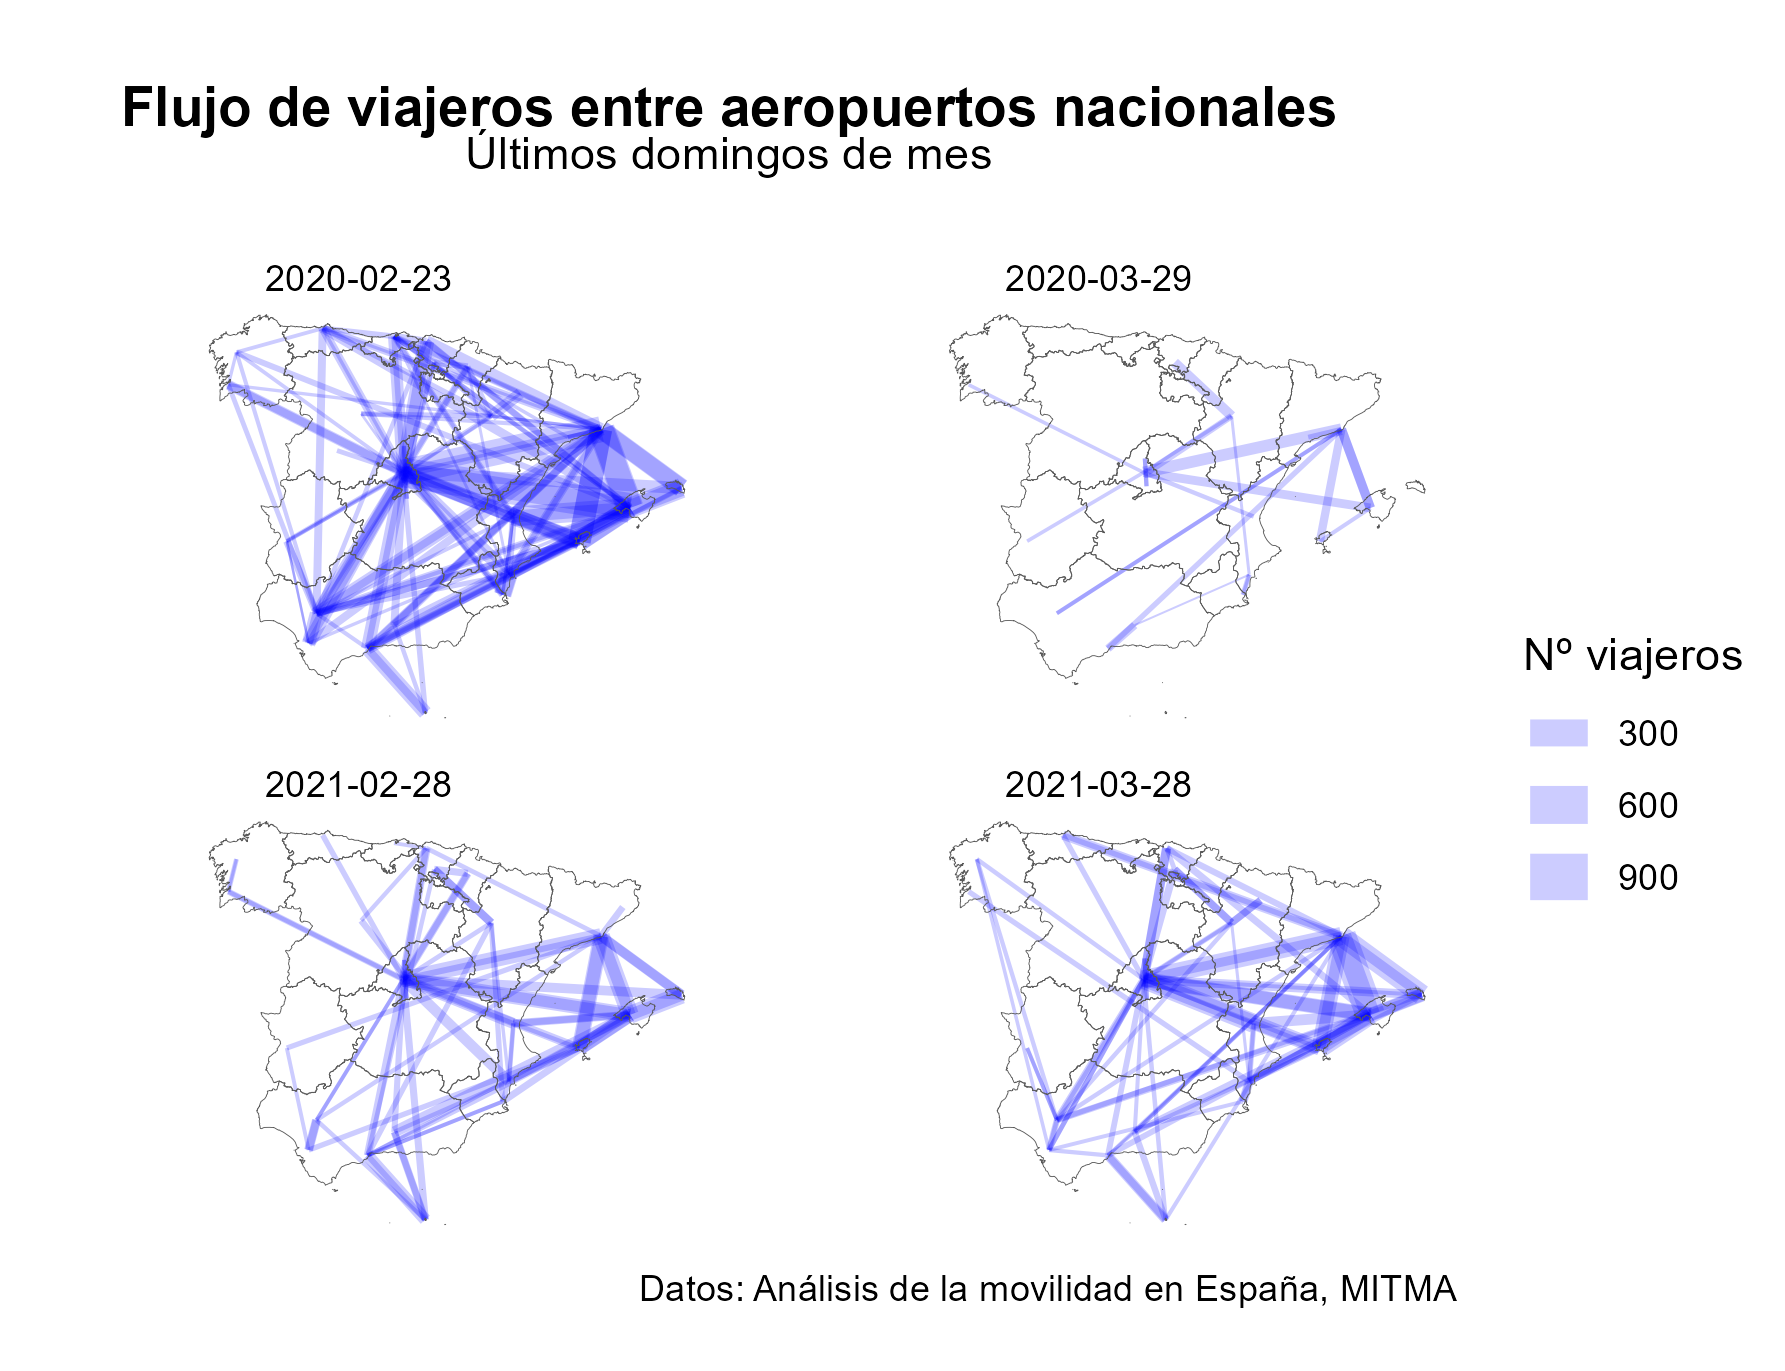
\includegraphics[width=0.6\linewidth]{img/movilidad_covid} 

}

\caption{Análisis de movilidad COVID}\label{fig:mov}
\end{figure}

\hypertarget{datos-geogruxe1ficos}{%
\chapter{Datos geográficos}\label{datos-geogruxe1ficos}}

\hypertarget{contexto-general}{%
\section{Contexto general}\label{contexto-general}}

La palabra geográfico puede dividirse en \textbf{geo} (tierra) + \textbf{gráfico}
(dibujo/mapa). Por tanto, los datos geográficos contienen información de
cualquier variable referenciada en un punto/área de la superficie terrestre y
pueden representarse en mapas. El desarrollo de los datos geográficos ha
producido grandes bases de datos espaciales y, a su vez, ha propiciado el
desarrollo de herramientas para su tratamiento como los ya mencionados Sistemas
de información geográficos y la Geocomputación.

\textbf{¿Qué hace un Sistemas de información geográfico?}

Un Sistema de información geográfica (SIG) es una herramienta que crea,
administra, analiza y mapea todo tipo de datos. GIS conecta datos a un mapa,
integrando datos de ubicación (\textbf{dónde} están las cosas) con todo tipo de
información descriptiva (\textbf{cómo} son las cosas allí).

Esto proporciona una base para el mapeo y el análisis que se utiliza en la
ciencia y en casi todas las industrias. GIS ayuda a los usuarios a comprender
patrones, relaciones y contexto geográfico. Los beneficios incluyen una mejor
comunicación y eficiencia, así como una mejor gestión y toma de decisiones.

La Fig. \ref{fig:gisflujo} muestra el flujo de trabajo de los SIG, que va desde
(i) la elaboración de mapas, (ii) la obtención de geodatos o datos espaciales,
(iii) el análisis de los datos geográficamente referenciados y (iv) la edición,
mapeo y presentación de los resultados.

\begin{figure}

{\centering 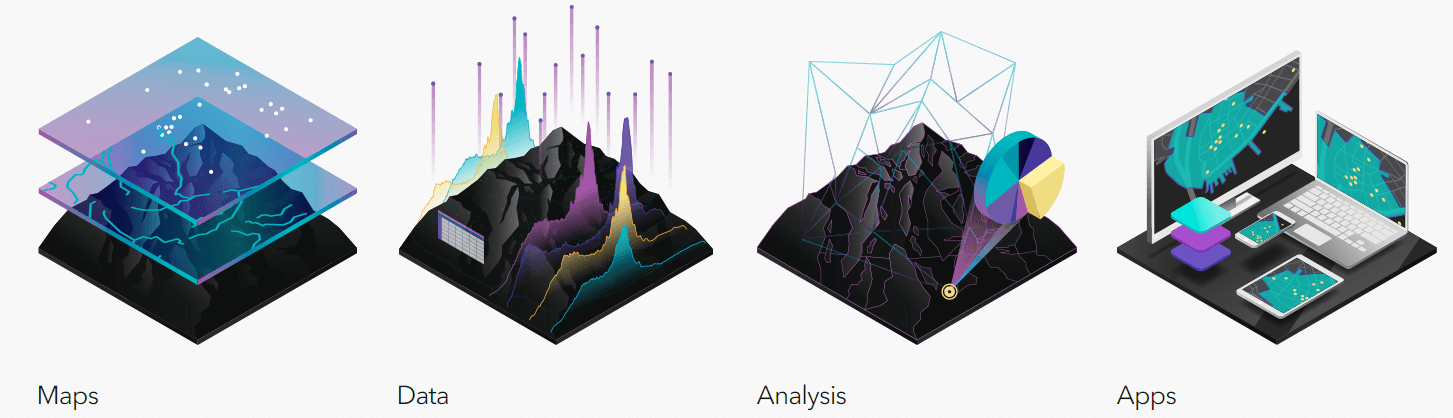
\includegraphics[width=0.7\linewidth]{img/GIS} 

}

\caption{Flujo de trabajo de los GIS. Fuente: https://www.esri.com/en-us/what-is-gis/overview}\label{fig:gisflujo}
\end{figure}

Pero es más, el desarrollo de la \textbf{Inteligencia Artificial} y la \textbf{Inteligencia
computacional} se han convertido en herramientas creativas y complementarias a
los convencionales GIS, dando origen a la \emph{Geocomputación}, que trata de
utilizar el \emph{poder de los ordenadores para hacer cosas con los datos
geográficos}.

\textbf{¿Y que es la Geocomputación?}

En primer lugar, señalar que, aunque la geocomputación es un término
relativamente nuevo se encuentra influenciado por otros términos clásicos. De
manera sencilla puede definirse como \emph{``el proceso de aplicar tecnologías de
computación a problemas geográficos''} \citep{rees1998}. \citet{Openshaw_Abrahart_2000}
aporta más elementos formales a esta definición destacando que \emph{``la
geocomputación trata sobre los diferentes tipos de geodatos, y sobre el
desarrollo de geo-herramientas relevantes en un contexto científico''}.

La geocomputación está muy relacionada con otros términos como los SIG, ya
definidos, y con diversos tipos de campos científicos, como las Geociencias, las
Ciencias atmosféricas y climáticas, la Geoinformática, la Topología, la Ecología
y las Ciencia de datos geográficos (GDS, Geographic Data Science).

Cada término comparte un énfasis en un enfoque \textbf{científico} (que implica
reproducible y falsable) influenciado por los GIS, aunque sus orígenes y
principales campos de aplicación difieren. La geocomputación es ámpliamente
utilizada en ámbitos como la sociología, el análisis político o el desarrollo de
aplicaciones para móviles. Por tanto, usamos geocomputación como un sinónimo
aproximado que encapsula a todas las ciencias que buscan usar datos geográficos
para trabajos científicos aplicados.

\textbf{¿Por que R para datos geográficos?}

R es una herramienta con capacidades avanzadas de análisis, modelado y
visualización. Por ejemplo, los nuevos entornos de desarrollo integrado (en
inglés, Integrated Development Environment, \textbf{IDE}), como RStudio, han hecho
que R sea más fácil de usar para muchos, facilitando la creación de mapas con un
panel dedicado a la visualización interactiva \citep{Lovelance_et_al_2019}. Además,
el uso del código R permite la enseñanza de la geocomputación con referencia a
ejemplos reproducibles en lugar de conceptos abstractos. Por ejemplo, de una
forma relativamente sencialla, se puede geoposicionar de manera interactiva la
localización de la Puerta del Sol en Madrid y, además, dejar la el código R para
hacerlo reproducible, ver Fig. \ref{fig:leaflet}.

\begin{Shaded}
\begin{Highlighting}[]
\FunctionTok{library}\NormalTok{(leaflet)}
\FunctionTok{leaflet}\NormalTok{(}\AttributeTok{width =} \StringTok{"100\%"}\NormalTok{, }\AttributeTok{height =} \StringTok{"500px"}\NormalTok{) }\SpecialCharTok{\%\textgreater{}\%}
  \FunctionTok{addTiles}\NormalTok{() }\SpecialCharTok{\%\textgreater{}\%}
  \FunctionTok{setView}\NormalTok{(}\SpecialCharTok{{-}}\FloatTok{3.703548}\NormalTok{, }\FloatTok{40.417147}\NormalTok{, }\AttributeTok{zoom =} \DecValTok{60}\NormalTok{)}
\end{Highlighting}
\end{Shaded}

\begin{figure}

{\centering 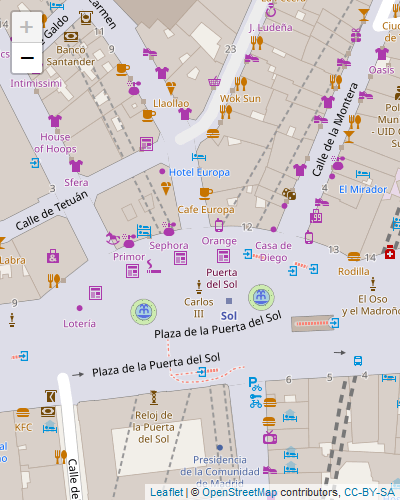
\includegraphics[width=0.6\linewidth]{_main_files/figure-latex/leaflet-1} 

}

\caption{Localización interactiva de la Puerta del Sol en Madrid}\label{fig:leaflet}
\end{figure}

Por otra parte R dispone de cientos de librerías especializadas para datos
espaciales. Una descripción detallada puede ver se en \href{https://cran.r-project.org/web/views/Spatial.html}{CRAN Task View: Analysis
of Spatial Data}

Para no abrumar al lector, a continuación se muestran, de manera esquemática,
las librerías más usadas para el tratamiento de datos espaciales y que se
emplearán a lo largo de la asignatura Estadística Espacial y Espacio-Temporal,
no sólo en el tema que nos ocupa:

\begin{itemize}
\item
  \texttt{sp} y \texttt{sf}: para el tratamiento de clases y métodos de los datos
  vectoriales.
\item
  \texttt{raster},\texttt{terra} y \texttt{stars} para datos raster.
\item
  \texttt{gstat} y \texttt{geoR}: para el análisis de datos geoestadísticos, ajuste y
  estimación de semivariogramas, interpolación, etc.
\item
  \texttt{spdep} para el análisis de datos con modelos de econometría espacial,
  creación de matrices de contiguidad/distancia \textbf{W}, estimación de modelos
  econométricos espaciales, etc
\item
  \texttt{spatstat} para el análisis de procesos de puntos espaciales, intensidad,
  etc.
\end{itemize}

\hypertarget{conceptos-clave}{%
\section{Conceptos clave}\label{conceptos-clave}}

Una vez visto el contexto actual de los datos georreferenciados y antes de
entrar en detalle en su análisis, debemos tener en cuenta una serie de conceptos
clave que se irán desarrollando a lo largo del tema.

Hemos dicho que Geográfico = Geo (tierra) + gráfico (mapa). Por tanto, si
tenemos varios datos geográficos, localizados en distintos puntos de la tierra,
es porque tenemos las \textbf{coordenadas} que los posicionan en esos puntos
concretos. Asociado a estas coordenadas debemos conocer el \textbf{Sistema de
referencia de espacial} o Coordinate reference system (CRS) en el que están
proyectadas dichas coordenadas.

Por otra parte, los formatos de estos datos pueden ser \textbf{vectores} o \textbf{raster}
como se explicará en la Sección \ref{formatos}.

Si damos un paso más e incorporamos el concepto de \textbf{distancia}, pues es lógico
pensar que en un fenómeno de interés, por ejemplo, la modelización de la
cantidad y dirección de lava en La Palma tras la erupción del volcán ``Cumbre
Vieja'', la distancia es un factor clave, pues aquellas zonas más cercanas al
volcán tendrán niveles más parecidos entre sí y con valores más altos que
aquellas que están más alejadas

En este caso el nivel de contaminación en el aire en La Palma no puede ser
modelado como si las observaciones fuesen independientes pues las más cercanas
entre sí serán más parecidas que las más lejanas, dando lugar al concepto de
\textbf{dependencia espacial}. Y depende del tipo de datos espaciales tendremos tres
grandes formas de abordar el tratamiento de los datos espaciales:
\textbf{geoestadística}, \textbf{procesos de punto} y \textbf{econometría espacial} (véase
sección \ref{CRS}).

\begin{figure}

{\centering 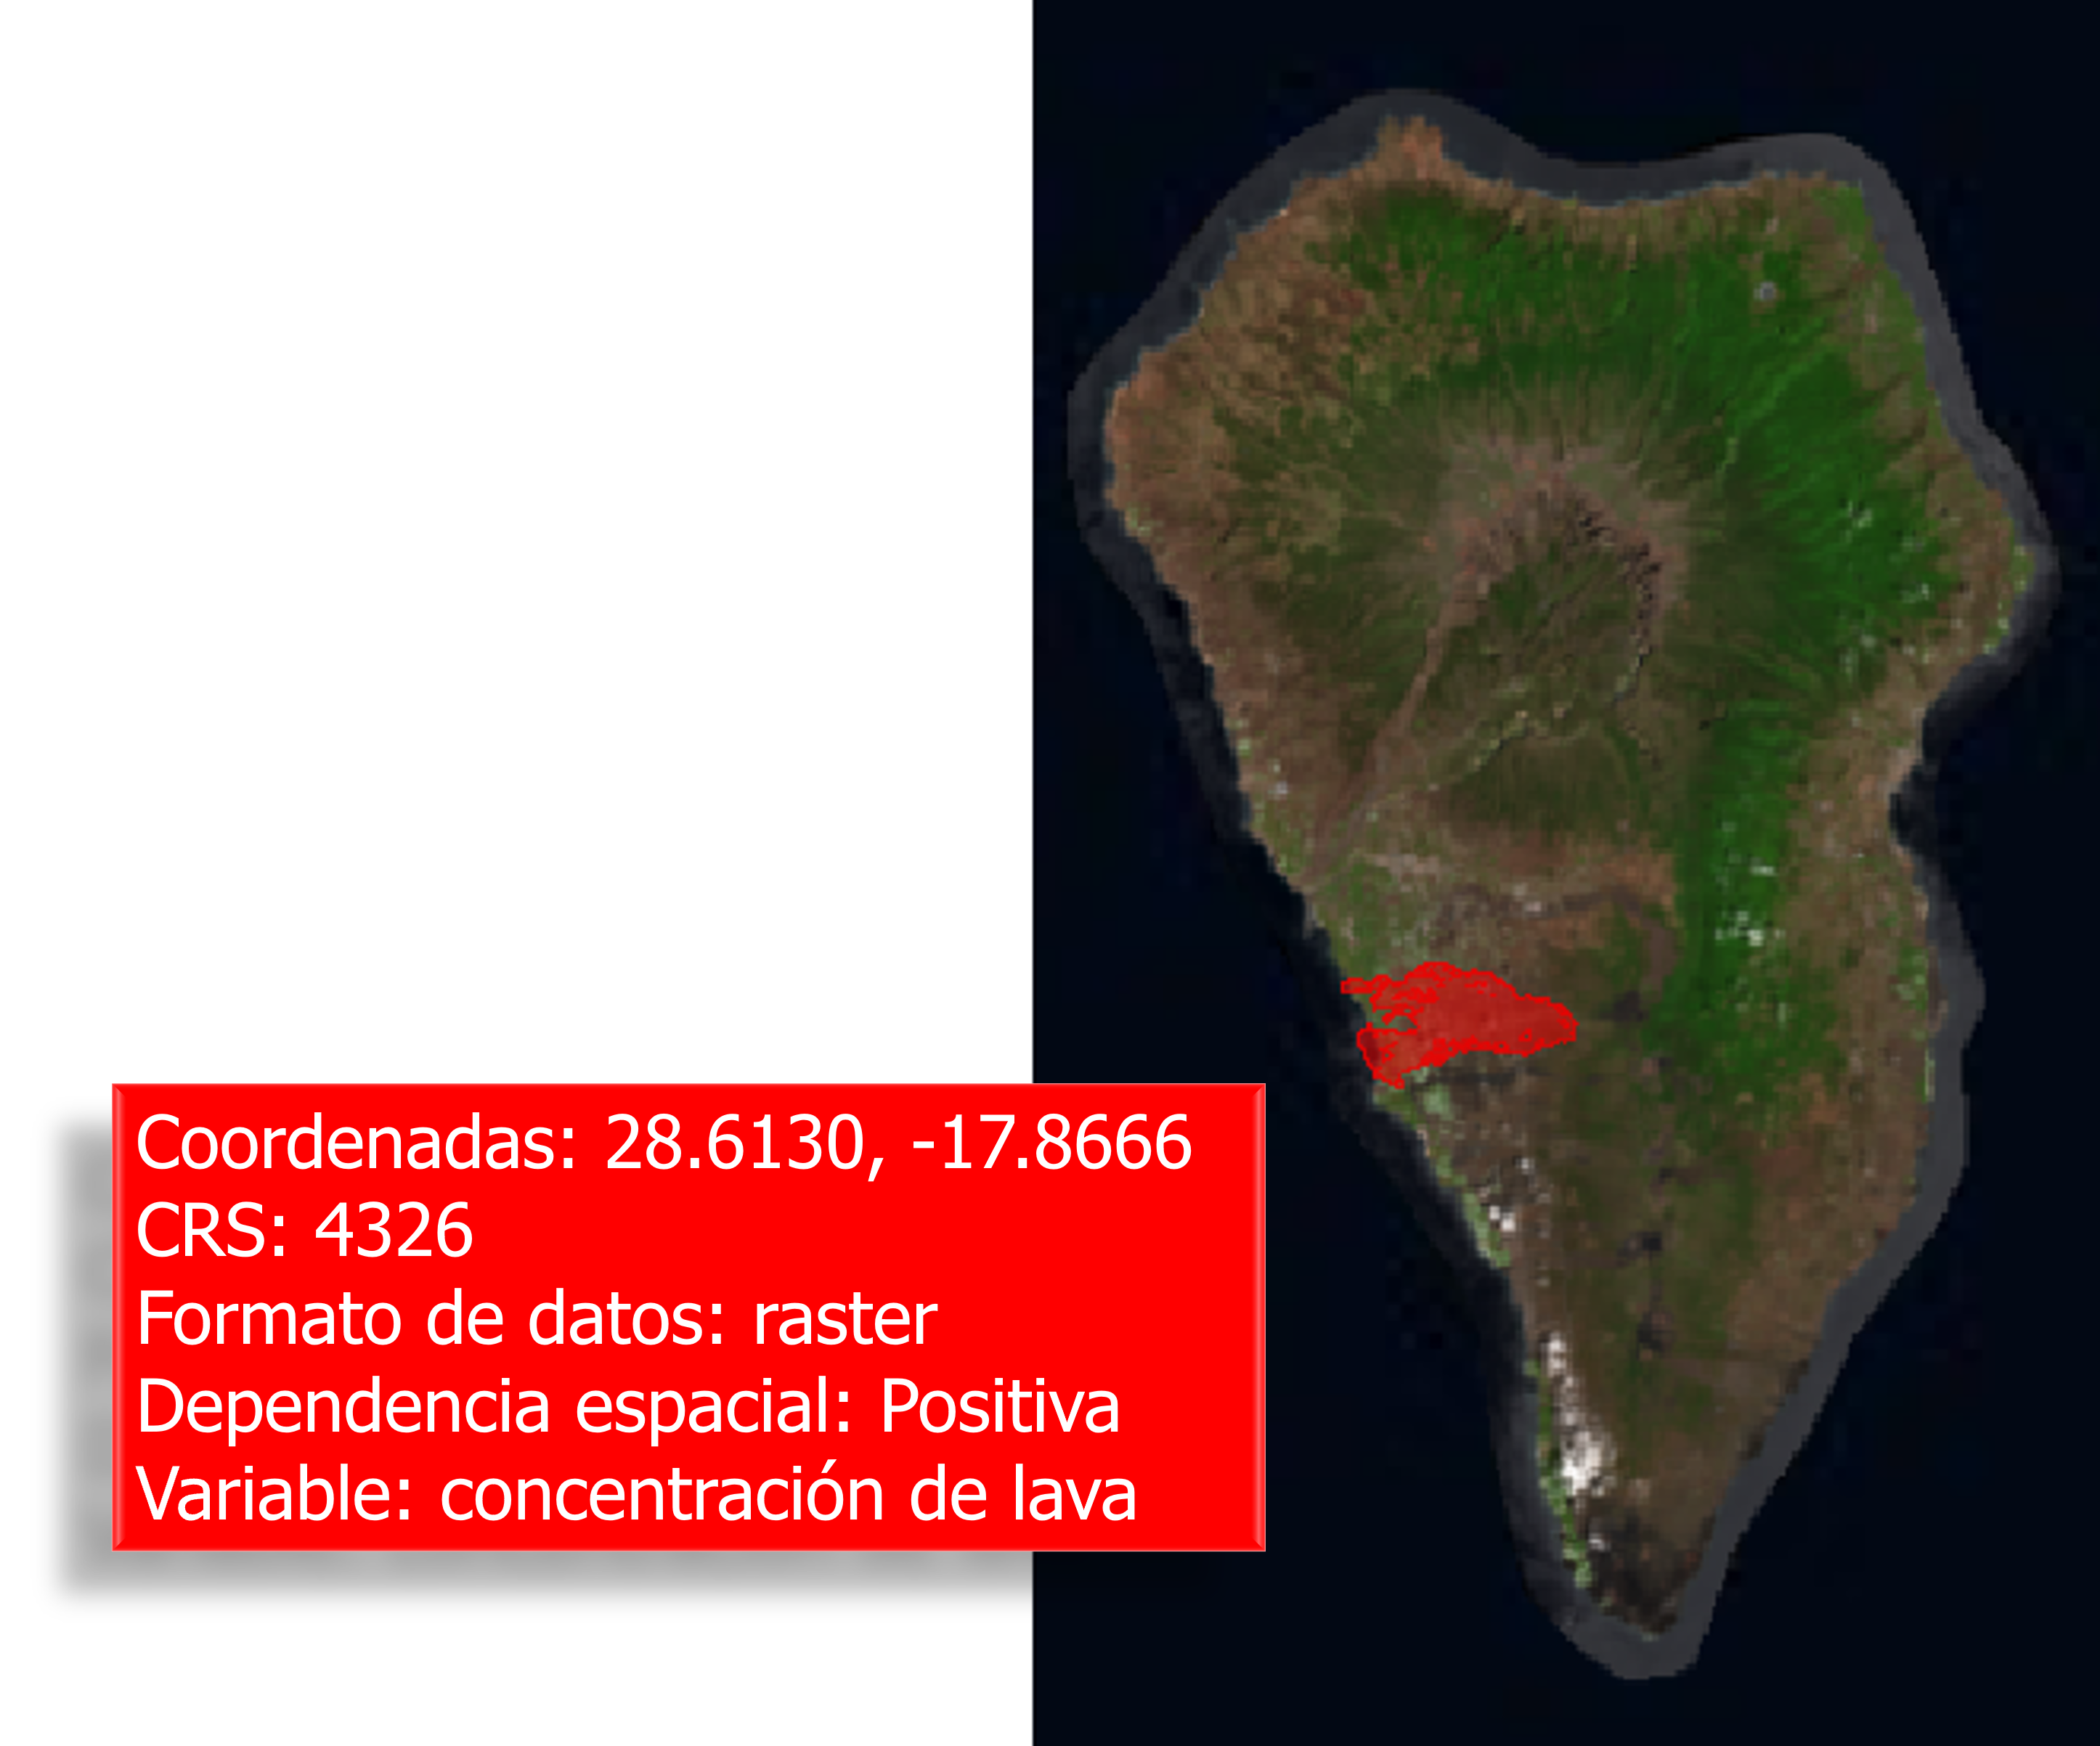
\includegraphics[width=0.6\linewidth]{img/Cumbrevieja} 

}

\caption{Información espacial de la concentración de lava en Cumbre Vieja}\label{fig:gis}
\end{figure}

\hypertarget{formatos}{%
\chapter{Formatos de datos espaciales}\label{formatos}}

\hypertarget{tipos-de-ficheros-completar}{%
\section{Tipos de ficheros (COMPLETAR)}\label{tipos-de-ficheros-completar}}

Poner el esquema de los Shapes.

\url{https://en.wikipedia.org/wiki/Shapefile}

Yo no sé, DIEGO, si en gisco R tienes la definición y lo ponemos de ahí.

Y pensar si tiene que venir aquí o dónde\ldots{} quizá al final de la sección
FORMATOS DE DATOS ESPACIALES

En el ámbito del análisis espacial en \textbf{R}, se pueden clasificar \textbf{el formato}
de datos espaciales en función del modelo de datos \citep{Lovelance_et_al_2019}. Se
pueden distinguir dos tipos de modelos de datos: vectores y raster.

\hypertarget{datos-de-vectores}{%
\section{Datos de vectores}\label{datos-de-vectores}}

Este modelo está basado en puntos georeferenciados. Los \textbf{puntos} pueden
representar localizaciones específicas, como la localización de edificios:

\begin{Shaded}
\begin{Highlighting}[]

\FunctionTok{library}\NormalTok{(ggplot2)}
\FunctionTok{library}\NormalTok{(sf)}


\CommentTok{\# Hospitales en Toledo segun Eurostat}
\NormalTok{hosp\_toledo }\OtherTok{\textless{}{-}} \FunctionTok{st\_read}\NormalTok{(}\StringTok{"data/hosp\_toledo.geojson"}\NormalTok{, }\AttributeTok{quiet =} \ConstantTok{TRUE}\NormalTok{)}

\CommentTok{\# Plot}
\FunctionTok{ggplot}\NormalTok{() }\SpecialCharTok{+}
  \FunctionTok{geom\_sf}\NormalTok{(}
    \AttributeTok{data =}\NormalTok{ hosp\_toledo, }\FunctionTok{aes}\NormalTok{(}\AttributeTok{fill =} \StringTok{"Centros Sanitarios"}\NormalTok{),}
    \AttributeTok{color =} \StringTok{"blue"}
\NormalTok{  ) }\SpecialCharTok{+}
  \FunctionTok{labs}\NormalTok{(}
    \AttributeTok{caption =} \StringTok{"Datos: Eurostat"}\NormalTok{,}
    \AttributeTok{title =} \StringTok{"Hospitales y Centros de Salud en Toledo"}\NormalTok{,}
    \AttributeTok{fill =} \StringTok{""}
\NormalTok{  ) }\SpecialCharTok{+}
  \FunctionTok{theme\_minimal}\NormalTok{() }\SpecialCharTok{+}
  \FunctionTok{theme}\NormalTok{(}\AttributeTok{legend.position =} \StringTok{"bottom"}\NormalTok{)}
\end{Highlighting}
\end{Shaded}

\begin{figure}

{\centering 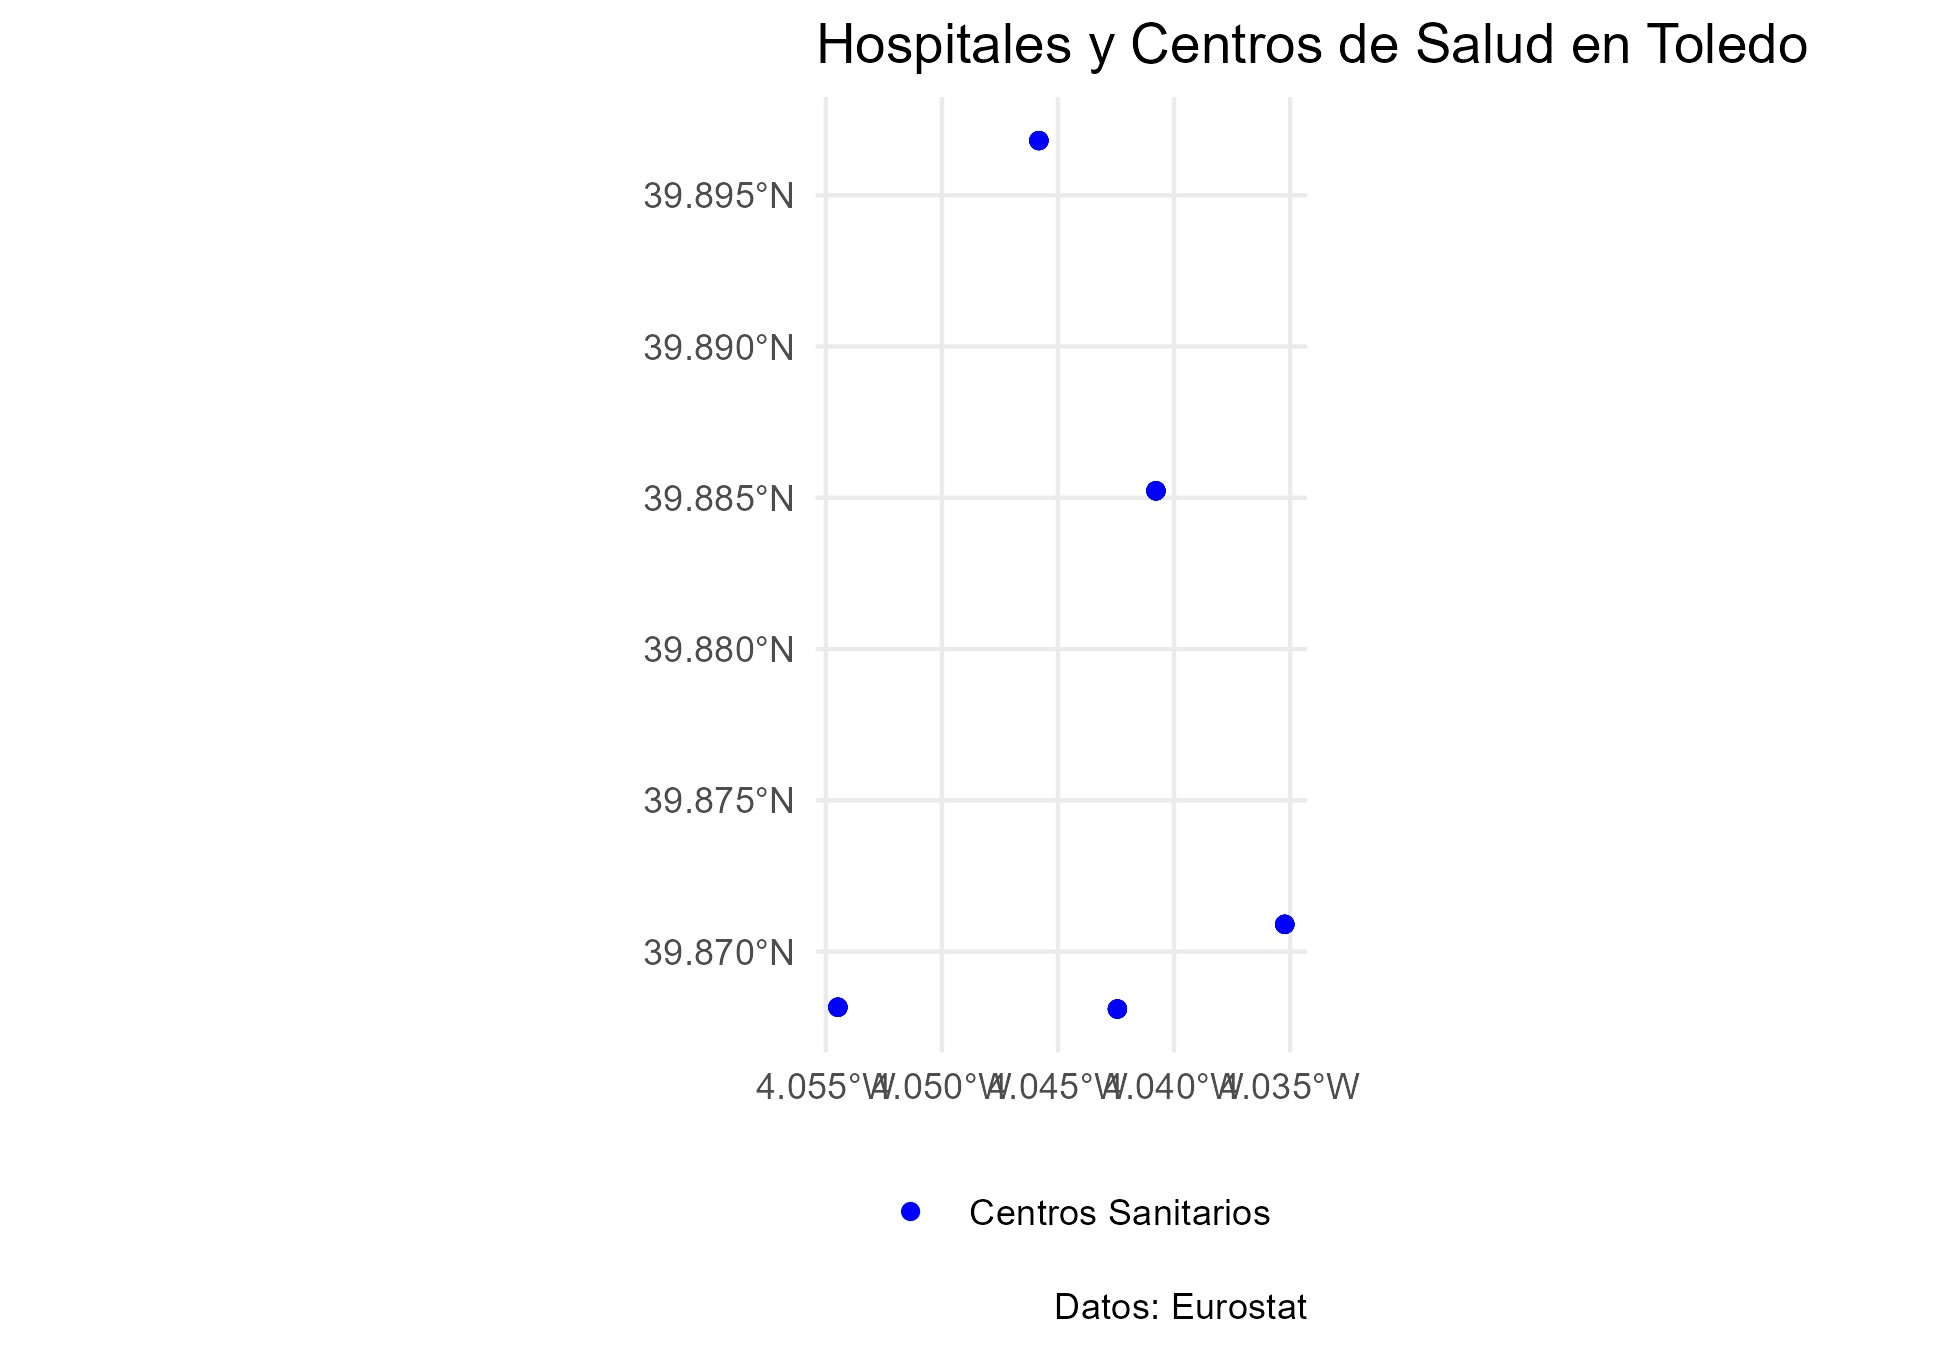
\includegraphics[width=0.6\linewidth]{_main_files/figure-latex/puntos-1} 

}

\caption{Datos vector: Puntos}\label{fig:puntos}
\end{figure}

Estos puntos también pueden estar conectados entre sí, de manera que formen
geometrías más complejas, como \textbf{líneas} y \textbf{polígonos}:

\begin{Shaded}
\begin{Highlighting}[]

\NormalTok{tajo }\OtherTok{\textless{}{-}} \FunctionTok{st\_read}\NormalTok{(}\StringTok{"data/tajo\_toledo.shp"}\NormalTok{, }\AttributeTok{quiet =} \ConstantTok{TRUE}\NormalTok{)}
\NormalTok{toledo }\OtherTok{\textless{}{-}} \FunctionTok{st\_read}\NormalTok{(}\StringTok{"data/toledo\_ciudad.gpkg"}\NormalTok{, }\AttributeTok{quiet =} \ConstantTok{TRUE}\NormalTok{)}


\FunctionTok{ggplot}\NormalTok{(toledo) }\SpecialCharTok{+}
  \FunctionTok{geom\_sf}\NormalTok{(}\AttributeTok{fill =} \StringTok{"cornsilk2"}\NormalTok{) }\SpecialCharTok{+}
  \FunctionTok{geom\_sf}\NormalTok{(}\AttributeTok{data =}\NormalTok{ tajo, }\AttributeTok{col =} \StringTok{"lightblue2"}\NormalTok{, }\AttributeTok{lwd =} \DecValTok{2}\NormalTok{, }\AttributeTok{alpha =} \FloatTok{0.7}\NormalTok{) }\SpecialCharTok{+}
  \FunctionTok{geom\_sf}\NormalTok{(}\AttributeTok{data =}\NormalTok{ hosp\_toledo, }\AttributeTok{col =} \StringTok{"blue"}\NormalTok{) }\SpecialCharTok{+}
  \FunctionTok{coord\_sf}\NormalTok{(}
    \AttributeTok{xlim =} \FunctionTok{c}\NormalTok{(}\SpecialCharTok{{-}}\FloatTok{4.2}\NormalTok{, }\SpecialCharTok{{-}}\FloatTok{3.8}\NormalTok{),}
    \AttributeTok{ylim =} \FunctionTok{c}\NormalTok{(}\FloatTok{39.8}\NormalTok{, }\FloatTok{39.95}\NormalTok{)}
\NormalTok{  ) }\SpecialCharTok{+}
  \FunctionTok{theme\_minimal}\NormalTok{()}
\end{Highlighting}
\end{Shaded}

\begin{figure}

{\centering 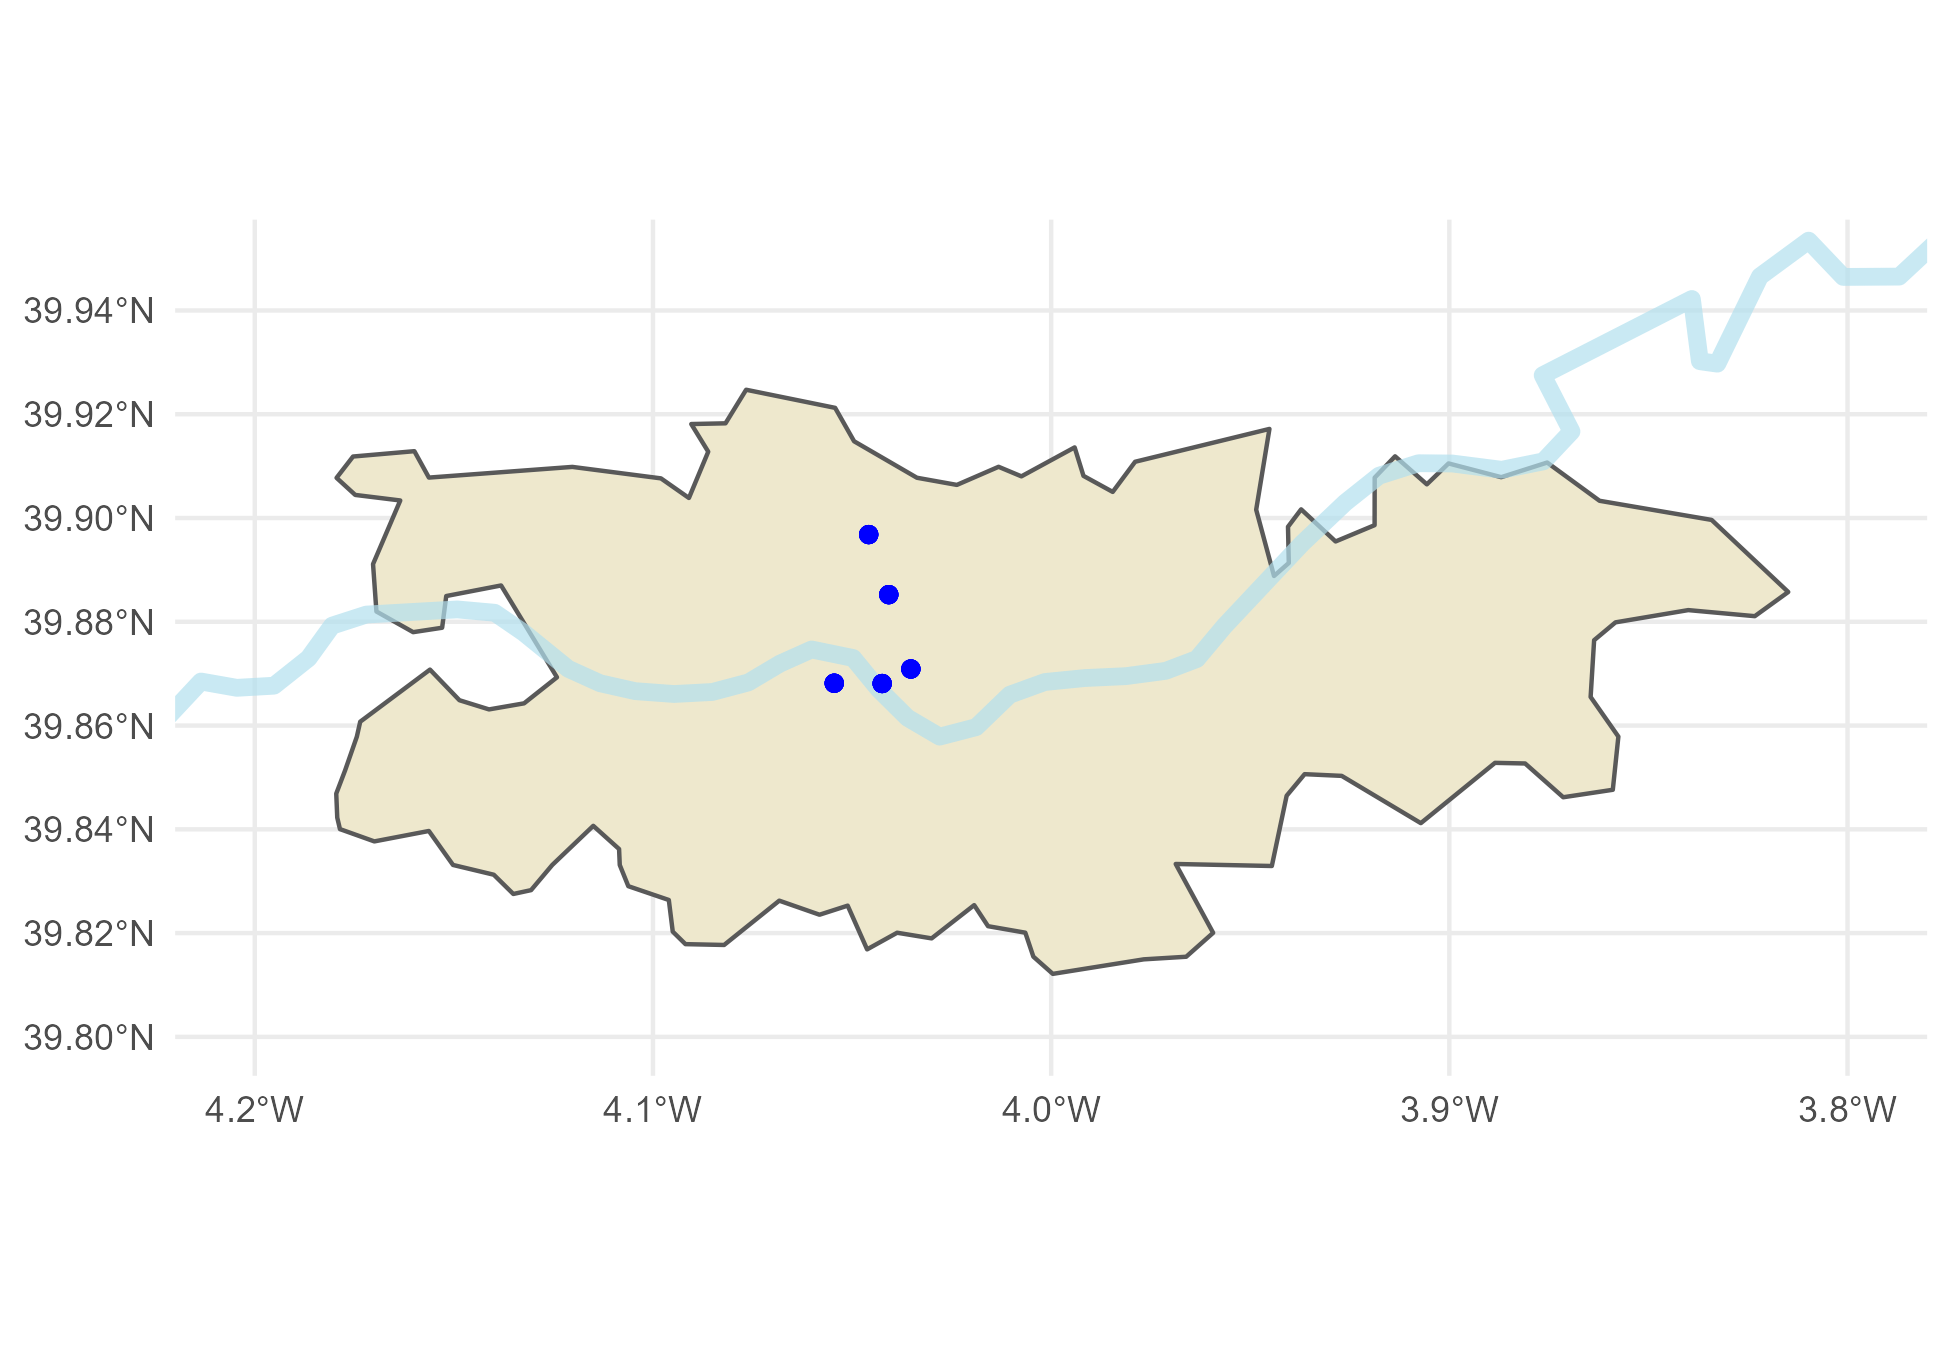
\includegraphics[width=0.6\linewidth]{_main_files/figure-latex/lineas-pol-1} 

}

\caption{Datos vector: Puntos, líneas y polígonos}\label{fig:lineas-pol}
\end{figure}

En la Fig. \ref{fig:lineas-pol}, el río Tajo está representado como una línea
(sucesión de puntos unidos entre sí) y la ciudad de Toledo como un polígono
(línea de puntos cerrada formando un continuo). A modo ilustrativo, la Fig.
\ref{fig:lineas-pol-desc} representa la descomposición en puntos de todos los
datos espaciales representados en la Fig. \ref{fig:lineas-pol}.

\begin{figure}

{\centering 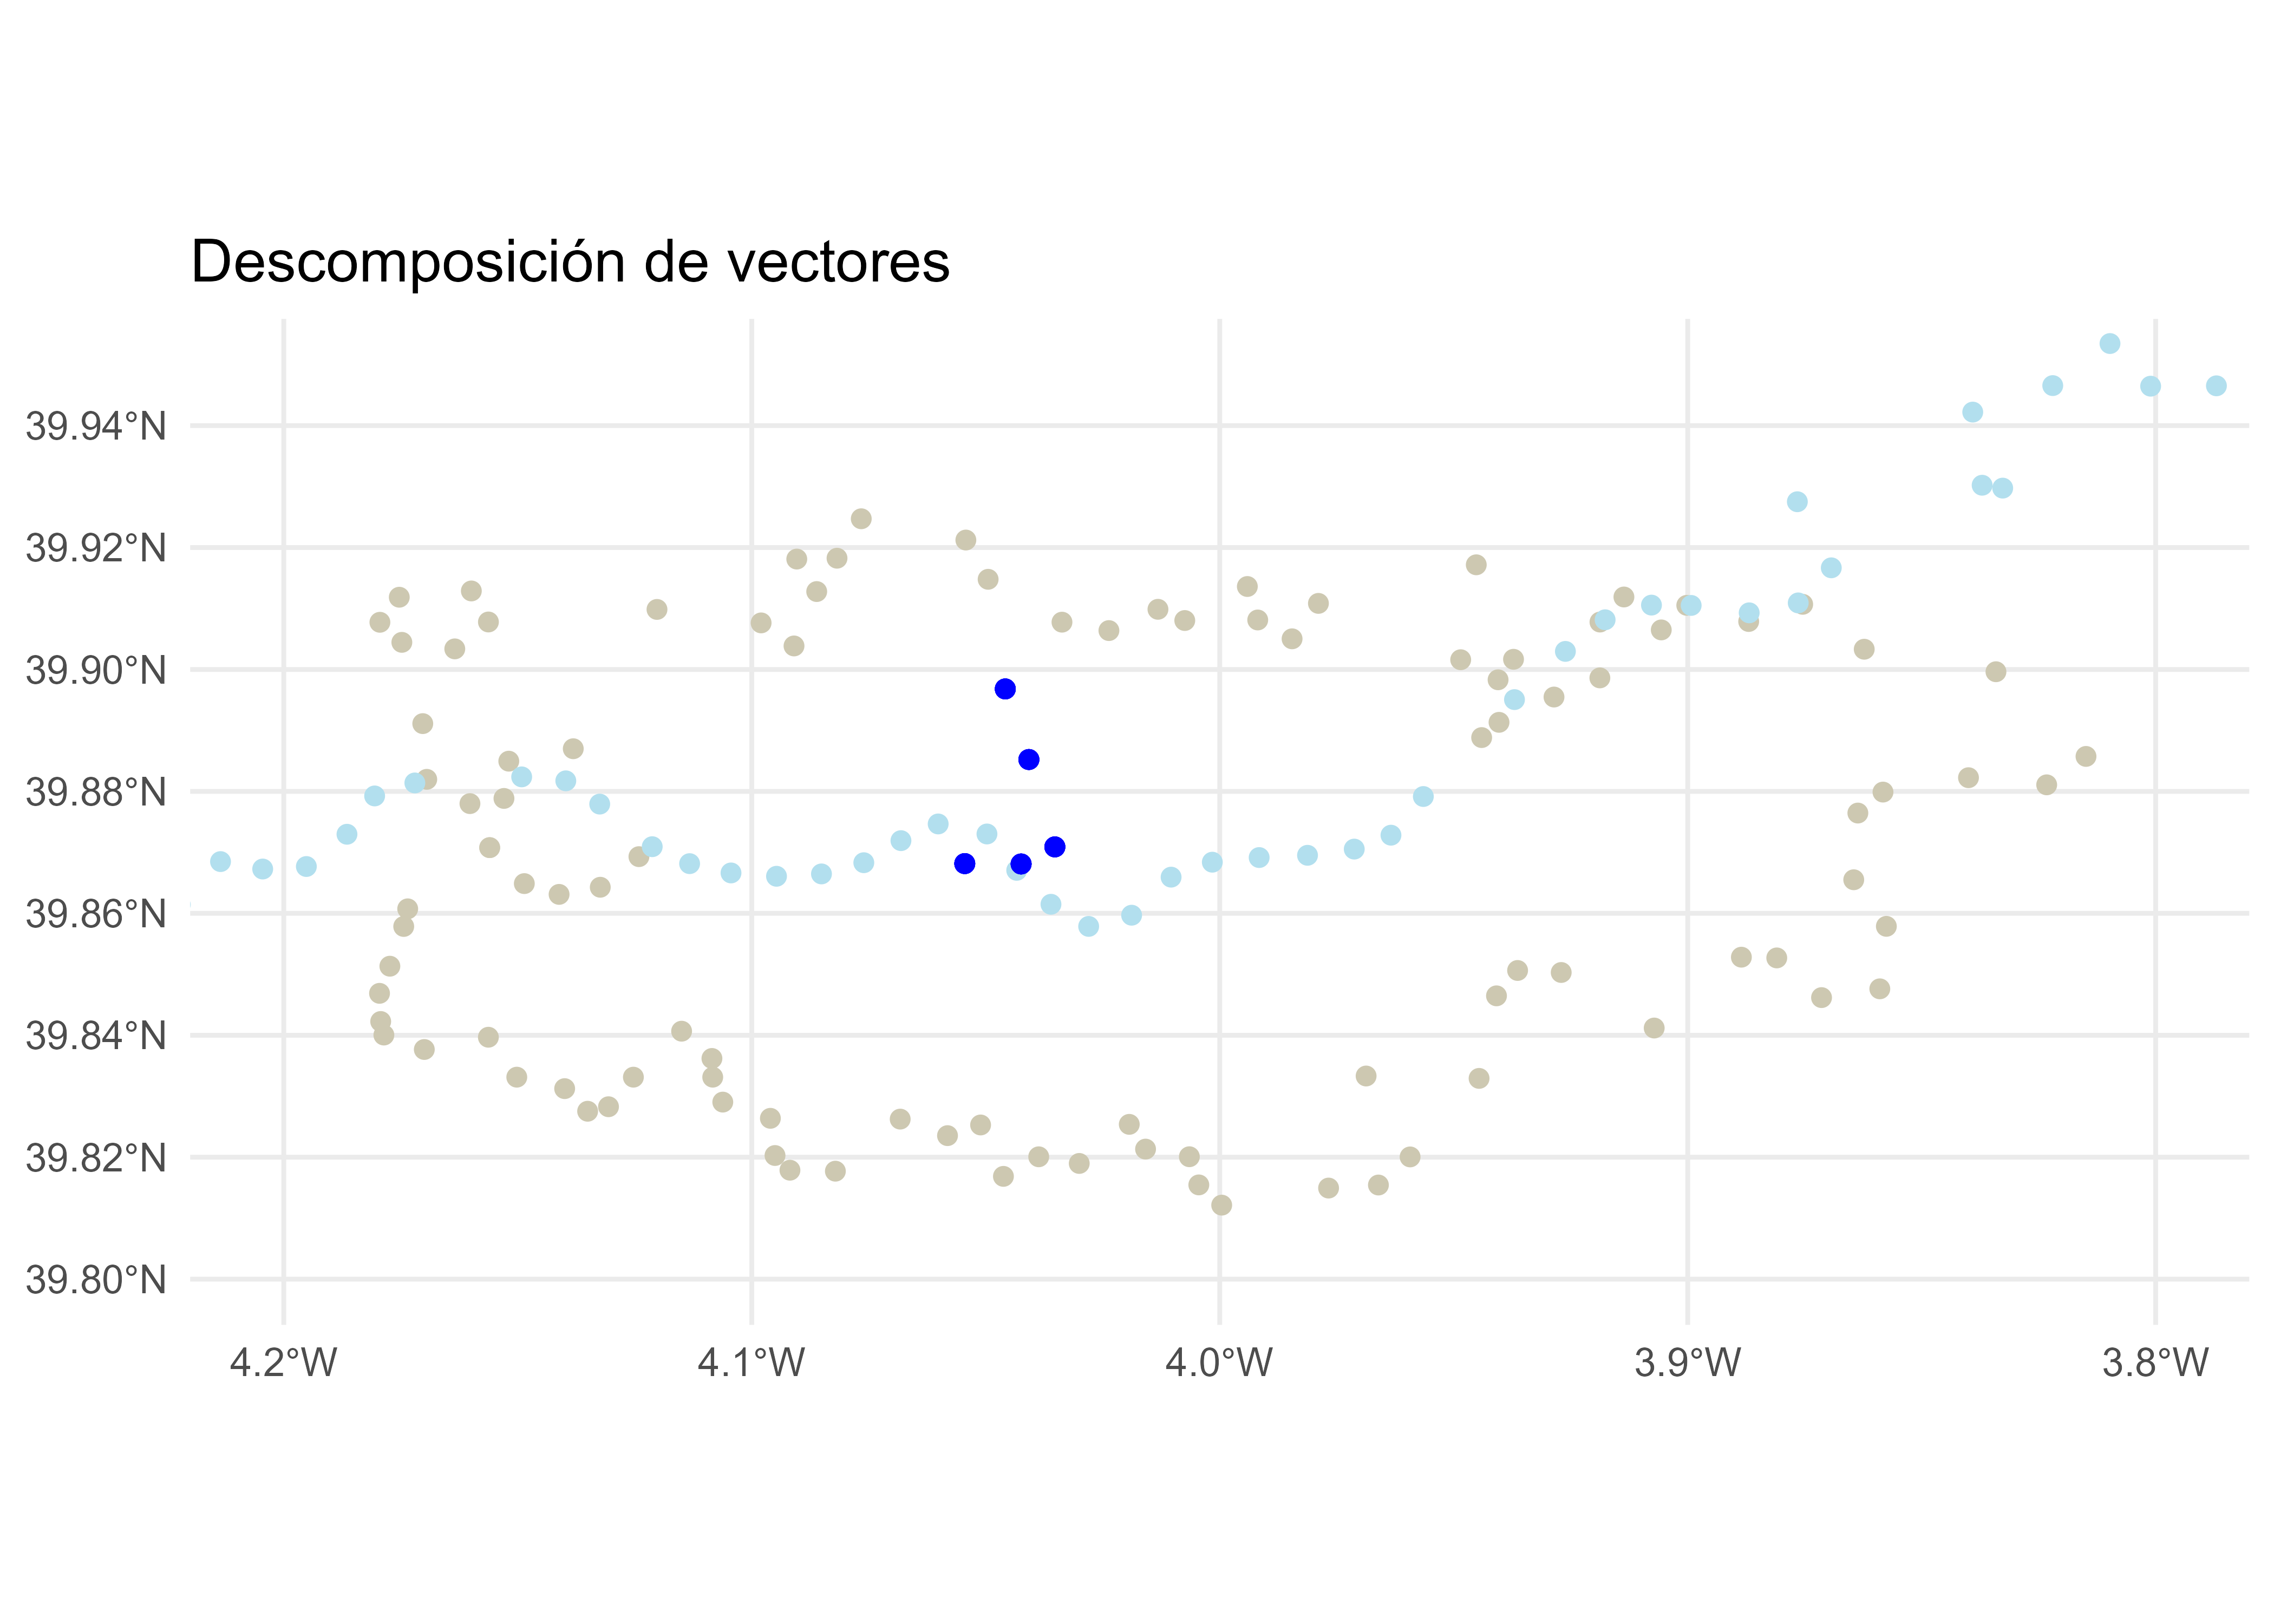
\includegraphics[width=0.6\linewidth]{_main_files/figure-latex/lineas-pol-desc-1} 

}

\caption{Datos vector: Descomposición en puntos}\label{fig:lineas-pol-desc}
\end{figure}

\hypertarget{datos-raster}{%
\section{Datos raster}\label{datos-raster}}

Los datos ráster son datos representandos en una rejilla rectangular de píxeles
(denomindada \textbf{matriz}) que se puede visualizar en diversos dispositivo de
representación. El caso más cotidiano de un ráster es una fotografía, donde la
imagen se representa como una serie de celdas, determinadas por la resolución de
la imagen (número total de píxeles, determinados como número de píxeles en cada
fila por número de píxeles en cada columna) y el color que presenta cada uno de
estos píxeles.

En el ámbito de los datos espaciales, la definición es muy similar. Un archivo
ráster está formado por una malla regular de píxeles georreferenciada, tal y
como muestra la Fig. \ref{fig:raster}:

\begin{Shaded}
\begin{Highlighting}[]

\FunctionTok{library}\NormalTok{(raster)}

\NormalTok{elev }\OtherTok{\textless{}{-}} \FunctionTok{raster}\NormalTok{(}\StringTok{"data/Toledo\_DEM.tiff"}\NormalTok{)}
\FunctionTok{plot}\NormalTok{(elev, }\AttributeTok{main =} \StringTok{"Elevación de la provincia de Toledo"}\NormalTok{)}

\CommentTok{\# Mostramos el grid}
\NormalTok{pols }\OtherTok{\textless{}{-}} \FunctionTok{rasterToPolygons}\NormalTok{(elev)}
\FunctionTok{plot}\NormalTok{(pols, }\AttributeTok{add =} \ConstantTok{TRUE}\NormalTok{, }\AttributeTok{border =} \StringTok{"grey90"}\NormalTok{)}

\CommentTok{\# Añadimos la provincia}
\NormalTok{Tol\_prov }\OtherTok{\textless{}{-}} \FunctionTok{st\_read}\NormalTok{(}\StringTok{"data/Toledo\_prov.gpkg"}\NormalTok{, }\AttributeTok{quiet =} \ConstantTok{TRUE}\NormalTok{)}

\CommentTok{\# Si queremos solamente la forma en sf, usamos st\_geometry}
\FunctionTok{plot}\NormalTok{(}\FunctionTok{st\_geometry}\NormalTok{(Tol\_prov), }\AttributeTok{add =} \ConstantTok{TRUE}\NormalTok{)}
\end{Highlighting}
\end{Shaded}

\begin{figure}

{\centering 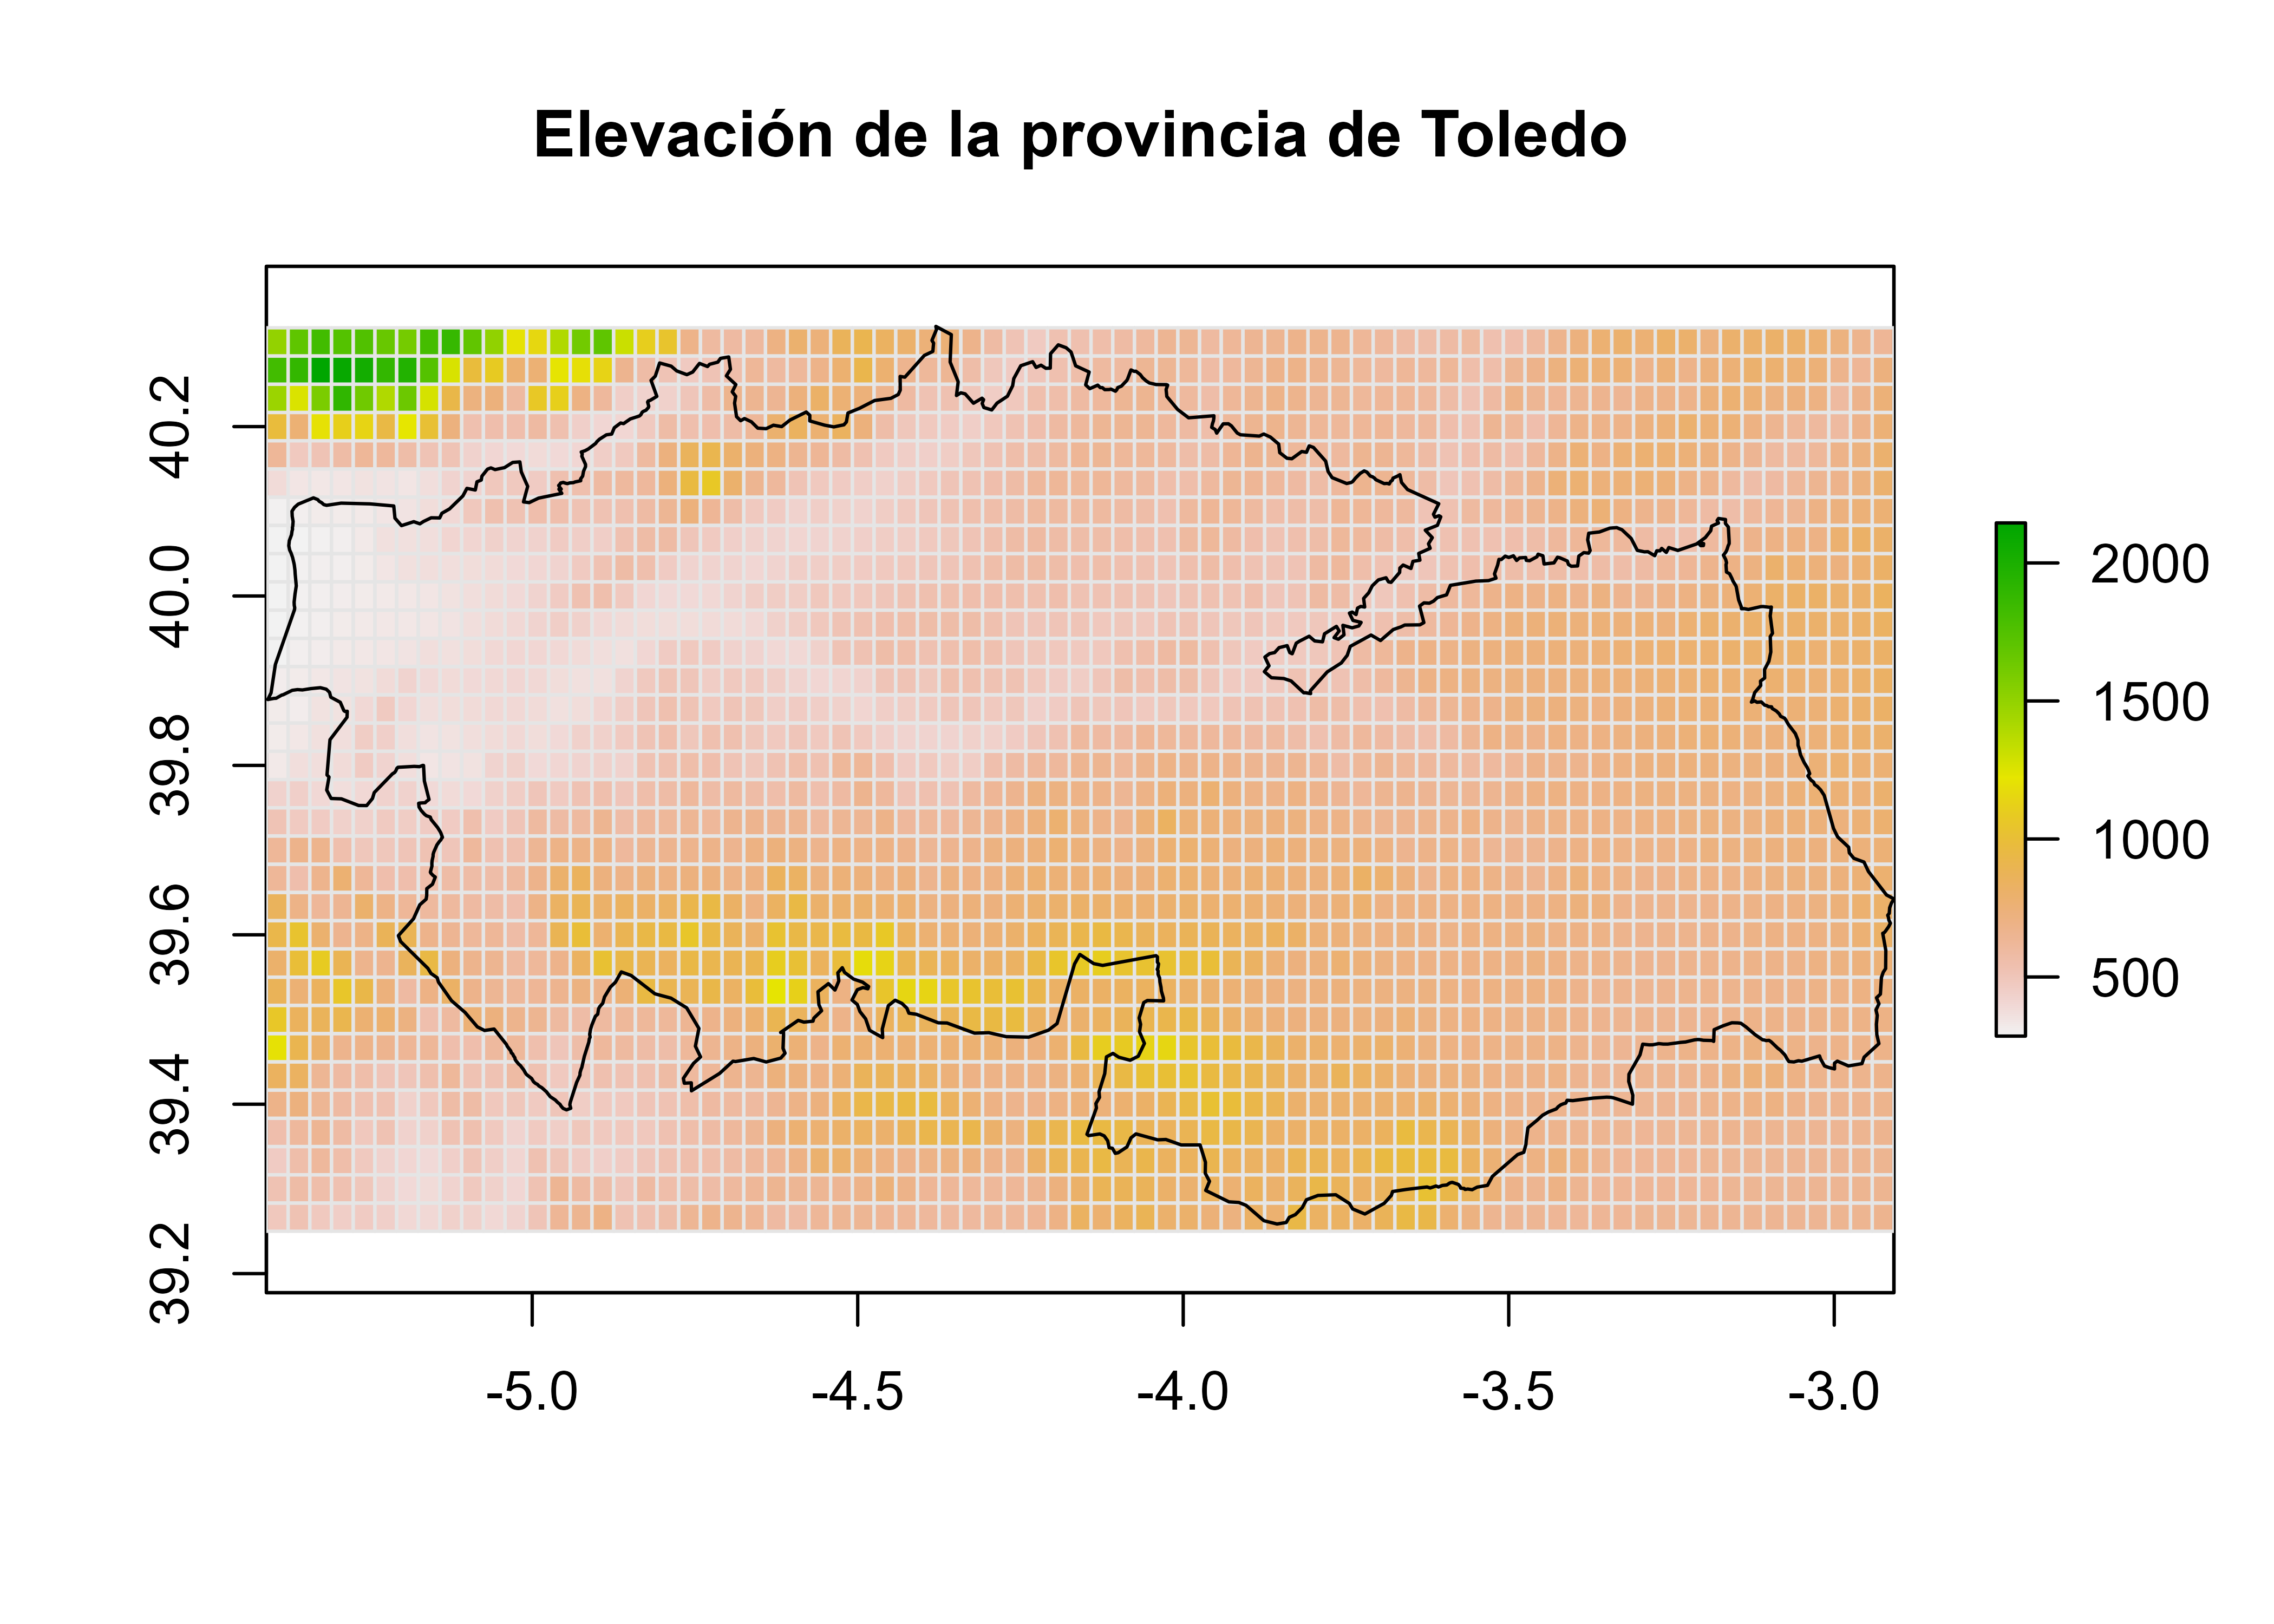
\includegraphics[width=0.6\linewidth]{_main_files/figure-latex/raster-1} 

}

\caption{Datos ráster}\label{fig:raster}
\end{figure}

En la Fig. \ref{fig:raster}, el objeto ráster \texttt{elev} tiene únicamente una capa
(denominada \texttt{ESP\_alt}). Eso implica que cada píxel tiene asociado un único
valor, en este caso, en este caso la altitud media del terreno observada:

\begin{table}

\caption{\label{tab:detalle-pixel}Datos de un ráster (detalle)}
\centering
\begin{tabular}[t]{r|r|r}
\hline
x & y & Toledo\_DEM\\
\hline
-5.391667 & 40.3 & 1498.312\\
\hline
-5.358333 & 40.3 & 1701.125\\
\hline
-5.325000 & 40.3 & 1825.312\\
\hline
-5.291667 & 40.3 & 1739.062\\
\hline
-5.258333 & 40.3 & 1756.062\\
\hline
-5.225000 & 40.3 & 1659.688\\
\hline
-5.191667 & 40.3 & 1607.375\\
\hline
-5.158333 & 40.3 & 1809.562\\
\hline
-5.125000 & 40.3 & 1874.625\\
\hline
-5.091667 & 40.3 & 1691.312\\
\hline
-5.058333 & 40.3 & 1511.500\\
\hline
-5.025000 & 40.3 & 1207.000\\
\hline
-4.991667 & 40.3 & 1160.125\\
\hline
-4.958333 & 40.3 & 1396.125\\
\hline
-4.925000 & 40.3 & 1624.125\\
\hline
\end{tabular}
\end{table}

\begin{figure}

{\centering 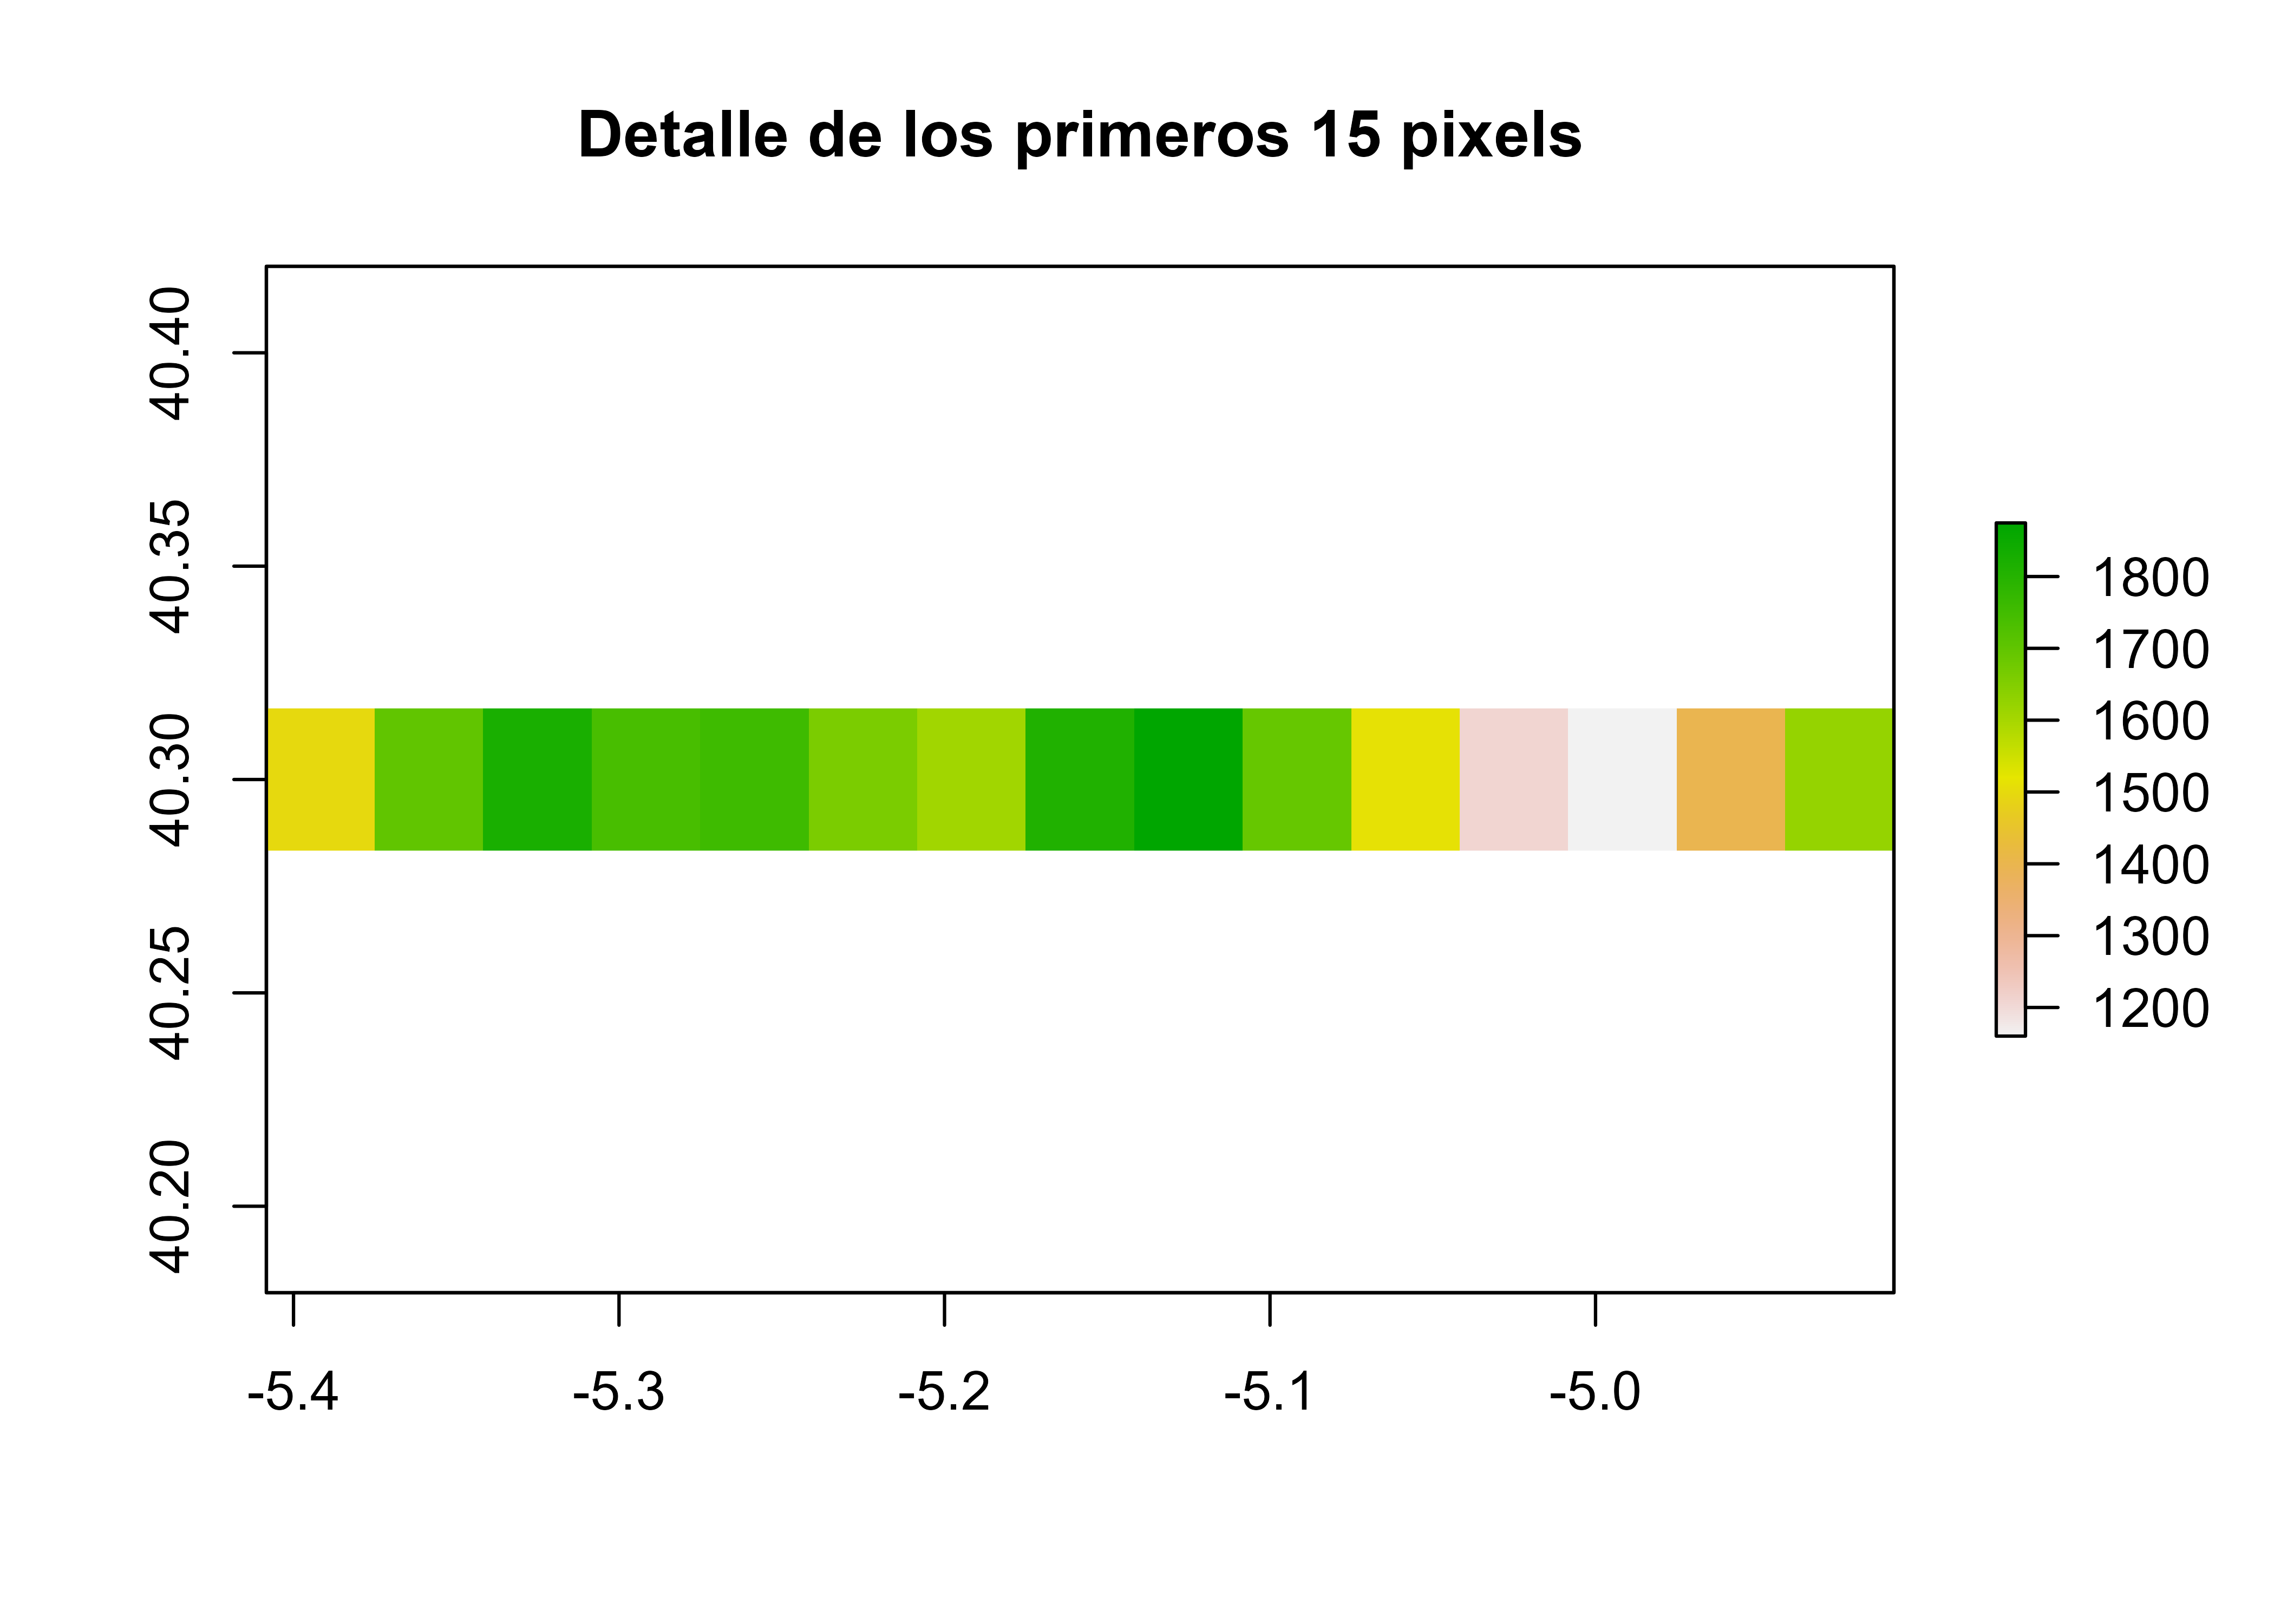
\includegraphics[width=0.6\linewidth]{_main_files/figure-latex/detalle-pixel-1} 

}

\caption{Datos ráster: Detalle}\label{fig:detalle-pixel}
\end{figure}

Los rásters pueden contener varias capas (o layers), de manera que cada píxel
puede tener asociados varios valores. Volviendo al ejemplo de la fotografía, en
un modelo simple de color RGB cada píxel lleva asociado 3 valores (rojo, verde o
azul), de manera que al combinar las tres capas se puede definir un color
distinto en cada píxel.

En la Fig. \ref{fig:raster-multilayer} vamos a usar una imagen de mapa
georreferenciada, como las proporcionadas por servicios de mapas online, para
analizar su composición.

\begin{figure}

{\centering 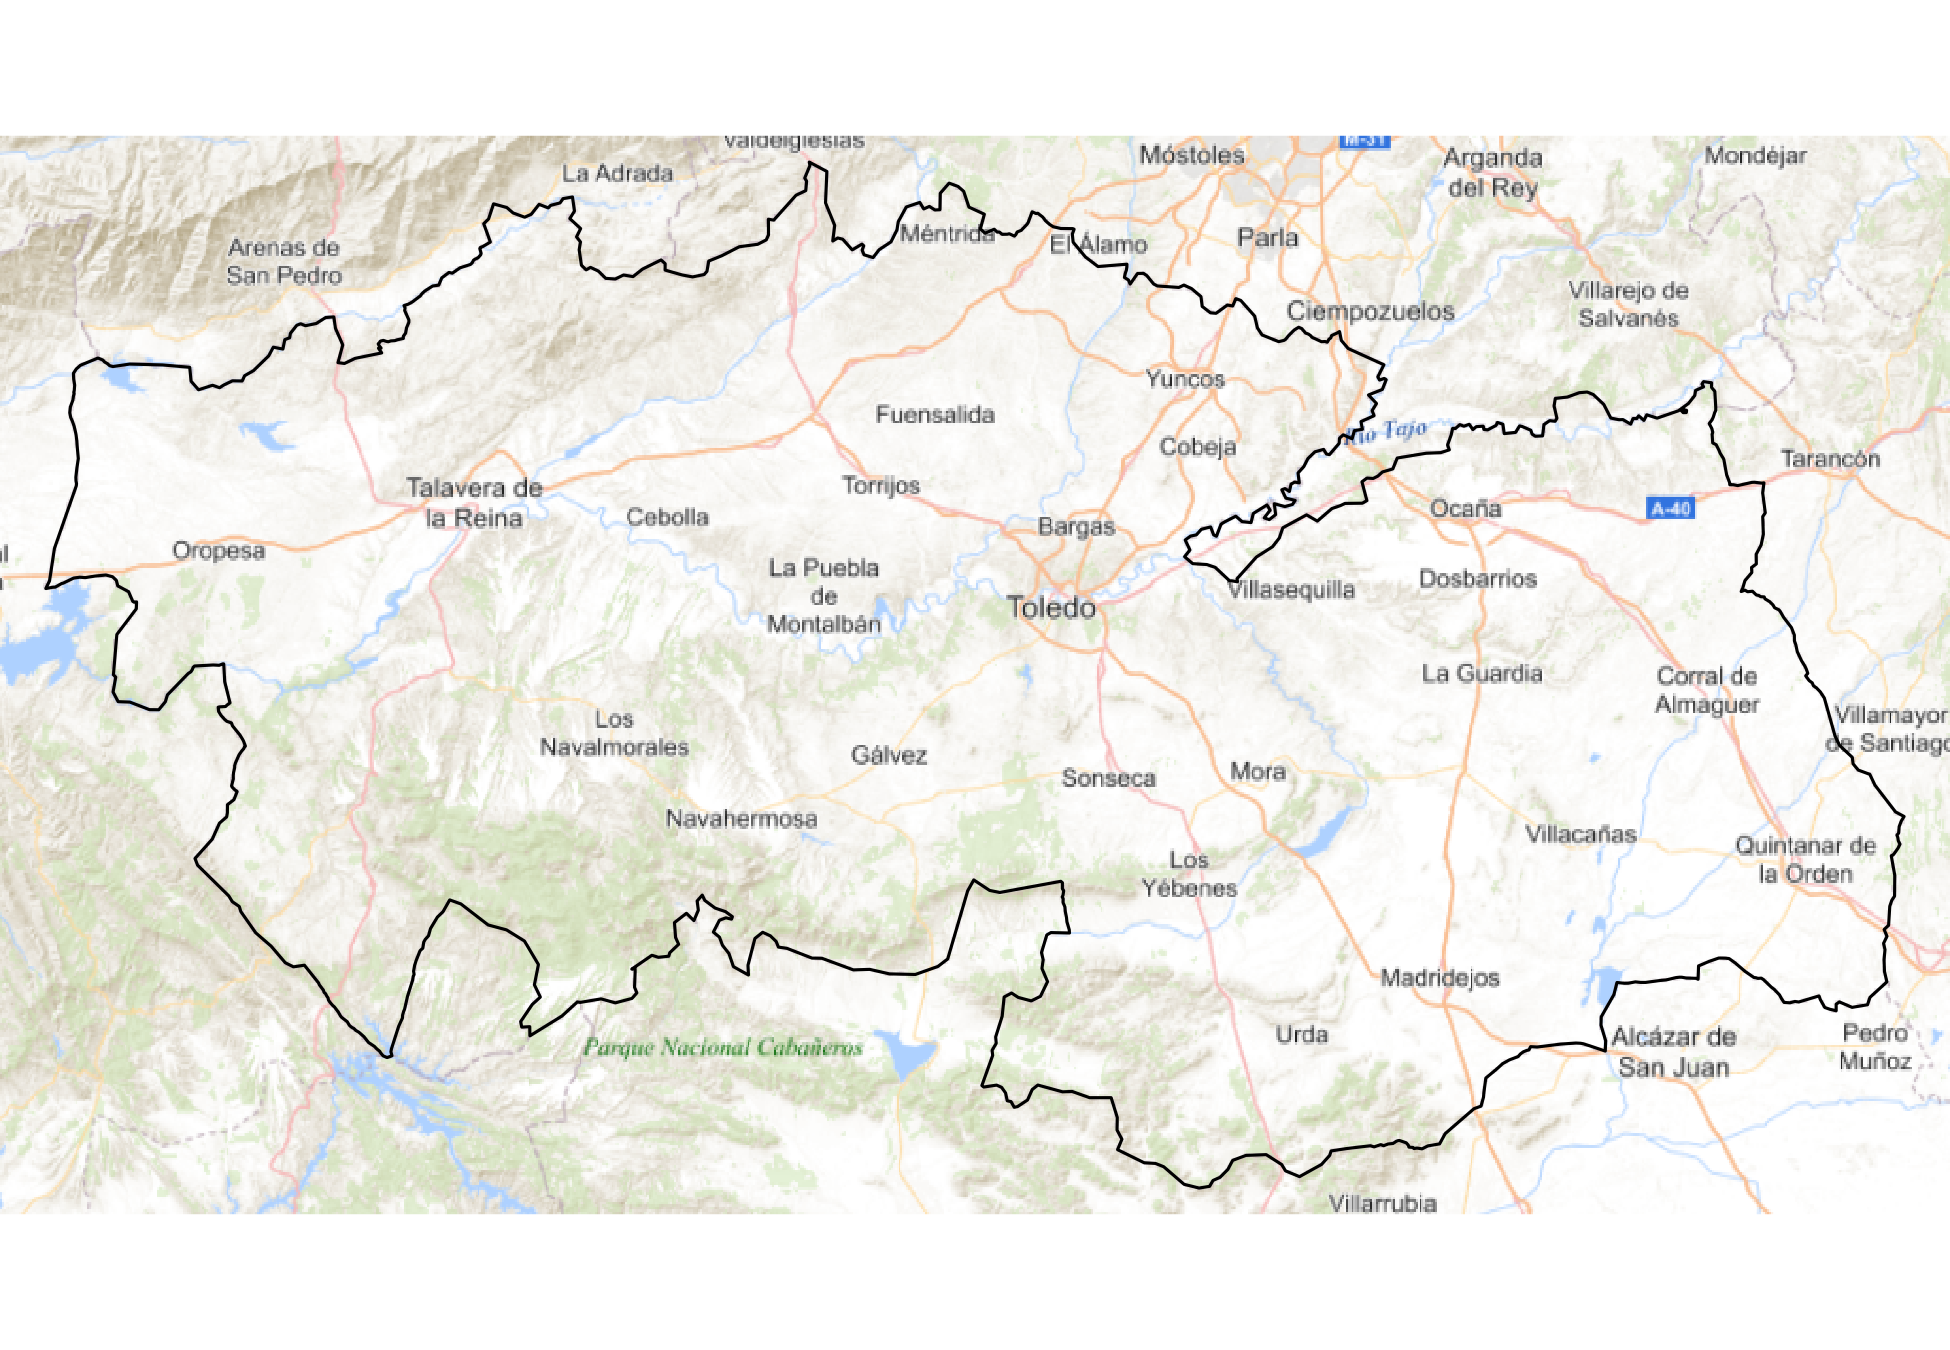
\includegraphics[width=0.6\linewidth]{_main_files/figure-latex/raster-multilayer-1} 

}

\caption{Datos ráster con varias bandas}\label{fig:raster-multilayer}
\end{figure}

El ráster se puede descomponer en las tres capas RGB mencionadas anteriormente:

\begin{table}

\caption{\label{tab:detalle-pixel-multicapa}Datos de un ráster multicapa (detalle)}
\centering
\begin{tabular}[t]{r|r|r|r|r}
\hline
x & y & lyr.1 & lyr.2 & lyr.3\\
\hline
-5.466412 & 40.34418 & 215.2128 & 208.1061 & 190.5410\\
\hline
-5.463875 & 40.34418 & 228.0369 & 223.1854 & 211.2115\\
\hline
-5.461338 & 40.34418 & 229.3495 & 224.3414 & 213.4325\\
\hline
-5.458800 & 40.34418 & 215.8592 & 208.8660 & 191.2922\\
\hline
-5.456263 & 40.34418 & 219.2696 & 212.8231 & 196.6812\\
\hline
-5.453725 & 40.34418 & 235.0954 & 231.4222 & 222.4115\\
\hline
-5.451188 & 40.34418 & 240.3514 & 237.9094 & 231.4736\\
\hline
-5.448651 & 40.34418 & 237.2358 & 233.7561 & 226.2005\\
\hline
-5.446113 & 40.34418 & 229.9570 & 225.3262 & 214.6201\\
\hline
-5.443576 & 40.34418 & 226.7812 & 221.6796 & 209.2929\\
\hline
-5.441038 & 40.34418 & 222.3593 & 216.5022 & 202.0188\\
\hline
-5.438501 & 40.34418 & 220.9312 & 214.9060 & 200.0306\\
\hline
-5.435964 & 40.34418 & 224.7755 & 219.2661 & 206.2156\\
\hline
-5.433426 & 40.34418 & 222.0479 & 216.0124 & 201.6103\\
\hline
-5.430889 & 40.34418 & 225.0516 & 219.8074 & 207.0263\\
\hline
\end{tabular}
\end{table}

\begin{figure}

{\centering 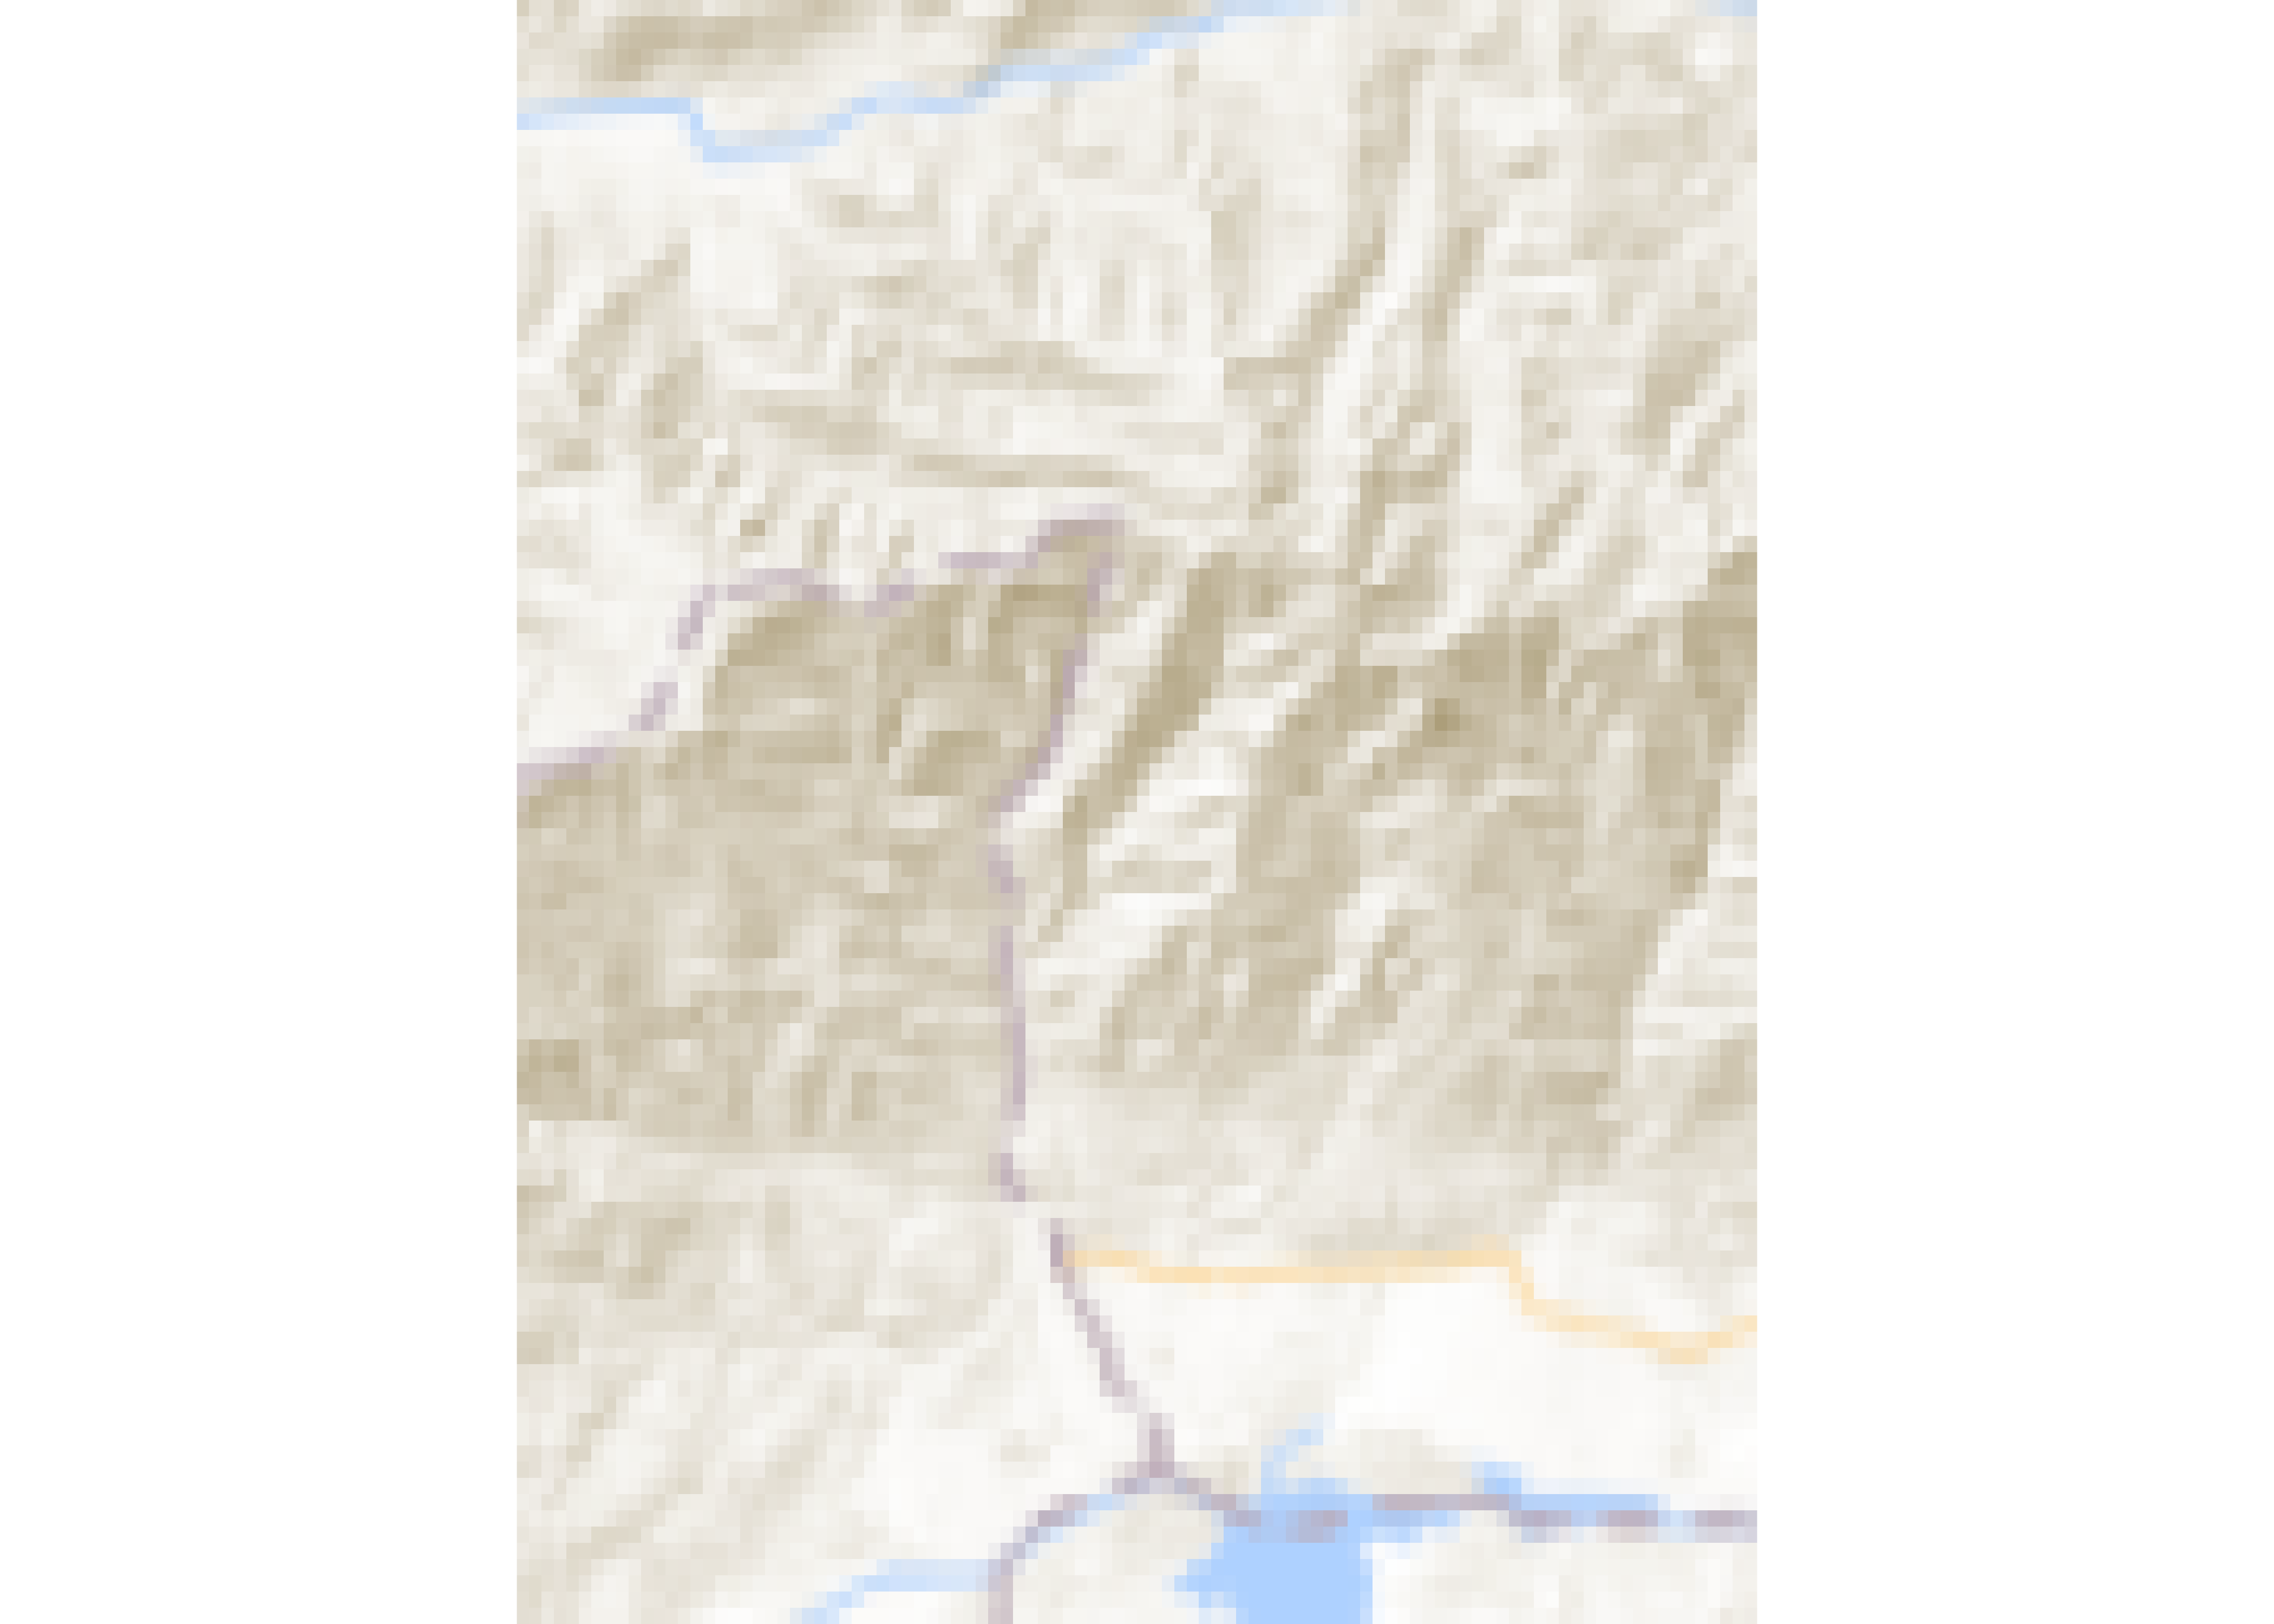
\includegraphics[width=0.6\linewidth]{_main_files/figure-latex/detalle-pixel-multicapa-1} 

}

\caption{Datos ráster multicapa: Descomposición}\label{fig:detalle-pixel-multicapa-1}
\end{figure}
\begin{figure}

{\centering 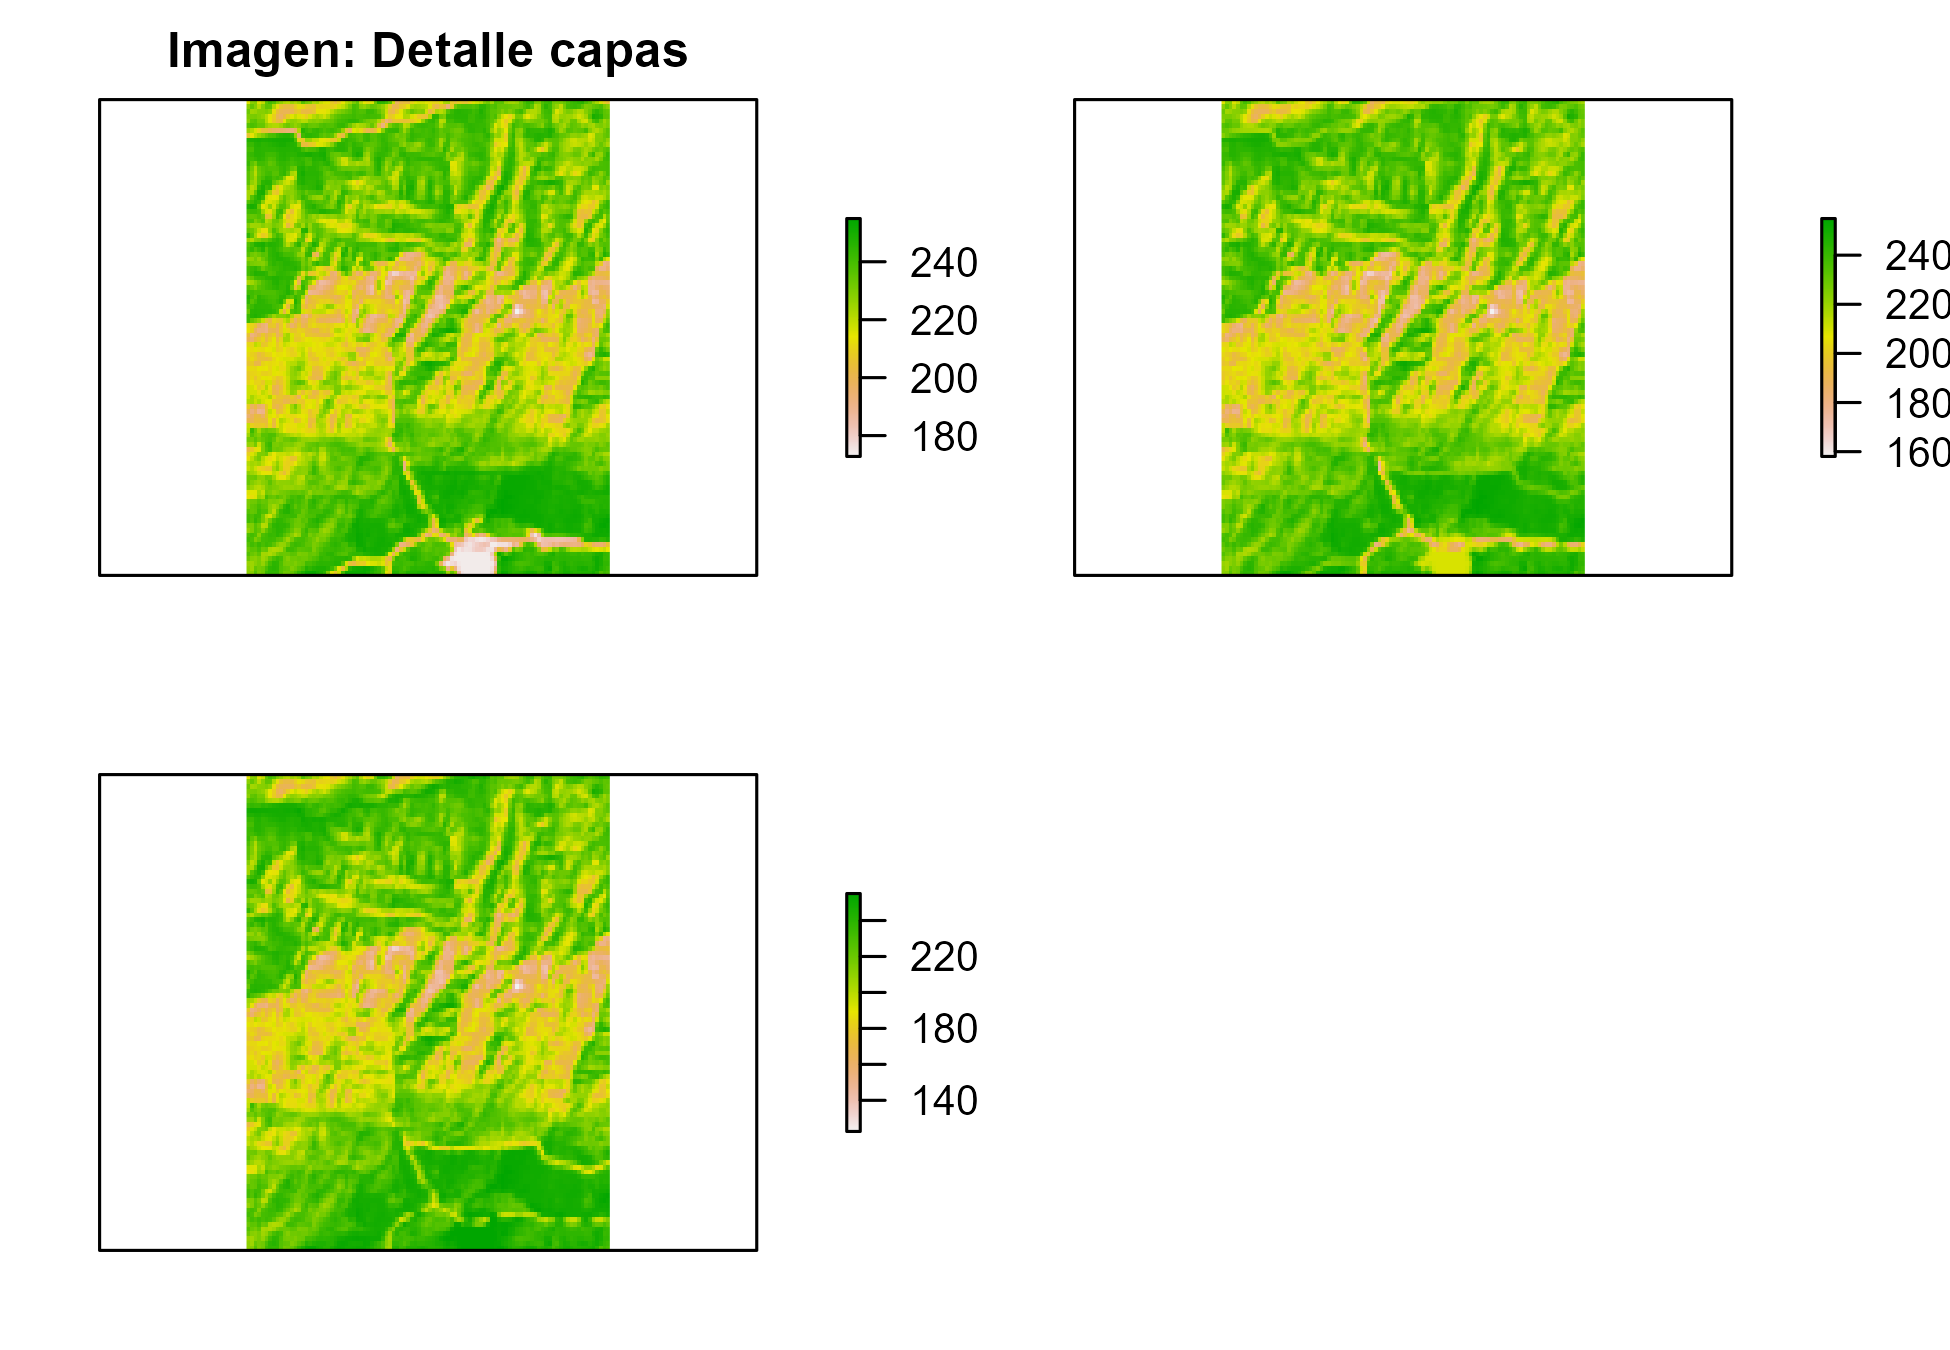
\includegraphics[width=0.6\linewidth]{_main_files/figure-latex/detalle-pixel-multicapa-2} 

}

\caption{Datos ráster multicapa: Descomposición}\label{fig:detalle-pixel-multicapa-2}
\end{figure}

\hypertarget{CRS}{%
\section{Sistema de Referencia de Coordenadas (CRS)}\label{CRS}}

Un sistema de referencia de coordenadas (o CRS por sus siglas en inglés,
\textbf{Coordinate Reference System}) permite relacionar datos espaciales con su
localización en la superficie terrestre.

\textbf{Los CRS constituyen por tanto un aspecto fundamental en el análisis y
representación de datos espaciales}, ya que nos permiten identificar con
exactitud la posición de los datos sobre el globo terráqueo.

Así mismo, cuando se trabaja con datos espaciales provenientes de distintas
fuentes de información, es necesario comprobar que dichos datos se encuentran
definidos en el mismo CRS:

\begin{figure}

{\centering 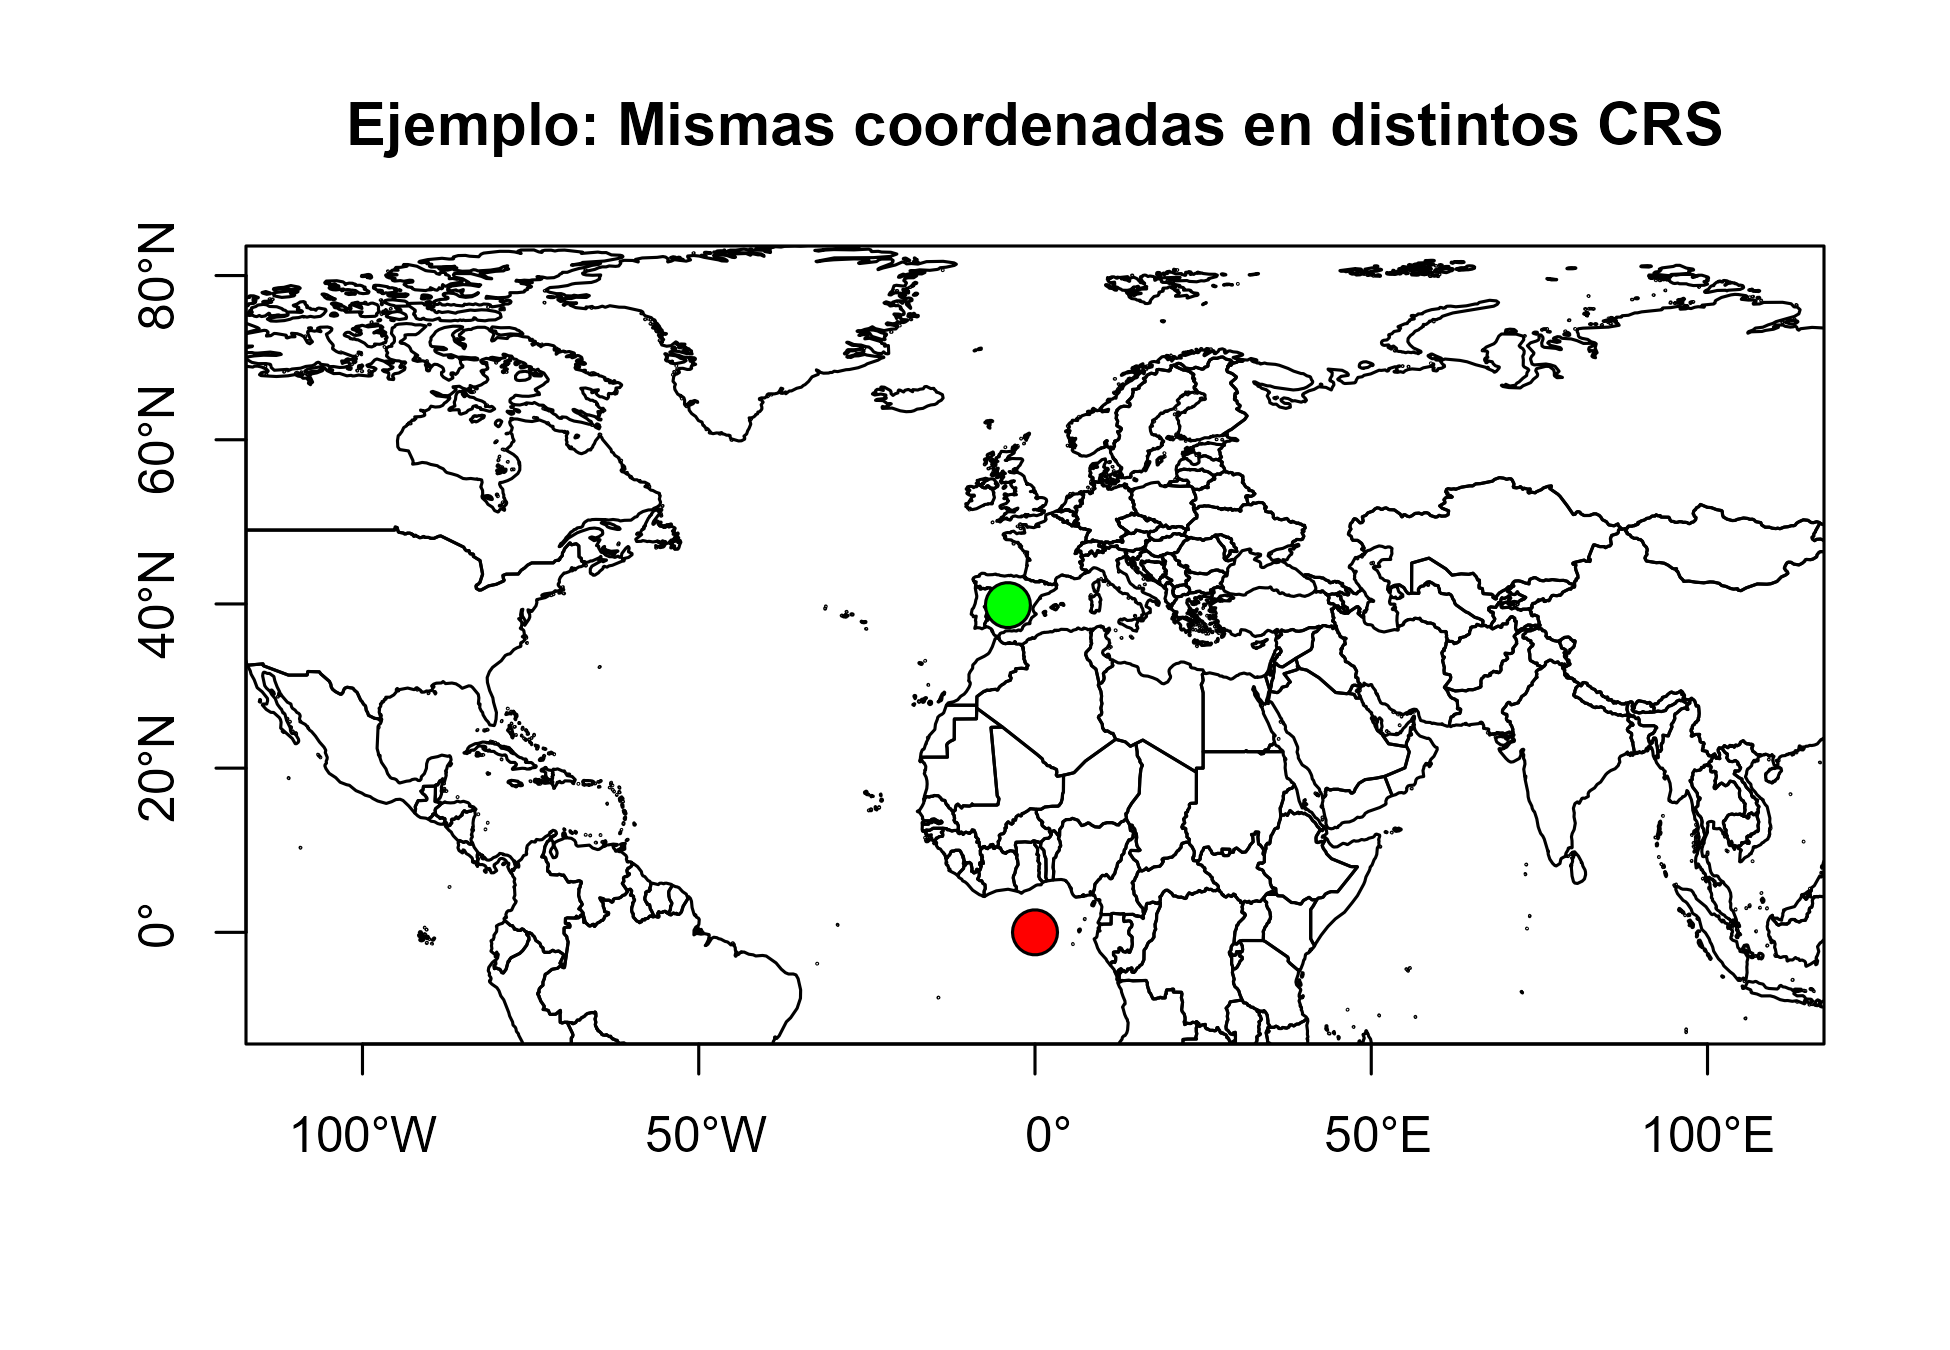
\includegraphics[width=0.6\linewidth]{_main_files/figure-latex/datosdesalineados-1} 

}

\caption{Representación de mismos valores de coordenadas en distintos CRS}\label{fig:datosdesalineados}
\end{figure}

En la Fig. \ref{fig:datosdesalineados}, ambos puntos (verde y rojo) tienen los
mismos valores de coordenadas en los ejes X e Y, en este caso las
correspondientes a la ciudad de Toledo. Sin embargo, presentan distintos CRS.
Por este motivo, al representar ambos puntos en un mapa, se observa que no se
están refiriendo a la misma localización geográfica. Esto es así porque el CRS
define la referencia (punto x=0 e y =0) y las unidades de los ejes (grados,
metros, millas).

Como conclusión, \textbf{además de disponer de las coordenadas de los datos
espaciales, es necesario conocer el CRS en el que están definidos para conocer
de manera exacta su localización geográfica.} Además, nótese que para cualquier
\textbf{análisis de datos espaciales} es necesario que todos los geodatos \textbf{se
encuentren referenciados en el mismo CRS}. Esto se consigue transformando (o
proyectando) los datos a un CRS común, nunca sobreescribiendo el CRS de los
mismos.

\hypertarget{tipos-de-crs}{%
\subsection{Tipos de CRS}\label{tipos-de-crs}}

A continuación se definen los dos grandes tipos de CRS, los CRS geográficos y
los CRS proyectados.

\hypertarget{crs-geogruxe1ficos}{%
\subsubsection{CRS geográficos}\label{crs-geogruxe1ficos}}

Los CRS geográficos son aquellos en los que los parámetros empleados para
localizar una posición espacial son la latitud y la longitud:

\begin{itemize}
\item
  \textbf{Latitud}: Es la distancia angular expresada en grados sobre el plano
  definido por el ecuador terrestre. Determina la posición sobre de una
  localización en el eje Norte-Sur de la Tierra y toma valores en el rango
  \([-90º,90º]\) . Las líneas imaginarias determinadas por una sucesión de
  puntos con la misma latitud a lo largo del eje Este-Oeste se denominan
  \textbf{paralelos} (Ver Fig. \ref{fig:meridianos}).
\item
  \textbf{Longitud}: Es la distancia angular expresada en grados sobre el plano
  definido por el meridiano de Greenwich. Determina la posición sobre de una
  localización en el eje Este-Oeste de la Tierra y toma valores en el rango
  \([-180º,180º]\) . Las líneas imaginarias determinadas por una sucesión de
  puntos con la misma longitud a lo largo del eje Este-Oeste se denominan
  \textbf{meridianos} (Ver Fig. \ref{fig:meridianos}).
\end{itemize}

\begin{figure}

{\centering 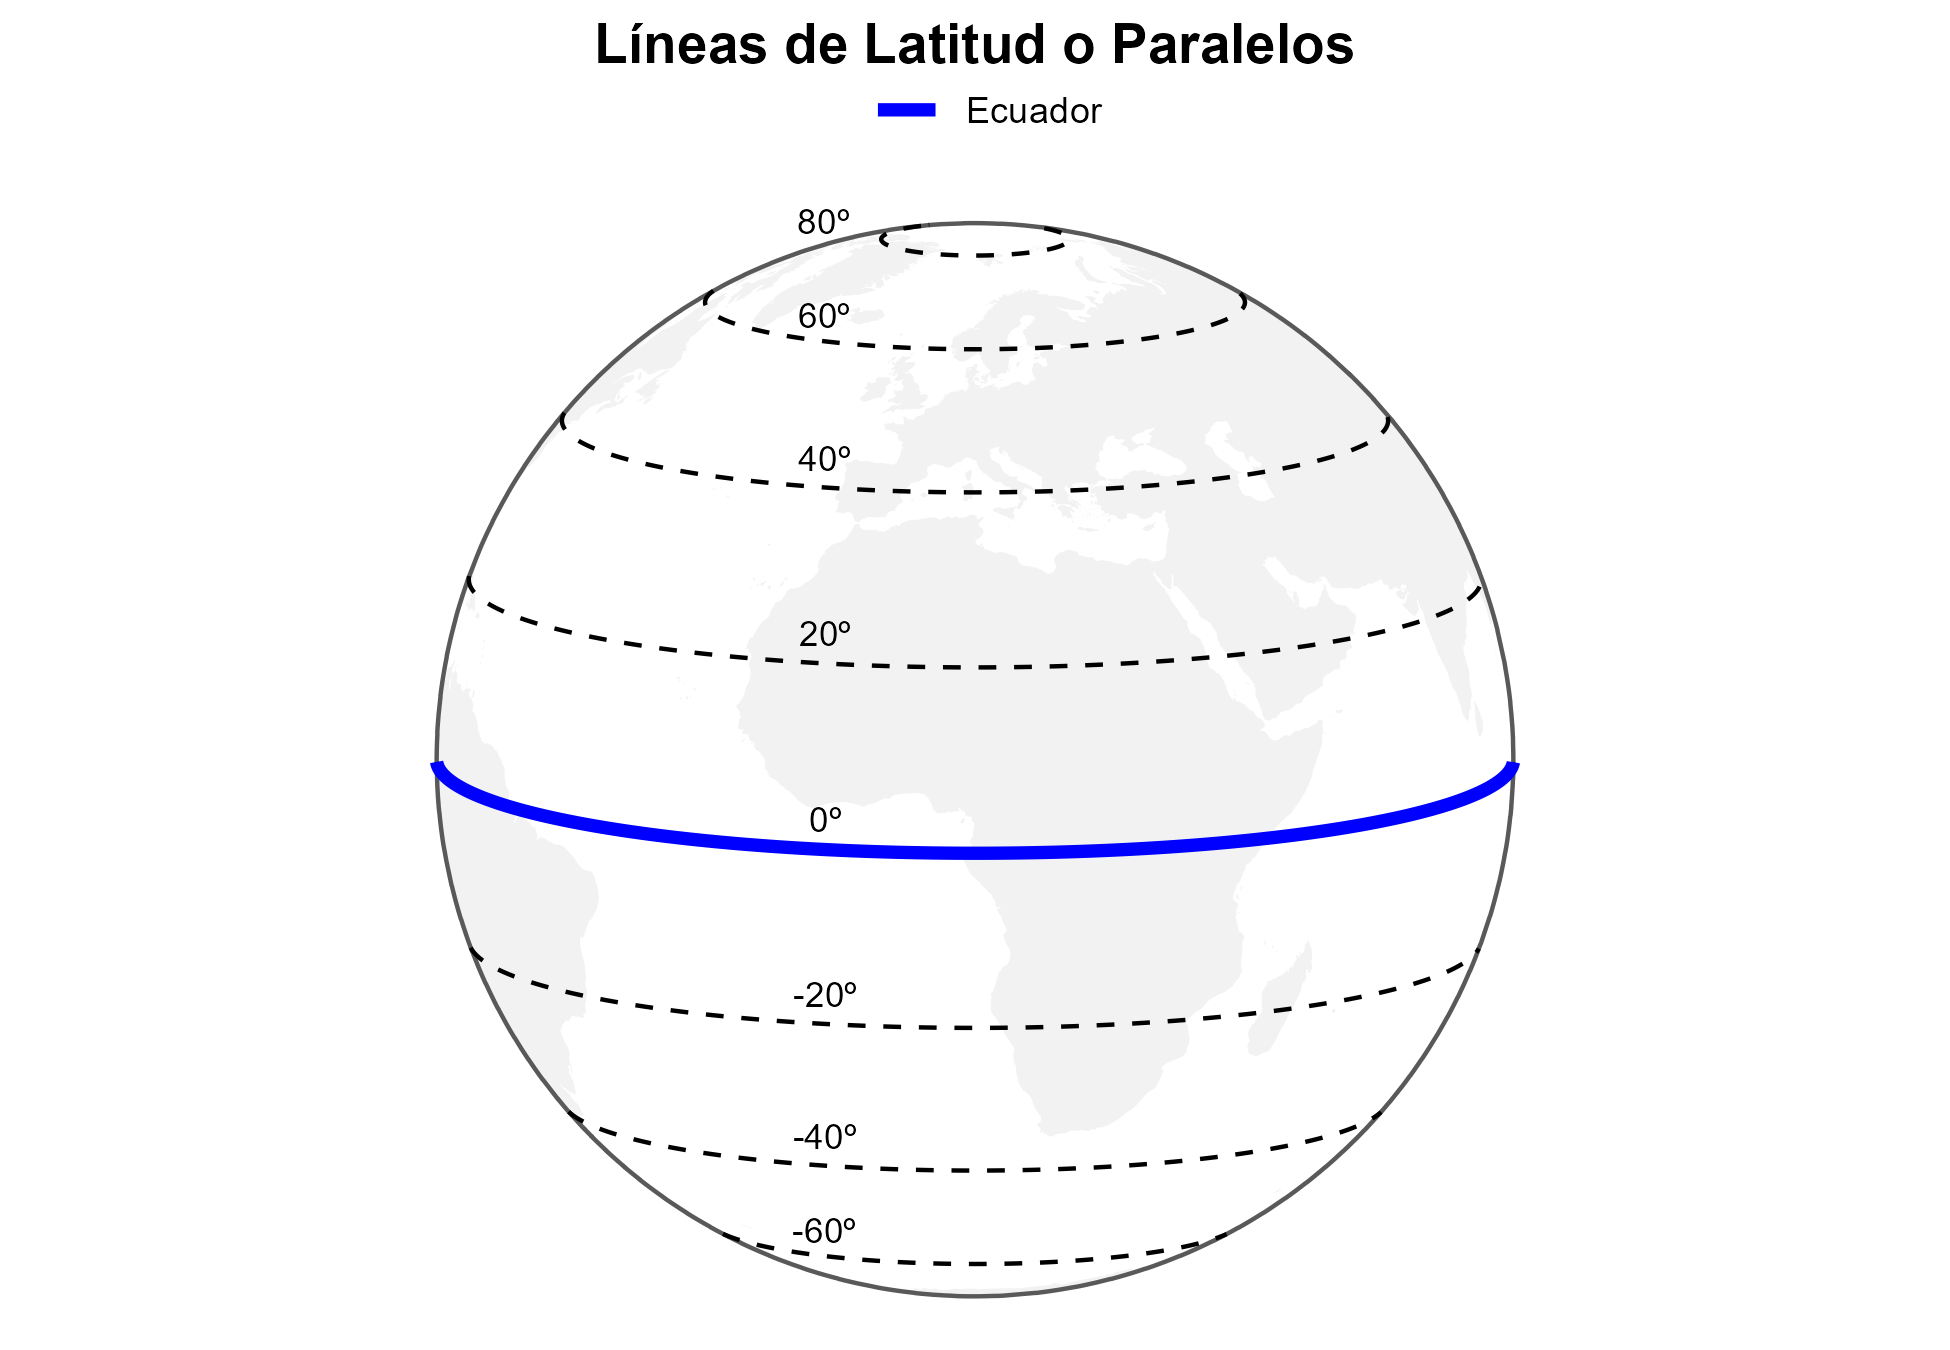
\includegraphics[width=0.5\linewidth]{_main_files/figure-latex/meridianos-1} 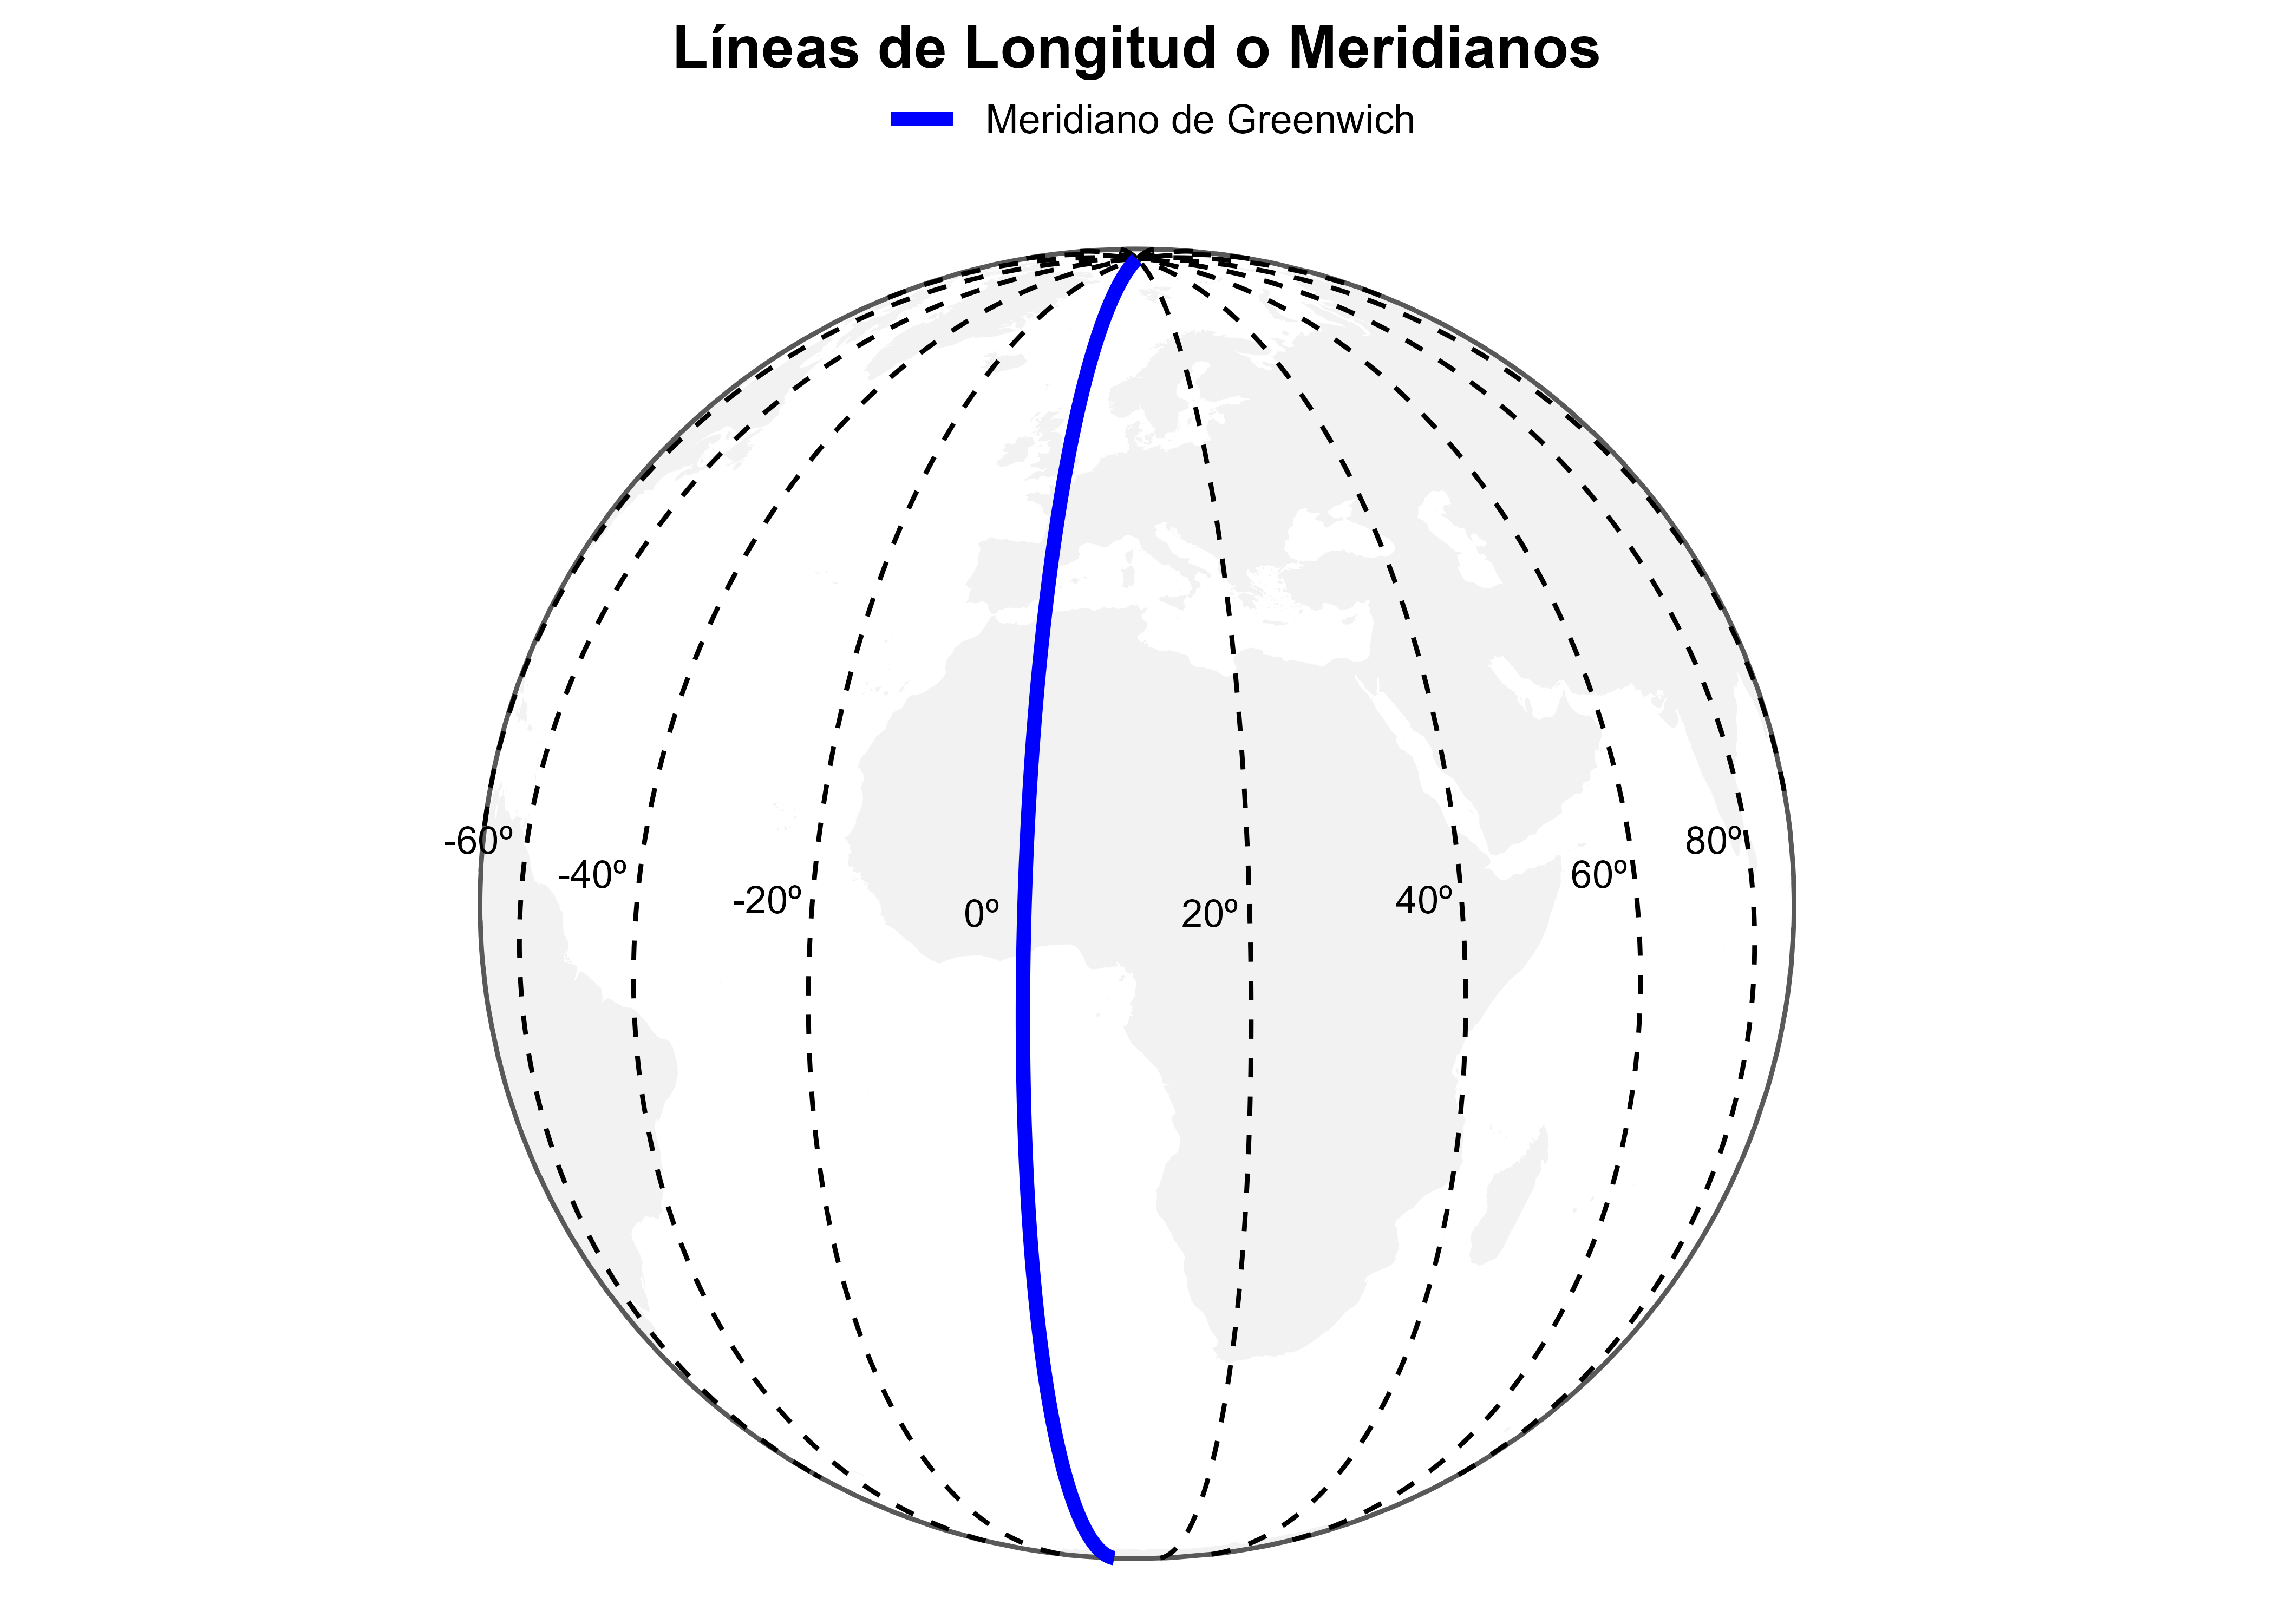
\includegraphics[width=0.5\linewidth]{_main_files/figure-latex/meridianos-2} 

}

\caption{Paralelos y Meridianos terrestres}\label{fig:meridianos}
\end{figure}

Es muy importante destacar que en un sistema de coordenadas geográfico, es
decir, basado en latitudes y longitudes, las \textbf{distancias} entre dos puntos
representan \textbf{distancias angulares}. Por ejemplo, la distancia entre el
meridiano de Greenwich y el meridiano correspondiente a la longitud 20º siempre
es de +20º. Sin embargo, debido a la forma esférica de la Tierra, la longitud en
metros entre ambos meridianos no es constante.

\begin{figure}

{\centering 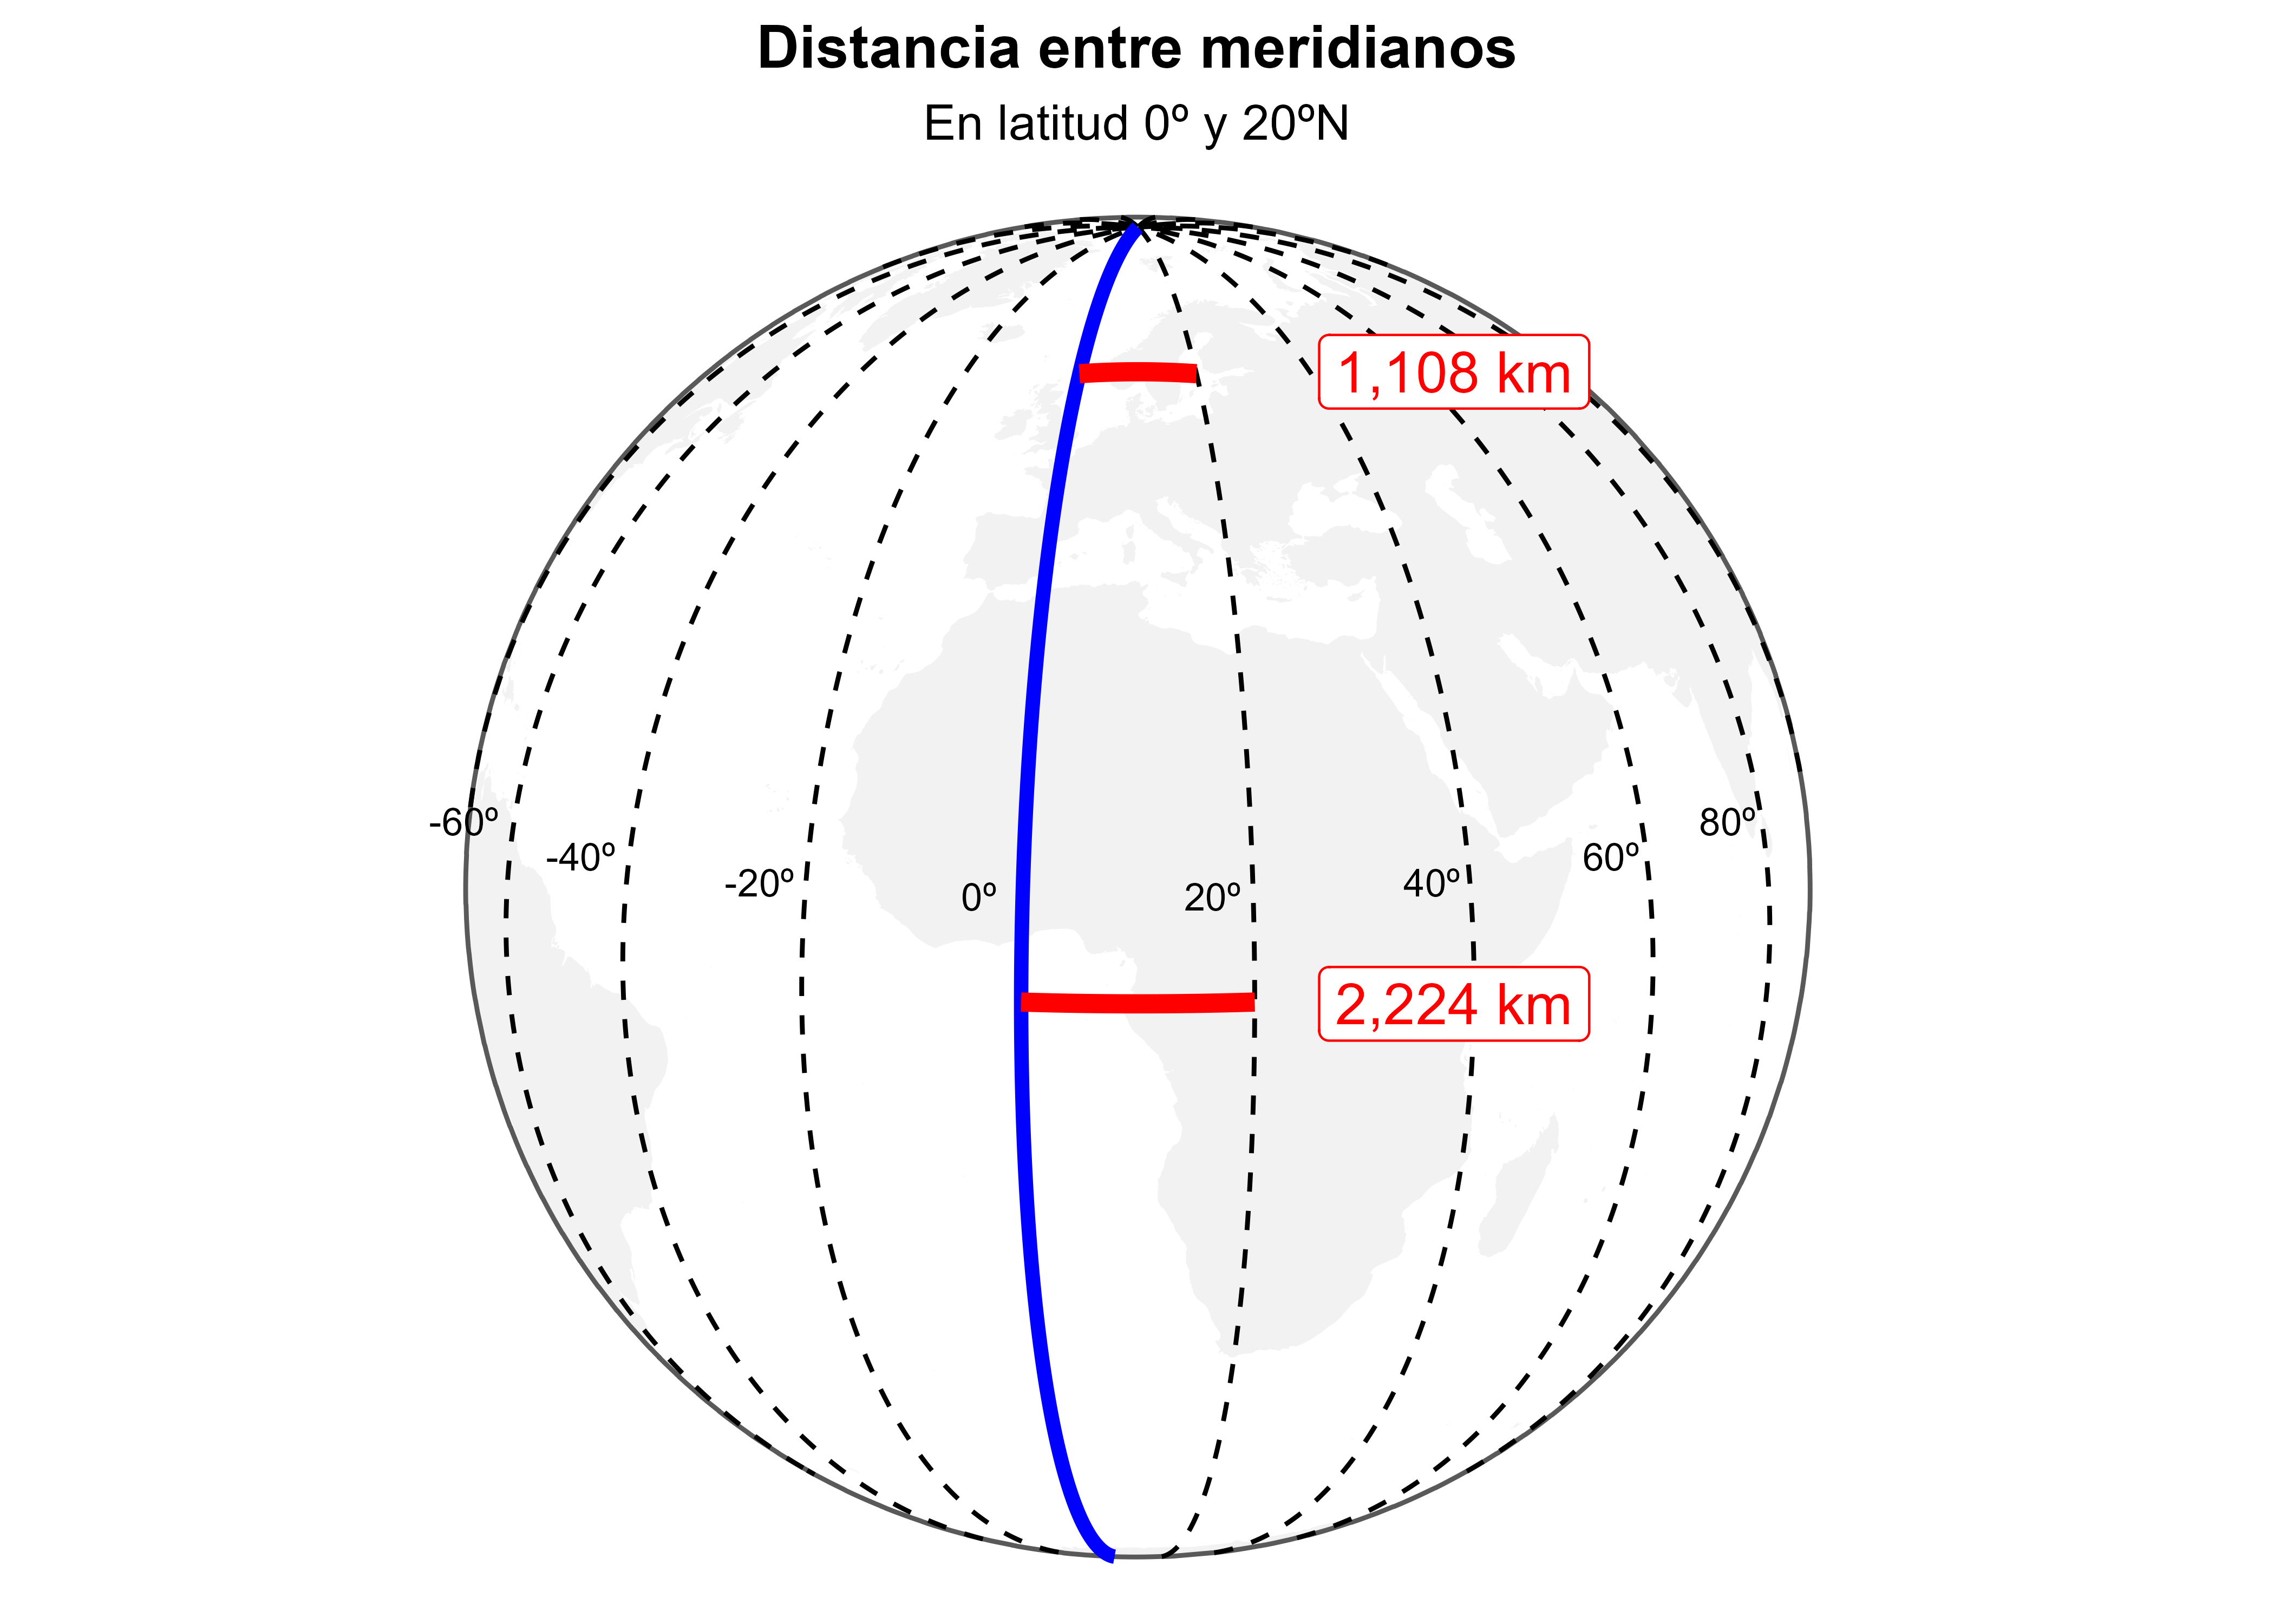
\includegraphics[width=0.6\linewidth]{_main_files/figure-latex/distang-1} 

}

\caption{Distancia entre meridianos en distintas latitudes}\label{fig:distang}
\end{figure}

\hypertarget{crs-proyectados}{%
\subsubsection{CRS proyectados}\label{crs-proyectados}}

La representación de formas tridimensionales en un soporte plano (dos
dimensiones) presenta algunos retos. Por ello, es habitual trabajar con
proyecciones de mapas.

Una \textbf{proyección geográfica} es un método para reducir la superficie de la
esfera terrestre a un sistema cartesiano de dos dimensiones. Para ello, es
necesario transformar las coordenadas longitud y latitud en coordenadas
cartesianas x e y.

Es importante destacar que las proyecciones pueden incluir un punto de origen
(X=0, Y=0) y unas unidades de distancia (habitualmente metros) específicas. Por
ejemplo, la \textbf{proyección cónica equiáreas de Albers} (específica para Estados
Unidos) define su punto de referencia (0,0) en la latitud 40º N y longitud 96º,
y la unidad de variación están definida en metros. De ahí la importancia de
conocer el CRS de los datos geográficos, como se expuso al principio de este
tema.

El Anexo \ref{crsproy} proporciona más información sobre los tipos de CRS
proyectados.

\hypertarget{trabajando-con-proyecciones-en-r}{%
\subsection{Trabajando con proyecciones en R}\label{trabajando-con-proyecciones-en-r}}

Existe toda una serie de proyecciones predefinidas, identificadas mediante los
\textbf{códigos EPSG, ESRI, WKT} o proj4 (en desuso en R, pero todavía admitidos).
Existen varios recursos web donde se pueden consultar y seleccionar los códigos
correspondientes:

\begin{itemize}
\item
  \url{https://epsg.io/}
\item
  \url{https://spatialreference.org/}
\item
  \url{https://proj.org/operations/projections/index.html}
\end{itemize}

Algunos de los códigos de proyecciones que es fundamental conocer son:

\begin{itemize}
\item
  \textbf{EPSG: 4326}: Proyección correspondiente a WGS 84, que es el sistema usado
  por los sistemas GPS. Cuando trabajemos con coordenadas geográficas
  longitud/latitud, este es habitualmente el CRS de referencia.
\item
  \textbf{EPSG: 3857}: Código correspondiente a la proyección de Mercator, usada
  habitualmente por servicios como Google Maps, etc.
\end{itemize}

Se pueden consultar otros CRS de uso común en España en la página del
\href{https://www.mapa.gob.es/es/cartografia-y-sig/ide/directorio_datos_servicios/caracteristicas_wms.aspx}{Ministerio de Agricultura, Pesca y
Alimentación}

En la sección \ref{quecrsuso} veremos cómo encontrar un CRS usando el paquete
\texttt{crsuggest}.

El paquete \texttt{sf} permite obtener los parámetros de cualquier proyección mediante
la función \texttt{st\_crs()}:

\textbf{(i) EPSG WGS 84 (Sistema Global GPS): EPSG 4326}

\begin{Shaded}
\begin{Highlighting}[]
\FunctionTok{library}\NormalTok{(sf)}

\CommentTok{\# Ejemplo: EPSG WGS 84 (Sistema Global GPS): EPSG 4326}
\FunctionTok{st\_crs}\NormalTok{(}\DecValTok{4326}\NormalTok{)}
\CommentTok{\#\textgreater{} Coordinate Reference System:}
\CommentTok{\#\textgreater{}   User input: EPSG:4326 }
\CommentTok{\#\textgreater{}   wkt:}
\CommentTok{\#\textgreater{} GEOGCRS["WGS 84",}
\CommentTok{\#\textgreater{}     DATUM["World Geodetic System 1984",}
\CommentTok{\#\textgreater{}         ELLIPSOID["WGS 84",6378137,298.257223563,}
\CommentTok{\#\textgreater{}             LENGTHUNIT["metre",1]]],}
\CommentTok{\#\textgreater{}     PRIMEM["Greenwich",0,}
\CommentTok{\#\textgreater{}         ANGLEUNIT["degree",0.0174532925199433]],}
\CommentTok{\#\textgreater{}     CS[ellipsoidal,2],}
\CommentTok{\#\textgreater{}         AXIS["geodetic latitude (Lat)",north,}
\CommentTok{\#\textgreater{}             ORDER[1],}
\CommentTok{\#\textgreater{}             ANGLEUNIT["degree",0.0174532925199433]],}
\CommentTok{\#\textgreater{}         AXIS["geodetic longitude (Lon)",east,}
\CommentTok{\#\textgreater{}             ORDER[2],}
\CommentTok{\#\textgreater{}             ANGLEUNIT["degree",0.0174532925199433]],}
\CommentTok{\#\textgreater{}     USAGE[}
\CommentTok{\#\textgreater{}         SCOPE["Horizontal component of 3D system."],}
\CommentTok{\#\textgreater{}         AREA["World."],}
\CommentTok{\#\textgreater{}         BBOX[{-}90,{-}180,90,180]],}
\CommentTok{\#\textgreater{}     ID["EPSG",4326]]}
\end{Highlighting}
\end{Shaded}

\textbf{(ii) ESRI North America Albers Equal Area Conic: ESRI:102008}

\begin{Shaded}
\begin{Highlighting}[]
\CommentTok{\# Usando código ESRI North America Albers Equal Area Conic}

\FunctionTok{st\_crs}\NormalTok{(}\StringTok{"ESRI:102008"}\NormalTok{)}
\CommentTok{\#\textgreater{} Coordinate Reference System:}
\CommentTok{\#\textgreater{}   User input: ESRI:102008 }
\CommentTok{\#\textgreater{}   wkt:}
\CommentTok{\#\textgreater{} PROJCRS["North\_America\_Albers\_Equal\_Area\_Conic",}
\CommentTok{\#\textgreater{}     BASEGEOGCRS["NAD83",}
\CommentTok{\#\textgreater{}         DATUM["North American Datum 1983",}
\CommentTok{\#\textgreater{}             ELLIPSOID["GRS 1980",6378137,298.257222101,}
\CommentTok{\#\textgreater{}                 LENGTHUNIT["metre",1]]],}
\CommentTok{\#\textgreater{}         PRIMEM["Greenwich",0,}
\CommentTok{\#\textgreater{}             ANGLEUNIT["Degree",0.0174532925199433]]],}
\CommentTok{\#\textgreater{}     CONVERSION["North\_America\_Albers\_Equal\_Area\_Conic",}
\CommentTok{\#\textgreater{}         METHOD["Albers Equal Area",}
\CommentTok{\#\textgreater{}             ID["EPSG",9822]],}
\CommentTok{\#\textgreater{}         PARAMETER["Latitude of false origin",40,}
\CommentTok{\#\textgreater{}             ANGLEUNIT["Degree",0.0174532925199433],}
\CommentTok{\#\textgreater{}             ID["EPSG",8821]],}
\CommentTok{\#\textgreater{}         PARAMETER["Longitude of false origin",{-}96,}
\CommentTok{\#\textgreater{}             ANGLEUNIT["Degree",0.0174532925199433],}
\CommentTok{\#\textgreater{}             ID["EPSG",8822]],}
\CommentTok{\#\textgreater{}         PARAMETER["Latitude of 1st standard parallel",20,}
\CommentTok{\#\textgreater{}             ANGLEUNIT["Degree",0.0174532925199433],}
\CommentTok{\#\textgreater{}             ID["EPSG",8823]],}
\CommentTok{\#\textgreater{}         PARAMETER["Latitude of 2nd standard parallel",60,}
\CommentTok{\#\textgreater{}             ANGLEUNIT["Degree",0.0174532925199433],}
\CommentTok{\#\textgreater{}             ID["EPSG",8824]],}
\CommentTok{\#\textgreater{}         PARAMETER["Easting at false origin",0,}
\CommentTok{\#\textgreater{}             LENGTHUNIT["metre",1],}
\CommentTok{\#\textgreater{}             ID["EPSG",8826]],}
\CommentTok{\#\textgreater{}         PARAMETER["Northing at false origin",0,}
\CommentTok{\#\textgreater{}             LENGTHUNIT["metre",1],}
\CommentTok{\#\textgreater{}             ID["EPSG",8827]]],}
\CommentTok{\#\textgreater{}     CS[Cartesian,2],}
\CommentTok{\#\textgreater{}         AXIS["(E)",east,}
\CommentTok{\#\textgreater{}             ORDER[1],}
\CommentTok{\#\textgreater{}             LENGTHUNIT["metre",1]],}
\CommentTok{\#\textgreater{}         AXIS["(N)",north,}
\CommentTok{\#\textgreater{}             ORDER[2],}
\CommentTok{\#\textgreater{}             LENGTHUNIT["metre",1]],}
\CommentTok{\#\textgreater{}     USAGE[}
\CommentTok{\#\textgreater{}         SCOPE["Not known."],}
\CommentTok{\#\textgreater{}         AREA["North America {-} onshore and offshore: Canada {-} Alberta; British Columbia; Manitoba; New Brunswick; Newfoundland and Labrador; Northwest Territories; Nova Scotia; Nunavut; Ontario; Prince Edward Island; Quebec; Saskatchewan; Yukon. United States (USA) {-} Alabama; Alaska (mainland); Arizona; Arkansas; California; Colorado; Connecticut; Delaware; Florida; Georgia; Idaho; Illinois; Indiana; Iowa; Kansas; Kentucky; Louisiana; Maine; Maryland; Massachusetts; Michigan; Minnesota; Mississippi; Missouri; Montana; Nebraska; Nevada; New Hampshire; New Jersey; New Mexico; New York; North Carolina; North Dakota; Ohio; Oklahoma; Oregon; Pennsylvania; Rhode Island; South Carolina; South Dakota; Tennessee; Texas; Utah; Vermont; Virginia; Washington; West Virginia; Wisconsin; Wyoming."],}
\CommentTok{\#\textgreater{}         BBOX[23.81,{-}172.54,86.46,{-}47.74]],}
\CommentTok{\#\textgreater{}     ID["ESRI",102008]]}
\end{Highlighting}
\end{Shaded}

\textbf{(iii) Usando proj4string: Robinson: +proj=robin}

\begin{Shaded}
\begin{Highlighting}[]
\CommentTok{\# Usando proj4string: Robinson}

\FunctionTok{st\_crs}\NormalTok{(}\StringTok{"+proj=robin"}\NormalTok{)}
\CommentTok{\#\textgreater{} Coordinate Reference System:}
\CommentTok{\#\textgreater{}   User input: +proj=robin }
\CommentTok{\#\textgreater{}   wkt:}
\CommentTok{\#\textgreater{} PROJCRS["unknown",}
\CommentTok{\#\textgreater{}     BASEGEOGCRS["unknown",}
\CommentTok{\#\textgreater{}         DATUM["World Geodetic System 1984",}
\CommentTok{\#\textgreater{}             ELLIPSOID["WGS 84",6378137,298.257223563,}
\CommentTok{\#\textgreater{}                 LENGTHUNIT["metre",1]],}
\CommentTok{\#\textgreater{}             ID["EPSG",6326]],}
\CommentTok{\#\textgreater{}         PRIMEM["Greenwich",0,}
\CommentTok{\#\textgreater{}             ANGLEUNIT["degree",0.0174532925199433],}
\CommentTok{\#\textgreater{}             ID["EPSG",8901]]],}
\CommentTok{\#\textgreater{}     CONVERSION["unknown",}
\CommentTok{\#\textgreater{}         METHOD["Robinson"],}
\CommentTok{\#\textgreater{}         PARAMETER["Longitude of natural origin",0,}
\CommentTok{\#\textgreater{}             ANGLEUNIT["degree",0.0174532925199433],}
\CommentTok{\#\textgreater{}             ID["EPSG",8802]],}
\CommentTok{\#\textgreater{}         PARAMETER["False easting",0,}
\CommentTok{\#\textgreater{}             LENGTHUNIT["metre",1],}
\CommentTok{\#\textgreater{}             ID["EPSG",8806]],}
\CommentTok{\#\textgreater{}         PARAMETER["False northing",0,}
\CommentTok{\#\textgreater{}             LENGTHUNIT["metre",1],}
\CommentTok{\#\textgreater{}             ID["EPSG",8807]]],}
\CommentTok{\#\textgreater{}     CS[Cartesian,2],}
\CommentTok{\#\textgreater{}         AXIS["(E)",east,}
\CommentTok{\#\textgreater{}             ORDER[1],}
\CommentTok{\#\textgreater{}             LENGTHUNIT["metre",1,}
\CommentTok{\#\textgreater{}                 ID["EPSG",9001]]],}
\CommentTok{\#\textgreater{}         AXIS["(N)",north,}
\CommentTok{\#\textgreater{}             ORDER[2],}
\CommentTok{\#\textgreater{}             LENGTHUNIT["metre",1,}
\CommentTok{\#\textgreater{}                 ID["EPSG",9001]]]]}
\end{Highlighting}
\end{Shaded}

La mayoría de los objetos espaciales serán de la clase \texttt{sf}, por tanto, resulta
interesante conocer cómo se proyectan estos objetos.

Es posible proyectar un objeto \texttt{sf} mediante la función \texttt{st\_transform()}. En el
siguiente ejemplo vemos cómo partimos de un objeto con \textbf{EPSG:4326} y cambiamos
su proyección a otras proyecciones, como \textbf{Mercator} o \textbf{Robinson}:

\begin{Shaded}
\begin{Highlighting}[]

\CommentTok{\# Usa datos del paquete giscoR}

\FunctionTok{library}\NormalTok{(giscoR)}

\NormalTok{paises }\OtherTok{\textless{}{-}} \FunctionTok{gisco\_get\_countries}\NormalTok{()}

\CommentTok{\# Comprobamos el CRS de estos datos}
\CommentTok{\# Se puede almacenar en un objeto y usar posteriormente}
\CommentTok{\# Vemos que es EPSG:4326, por tanto son coordenadas geográficas longitud/latitud}
\FunctionTok{st\_crs}\NormalTok{(paises)}
\CommentTok{\#\textgreater{} Coordinate Reference System:}
\CommentTok{\#\textgreater{}   User input: EPSG:4326 }
\CommentTok{\#\textgreater{}   wkt:}
\CommentTok{\#\textgreater{} GEOGCS["WGS 84",}
\CommentTok{\#\textgreater{}     DATUM["WGS\_1984",}
\CommentTok{\#\textgreater{}         SPHEROID["WGS 84",6378137,298.257223563,}
\CommentTok{\#\textgreater{}             AUTHORITY["EPSG","7030"]],}
\CommentTok{\#\textgreater{}         AUTHORITY["EPSG","6326"]],}
\CommentTok{\#\textgreater{}     PRIMEM["Greenwich",0,}
\CommentTok{\#\textgreater{}         AUTHORITY["EPSG","8901"]],}
\CommentTok{\#\textgreater{}     UNIT["degree",0.0174532925199433,}
\CommentTok{\#\textgreater{}         AUTHORITY["EPSG","9122"]],}
\CommentTok{\#\textgreater{}     AUTHORITY["EPSG","4326"]]}

\CommentTok{\# Plot}
\FunctionTok{plot}\NormalTok{(}\FunctionTok{st\_geometry}\NormalTok{(paises), }\AttributeTok{axes =} \ConstantTok{TRUE}\NormalTok{)}
\end{Highlighting}
\end{Shaded}

\begin{figure}

{\centering 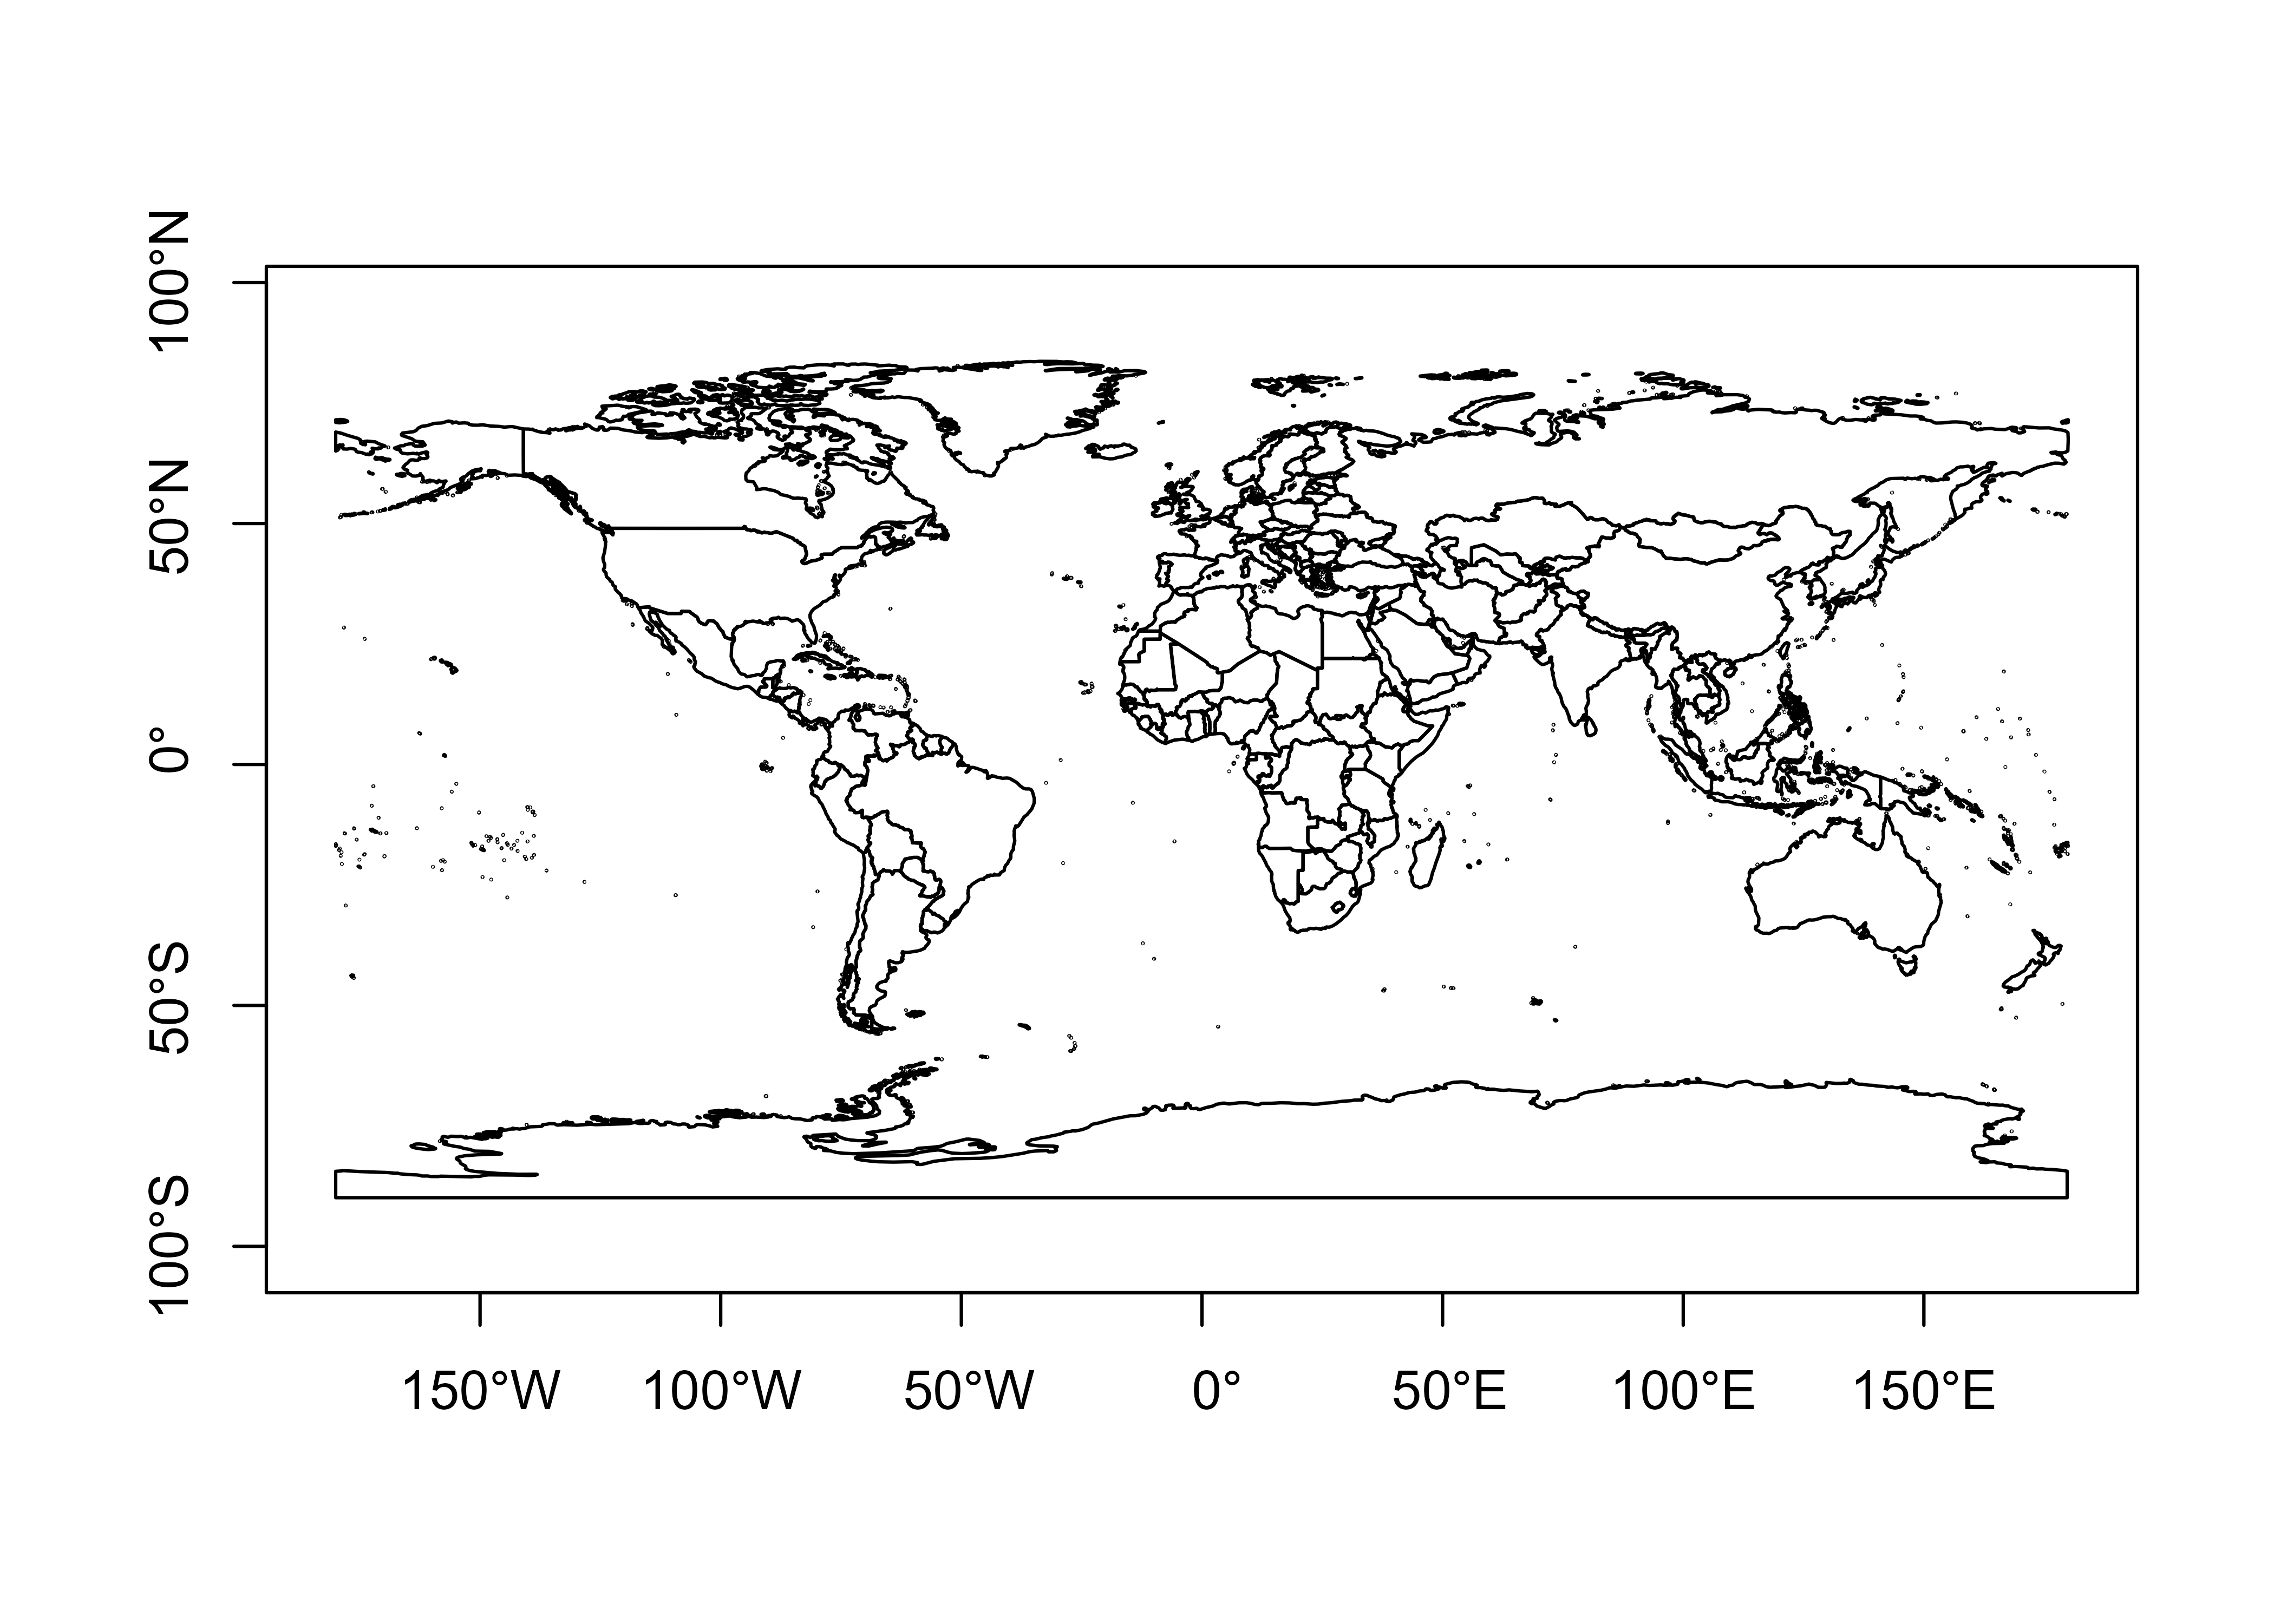
\includegraphics[width=0.6\linewidth]{_main_files/figure-latex/project-map-1} 

}

\caption{Proyección del mundo en coordenadas geográficas (EPSG 4326)}\label{fig:project-map-1}
\end{figure}

\begin{Shaded}
\begin{Highlighting}[]

\CommentTok{\# Proyectamos a Mercator}
\CommentTok{\# El eje cambia porque Mercator usa metros}
\NormalTok{paises\_merc }\OtherTok{\textless{}{-}} \FunctionTok{st\_transform}\NormalTok{(paises, }\FunctionTok{st\_crs}\NormalTok{(}\DecValTok{3857}\NormalTok{))}
\FunctionTok{plot}\NormalTok{(}\FunctionTok{st\_geometry}\NormalTok{(paises\_merc), }\AttributeTok{axes =} \ConstantTok{TRUE}\NormalTok{)}
\end{Highlighting}
\end{Shaded}

\begin{figure}

{\centering 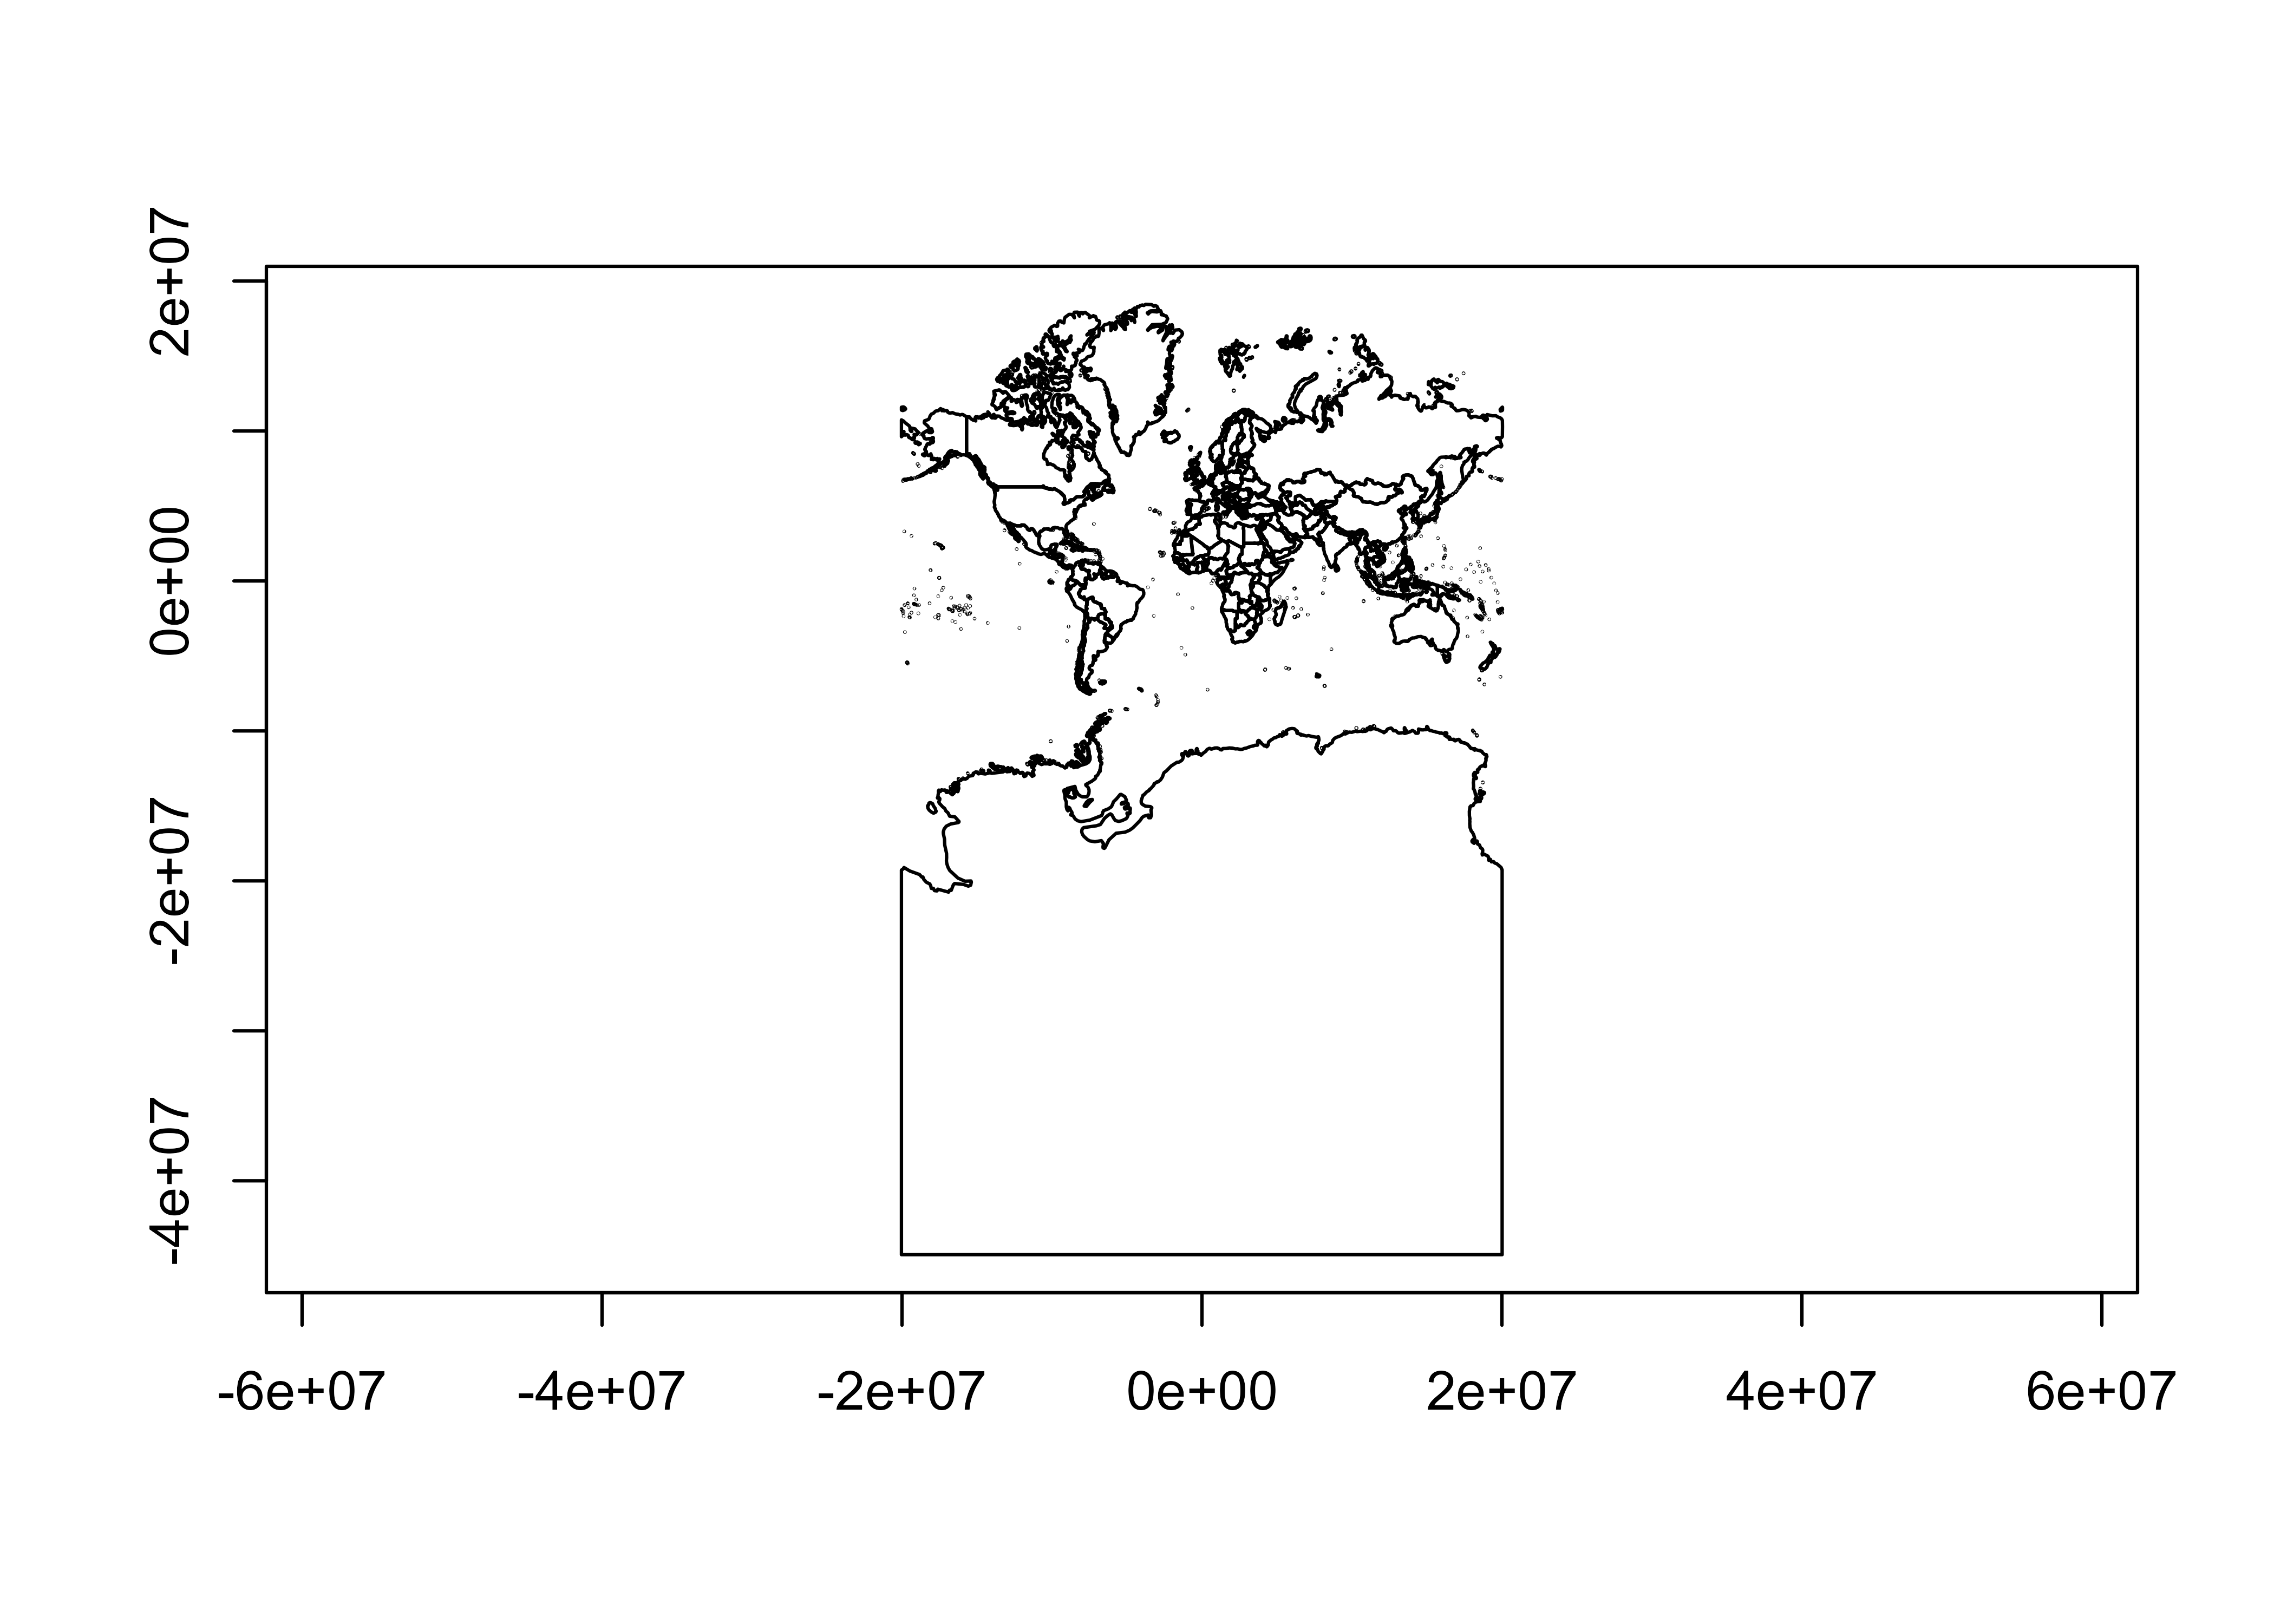
\includegraphics[width=0.6\linewidth]{_main_files/figure-latex/project-map-2} 

}

\caption{Proyección del mundo en Mercator (EPSG 3857)}\label{fig:project-map-2}
\end{figure}

\begin{Shaded}
\begin{Highlighting}[]
\CommentTok{\# Proyectamos a Robinson}
\NormalTok{paises\_robin }\OtherTok{\textless{}{-}} \FunctionTok{st\_transform}\NormalTok{(paises, }\FunctionTok{st\_crs}\NormalTok{(}\StringTok{"+proj=robin"}\NormalTok{))}
\FunctionTok{plot}\NormalTok{(}\FunctionTok{st\_geometry}\NormalTok{(paises\_robin), }\AttributeTok{axes =} \ConstantTok{TRUE}\NormalTok{)}
\end{Highlighting}
\end{Shaded}

\begin{figure}

{\centering 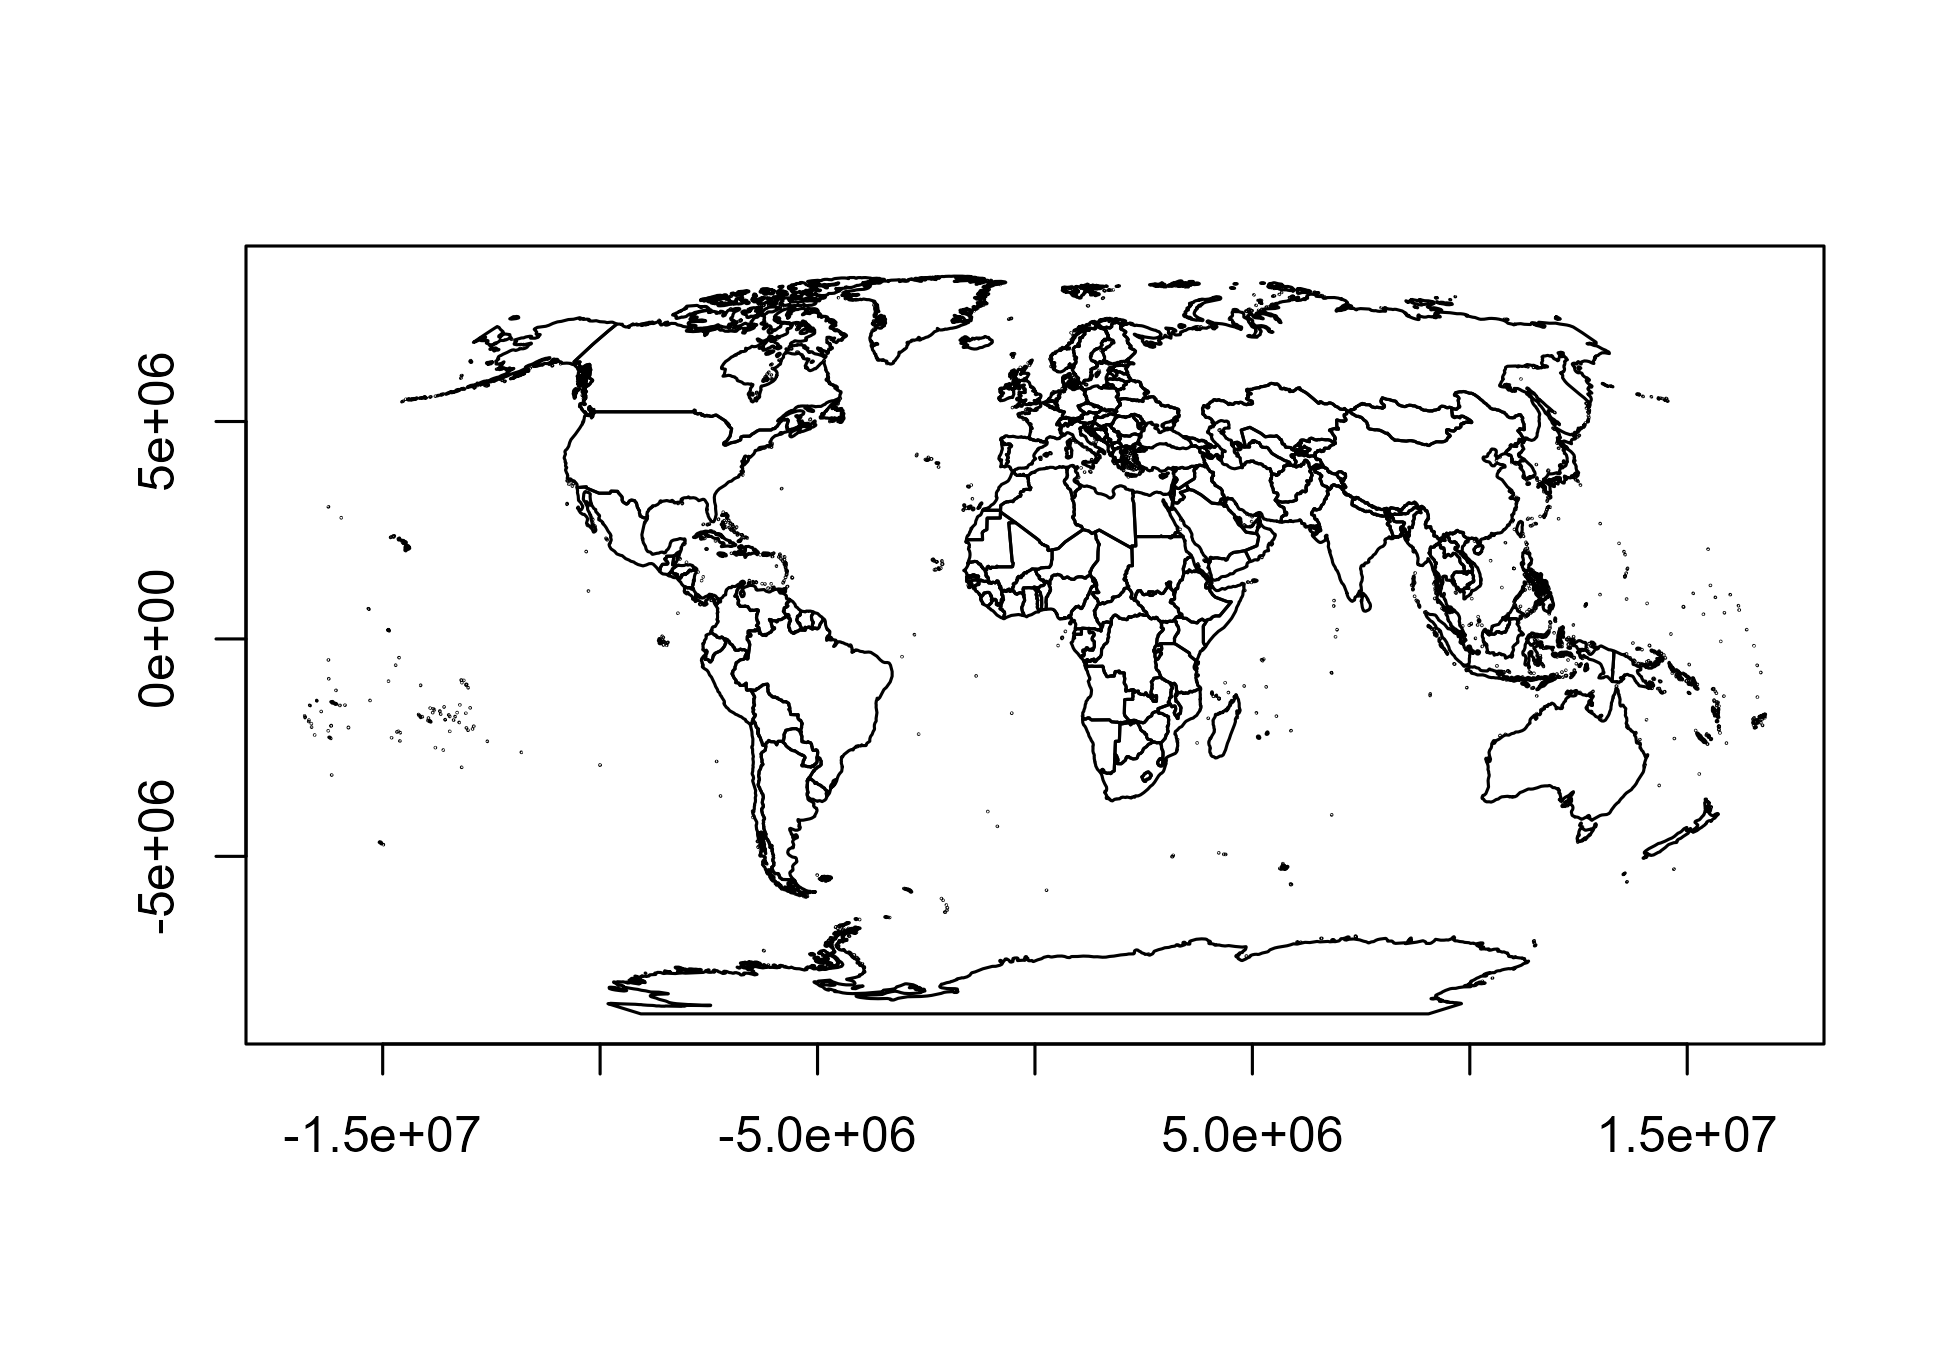
\includegraphics[width=0.6\linewidth]{_main_files/figure-latex/project-map-3} 

}

\caption{Proyección del mundo en Robinson (+proj=robin)}\label{fig:project-map-3}
\end{figure}

Como se comentó anteriormente, cuando se usan geodatos de diversas fuentes, es
necesario que todos presenten el mismo CRS. En la Fig \ref{fig:puertos-error}
se muestra lo que ocurre si esto no se cumple:

\begin{Shaded}
\begin{Highlighting}[]
\CommentTok{\# Añadimos a este mapa puertos mundiales de giscoR}

\NormalTok{puertos }\OtherTok{\textless{}{-}} \FunctionTok{gisco\_get\_ports}\NormalTok{()}
\FunctionTok{plot}\NormalTok{(}\FunctionTok{st\_geometry}\NormalTok{(paises\_robin), }\AttributeTok{main =} \StringTok{"Puertos en el mundo"}\NormalTok{)}
\FunctionTok{plot}\NormalTok{(}\FunctionTok{st\_geometry}\NormalTok{(puertos), }\AttributeTok{add =} \ConstantTok{TRUE}\NormalTok{, }\AttributeTok{col =} \StringTok{"red"}\NormalTok{, }\AttributeTok{pch =} \DecValTok{20}\NormalTok{)}
\end{Highlighting}
\end{Shaded}

\begin{figure}

{\centering 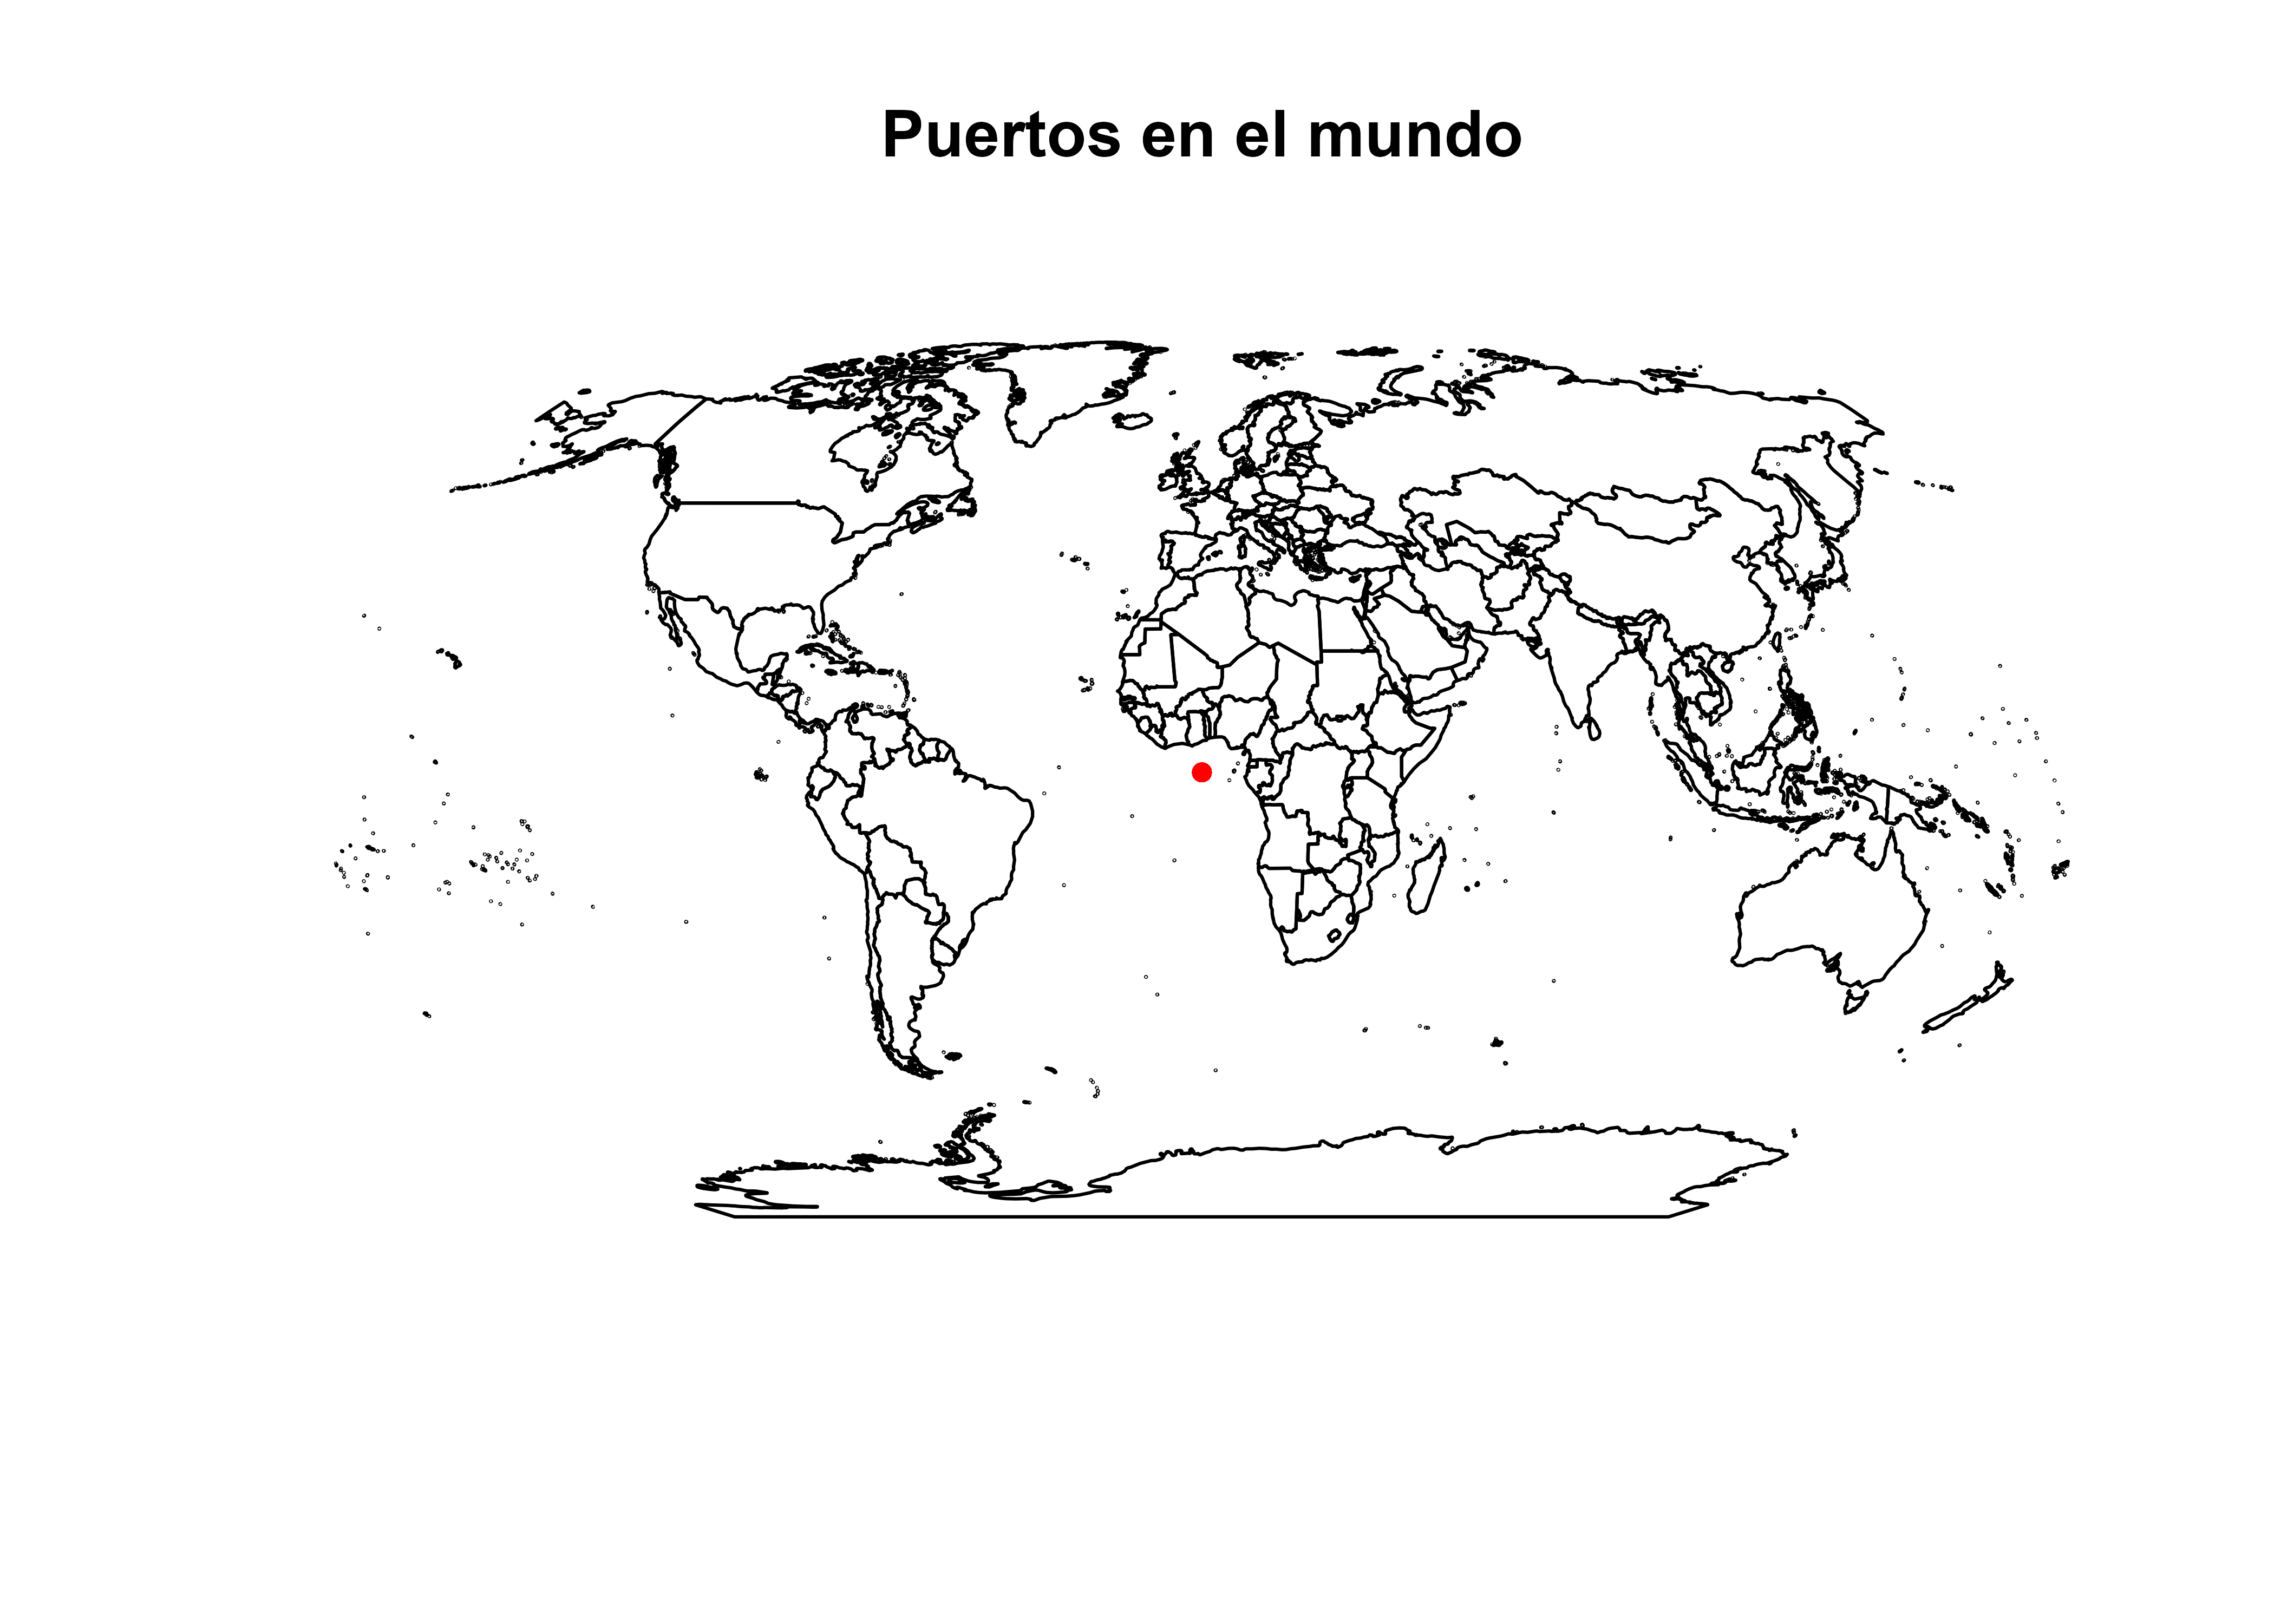
\includegraphics[width=0.6\linewidth]{_main_files/figure-latex/puertos-error-1} 

}

\caption{Ejemplo: Puertos del mundo}\label{fig:puertos-error}
\end{figure}

Vemos que ha habido algún tipo de error, ¿a que puede deberse?

\begin{Shaded}
\begin{Highlighting}[]
\CommentTok{\# Comprueba CRS}

\FunctionTok{st\_crs}\NormalTok{(puertos) }\SpecialCharTok{==} \FunctionTok{st\_crs}\NormalTok{(paises\_robin)}
\CommentTok{\#\textgreater{} [1] FALSE}

\CommentTok{\# Los puertos no están en Robinson! Proyectamos al mismo CRS}
\NormalTok{puertos\_robin }\OtherTok{\textless{}{-}} \FunctionTok{st\_transform}\NormalTok{(puertos, }\FunctionTok{st\_crs}\NormalTok{(paises\_robin))}
\FunctionTok{plot}\NormalTok{(}\FunctionTok{st\_geometry}\NormalTok{(paises\_robin), }\AttributeTok{main =} \StringTok{"Puertos en el mundo"}\NormalTok{)}
\FunctionTok{plot}\NormalTok{(}\FunctionTok{st\_geometry}\NormalTok{(puertos\_robin), }\AttributeTok{add =} \ConstantTok{TRUE}\NormalTok{, }\AttributeTok{col =} \StringTok{"blue"}\NormalTok{, }\AttributeTok{pch =} \DecValTok{20}\NormalTok{)}
\end{Highlighting}
\end{Shaded}

\begin{figure}

{\centering 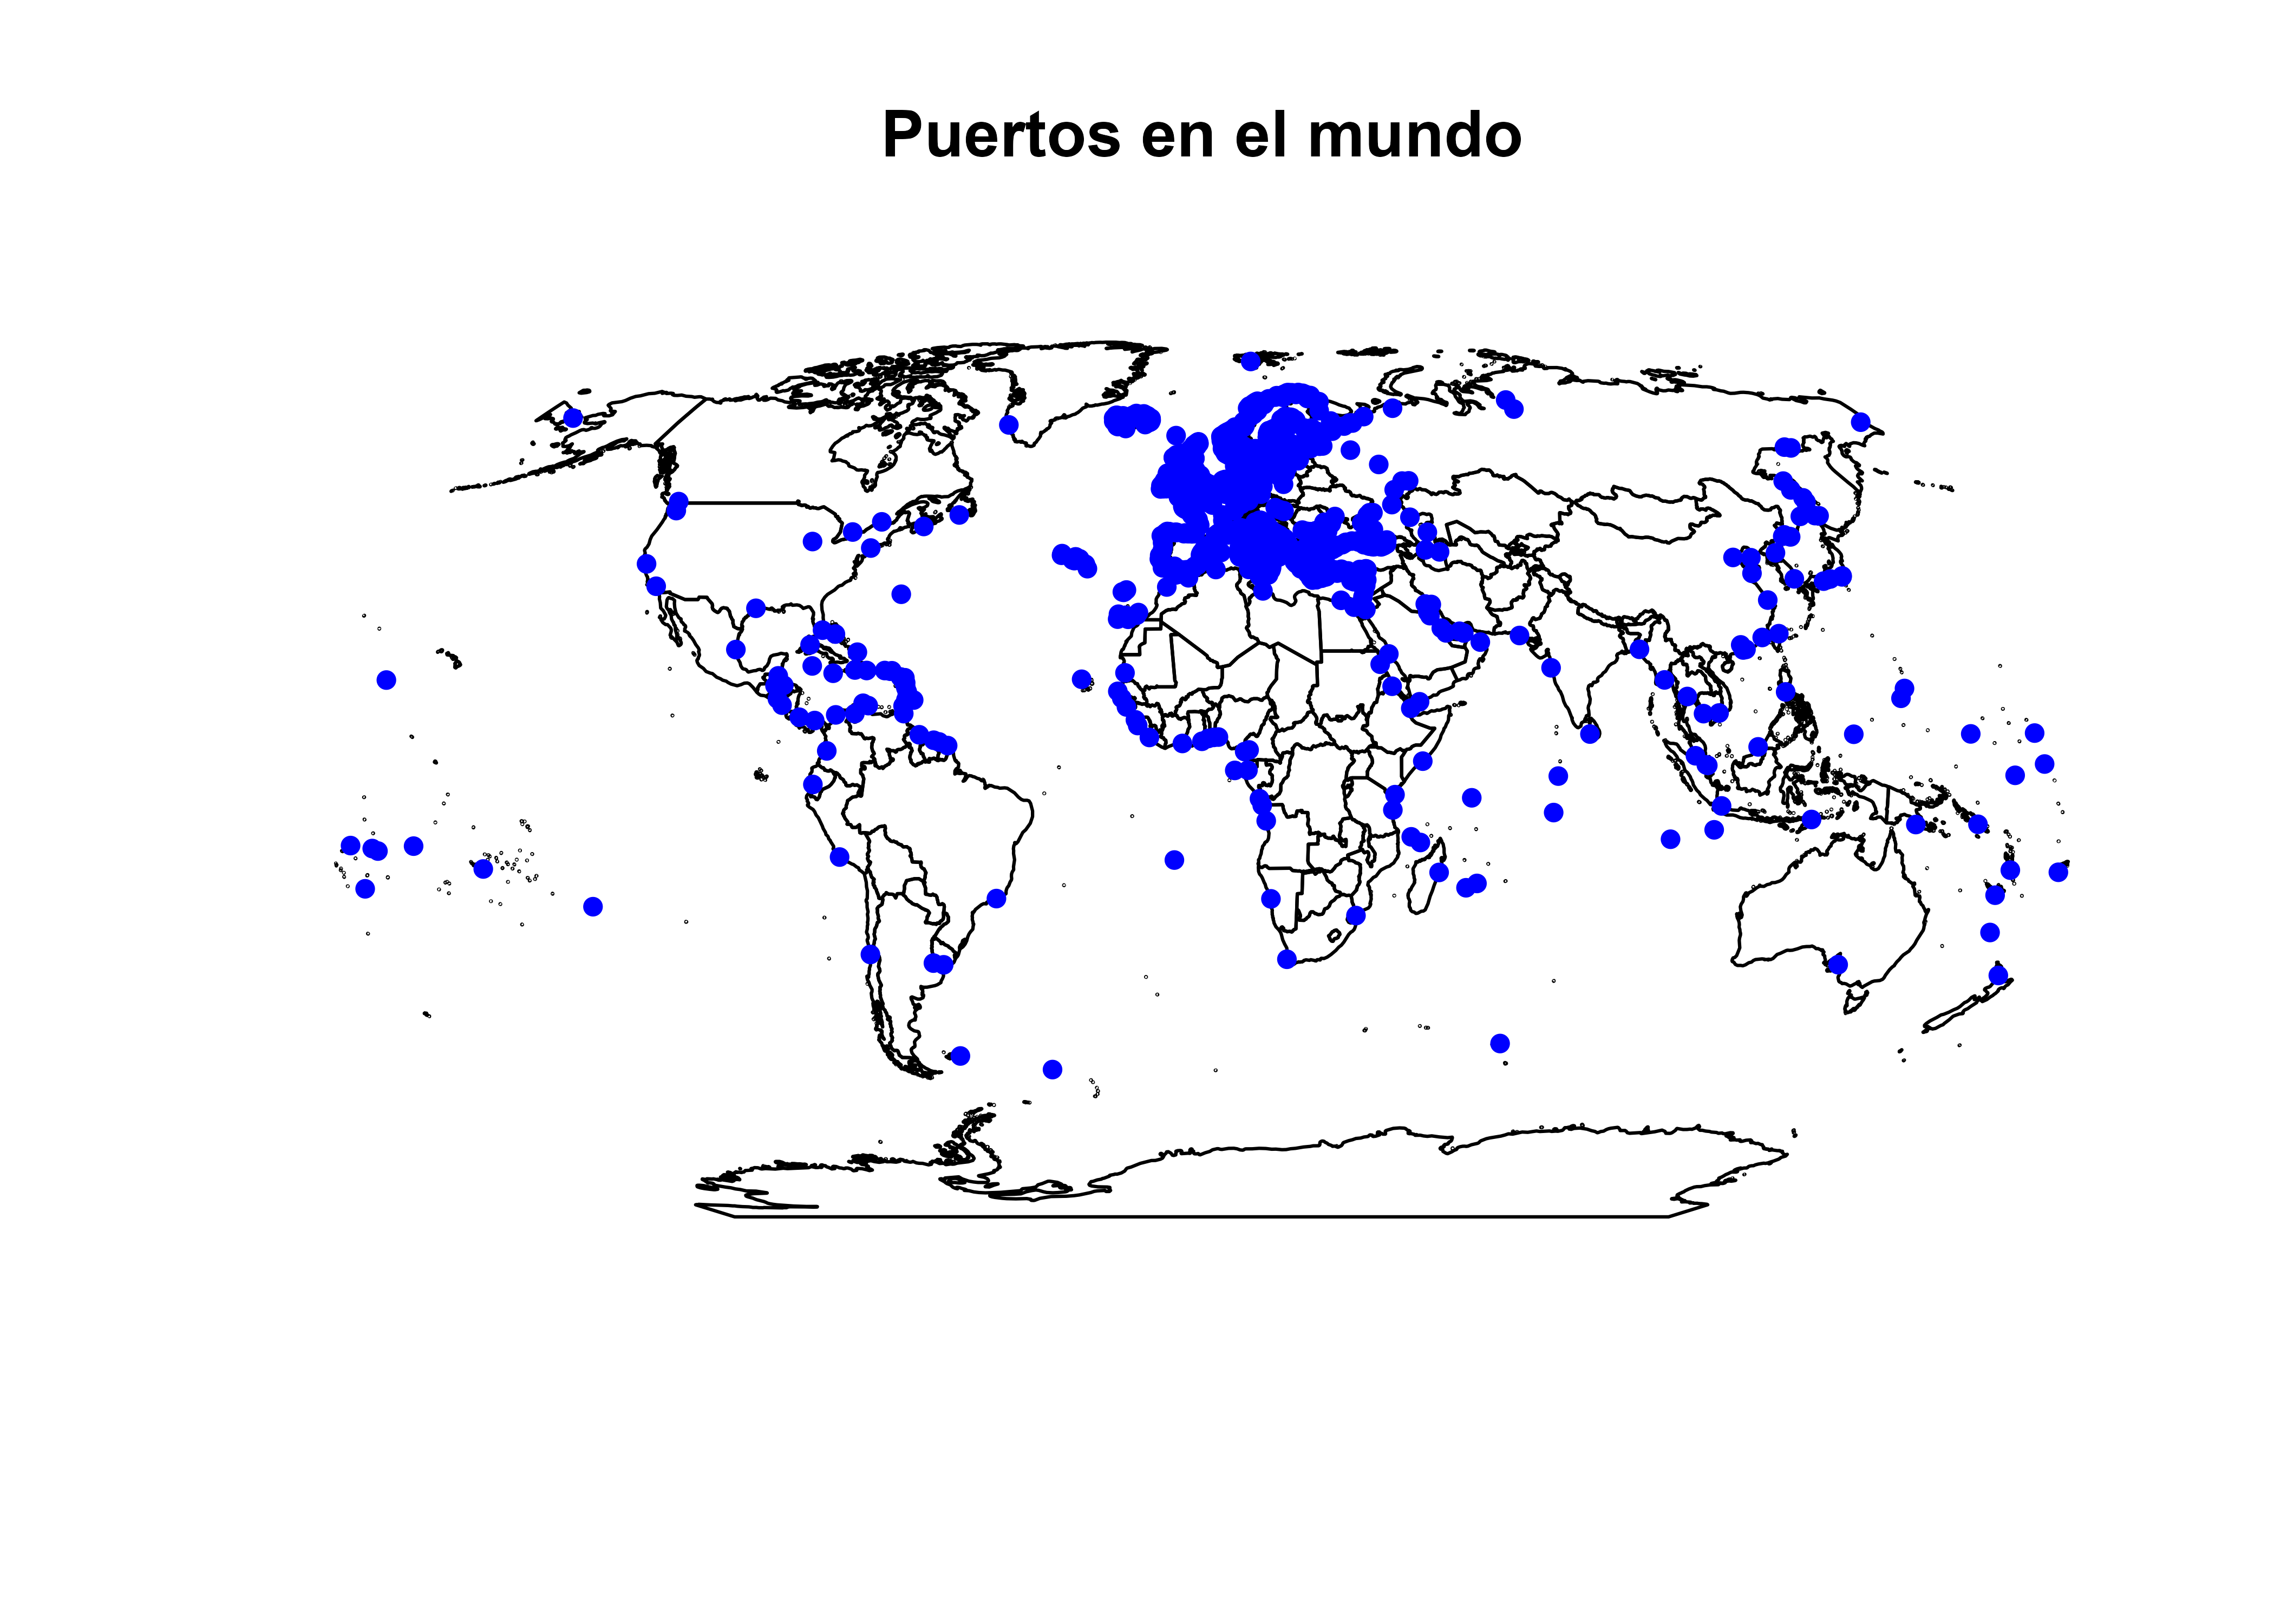
\includegraphics[width=0.6\linewidth]{_main_files/figure-latex/puertos-ok-1} 

}

\caption{Ejemplo: Puertos del mundo, CRS alineados}\label{fig:puertos-ok}
\end{figure}

Como vemos, en el primer mapa (Fig. \ref{fig:puertos-error}) los puertos se
concentran en un único punto, dado que no están referenciados en el mismo CRS.
Tras proyectarlos al mismo CRS, el mapa se representa adecuadamente (Fig.
\ref{fig:puertos-ok}).

En otros paquetes, como \texttt{sp} o \texttt{raster}, existen funciones parecidas que nos van
a permitir obtener los parámetros de un CRS y proyectar los objetos al CRS
deseado. Cuando empleemos el paquete \texttt{sp} podemos usar las funciones \texttt{CRS()} y
\texttt{spTransform()}:

\begin{Shaded}
\begin{Highlighting}[]

\FunctionTok{library}\NormalTok{(sp)}

\CommentTok{\# Convertimos sf a sp}
\NormalTok{paises\_sp }\OtherTok{\textless{}{-}} \FunctionTok{as}\NormalTok{(paises, }\StringTok{"Spatial"}\NormalTok{)}

\CommentTok{\# En sp podemos usar:}
\CommentTok{\# CRS("+proj=robin")}
\CommentTok{\#}
\CommentTok{\# O también desde sf}
\CommentTok{\# CRS(st\_crs(paises\_robin)$proj4string)}


\NormalTok{paises\_sp\_robin }\OtherTok{\textless{}{-}} \FunctionTok{spTransform}\NormalTok{(paises\_sp, }\FunctionTok{CRS}\NormalTok{(}\StringTok{"+proj=robin"}\NormalTok{))}
\FunctionTok{plot}\NormalTok{(paises\_sp\_robin)}
\end{Highlighting}
\end{Shaded}

\begin{figure}

{\centering 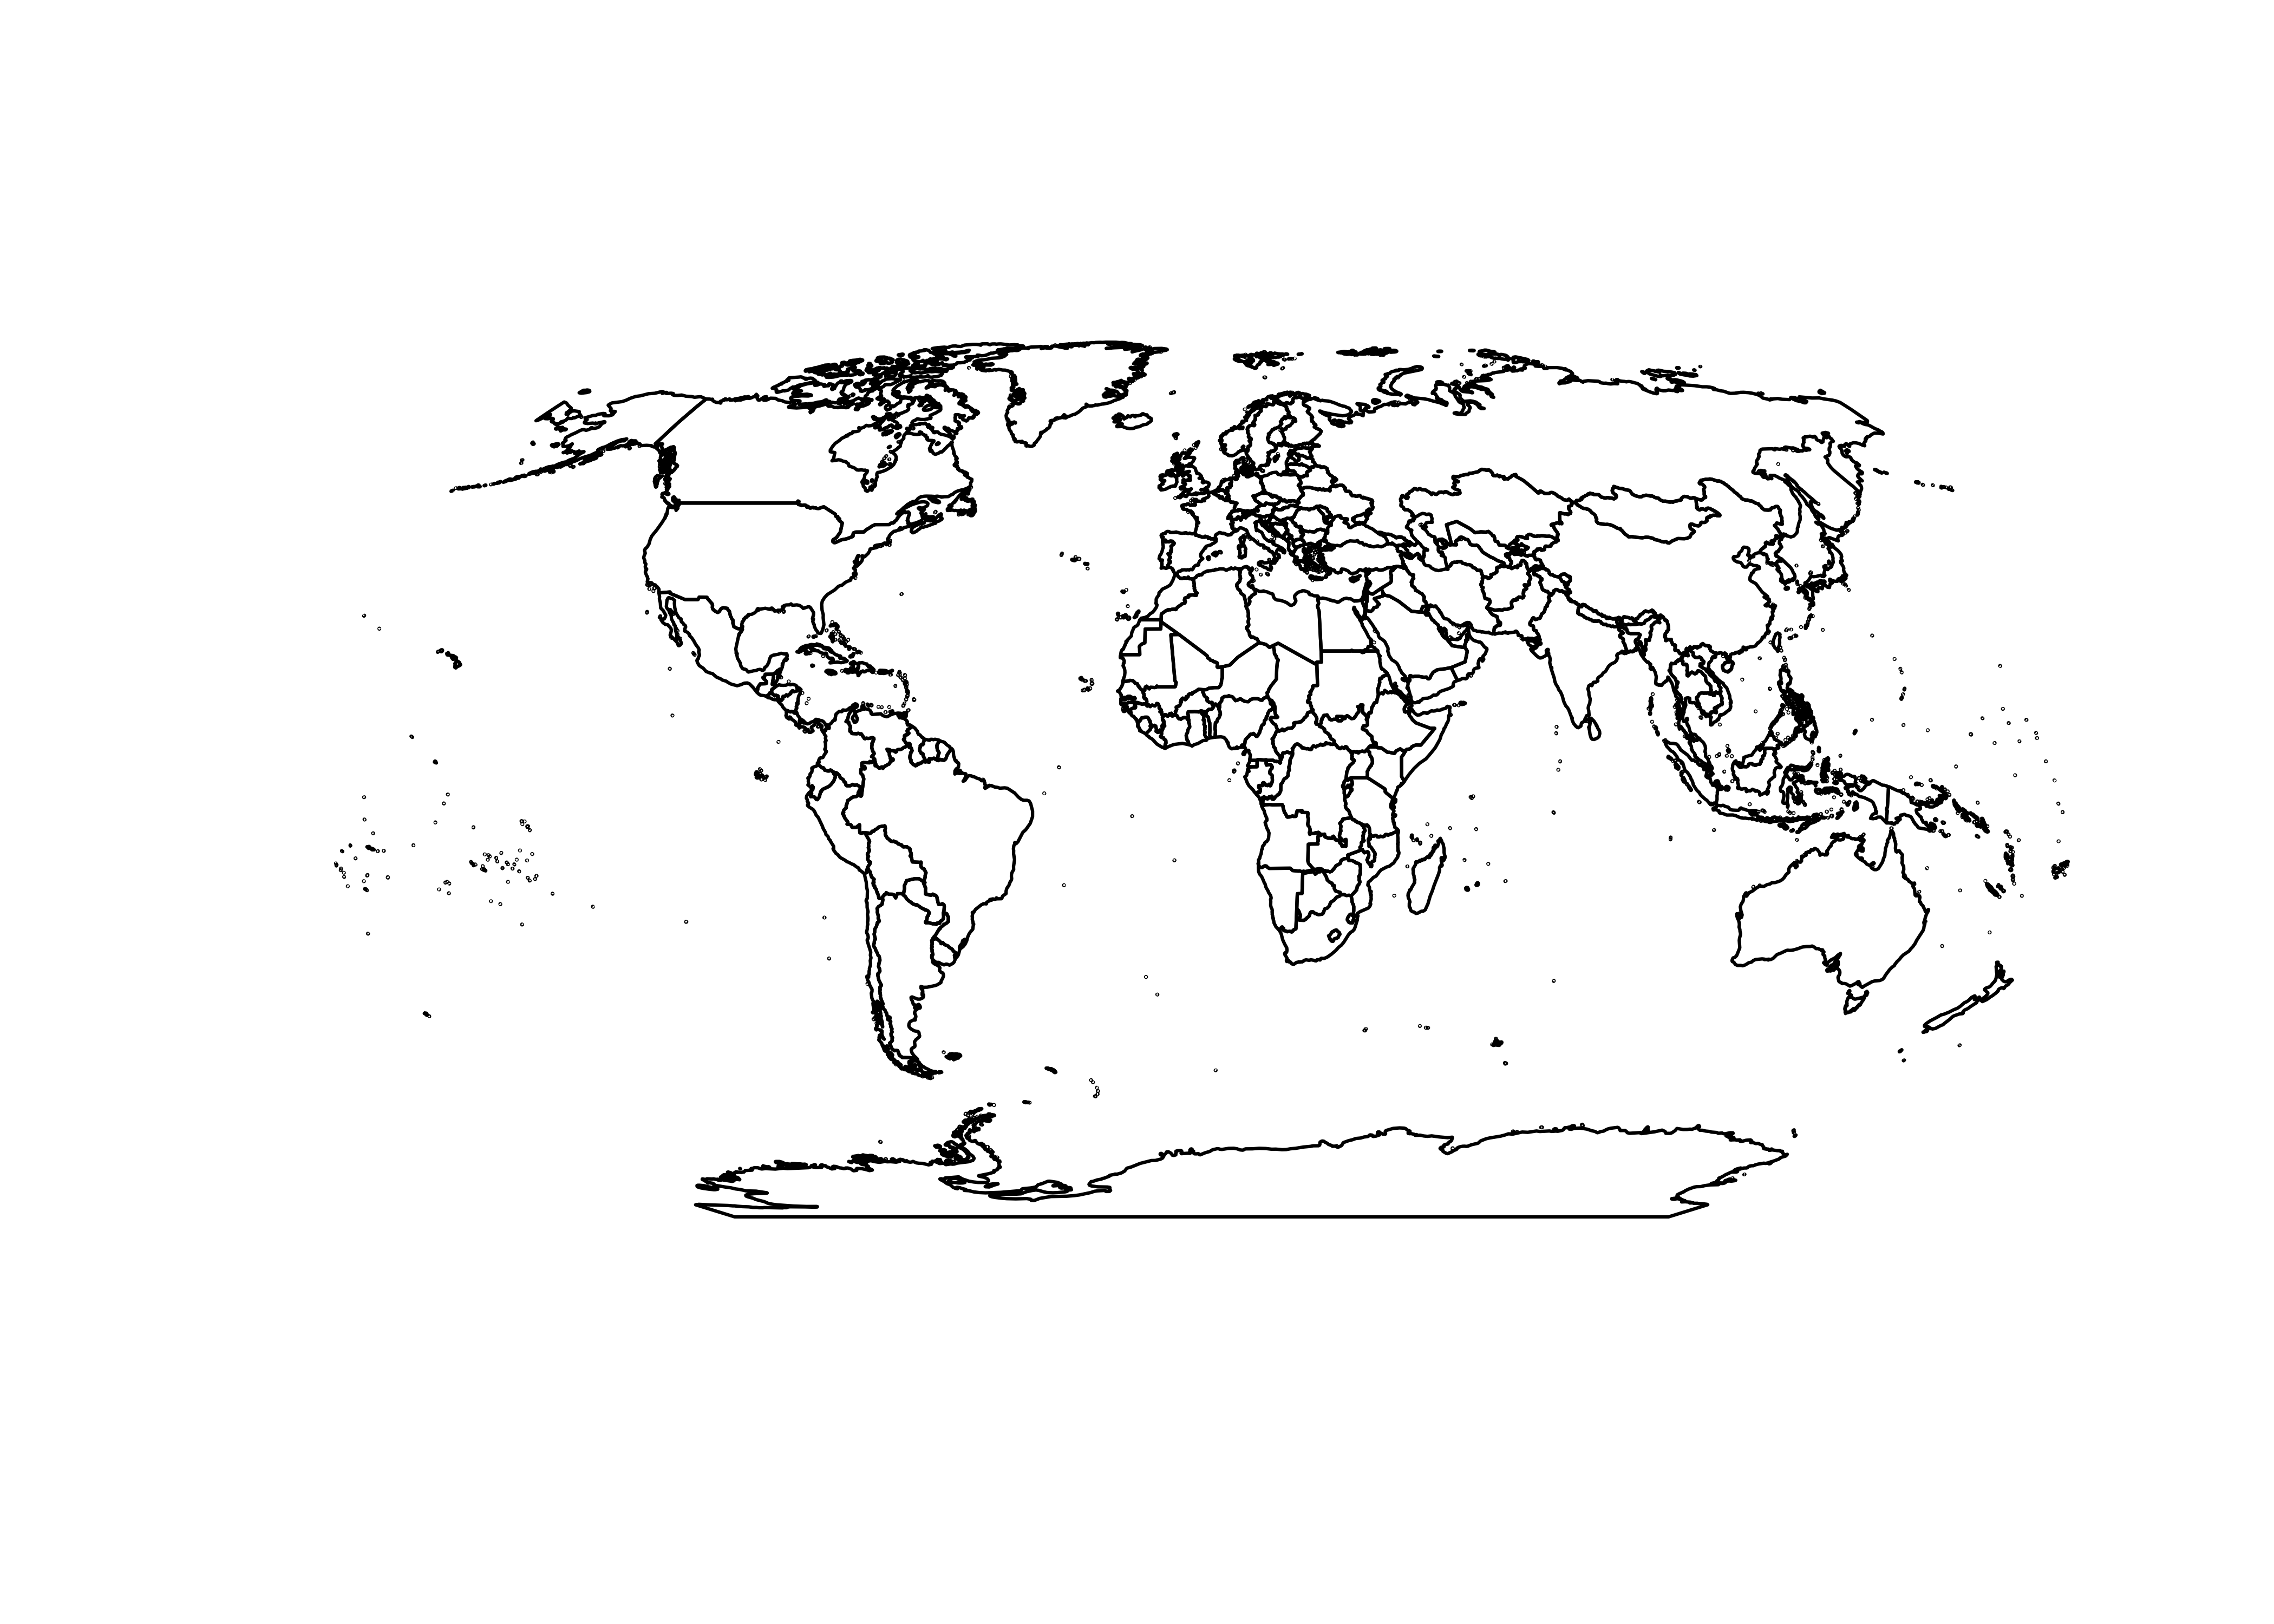
\includegraphics[width=0.6\linewidth]{_main_files/figure-latex/sp-1} 

}

\caption{Transformaciones en sp}\label{fig:sp}
\end{figure}

En el caso de un objeto \texttt{raster}, podemos usar \texttt{crs()} y \texttt{projectRaster()}:

\begin{Shaded}
\begin{Highlighting}[]
\FunctionTok{library}\NormalTok{(raster)}


\CommentTok{\# Extrae información de altitud para España}
\NormalTok{elev }\OtherTok{\textless{}{-}} \FunctionTok{raster}\NormalTok{(}\StringTok{"data/ESP\_msk\_alt.grd"}\NormalTok{)}


\CommentTok{\# Transforma}
\NormalTok{elev\_robinson }\OtherTok{\textless{}{-}} \FunctionTok{projectRaster}\NormalTok{(elev, }\AttributeTok{crs =} \FunctionTok{crs}\NormalTok{(}\StringTok{"+proj=robin"}\NormalTok{))}
\FunctionTok{plot}\NormalTok{(elev\_robinson)}
\end{Highlighting}
\end{Shaded}

\begin{figure}

{\centering 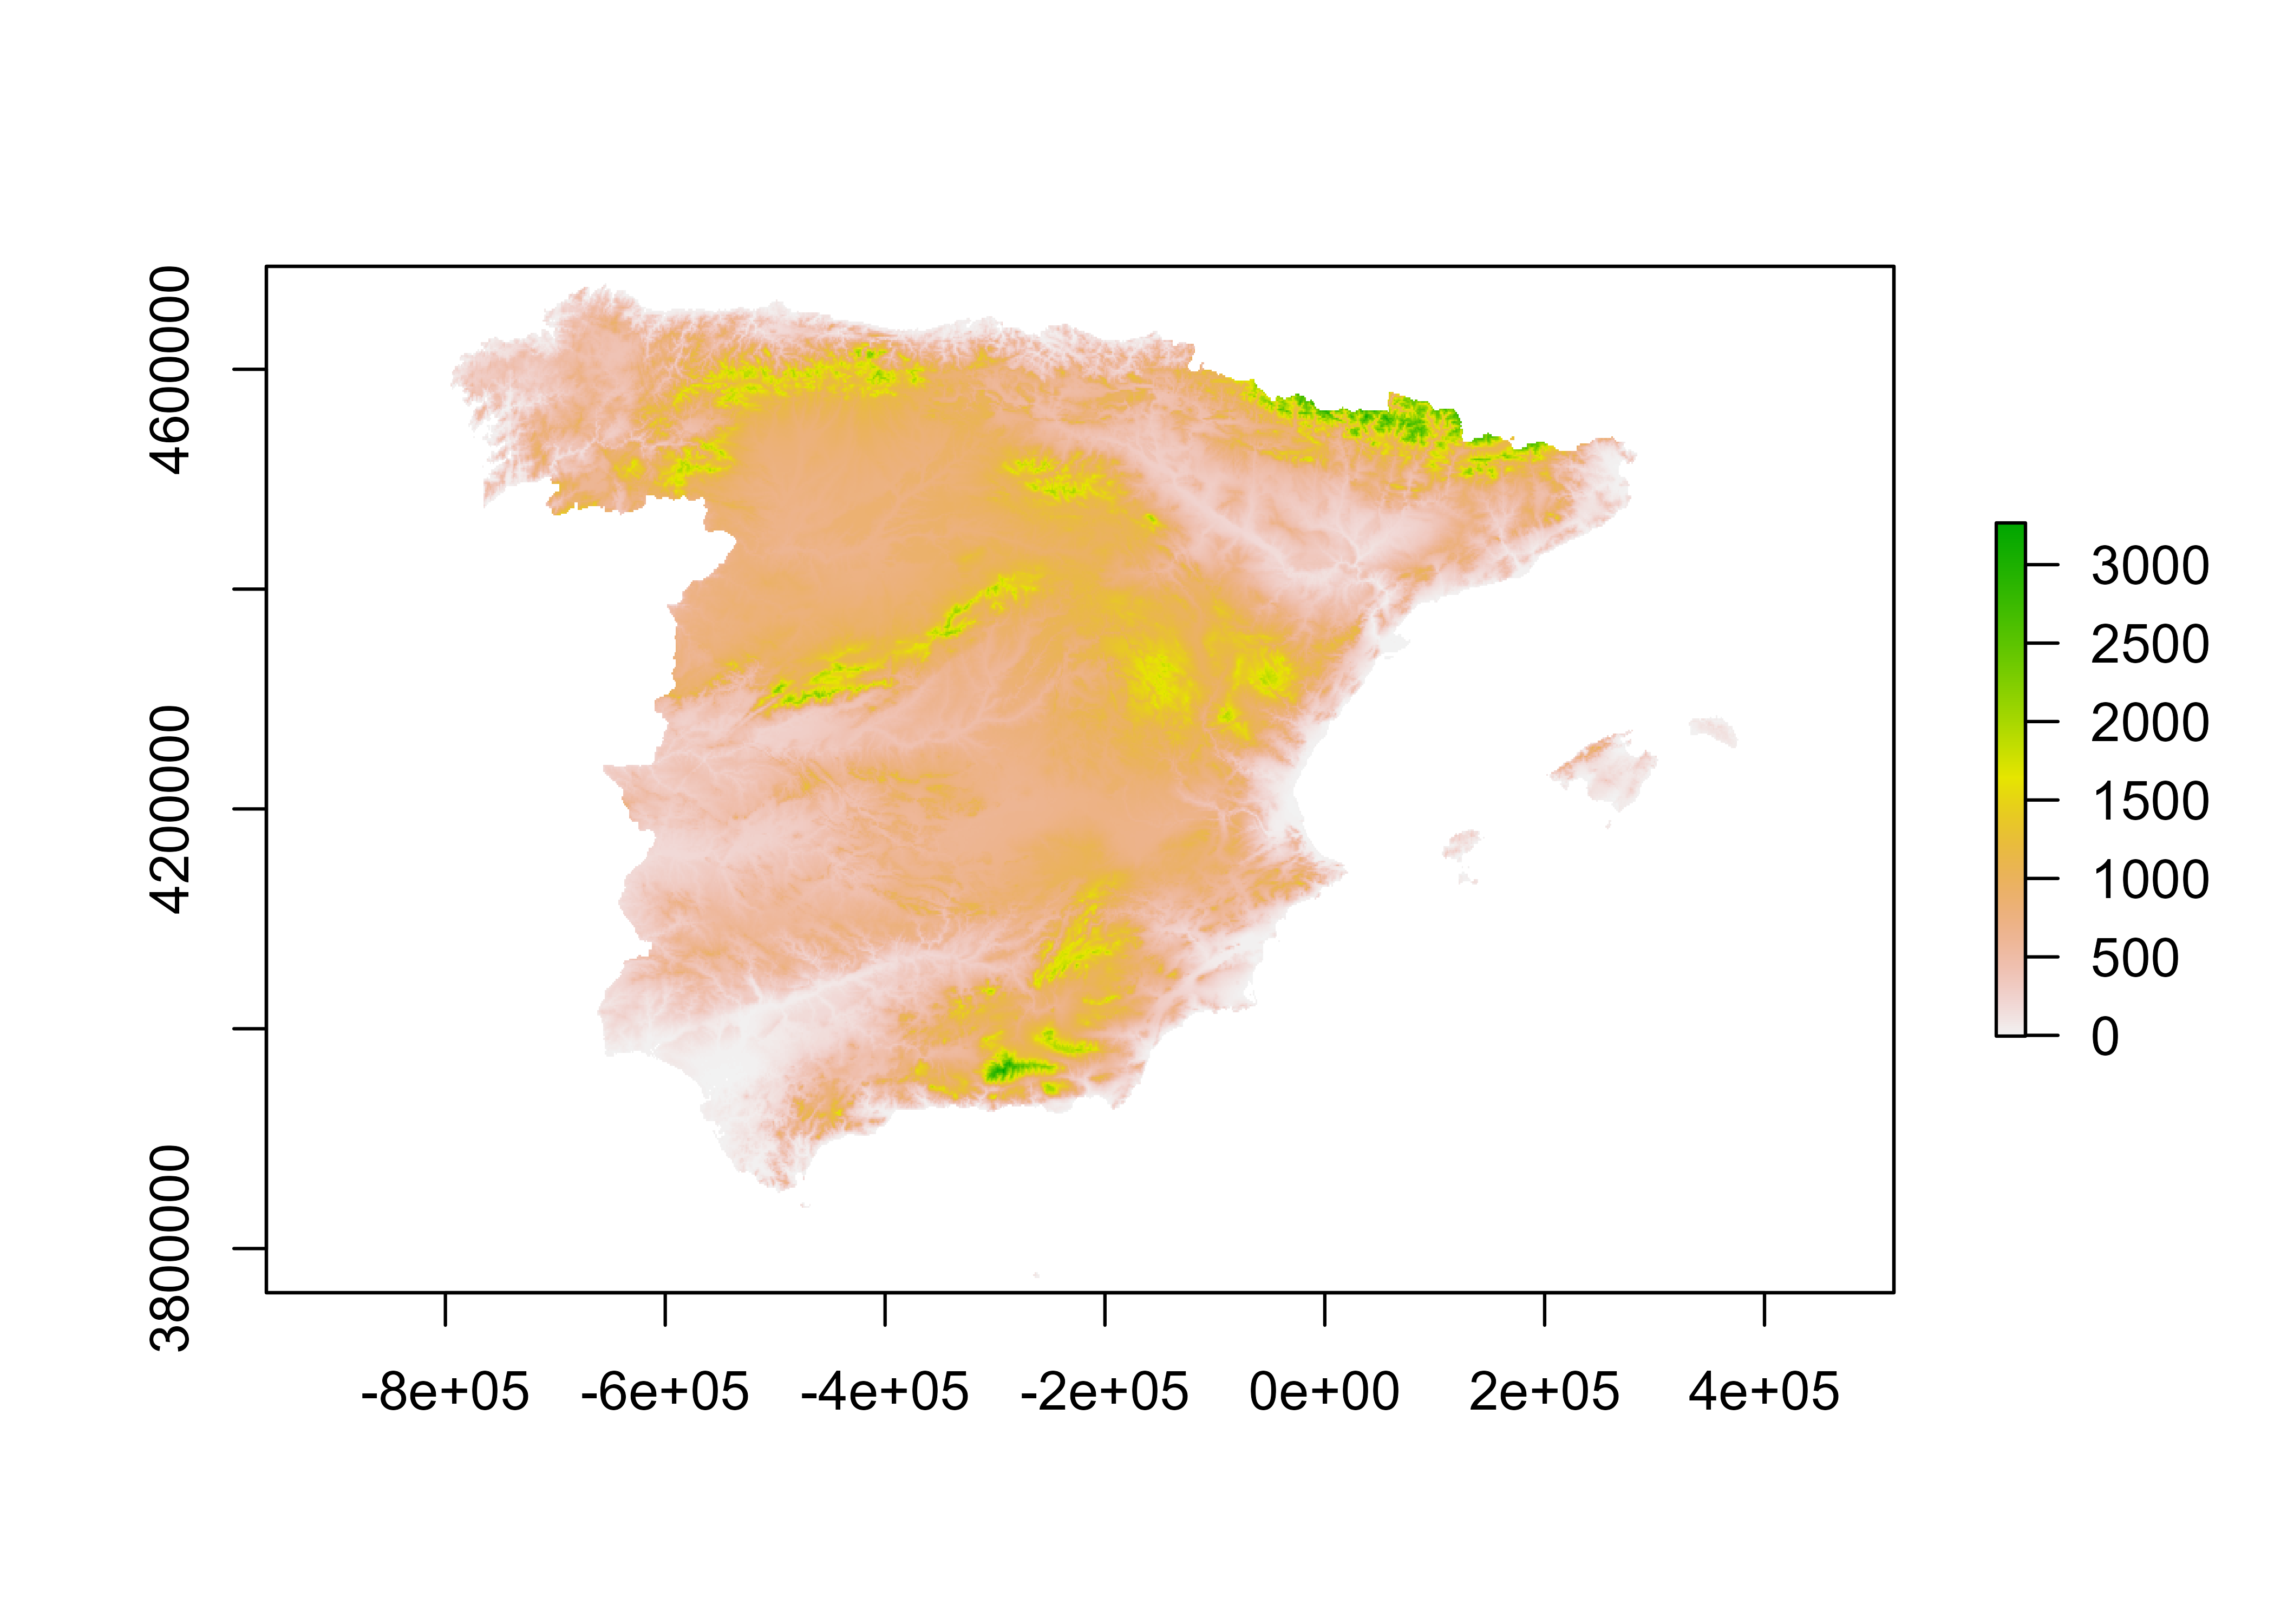
\includegraphics[width=0.6\linewidth]{_main_files/figure-latex/raster-crs-1} 

}

\caption{Transformaciones en raster}\label{fig:raster-crs}
\end{figure}

Por último, en el paquete \texttt{terra} las funciones correspondientes son \texttt{crs()} y
\texttt{project()}:

\begin{Shaded}
\begin{Highlighting}[]
\FunctionTok{library}\NormalTok{(terra)}

\CommentTok{\# Convierte de raster a terra}
\NormalTok{elev\_terra }\OtherTok{\textless{}{-}} \FunctionTok{rast}\NormalTok{(elev)}


\CommentTok{\# Transforma}
\NormalTok{elev\_terra\_robinson }\OtherTok{\textless{}{-}}\NormalTok{ terra}\SpecialCharTok{::}\FunctionTok{project}\NormalTok{(elev\_terra, terra}\SpecialCharTok{::}\FunctionTok{crs}\NormalTok{(elev\_terra))}
\FunctionTok{plot}\NormalTok{(elev\_terra\_robinson)}
\end{Highlighting}
\end{Shaded}

\begin{figure}

{\centering 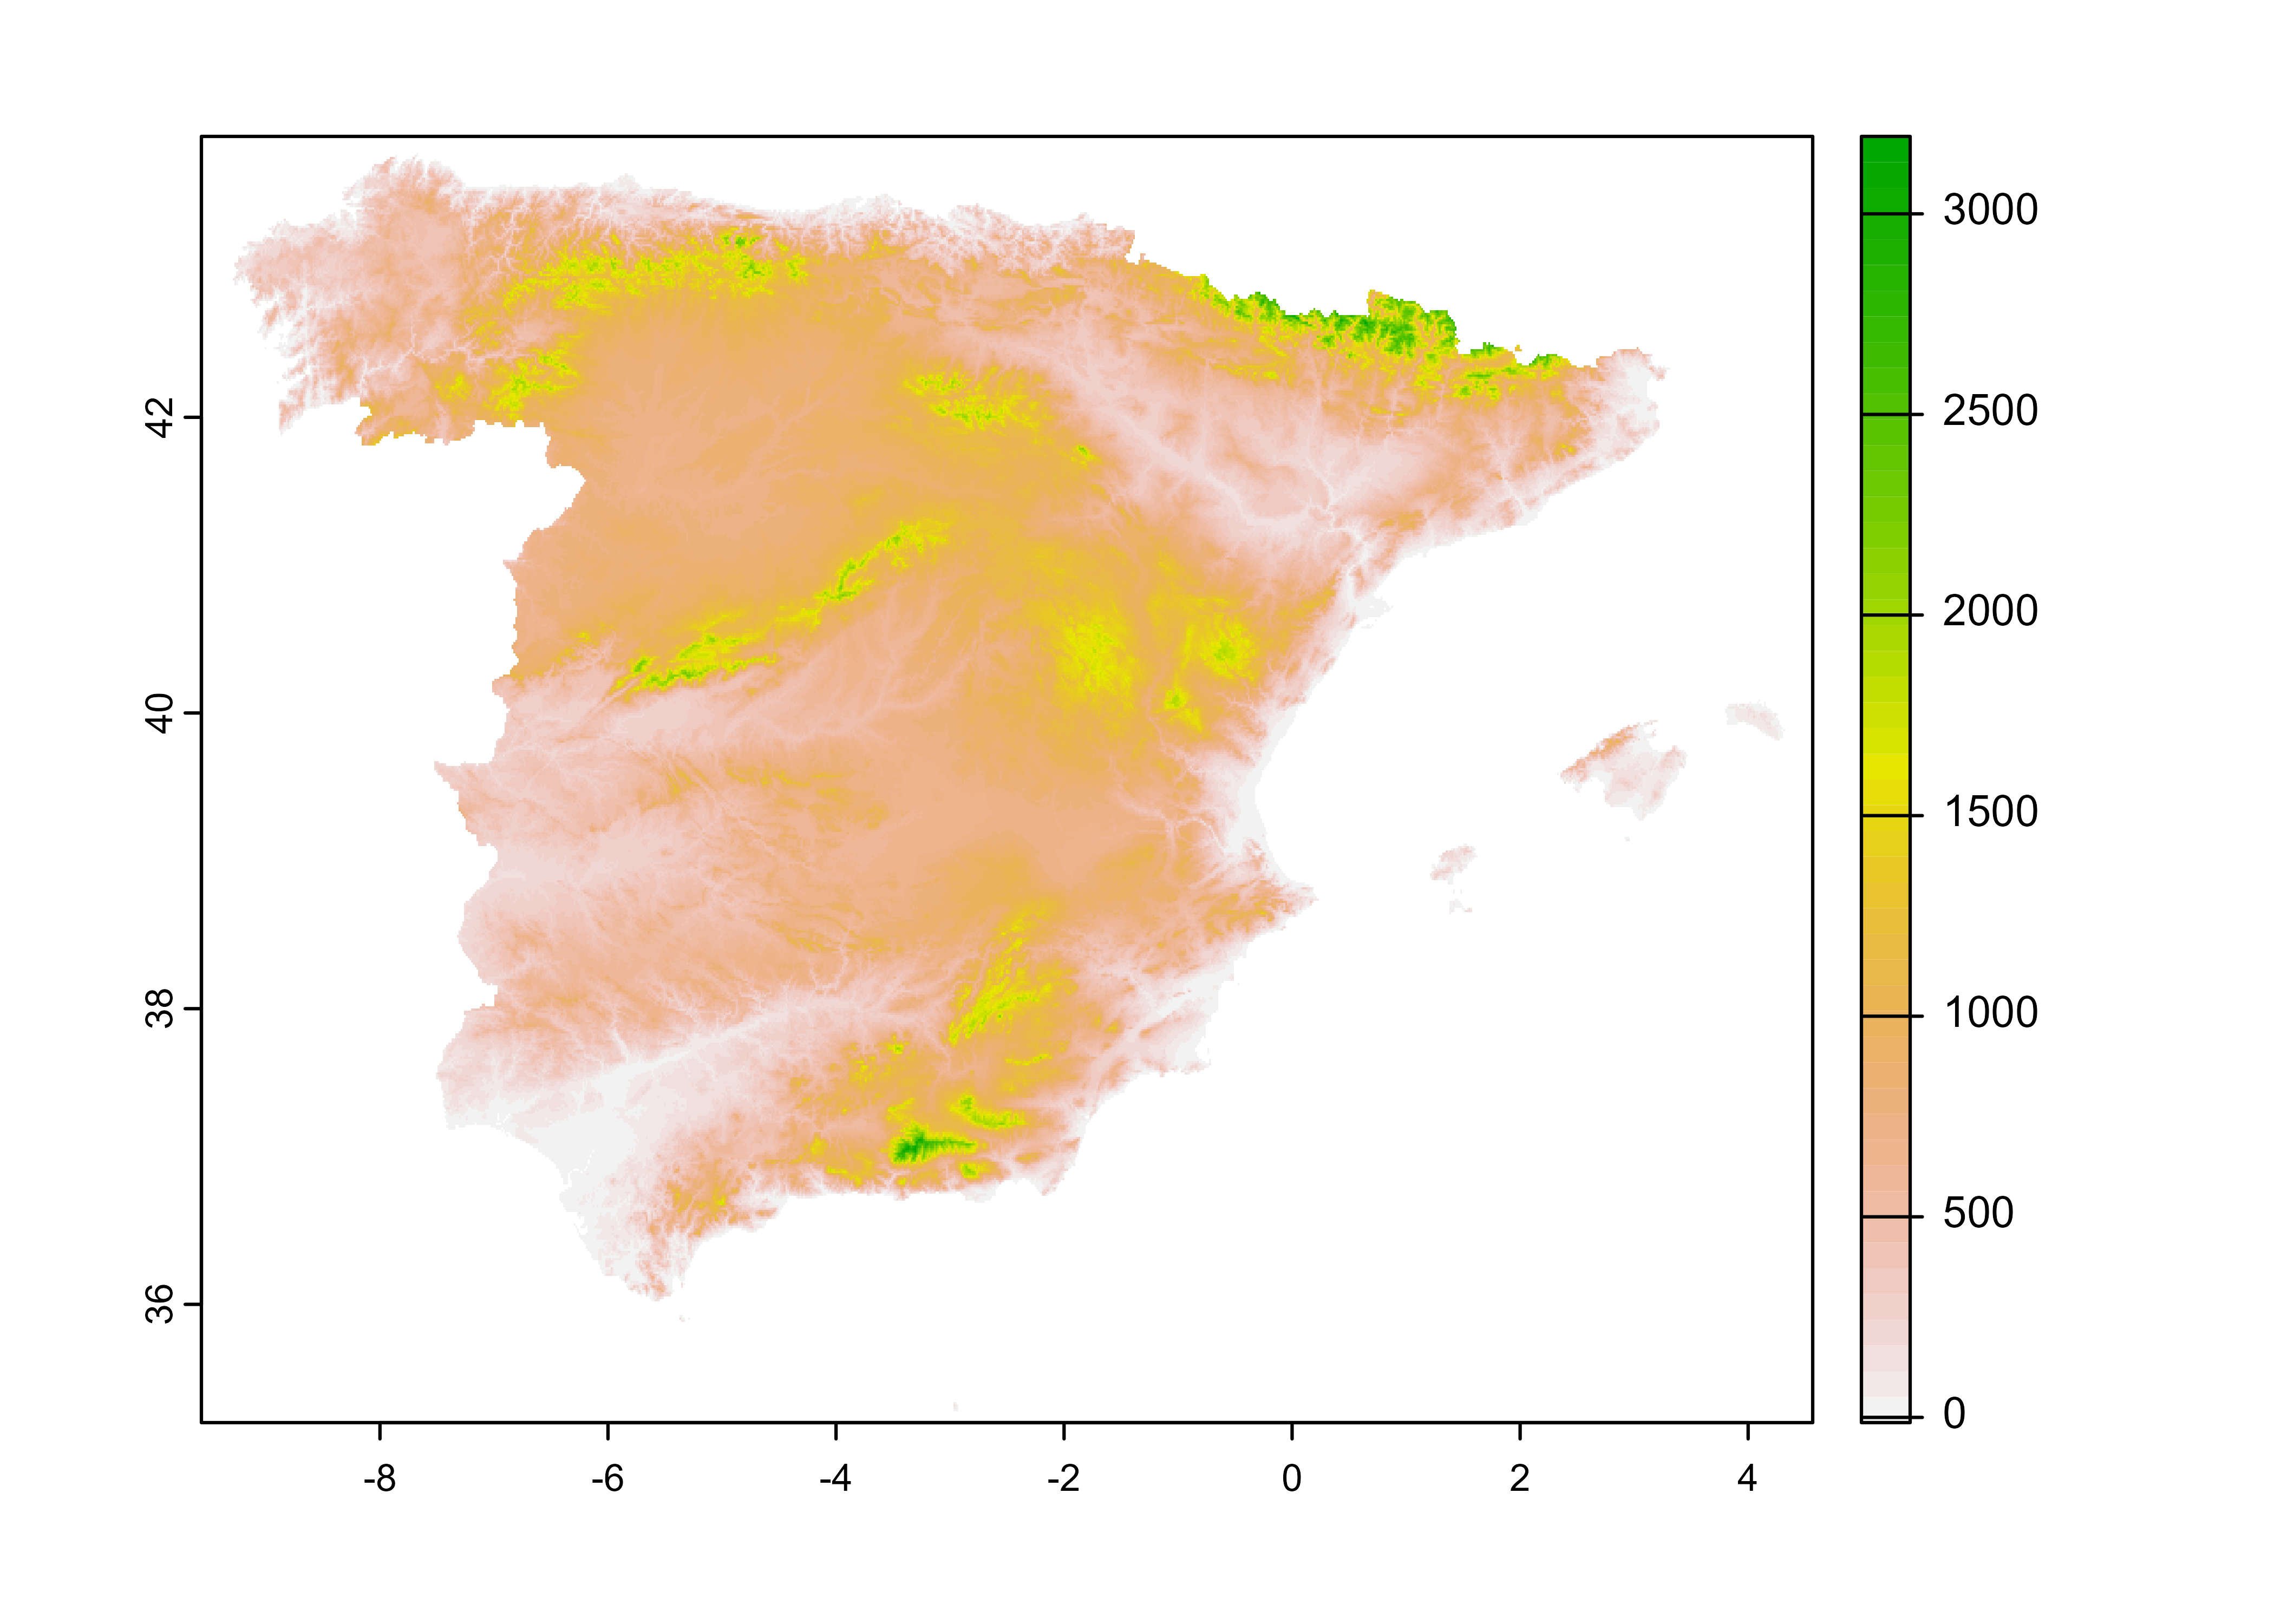
\includegraphics[width=0.6\linewidth]{_main_files/figure-latex/terra-1} 

}

\caption{Transformaciones en terra}\label{fig:terra}
\end{figure}

\hypertarget{quecrsuso}{%
\subsection{¿Qué proyección uso?}\label{quecrsuso}}

El CRS adecuado para cada análisis depende de la localización y el rango
espacial de los datos. Un CRS adecuado para representar un mapa del mundo puede
no serlo para representar datos de zonas específicas de la Tierra. Los recursos
web mencionados anteriormente permiten la búsqueda de CRS por zona geográfica, y
adicionalmente en \textbf{R} existe el paquete \texttt{crsuggest} \citep{R-crsuggest} que nos
facilita la labor, sugiriendo el CRS más adecuado para cada zona:

\begin{Shaded}
\begin{Highlighting}[]
\FunctionTok{library}\NormalTok{(crsuggest)}

\CommentTok{\# Usando raster}
\NormalTok{sugerencias }\OtherTok{\textless{}{-}} \FunctionTok{suggest\_crs}\NormalTok{(elev)}
\end{Highlighting}
\end{Shaded}

\begin{table}

\caption{\label{tab:muestra-tabla}Tabla sugerencias, detalle}
\centering
\begin{tabular}[t]{l|l|l|r|l|l}
\hline
crs\_code & crs\_name & crs\_type & crs\_gcs & crs\_units & crs\_proj4\\
\hline
2062 & Madrid 1870 (Madrid) / Spain LCC & projected & 4903 & m & +proj=lcc +lat\_1=40 +lat\_0=40 +lon\_0=0 +k\_0=0.9988085293 +x\_0=600000 +y\_0=600000 +a=6378298.3 +rf=294.73 +pm=madrid +units=m +no\_defs\\
\hline
2154 & RGF93 / Lambert-93 & projected & 4171 & m & +proj=lcc +lat\_0=46.5 +lon\_0=3 +lat\_1=49 +lat\_2=44 +x\_0=700000 +y\_0=6600000 +ellps=GRS80 +towgs84=0,0,0,0,0,0,0 +units=m +no\_defs\\
\hline
26191 & Merchich / Nord Maroc & projected & 4261 & m & +proj=lcc +lat\_1=33.3 +lat\_0=33.3 +lon\_0=-5.4 +k\_0=0.999625769 +x\_0=500000 +y\_0=300000 +ellps=clrk80ign +towgs84=31,146,47,0,0,0,0 +units=m +no\_defs\\
\hline
3944 & RGF93 / CC44 & projected & 4171 & m & +proj=lcc +lat\_0=44 +lon\_0=3 +lat\_1=43.25 +lat\_2=44.75 +x\_0=1700000 +y\_0=3200000 +ellps=GRS80 +towgs84=0,0,0,0,0,0,0 +units=m +no\_defs\\
\hline
3943 & RGF93 / CC43 & projected & 4171 & m & +proj=lcc +lat\_0=43 +lon\_0=3 +lat\_1=42.25 +lat\_2=43.75 +x\_0=1700000 +y\_0=2200000 +ellps=GRS80 +towgs84=0,0,0,0,0,0,0 +units=m +no\_defs\\
\hline
27573 & NTF (Paris) / Lambert zone III & projected & 4807 & m & +proj=lcc +lat\_1=44.1 +lat\_0=44.1 +lon\_0=0 +k\_0=0.999877499 +x\_0=600000 +y\_0=3200000 +ellps=clrk80ign +pm=paris +towgs84=-168,-60,320,0,0,0,0 +units=m +no\_defs\\
\hline
27572 & NTF (Paris) / Lambert zone II & projected & 4807 & m & +proj=lcc +lat\_1=46.8 +lat\_0=46.8 +lon\_0=0 +k\_0=0.99987742 +x\_0=600000 +y\_0=2200000 +ellps=clrk80ign +pm=paris +towgs84=-168,-60,320,0,0,0,0 +units=m +no\_defs\\
\hline
27563 & NTF (Paris) / Lambert Sud France & projected & 4807 & m & +proj=lcc +lat\_1=44.1 +lat\_0=44.1 +lon\_0=0 +k\_0=0.999877499 +x\_0=600000 +y\_0=200000 +ellps=clrk80ign +pm=paris +towgs84=-168,-60,320,0,0,0,0 +units=m +no\_defs\\
\hline
30791 & Nord Sahara 1959 / Nord Algerie & projected & 4307 & m & +proj=lcc +lat\_1=36 +lat\_0=36 +lon\_0=2.7 +k\_0=0.999625544 +x\_0=500135 +y\_0=300090 +a=6378249.145 +rf=293.465 +towgs84=-209.3622,-87.8162,404.6198,0.0046,3.4784,0.5805,-1.4547 +units=m +no\_defs\\
\hline
30493 & Voirol 1879 / Nord Algerie (ancienne) & projected & 4671 & m & +proj=lcc +lat\_1=36 +lat\_0=36 +lon\_0=2.7 +k\_0=0.999625544 +x\_0=500000 +y\_0=300000 +ellps=clrk80ign +units=m +no\_defs\\
\hline
\end{tabular}
\end{table}

\begin{Shaded}
\begin{Highlighting}[]
\CommentTok{\# Probamos sugerencia}
\NormalTok{crs\_suggest }\OtherTok{\textless{}{-}} \FunctionTok{suggest\_crs}\NormalTok{(elev, }\AttributeTok{limit =} \DecValTok{1}\NormalTok{)}

\NormalTok{elev\_suggest }\OtherTok{\textless{}{-}} \FunctionTok{projectRaster}\NormalTok{(elev, }\AttributeTok{crs =}\NormalTok{ raster}\SpecialCharTok{::}\FunctionTok{crs}\NormalTok{(crs\_suggest}\SpecialCharTok{$}\NormalTok{crs\_proj4))}

\FunctionTok{plot}\NormalTok{(elev\_suggest)}
\end{Highlighting}
\end{Shaded}

\begin{figure}

{\centering 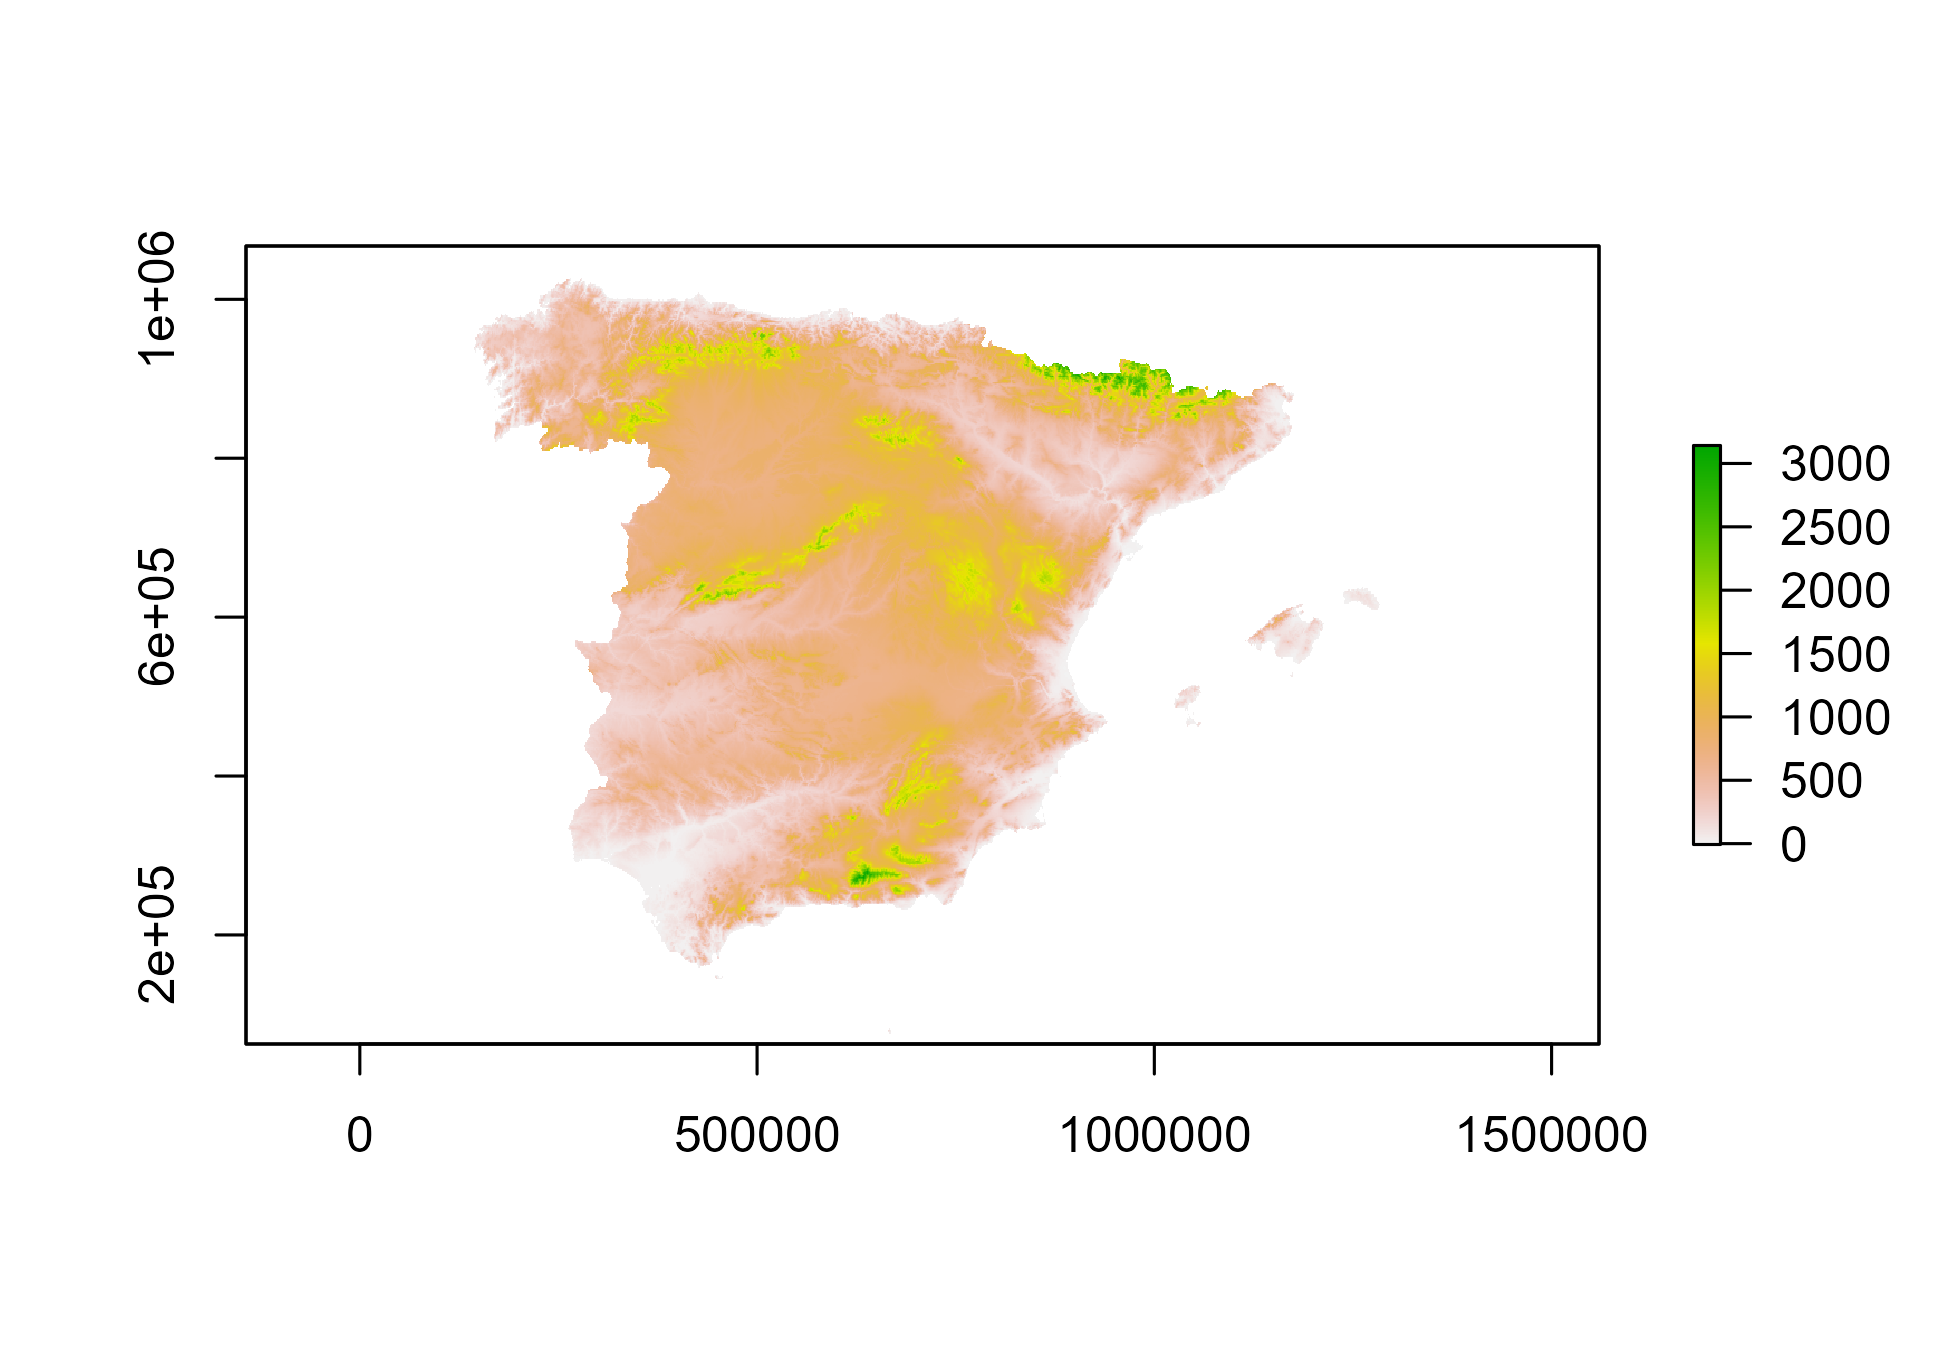
\includegraphics[width=0.6\linewidth]{_main_files/figure-latex/sugerencia-1} 

}

\caption{raster: Ejemplo de transformación usando crsuggest}\label{fig:sugerencia-1}
\end{figure}

\begin{Shaded}
\begin{Highlighting}[]

\CommentTok{\# Ejemplo con sf: China}

\NormalTok{china }\OtherTok{\textless{}{-}} \FunctionTok{gisco\_get\_countries}\NormalTok{(}\AttributeTok{country =} \StringTok{"China"}\NormalTok{)}
\NormalTok{china\_crs }\OtherTok{\textless{}{-}} \FunctionTok{suggest\_crs}\NormalTok{(china, }\AttributeTok{limit =} \DecValTok{1}\NormalTok{)}

\NormalTok{china\_crs}
\CommentTok{\#\textgreater{} \# A tibble: 1 x 6}
\CommentTok{\#\textgreater{}   crs\_code crs\_name        crs\_type crs\_gcs crs\_units crs\_proj4                 }
\CommentTok{\#\textgreater{}   \textless{}chr\textgreater{}    \textless{}chr\textgreater{}           \textless{}chr\textgreater{}      \textless{}dbl\textgreater{} \textless{}chr\textgreater{}     \textless{}chr\textgreater{}                     }
\CommentTok{\#\textgreater{} 1 4584     New Beijing / \textasciitilde{} project\textasciitilde{}    4555 m         +proj=tmerc +lat\_0=0 +lon\textasciitilde{}}


\NormalTok{china\_suggest }\OtherTok{\textless{}{-}} \FunctionTok{st\_transform}\NormalTok{(}
\NormalTok{  china,}
  \FunctionTok{st\_crs}\NormalTok{(}\FunctionTok{as.integer}\NormalTok{(china\_crs}\SpecialCharTok{$}\NormalTok{crs\_code))}
\NormalTok{)}


\FunctionTok{plot}\NormalTok{(}\FunctionTok{st\_geometry}\NormalTok{(china\_suggest), }\AttributeTok{axes =} \ConstantTok{TRUE}\NormalTok{)}
\end{Highlighting}
\end{Shaded}

\begin{figure}

{\centering 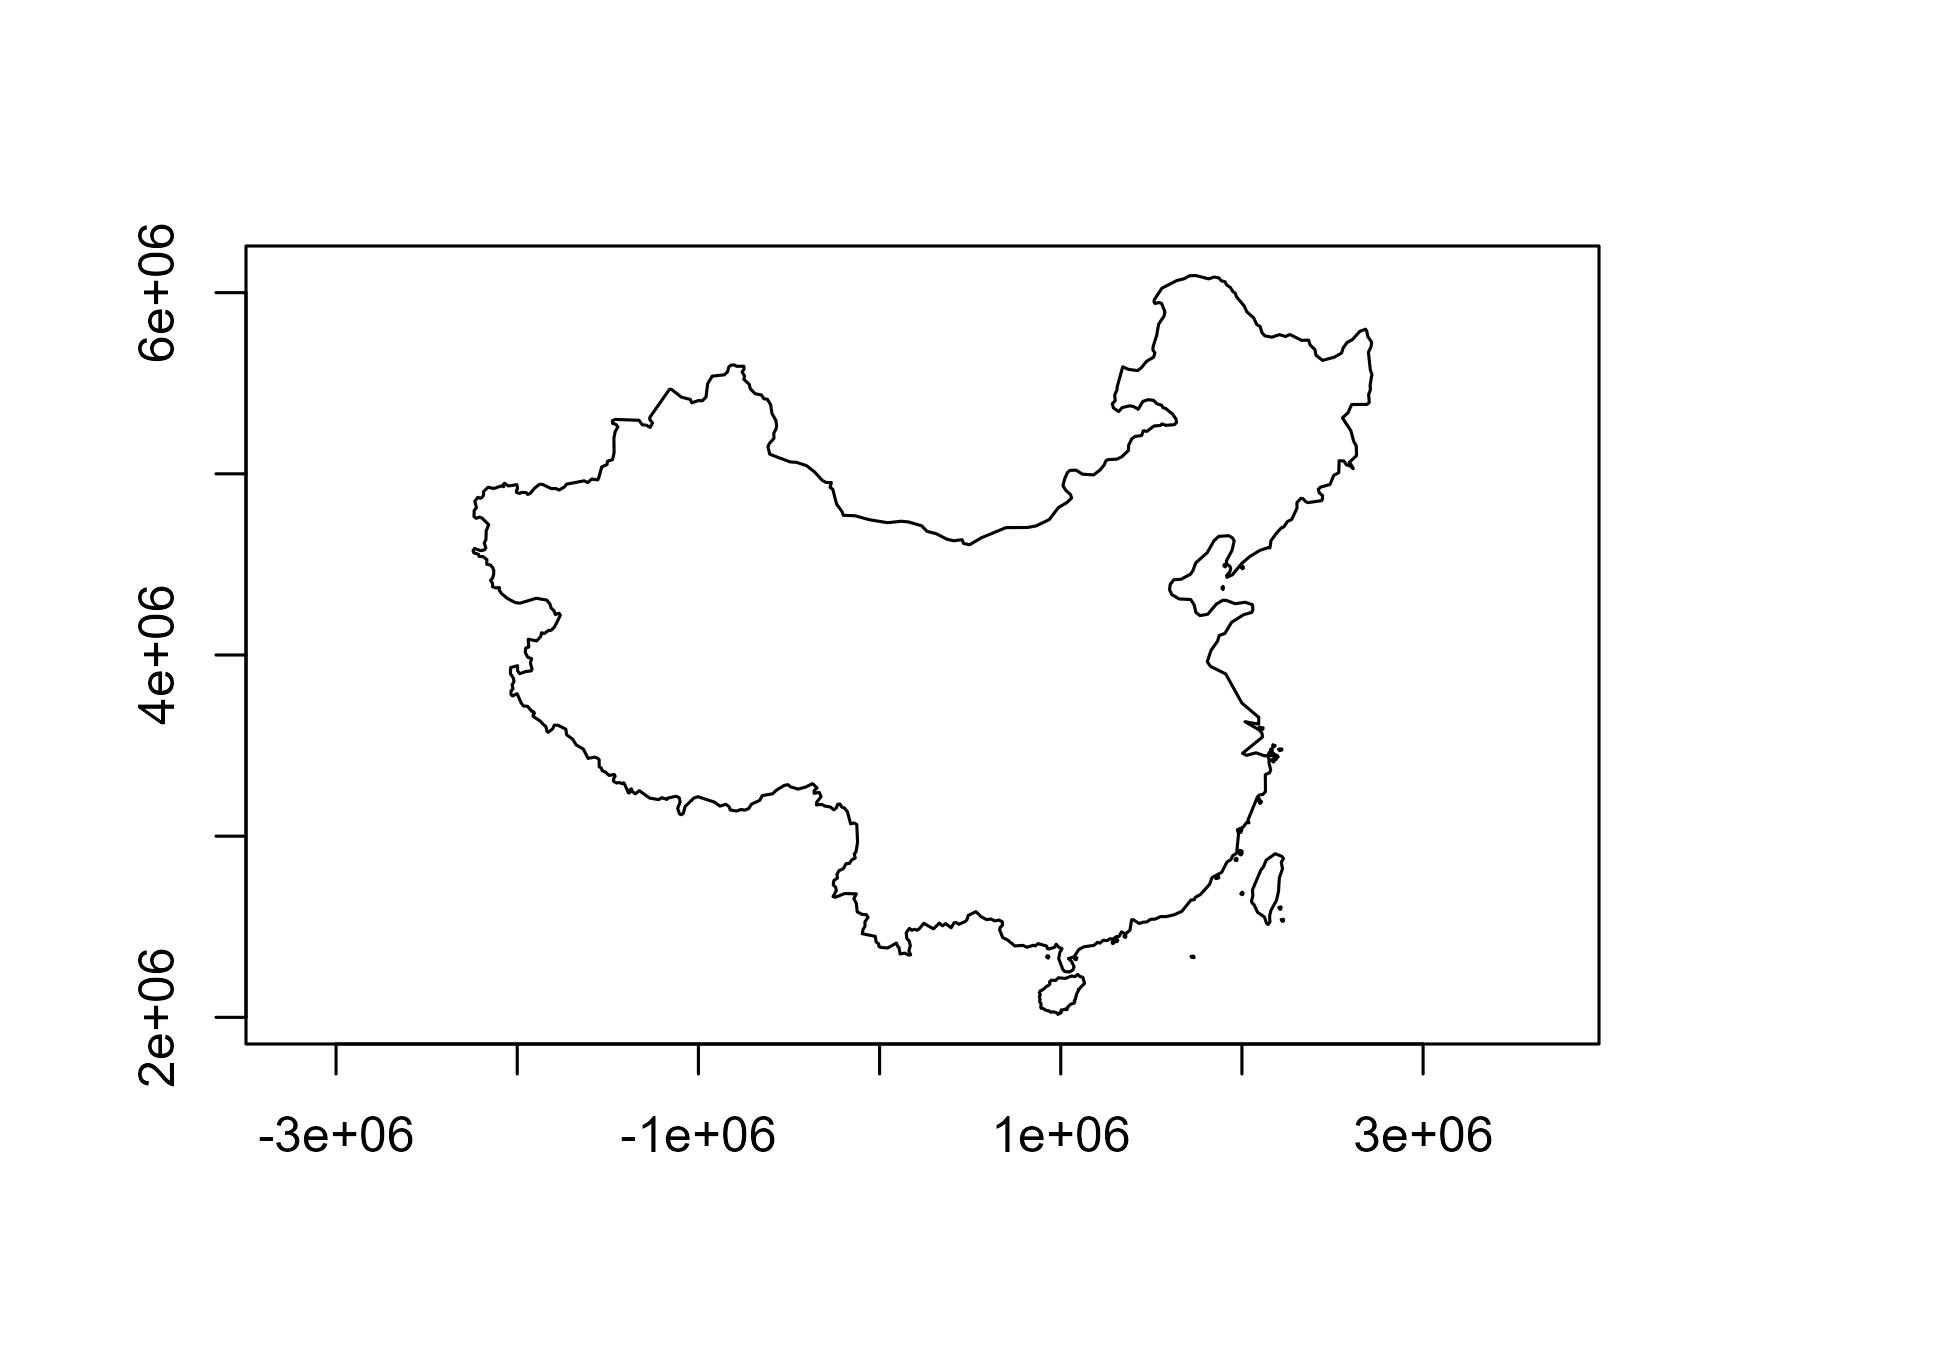
\includegraphics[width=0.6\linewidth]{_main_files/figure-latex/sugerencia-2} 

}

\caption{sf: Ejemplo de transformación usando crsuggest}\label{fig:sugerencia-2}
\end{figure}

\hypertarget{dep-esp}{%
\chapter{Estadística espacial}\label{dep-esp}}

La estadística espacial se basa en la suposición de que las unidades
georreferenciadas cercanas están relacionadas (son \textbf{dependientes}) de
alguna manera \citep{getis_1999}, y por ello, trata de reconocer y aprovechar ésta
ubicación espacial a la hora de diseñar, recopilar, gestionar,
analizar y mostrar las observaciones (\citet{montero_et_al_2011}).

Los métodos estadísticos espaciales que se utilizan actualmente,
y sobre los que continúan las investigaciones, incluyen el estudio de la
asociación espacial, el análisis de patrones, la escala y la zonificación,
la geoestadística, la clasificación, el muestreo espacial
y la econometría espacial. Estos métodos se aplican a una gran variedad
de disciplinas científicas. Por ejemplo, \citet{montero_et_al_2011}
destacan los siguientes. Los orígenes de la vida humana vinculan los estudios
de la evolución de las galaxias, la estructura de las
células biológicas y los patrones de asentamiento arqueológicos. Los ecologistas
estudian las interacciones entre plantas y animales. Silvicultores y
agricultores necesitan investigar las variaciones que se producen en el terreno
para sus experimentos. La estimación de las precipitaciones y de las reservas de
oro y petróleo es de vital importancia económica. Estos son, entre otros, buenos
ejemplos de la importancia del espacio (espacio-tiempo en su caso) en el mundo
de la Ciencia.

Sin embargo, el estudio de la \textbf{variabilidad espacial}, y sobre todo
espacio-temporal, es una disciplina relativamente nueva en el marco de la
Estadística, lo que explica la escasez de instrumentos de estadística espacial
30 años atrás. En los últimos 10 años ha habido una creciente toma de conciencia
de esta necesidad, habiéndose realizado un gran esfuerzo por buscar herramientas
adecuadas y útiles a tales efectos. Y todo ello porque utilizar modelos
espaciales o espacio-temporales para caracterizar y explotar la dependencia
espacial (o espacio-temporal) de un conjunto de observaciones tiene importantes
ventajas (\citet{montero_et_al_2011}):

\begin{enumerate}
\def\labelenumi{\arabic{enumi}.}
\item
  Modelos más generales, ya que, en la mayoría de los casos, los modelos
  clásicos que no tienen en consideración la dimensión espacial o la
  interacción de las dimensiones espacial y temporal son un caso particular de
  un modelo espacial o espacio-temporal.
\item
  Estimaciones más eficientes: de la tendencia, de los efectos de las
  variables explicativas, de promedios regionales,\ldots{}
\item
  Mejora de las predicciones: más eficientes, con propiedades de extrapolación
  más estables,\ldots{}
\item
  La variación espacial no explicada en la estructura de la media debe ser
  absorbida por la estructura del error, por lo que un modelo que incorpore la
  dependencia espacial puede decirse que está protegido frente a una mala
  especificación de este tipo. Esto, en muchos casos, tiene como resultado una
  simplificación en la especificación de la tendencia; en general, los modelos
  con dependencia espacial suelen tener una descripción más parsimoniosa (en
  ocasiones con muchos menos parámetros) que los clásicos modelos de
  superficie de tendencia.
\end{enumerate}

\hypertarget{antes-de-continuar-dependencia-espacial.}{%
\section{Antes de continuar\ldots{} dependencia espacial.}\label{antes-de-continuar-dependencia-espacial.}}

Frecuentemente los datos tienen una componente espacial y/o temporal asociada a
ellos y es de esperar que datos cercanos en el espacio o en el tiempo sean más
semejantes que aquellos que están más alejados; en cuyo caso \textbf{no} deben ser
modelados como estadísticamente independiente, sino que habrá que tomar en
cuenta esa dependencia espacial o espacio-temporal.

De forma natural y de acuerdo a la Ley Tobler (1973) surge la idea de que los
datos cercanos en el espacio o en el tiempo serán más similares y estarán más
correlacionados entres sí que aquellos que están más lejanos.
Por ejemplo, la influencia de un terremoto, su efecto disminuye
con distancia del epicentro. Además, esta correlación disminuye al aumentar
la separación entre ellos, por lo que se puede
pensar en la presencia de una dependencia espacial o espacio-temporal.

Si los datos no exhiben dependencia espacial no tiene sentido aplicar las
herramientas de estadística espacial. ¿Y cómo se pueden reconocer un proceso
con dependencia espacial? La clave esta en que los procesos con dependencia
espacial exiben un patrón en el espacio, mientras que los que son independientes
son totalmente aleatorios.

La Fig. \ref{fig:points-depiid} muestra uno campo aleatorio simulado que presentan una
estructura de dependencia espacial (panel izquierdo) frente a unos datos
totalmente aleatorios (panel derecho), en ambos casos distribuidos de forma
irregular en el espacio. En la imagen de dependencia espacial se observa como
los puntos rojos (que representan valores más altos de la variable simuladas)
se concentran en la misma zona, al igual que los puntos azules (que representan valores más bajos)
que se distribujen en otra zona y juntos.

\begin{figure}

{\centering 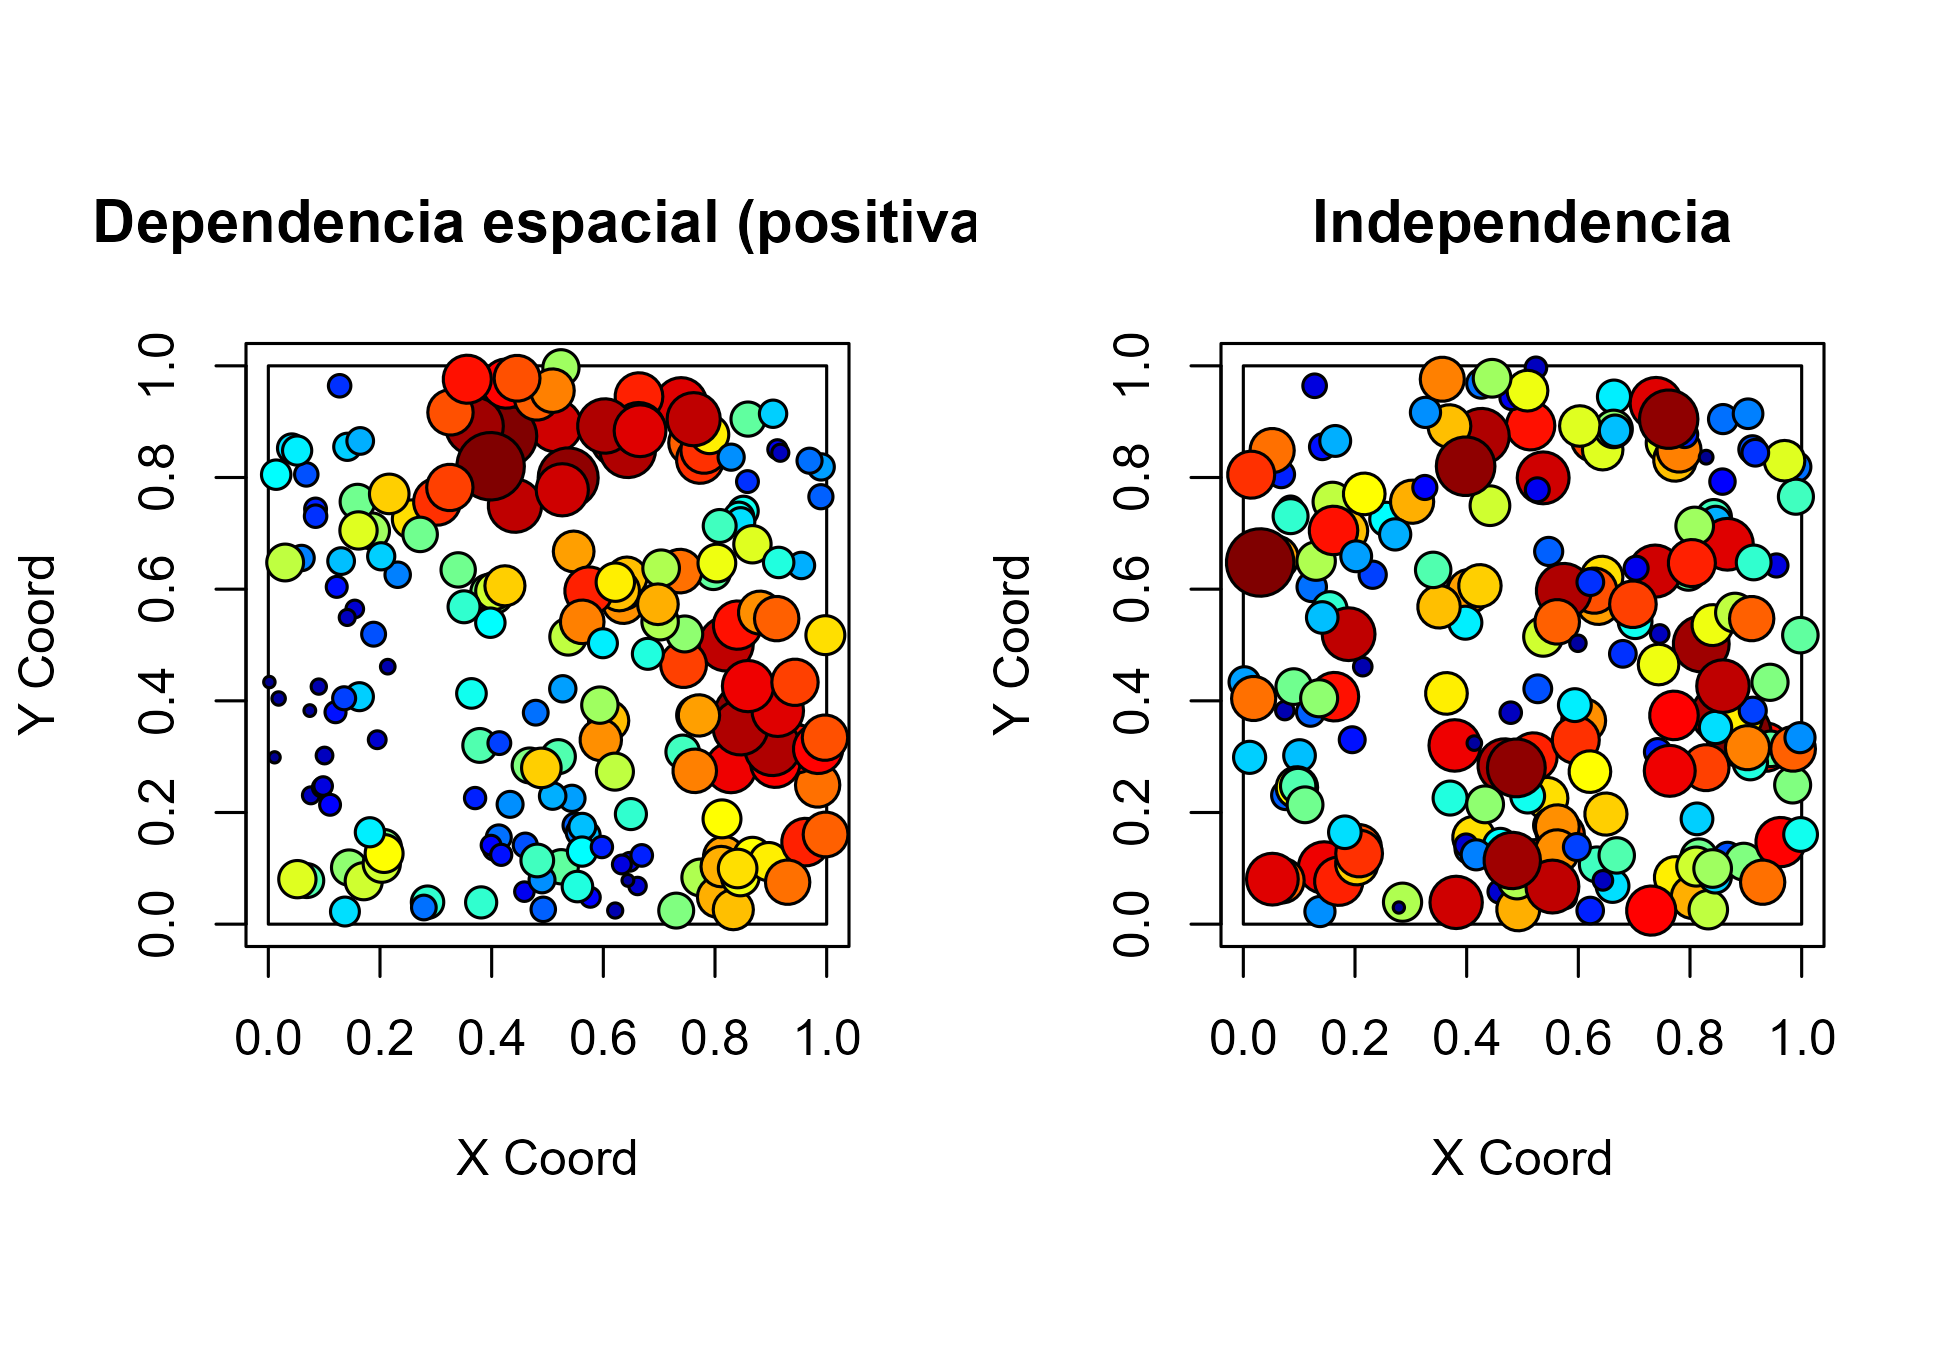
\includegraphics[width=0.6\linewidth]{_main_files/figure-latex/points-depiid-1} 

}

\caption{Puntos: Simulación patrón de independencia espacial (derecha) frente a dependencia espacial (izquierda)}\label{fig:points-depiid}
\end{figure}

La Fig. \ref{fig:lattice-dep-iid}, al igual que la Fig.
\ref{fig:points-depiid} presenta unos datos simulados donde que muestran una
estructura de dependencia espacial (panel izquierdo) frente a unos datos
totalmente aleatorios (panel derecho), pero en este caso estos datos se
distribuyen de forma ordenada en el espacio a través de una rejilla regular.
La interpretación es análoga a la de la Fig. \ref{fig:points-depiid},
solo que en este caso los campos aleatorios simulados se representan en una
rejilla.

\begin{figure}

{\centering 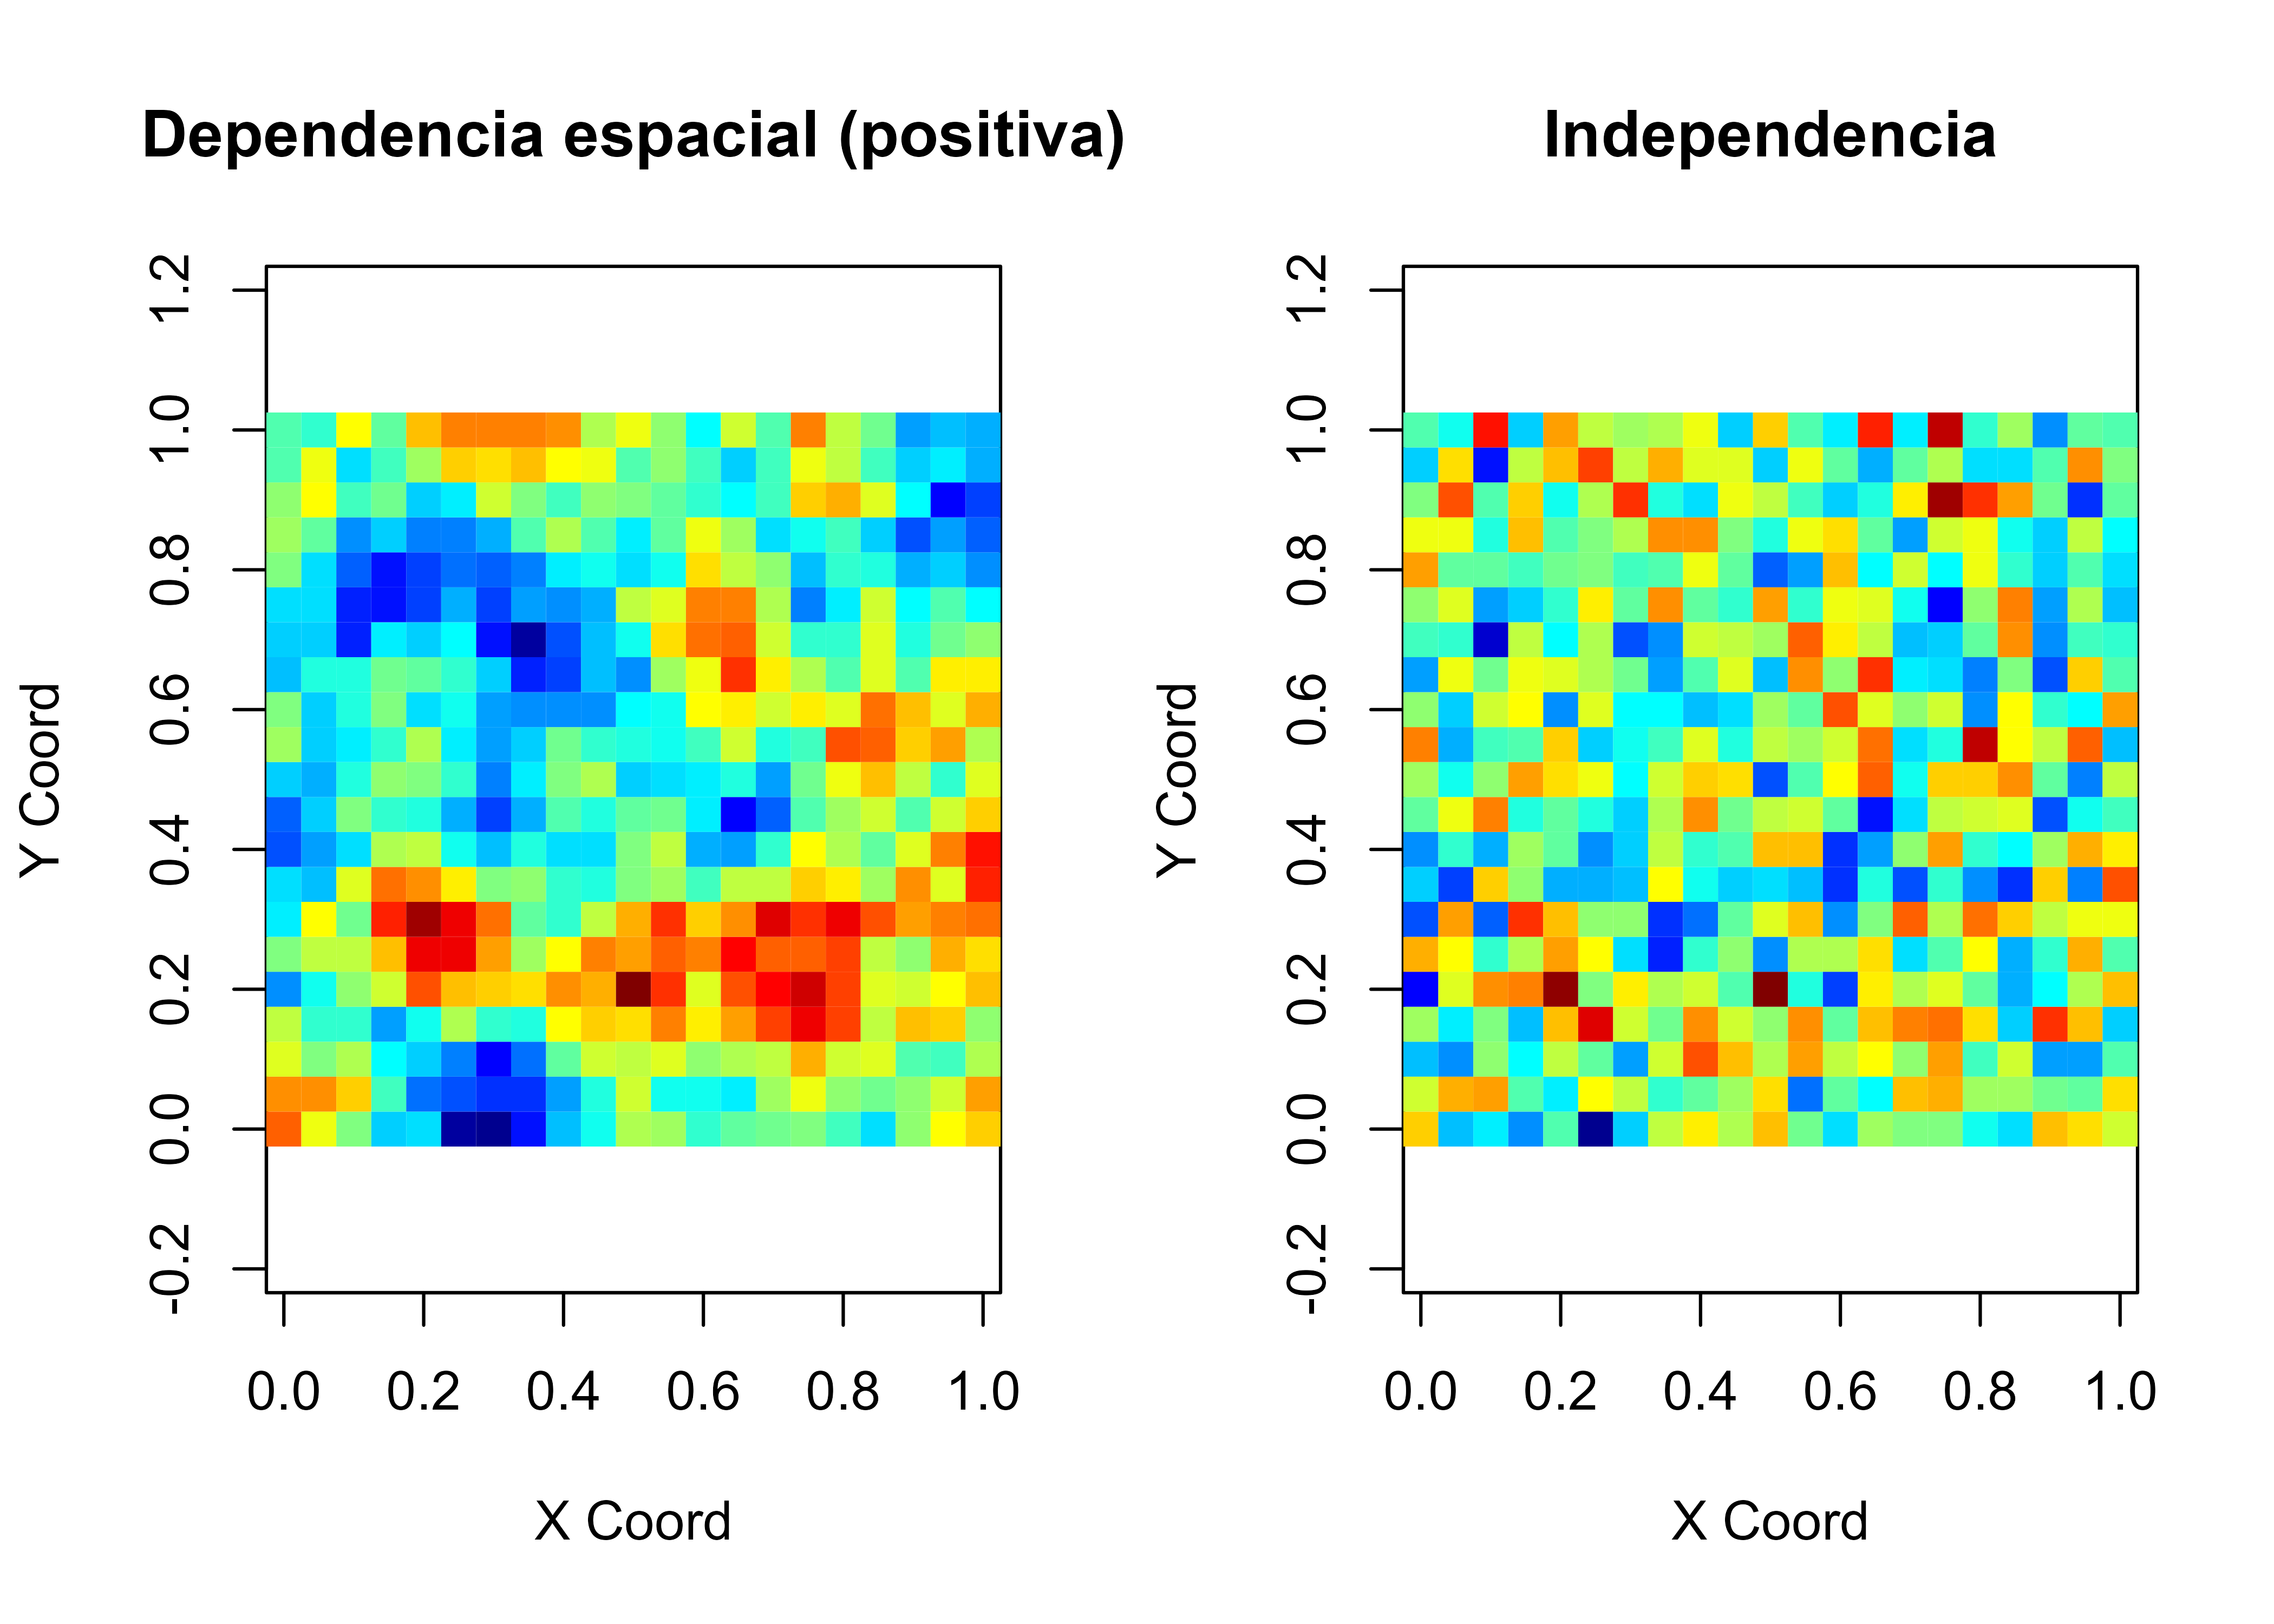
\includegraphics[width=0.6\linewidth]{_main_files/figure-latex/lattice-dep-iid-1} 

}

\caption{Rejilla: Simulación patrón de independencia espacial (derecha) frente a dependencia espacial (izquierda)}\label{fig:lattice-dep-iid}
\end{figure}

\hypertarget{datos-espaciales}{%
\section{Datos espaciales}\label{datos-espaciales}}

Los \textbf{datos espaciales}, también conocidos como datos \textbf{geoespaciales}, son
aquellos datos relacionados o que contienen información de una localización o
área geográfica de la superficie de la Tierra.

La forma más intuitiva de representar los datos espaciales es a través de un
mapa.

\begin{Shaded}
\begin{Highlighting}[]
\CommentTok{\# Mapa de porcentaje de mujeres en Castilla{-}La Mancha}

\FunctionTok{library}\NormalTok{(mapSpain)}

\CommentTok{\# Datos de población}
\NormalTok{pob }\OtherTok{\textless{}{-}}\NormalTok{ mapSpain}\SpecialCharTok{::}\NormalTok{pobmun19}


\CommentTok{\# Datos en forma de tabla, sin información en formato espacial}
\CommentTok{\# head(pob)}

\CommentTok{\# Porcentaje}
\NormalTok{pob}\SpecialCharTok{$}\NormalTok{porc\_mujeres }\OtherTok{\textless{}{-}}\NormalTok{ pob}\SpecialCharTok{$}\NormalTok{women }\SpecialCharTok{/}\NormalTok{ pob}\SpecialCharTok{$}\NormalTok{pob19 }\SpecialCharTok{*} \DecValTok{100}

\CommentTok{\# Datos espaciales}
\NormalTok{geo }\OtherTok{\textless{}{-}} \FunctionTok{esp\_get\_munic}\NormalTok{(}\AttributeTok{region =} \StringTok{"Castilla{-}La Mancha"}\NormalTok{)}

\CommentTok{\# Estos datos tienen una columna (geometry) con coordenadas.}
\CommentTok{\# head(geo)}

\CommentTok{\# Une ambos datos}
\NormalTok{geo\_pob }\OtherTok{\textless{}{-}} \FunctionTok{merge}\NormalTok{(geo,}
\NormalTok{  pob,}
  \AttributeTok{by =} \FunctionTok{c}\NormalTok{(}\StringTok{"cpro"}\NormalTok{, }\StringTok{"cmun"}\NormalTok{),}
  \AttributeTok{all.x =} \ConstantTok{TRUE}
\NormalTok{)}

\CommentTok{\# Mapa básico}
\FunctionTok{plot}\NormalTok{(geo\_pob[}\StringTok{"porc\_mujeres"}\NormalTok{],}
  \CommentTok{\# Cambiamos titulo}
  \AttributeTok{main =} \StringTok{"Castilla{-}La Mancha: \% mujeres (2019)"}\NormalTok{,}

  \CommentTok{\# Cambiamos la paleta de colores para hacerlo mas atractivo}
  \CommentTok{\# border = NA,}
  \AttributeTok{pal =} \FunctionTok{hcl.colors}\NormalTok{(}\DecValTok{12}\NormalTok{, }\StringTok{"RdYlBu"}\NormalTok{)}
\NormalTok{)}
\end{Highlighting}
\end{Shaded}

\begin{figure}

{\centering 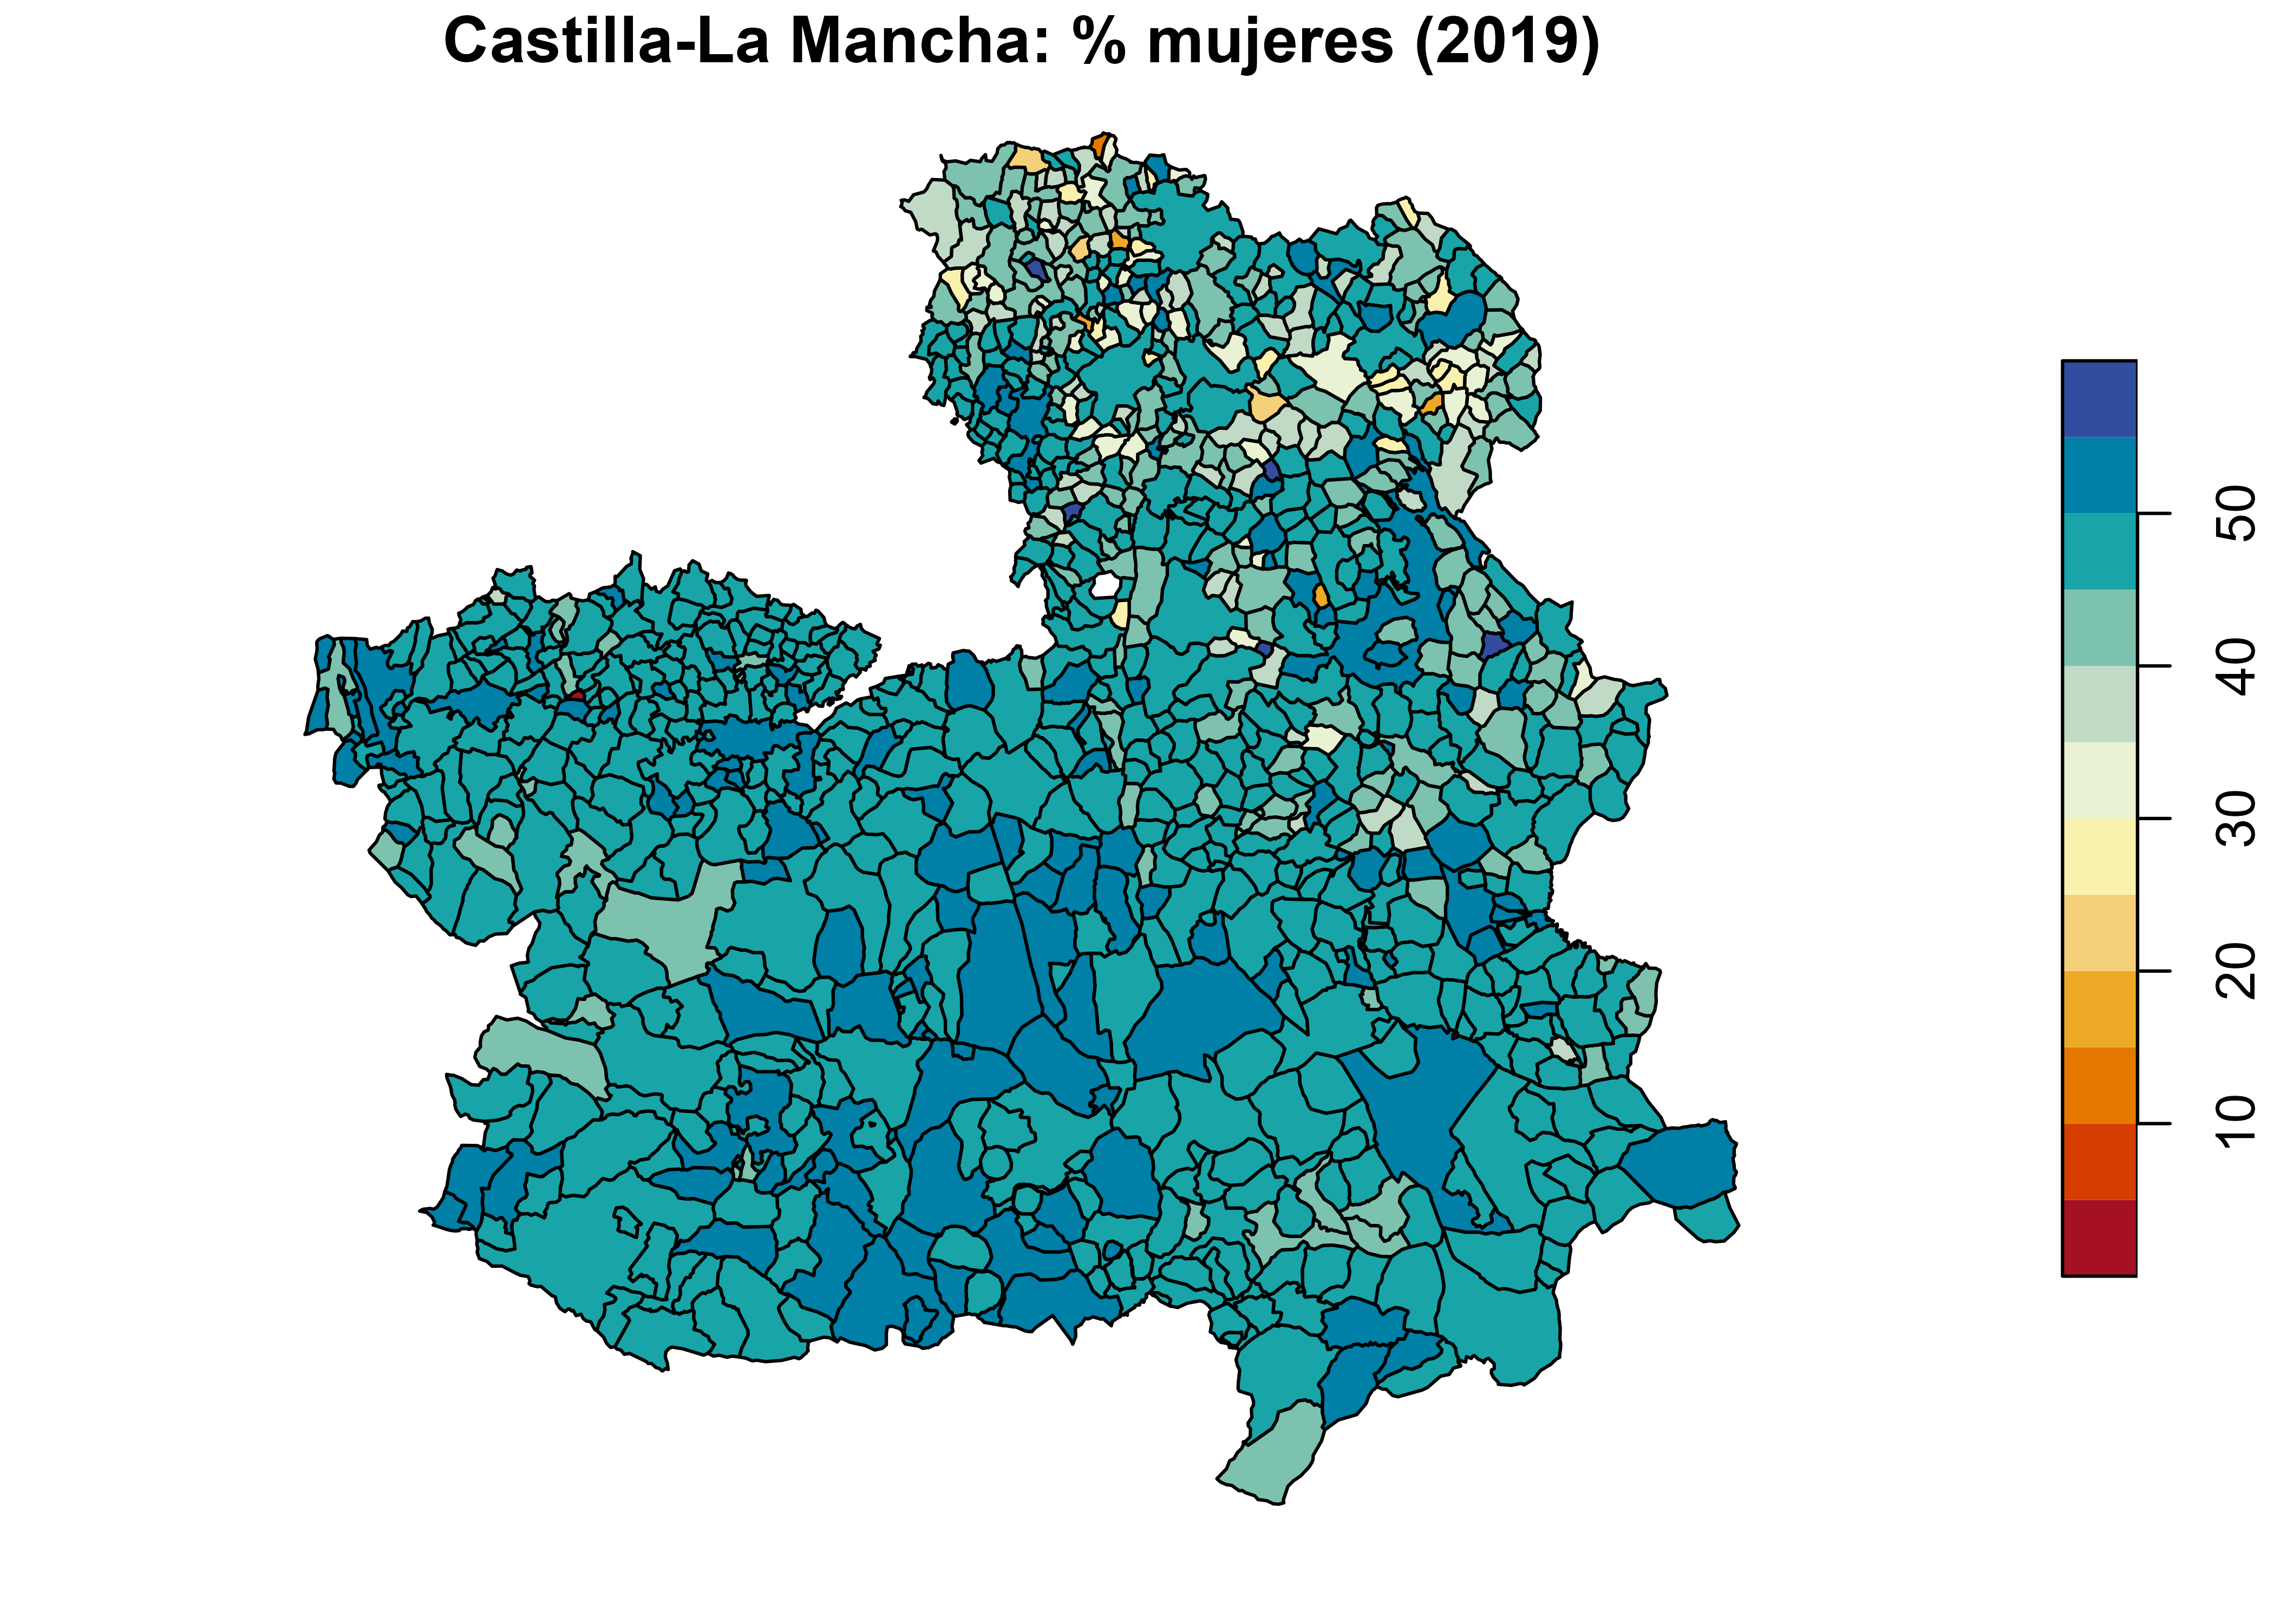
\includegraphics[width=0.6\linewidth]{_main_files/figure-latex/mapa-clm-1} 

}

\caption{Porcentaje de Mujeres en Castilla-La Mancha}\label{fig:mapa-clm}
\end{figure}

La Fig. \ref{fig:mapa-clm} presenta una serie de elementos gráficos,
característicos de los objetos espaciales:

\begin{itemize}
\item
  Los municipios de Castilla-la Mancha están representados por polígonos con
  un contorno negro y se rellenan de colores de acuerdo con la variable que
  estamos analizando, el porcentaje de mujeres en los municipios de
  Castilla-La Mancha en el año 2019.
\item
  Una leyenda explica el significado de los colores.
\item
  La variable, el porcentaje de mujeres en los municipios de Castilla-La
  Mancha en el año 2019, no parece distribuirse de manera independiente sino
  todo lo contrario, muestra un patrón espacial. Los municipios del las
  provincias Guadalajara y Cuenca (noreste) presentan tasas más bajas que los
  municipios del centro de la Comunidad.
\end{itemize}

\begin{Shaded}
\begin{Highlighting}[]
\FunctionTok{head}\NormalTok{(geo\_pob[}\StringTok{"porc\_mujeres"}\NormalTok{])}
\CommentTok{\#\textgreater{} Simple feature collection with 6 features and 1 field}
\CommentTok{\#\textgreater{} Geometry type: POLYGON}
\CommentTok{\#\textgreater{} Dimension:     XY}
\CommentTok{\#\textgreater{} Bounding box:  xmin: {-}2.18037 ymin: 38.5441 xmax: {-}1.31112 ymax: 39.35597}
\CommentTok{\#\textgreater{} Geodetic CRS:  ETRS89}
\CommentTok{\#\textgreater{}   porc\_mujeres                       geometry}
\CommentTok{\#\textgreater{} 1     52.02532 POLYGON (({-}1.58316 39.20446...}
\CommentTok{\#\textgreater{} 2     43.93064 POLYGON (({-}1.40607 39.12384...}
\CommentTok{\#\textgreater{} 3     51.14089 POLYGON (({-}2.0562 38.88697,...}
\CommentTok{\#\textgreater{} 4     48.55491 POLYGON (({-}1.54055 38.61066...}
\CommentTok{\#\textgreater{} 5     48.78419 POLYGON (({-}1.38514 39.35429...}
\CommentTok{\#\textgreater{} 6     44.49541 POLYGON (({-}2.15635 38.71074...}
\end{Highlighting}
\end{Shaded}

Antes de dibujar la Fig. \ref{fig:mapa-clm} tuvimos que leer los datos de la
librería \texttt{mapSpain} \citep{rmapspain} que contenía tanto la variable que hemos
analizado como el formato del mapa. Tras unir variable y mapa con la función
\texttt{merge()}. Al llevar a cabo un resumen del objeto espacial nos encontramos con
las siguiente información:

\begin{itemize}
\tightlist
\item
  el conjunto de datos (seleccionado) tiene 919 registros (municipios)
\item
  el tipo de geometría es POLYGON.
\item
  el CRS es ETRS89
\end{itemize}

\hypertarget{clasificaciuxf3n-de-datos-espaciales}{%
\section{Clasificación de datos espaciales}\label{clasificaciuxf3n-de-datos-espaciales}}

Tal y como acabamos de señalar y de acuerdo con \citet{Schabenberger_Gotway_2005}, p.
6), debido a que los datos espaciales surgen en una gran variedad de campos y
aplicaciones, también hay una gran variedad de tipos de datos espaciales,
estructuras y escenarios. Por tanto, una clasificación exhaustiva de los datos
espaciales sería un reto muy difícil y hemos apostado por una clasificación
general, simple y útil de datos espaciales proporcionada por \citet{cressie1993}.

La \textbf{clasificación} de Cressie de datos espaciales se basa en la naturaleza del
dominio espacial en estudio. Dependiendo de esto, podemos tener: datos
geoestadísticos, datos de patrones de puntos y datos lattice (véase Fig.
\ref{fig:hengl-cressie} en la que se han simulado los distintos procesos espaciales).

\begin{figure}

{\centering 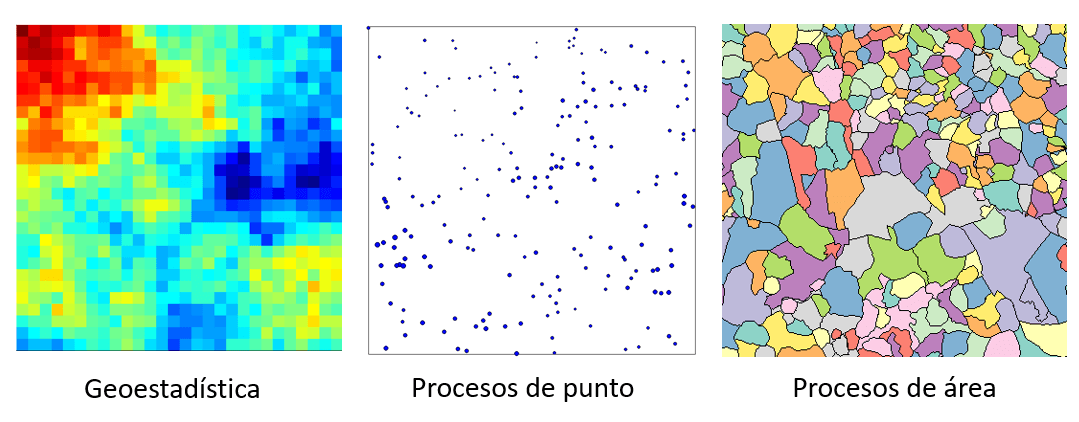
\includegraphics[width=0.6\linewidth]{img/cressie_simulados} 

}

\caption{Clasificación de datos espaciales propuesta por Cressie (1993))}\label{fig:hengl-cressie}
\end{figure}

Siguiendo a \citet{cressie1993}, sea \(s ∈ ℝ^d\) una localización en un espacio Euclideo
\(d-\)dimensional y \({Z(s)∶ s ∈ ℝ^d}\) una función aleatoria espacial, donde \(Z\)
representa el atributo en el cual estamos interesados, se tendría la siguiente
clasificación \citep{montero_et_al_2015}:

\begin{enumerate}
\def\labelenumi{\arabic{enumi}.}
\item
  \textbf{Datos geoestadísticos: }Surgen cuando el dominio de estudio es \textbf{continuo
  y fijo} \(D\). Es decir: (i) \(Z(s)\) se puede observar en cualquier punto del
  dominio (continuo); y (ii) los puntos en \(D\) no son estocásticos (son fijos,
  \(D\) es el mismo para todas las realizaciones de la función aleatoria
  espacial).

  Algunos ejemplos de datos geoestadísticos son el nivel de un contaminante en
  una ciudad, los valores de precipitación o temperatura del aire en un país,
  las concentraciones de metales pesados en la capa superior del suelo de una
  región, etc.

  Es obvio que, al menos en teoría, el nivel de un contaminante específico
  podría medirse en cualquier lugar de la ciudad; Lo mismo puede decirse de
  las mediciones de precipitaciones o temperaturas del aire en un país o
  concentraciones de un metal pesado en una región. Sin embargo, en la
  práctica, no es posible una observación exhaustiva del proceso espacial. Por
  lo general, el proceso espacial se observa en un conjunto de ubicaciones
  (por ejemplo, el nivel de un contaminante específico en una ciudad se
  observa en los puntos donde están ubicadas las estaciones de monitoreo) y,
  basado en tales valores observados, el análisis geoestadístico reproduce el
  comportamiento de el proceso espacial en todo el dominio de interés.
  La Fig. @ref(fig:ejem\_geo) presenta un mapa de interpolación krigeado del
  nivel de monoxido de carbono (CO) en logaritmos para la ciudad de Madrid.

  En el análisis geoestadístico lo más importante es cuantificar la
  correlación espacial entre observaciones (a través de la herramienta básica
  en geoestadística, el semivariograma) y utilizar esta información para
  lograr los objetivos anteriores (véase \citet{montero_et_al_2015} para un análisis
  profundo de los métodos geoestadísticos espaciales y espacio-temporales\}.
\end{enumerate}

AQUÍ ERROR, SÓLO ES UN PLOT

\begin{enumerate}
\def\labelenumi{\arabic{enumi}.}
\setcounter{enumi}{1}
\item
  \textbf{Datos reticulares}: Surgen cuando: (i) el dominio bajo estudio \(D\) es
  \textbf{discreto}, es decir, \(Z(s)\) puede observarse en una serie de ubicaciones
  fijas que pueden enumerarse. Estas ubicaciones pueden ser puntos o regiones,
  pero generalmente son códigos postales, pistas censales, vecindarios,
  provincias, países, etc., y los datos en la mayoría de los casos son datos
  agregados espacialmente sobre estas áreas. Aunque estas regiones pueden
  tener una forma regular, normalmente la forma que tienen es irregular, y
  esto, junto con el carácter espacialmente agregado de la datos, es por lo
  que los datos latice tambien se denominan datos regionales. Y (ii) las
  ubicaciones en \(D\) no son estocásticas. Por supuesto, un concepto clave en
  el análisis de los datos lattice es el \textbf{vecindario} y la matriz \textbf{W}.

  Algunos ejemplos de reticulares incluyen la tasa de desempleo por estados,
  los datos de delincuencia por comarcas, rendimientos agrícolas en parcelas,
  precios medios de la vivienda por provincias, etc. En este sentido un ejemplo
  ilustrativo se presenta en la la Fig. \ref{fig:ejem-lattice},
  que muestra la distribución municipal de la renta
  neta media por hogar en 2017 en España.
\end{enumerate}

\begin{figure}

{\centering 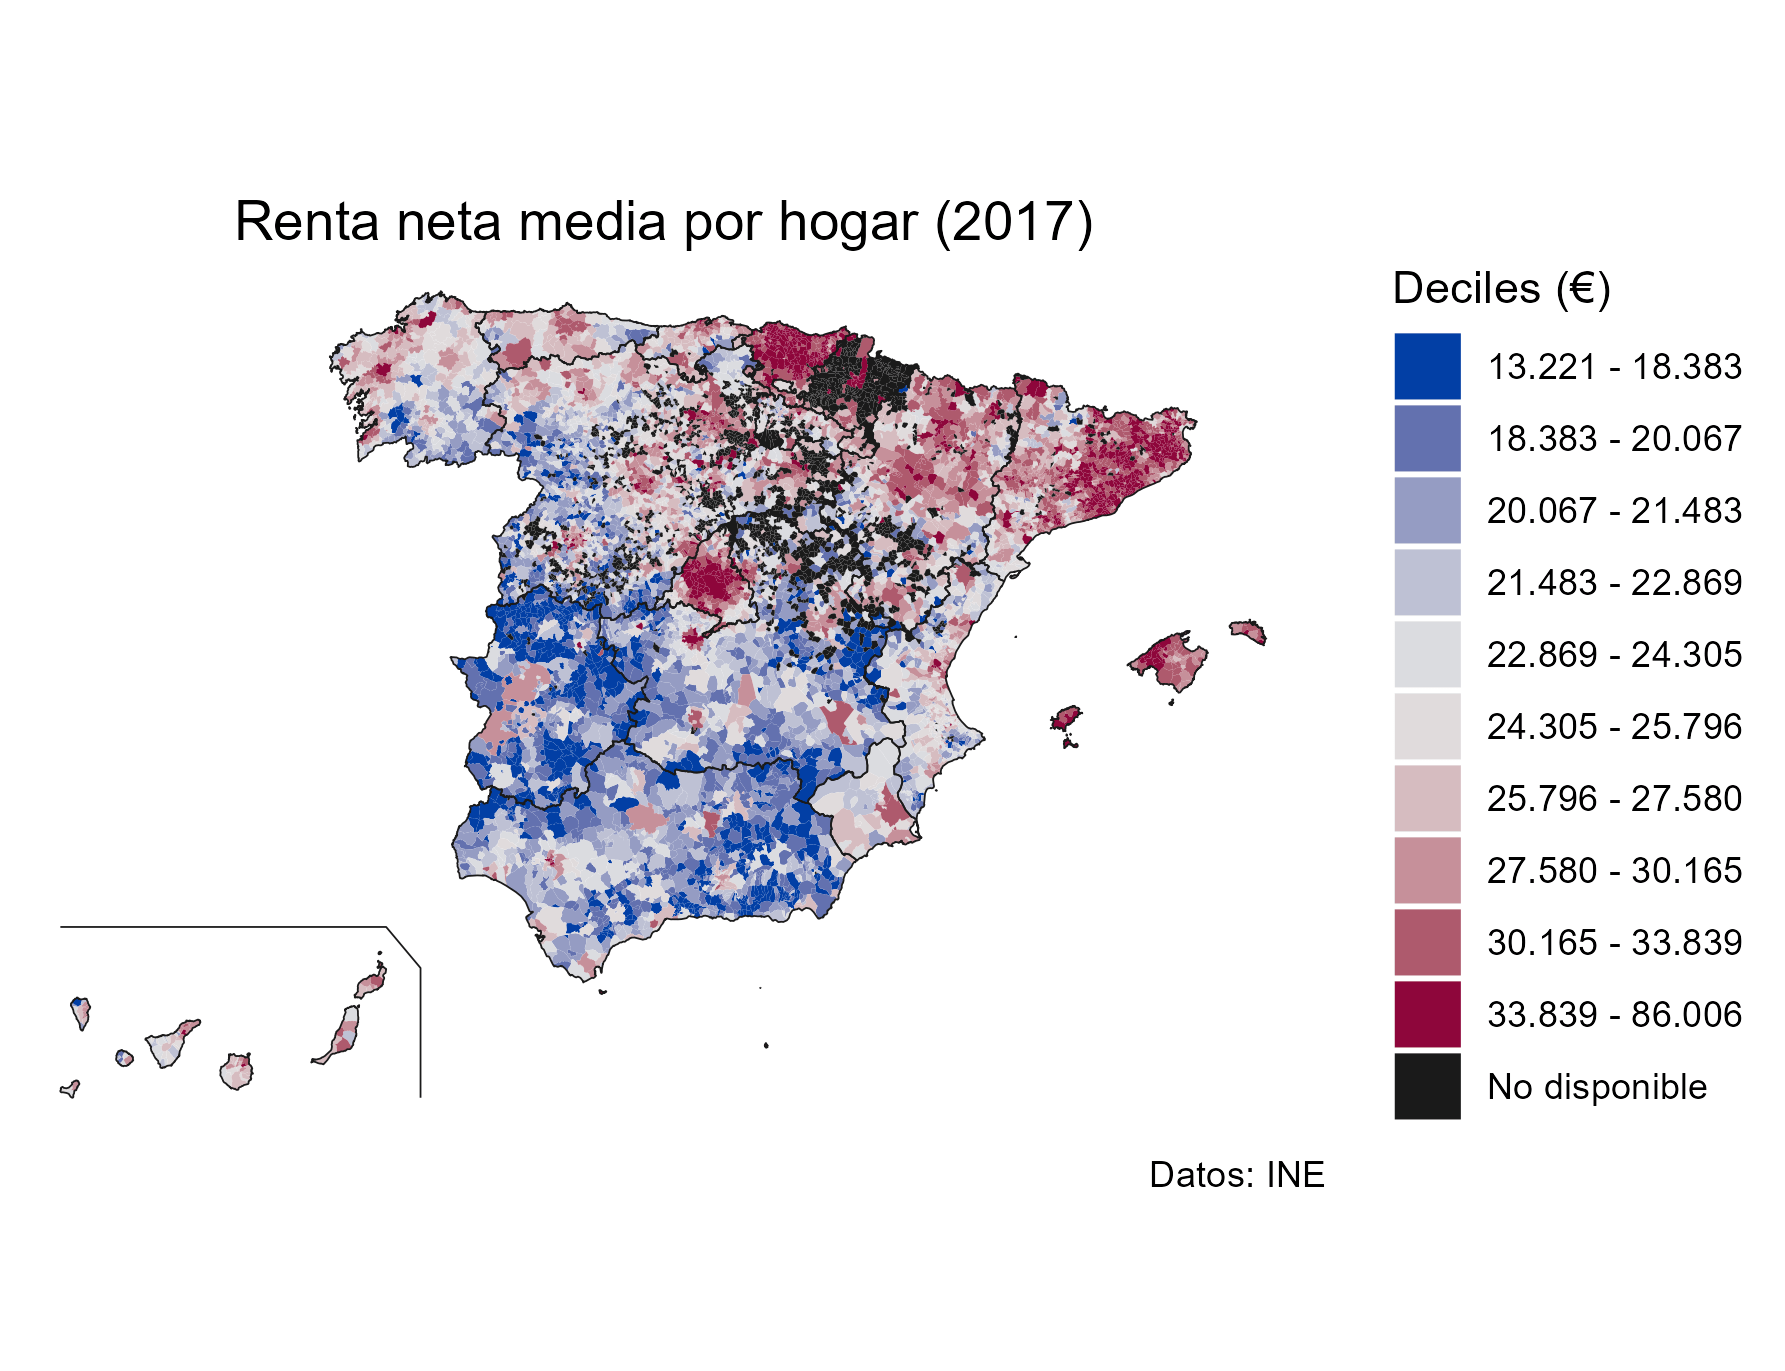
\includegraphics[width=0.6\linewidth]{img/renta2017} 

}

\caption{Renta neta media municipal española en 2017}\label{fig:ejem-lattice}
\end{figure}

\begin{enumerate}
\def\labelenumi{\arabic{enumi}.}
\setcounter{enumi}{2}
\item
  \textbf{Procesos de puntos:} Mientras que en los datos geoestadísticos y
  reticulares el dominio \(D\) es fijo, en los datos de patrones puntuales el
  dominio es discreto o continuo, pero \textbf{aleatorio}. Los patrones de puntos
  surgen cuando el atributo bajo estudio es la ubicación de los eventos
  (observaciones). Es decir, el interés radica en dónde ocurren eventos de
  interés.

  Algunos ejemplos de patrones de puntos son la ubicación de incendios en una
  región española, la ubicación de los árboles en un bosque o la ubicación de
  nidos en una colonia de aves reproductoras, la localización de los
  accidentes de tráfico en una ciudad o área de referencia,
  la localización de los delitos en una ciudad, entre muchas otras.

  En estos En los casos, es obvio que \(D\) es aleatorio y los puntos de
  observación no dependen del investigador. El principal objetivo del análisis
  de patrones de puntos es determinar si la ubicación de los eventos tiende a
  exhibir un patrón sistemático sobre el área en estudio o, por el contrario,
  son aleatoriamente repartido.

  Más concretamente, nos interesa analizar si la ubicación de los eventos es
  completamente aleatorio espacialmente (la ubicación donde ocurren los
  eventos no se ve afectada por la ubicación de otros eventos), uniforme o
  regular (cada punto está tan lejos de todos sus vecinos como sea posible) o
  agrupados o agregados (la ubicación de los eventos se concentra en grupos).
  La Fig. \ref{fig:ejem-pp} muestra la localización de los accidentes de tráfico
  registrados en la ciudad de Madrid durante el mes de febreo de 2020.
\end{enumerate}

\begin{figure}

{\centering 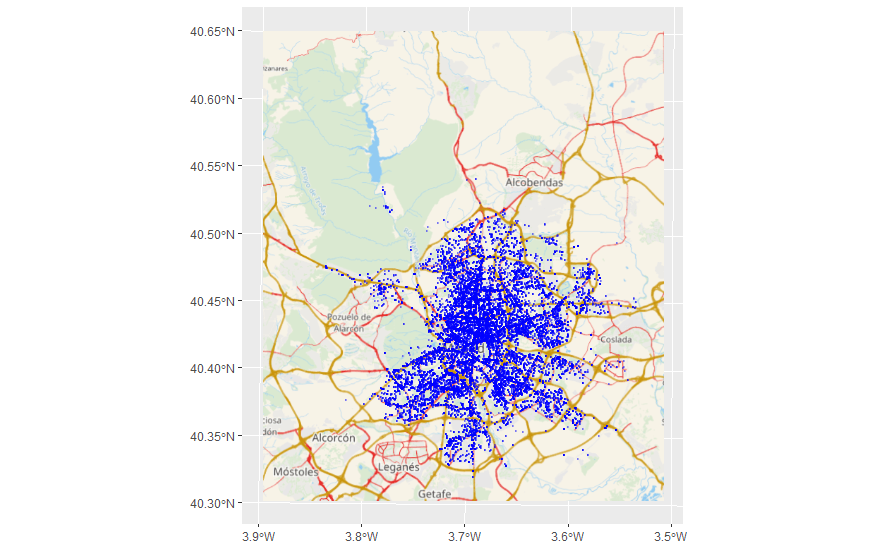
\includegraphics[width=0.6\linewidth]{img/traf_madrid_feb_2020} 

}

\caption{Accidentes de tráfico registrados en la ciudad de Madrid (Febrero de 2020)}\label{fig:ejem-pp}
\end{figure}

\hypertarget{caos}{%
\chapter{Casos prácticos}\label{caos}}

DIEGO, EN EL CSS SE PUEDE AÑADIR UN CUADRO QUE SEA UNA ADVERTENCIA, YO NO SÉ,
lO PROBAMOS/PRUEBAS :) O NO??

\hypertarget{caso-1-temperatura-muxednimas-del-aire-en-espauxf1a.}{%
\section{Caso 1: Temperatura mínimas del aire en España.}\label{caso-1-temperatura-muxednimas-del-aire-en-espauxf1a.}}

\textbf{Objetivo de aprendizaje}

Esta sección presenta un caso de uso en el que aprenderemos a realizar las
siguientes tareas básicas:

\begin{enumerate}
\def\labelenumi{\arabic{enumi}.}
\item
  Peer datos espaciales en R.
\item
  Proyectar datos espaciales.
\item
  Graficar datos espaciales.
\end{enumerate}

Para ello, se va a trabajar con los datos de temperatura mínima registradas en España
por las estaciones metereológicas de la Agencia Estatal de Meteorología (AEMET).
Un conjuto de datos ya depurados y listos par trabajar se encuentra en el fichero \texttt{tempmin.csv}.
Por otra parte, la inforación relativa al mapeo de España se obtendrá directamente
de la librería \texttt{mapSpain}.
Todo el análisis se va a realizar empleando RStudio, por lo que se empezará
abriendo el programa y creando un nuevo proyecto.

\begin{exercise}[Creación del proyecto]
\protect\hypertarget{exr:ex-crea}{}\label{exr:ex-crea}Cree un proyecto para trabajar todo lo referente al caso.
\end{exercise}

\begin{solution}
Para crear un proyecto siga la secuencia:
\emph{File\textgreater{} New Proyect\textgreater{} New File\textgreater{} RMD}
\end{solution}

El conjunto de datos proporcionado \texttt{tempmin.csv} contiene el nivel de
temperatura del aire en España entre el 6 y el 10 de Enero de
2021\footnote{Las fechas seleccionadas coinciden con el periodo en el que
  la tormenta Filomena tuvo su auge en la Península Ibérica.}. Estos datos han sido descargados usando la librería
\texttt{climaemet} \citep{R-climaemet} y han sido posteriormente tratados para su uso en
esta práctica.

El primer paso consiste en importar la base de datos de temperatura mínima. El
archivo está en formato csv, por lo cual, es un fichero de texto plano.
Se pueden usar varias funciones para realizar la importación.
Se emplara´na los paquetes del \texttt{tidyverse} para realizar
todo el tratamiento de datos.

\begin{exercise}[Importación de los datos]
\protect\hypertarget{exr:ex2}{}\label{exr:ex2}Importe los datos \texttt{tempmin.csv} y guárdelos en un objeto llamado \texttt{tmin}.
\end{exercise}

\begin{solution}

\begin{Shaded}
\begin{Highlighting}[]
\CommentTok{\# Cada uno debe seleccionar el directorio donde tiene los datos, de ahí}
\CommentTok{\# que sea conveniente trabajar con proyectos.}
\FunctionTok{library}\NormalTok{(readr)}
\NormalTok{tmin }\OtherTok{\textless{}{-}} \FunctionTok{read\_csv}\NormalTok{(}\StringTok{"data/tempmin.csv"}\NormalTok{)}
\end{Highlighting}
\end{Shaded}

\end{solution}

Los el conjunto de datos \texttt{tempmin} es un data frame que
contiene 5 variables:

\begin{itemize}
\item
  \texttt{fecha}: Indicando la fecha de observación.
\item
  \texttt{indicativo}: Es el identificador de la estación de la AEMET que registró el
  dato.
\item
  \texttt{tmin}: Dato de temperatura mínima registrada en cada fecha por la estación
  correspondiente en grados centígrados.
\item
  \texttt{longitud,\ latitud}: Coordenadas geográficas de la estación
\end{itemize}

\begin{exercise}[Descripción de los datos]
\protect\hypertarget{exr:ex3}{}\label{exr:ex3}Con la función \texttt{head()} describa, en forma de tabla, la información
que contiene el objeto \texttt{tmin} y compruebe que se corresponde con la descrita.
\end{exercise}

\begin{Shaded}
\begin{Highlighting}[]
\NormalTok{knitr}\SpecialCharTok{::}\FunctionTok{kable}\NormalTok{(}\FunctionTok{head}\NormalTok{(tmin), }\AttributeTok{caption =} \StringTok{"Detalle del objeto tmin"}\NormalTok{)}
\end{Highlighting}
\end{Shaded}

\begin{table}

\caption{\label{tab:tmin-head}Detalle del objeto tmin}
\centering
\begin{tabular}[t]{l|l|r|r|r}
\hline
fecha & indicativo & tmin & longitud & latitud\\
\hline
2021-01-06 & 4358X & -4.7 & -5.880556 & 38.95556\\
\hline
2021-01-06 & 4220X & -7.0 & -4.616389 & 39.08861\\
\hline
2021-01-06 & 6106X & 4.7 & -4.748333 & 37.02944\\
\hline
2021-01-06 & 9698U & -6.8 & 0.865278 & 42.20528\\
\hline
2021-01-06 & 4410X & -3.4 & -6.385556 & 38.91583\\
\hline
2021-01-06 & 1331A & 1.0 & -7.031389 & 43.52472\\
\hline
\end{tabular}
\end{table}

Una de las clases de objetos espaciales más utilzada en R es \texttt{sf}. Sin embargo,
dependiendo del análisis que se quiera realizar hay otras muy comunes como
\texttt{geodata}, \texttt{spatastat}, etc..

A continuación se convertirá el objeto \texttt{tmin} (\texttt{data.frame})
a un objeto de la clase \texttt{geodata}, una clase muy utilizada para trabajar con
datos espacilaes y requerida por la librería \texttt{geoR}.
Estos objetos contienen las coordenadas y la variable objeto de estudio.
Para mayor detalle ver \texttt{??as.geodata}. Obsérvese como varía la variable
a través de los ejes longitud y latitud. Observe tambien la forma campaniforme
de la distribución de la variale.

\begin{exercise}[Descripción de los datos]
\protect\hypertarget{exr:ex4}{}\label{exr:ex4}Del objeto \texttt{tmin} seleccione el día \textbf{8 de enero de 2022}
y las variables \texttt{longitud}, \texttt{latitud} y \texttt{tmin} para crear el objeto
y llámelo \texttt{tmin\_geoR}. A continuación describa analítica y
gráficamente dicho objeto.
\end{exercise}

\begin{Shaded}
\begin{Highlighting}[]
\FunctionTok{library}\NormalTok{(dplyr)}
\FunctionTok{library}\NormalTok{(geoR)}

\NormalTok{tmin\_geoR }\OtherTok{\textless{}{-}}\NormalTok{ tmin }\SpecialCharTok{\%\textgreater{}\%}
  \FunctionTok{filter}\NormalTok{(fecha }\SpecialCharTok{==} \StringTok{"2021{-}01{-}08"}\NormalTok{) }\SpecialCharTok{\%\textgreater{}\%}
  \CommentTok{\# Seleccionamos las columnas de interés}
\NormalTok{  dplyr}\SpecialCharTok{::}\FunctionTok{select}\NormalTok{(longitud, latitud, tmin) }\SpecialCharTok{\%\textgreater{}\%}
  \CommentTok{\# Y creamos el objeto geodata}
  \FunctionTok{as.geodata}\NormalTok{(}
    \AttributeTok{coords.col =} \DecValTok{1}\SpecialCharTok{:}\DecValTok{2}\NormalTok{,}
    \AttributeTok{data.col =} \DecValTok{3}
\NormalTok{  )}


\FunctionTok{summary}\NormalTok{(tmin\_geoR)}
\CommentTok{\#\textgreater{} Number of data points: 211 }
\CommentTok{\#\textgreater{} }
\CommentTok{\#\textgreater{} Coordinates summary}
\CommentTok{\#\textgreater{}      longitud  latitud}
\CommentTok{\#\textgreater{} min {-}9.291389 35.27639}
\CommentTok{\#\textgreater{} max  4.215556 43.78611}
\CommentTok{\#\textgreater{} }
\CommentTok{\#\textgreater{} Distance summary}
\CommentTok{\#\textgreater{}         min         max }
\CommentTok{\#\textgreater{}  0.01024389 13.85144264 }
\CommentTok{\#\textgreater{} }
\CommentTok{\#\textgreater{} Data summary}
\CommentTok{\#\textgreater{}        Min.     1st Qu.      Median        Mean     3rd Qu.        Max. }
\CommentTok{\#\textgreater{} {-}14.9000000  {-}4.6000000  {-}0.5000000  {-}0.6293839   3.5000000  13.6000000}
\FunctionTok{plot}\NormalTok{(tmin\_geoR)}
\end{Highlighting}
\end{Shaded}

\begin{figure}

{\centering 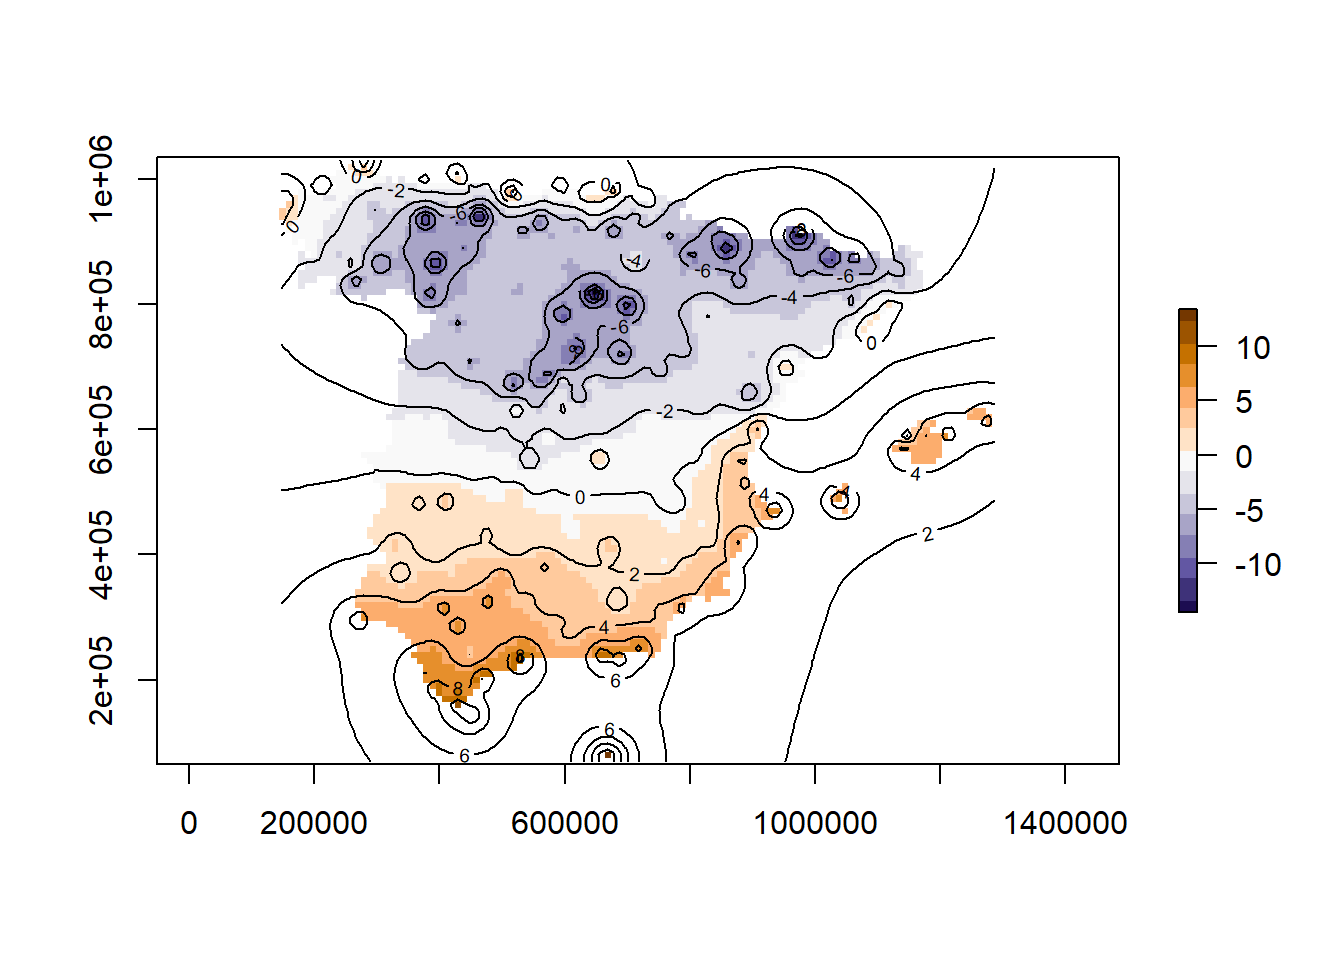
\includegraphics[width=0.6\linewidth]{_main_files/figure-latex/unnamed-chunk-9-1} 

}

\caption{Convertir `data.frame` a `geodata`}\label{fig:unnamed-chunk-9}
\end{figure}

En esta ocasión, convertiremos los datos de \texttt{tmin} en un objeto espacial \texttt{sf}, es
decir, datos espaciales de tipo vector.

Los datos de \texttt{tmin} contienen coordenadas geográficas longitud/latitud, así que
como se vió en la Sección \textbf{Sistema de Referencia de Coordenadas (CRS)} el CRS a
emplear ha de ser un CRS geográfico. Usaremos el código EPSG \textbf{4326}, que
corresponde a coordenadas geográficas y suele ser el habitual en este tipo de
situaciones.

\begin{exercise}[Convertir `data.frame` a `sf`]
\protect\hypertarget{exr:ex5}{}\label{exr:ex5}Del objeto \texttt{tmin} seleccione las variables \texttt{longitud}, \texttt{latitud} y \texttt{tmin}
para crear el objeto sf y llámelo \texttt{tmin\_sf}.
A continuación describa el objeto creado.
\end{exercise}

\begin{Shaded}
\begin{Highlighting}[]
\FunctionTok{library}\NormalTok{(sf)}

\NormalTok{tmin\_sf }\OtherTok{\textless{}{-}} \FunctionTok{st\_as\_sf}\NormalTok{(tmin,}
  \AttributeTok{coords =} \FunctionTok{c}\NormalTok{(}\StringTok{"longitud"}\NormalTok{, }\StringTok{"latitud"}\NormalTok{),}
  \AttributeTok{crs =} \DecValTok{4326}
\NormalTok{)}

\NormalTok{tmin\_sf}
\CommentTok{\#\textgreater{} Simple feature collection with 1066 features and 3 fields}
\CommentTok{\#\textgreater{} Geometry type: POINT}
\CommentTok{\#\textgreater{} Dimension:     XY}
\CommentTok{\#\textgreater{} Bounding box:  xmin: {-}9.291389 ymin: 35.27639 xmax: 4.215556 ymax: 43.78611}
\CommentTok{\#\textgreater{} Geodetic CRS:  WGS 84}
\CommentTok{\#\textgreater{} \# A tibble: 1,066 x 4}
\CommentTok{\#\textgreater{}    fecha      indicativo  tmin             geometry}
\CommentTok{\#\textgreater{}  * \textless{}date\textgreater{}     \textless{}chr\textgreater{}      \textless{}dbl\textgreater{}          \textless{}POINT [°]\textgreater{}}
\CommentTok{\#\textgreater{}  1 2021{-}01{-}06 4358X       {-}4.7 ({-}5.880556 38.95556)}
\CommentTok{\#\textgreater{}  2 2021{-}01{-}06 4220X       {-}7   ({-}4.616389 39.08861)}
\CommentTok{\#\textgreater{}  3 2021{-}01{-}06 6106X        4.7 ({-}4.748333 37.02944)}
\CommentTok{\#\textgreater{}  4 2021{-}01{-}06 9698U       {-}6.8  (0.865278 42.20528)}
\CommentTok{\#\textgreater{}  5 2021{-}01{-}06 4410X       {-}3.4 ({-}6.385556 38.91583)}
\CommentTok{\#\textgreater{}  6 2021{-}01{-}06 1331A        1   ({-}7.031389 43.52472)}
\CommentTok{\#\textgreater{}  7 2021{-}01{-}06 1690A       {-}0.1 ({-}7.859722 42.32528)}
\CommentTok{\#\textgreater{}  8 2021{-}01{-}06 8489X       {-}8   ({-}0.255833 40.43333)}
\CommentTok{\#\textgreater{}  9 2021{-}01{-}06 8025         2    ({-}0.494167 38.3725)}
\CommentTok{\#\textgreater{} 10 2021{-}01{-}06 9784P      {-}10       (0.224722 42.63)}
\CommentTok{\#\textgreater{} \# ... with 1,056 more rows}
\end{Highlighting}
\end{Shaded}

La siguiente tarea será representar las estaciones que monitorizan
la temperatura mínima en un mapa de España.

\begin{exercise}[Reprsentación espacial de la clase sf]
\protect\hypertarget{exr:ex6}{}\label{exr:ex6}Represente un mapa de ESpaña, con las Comunidades Autónomas de incluidas,
excepto las Islas Canarias (por simplicidad)
\end{exercise}

\begin{solution}

Una opción es utilizar un paquete API que nos proporciona esta información
en formato \texttt{sf}, el paquete \texttt{mapSpain}.

\begin{Shaded}
\begin{Highlighting}[]
\FunctionTok{library}\NormalTok{(mapSpain)}
\CommentTok{\# sf object}
\NormalTok{esp }\OtherTok{\textless{}{-}} \FunctionTok{esp\_get\_ccaa}\NormalTok{() }\SpecialCharTok{\%\textgreater{}\%}
  \CommentTok{\# No vamos a usar Canarias en este análisis}
  \FunctionTok{filter}\NormalTok{(ine.ccaa.name }\SpecialCharTok{!=} \StringTok{"Canarias"}\NormalTok{)}


\FunctionTok{plot}\NormalTok{(esp}\SpecialCharTok{$}\NormalTok{geometry) }\CommentTok{\# Dibujamo el mapa de España menos las Islas Canarias}
\end{Highlighting}
\end{Shaded}

\begin{figure}

{\centering 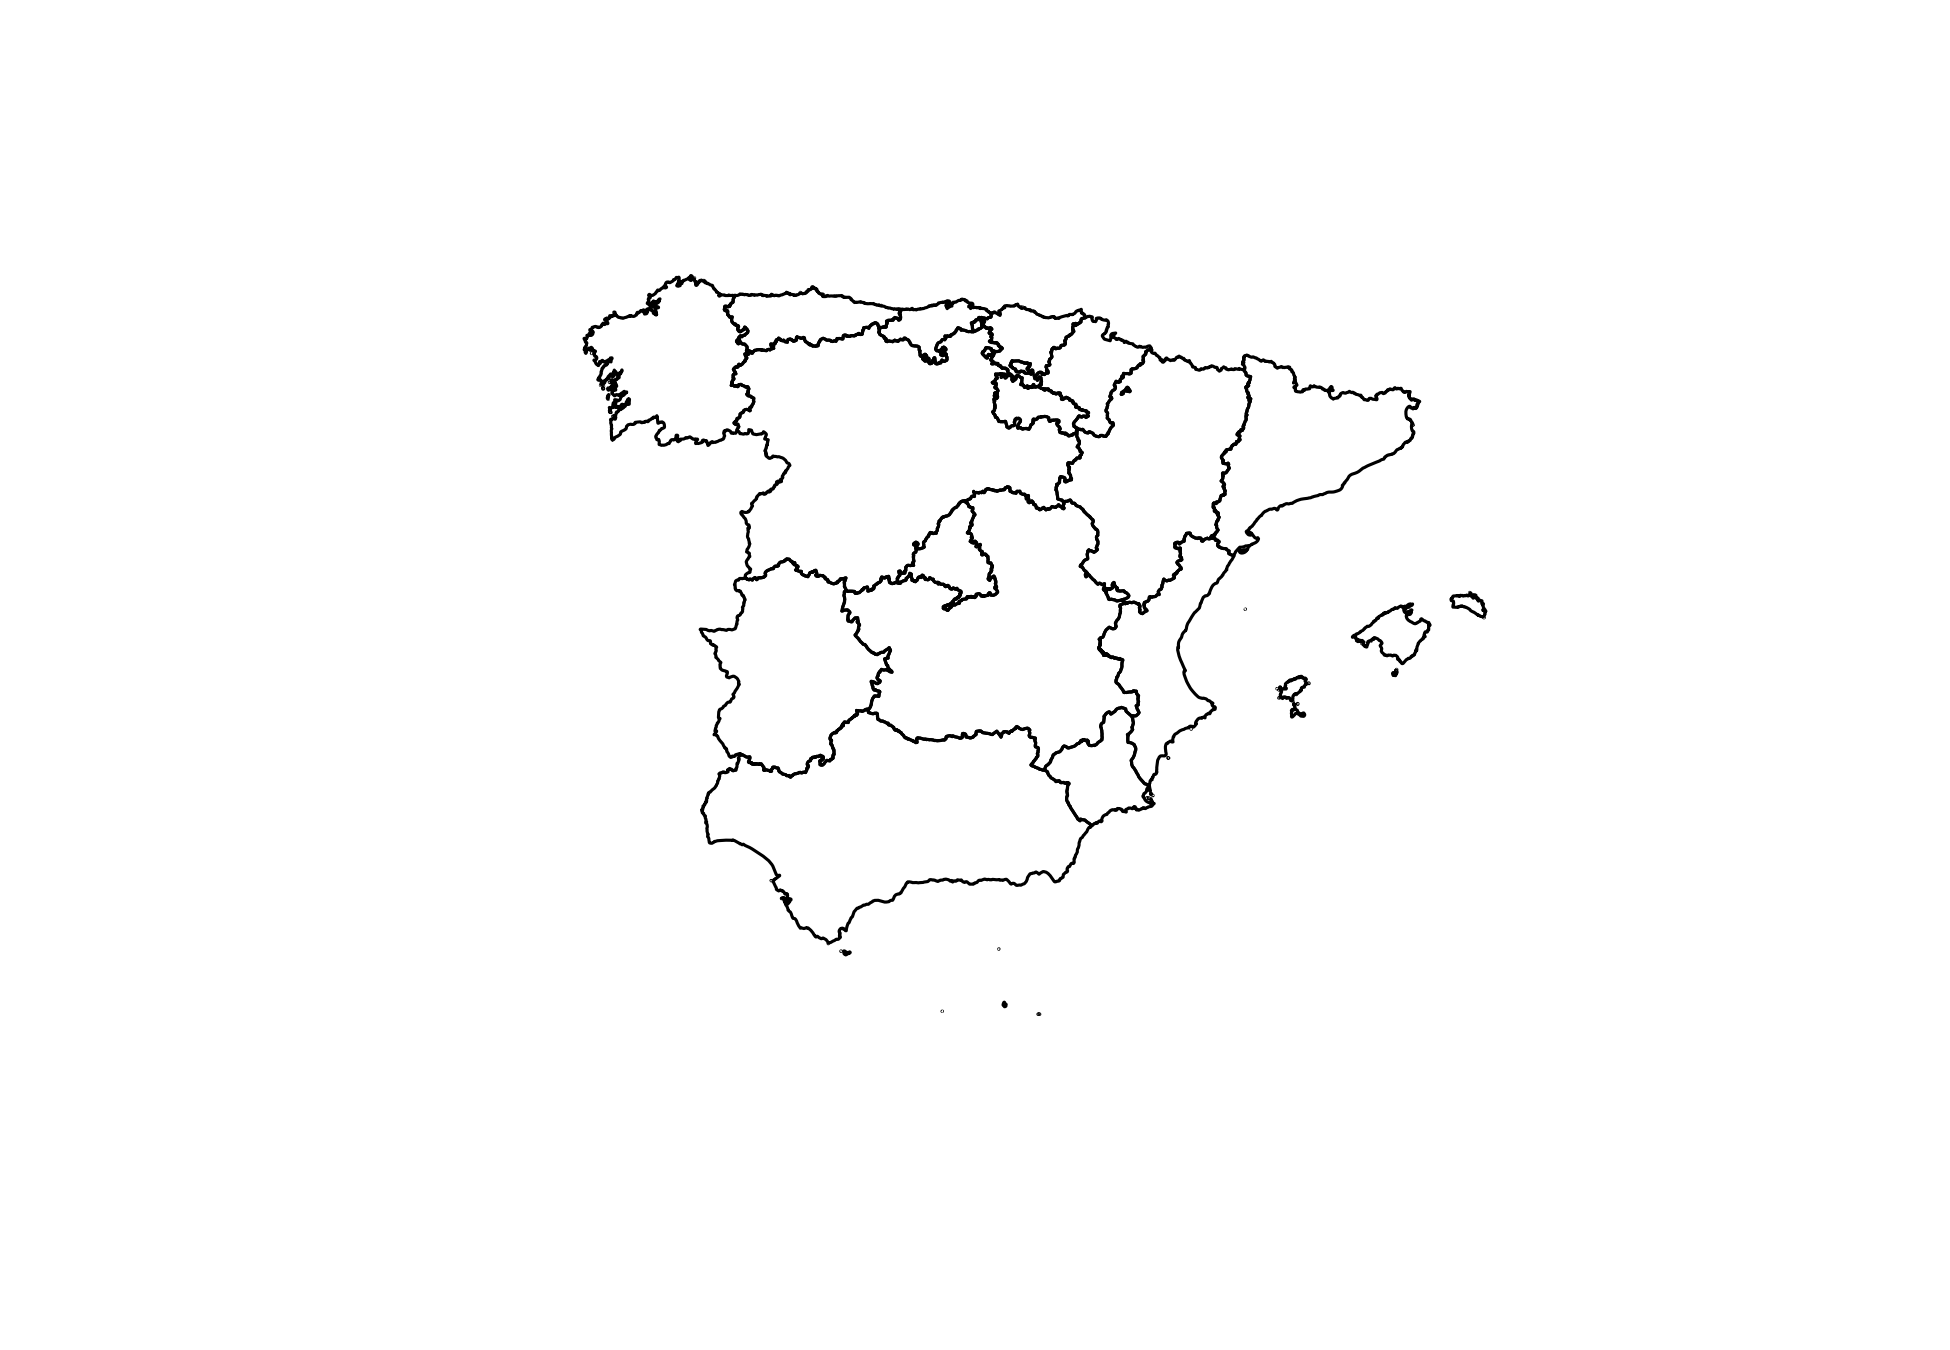
\includegraphics[width=0.6\linewidth]{_main_files/figure-latex/unnamed-chunk-11-1} 

}

\caption{Mapa de España (Sin Canarias)}\label{fig:unnamed-chunk-11}
\end{figure}

\end{solution}

Como se comentó en la sección \textbf{Sistema de Referencia de Coordenadas (CRS)},
cuando se emplean datos geográficos provenientes de varias fuentes, es necesario
asegurarse de que ambos objetos están usando el mismo CRS.

\begin{exercise}[CRS]
\protect\hypertarget{exr:ex7}{}\label{exr:ex7}¿Tengo el Sistema de referencia de coordenadas (CRS) de las estaciones de
monitoreo en la misma proyección que el contorno de España? Compruebelo.
\end{exercise}

\begin{Shaded}
\begin{Highlighting}[]
\FunctionTok{st\_crs}\NormalTok{(tmin\_sf) }\SpecialCharTok{==} \FunctionTok{st\_crs}\NormalTok{(esp)}
\CommentTok{\#\textgreater{} [1] FALSE}
\end{Highlighting}
\end{Shaded}

Se ha comprobado que no lo están, por lo que hay que proyectar las coordenadas a un CRS
común.

\begin{exercise}[CRS]
\protect\hypertarget{exr:ex8}{}\label{exr:ex8}Proyecte las coordenadas de los objetos \texttt{tmin\_sf} y \texttt{esp}
al CRS de referencia de \texttt{tmin\_sf}. Compruébelo.
\end{exercise}

\begin{Shaded}
\begin{Highlighting}[]
\NormalTok{esp2 }\OtherTok{\textless{}{-}} \FunctionTok{st\_transform}\NormalTok{(esp, }\FunctionTok{st\_crs}\NormalTok{(tmin\_sf))}

\FunctionTok{st\_crs}\NormalTok{(tmin\_sf) }\SpecialCharTok{==} \FunctionTok{st\_crs}\NormalTok{(esp2)}
\CommentTok{\#\textgreater{} [1] TRUE}
\end{Highlighting}
\end{Shaded}

Para dibujar las estaciones de monitoreo con el contorno de España, existen
varias opciones de paquetes, \texttt{ggplot2} (paquete de referencia en representaciones
gráficas), \texttt{tmap} o \texttt{mapsf} (estos dos
últimos especializados en mapas temáticos,)

paquete \texttt{ggplot2} como referencia, sin embargo existen varios paquetes

\begin{exercise}[CRS]
\protect\hypertarget{exr:ex9}{}\label{exr:ex9}Represente, con el paquete \texttt{ggplot2}, las estaciones de monitorero de AEMET
en la península Ibérica.
\end{exercise}

\begin{Shaded}
\begin{Highlighting}[]
\FunctionTok{library}\NormalTok{(ggplot2)}

\FunctionTok{ggplot}\NormalTok{(esp2) }\SpecialCharTok{+}
  \CommentTok{\# Para graficar objetos sf debemos usar geom\_sf()}
  \FunctionTok{geom\_sf}\NormalTok{() }\SpecialCharTok{+}
  \FunctionTok{geom\_sf}\NormalTok{(}\AttributeTok{data =}\NormalTok{ tmin\_sf) }\SpecialCharTok{+}
  \FunctionTok{theme\_light}\NormalTok{() }\SpecialCharTok{+}
  \CommentTok{\# labs(}
  \CommentTok{\#  title = "Estaciones de monitoreo AEMET en  España",}
  \CommentTok{\#  subtitle = "excluyendo las Islas Canarias"}
  \CommentTok{\# ) +}
  \FunctionTok{theme}\NormalTok{(}
    \AttributeTok{plot.title =} \FunctionTok{element\_text}\NormalTok{(}
      \AttributeTok{size =} \DecValTok{12}\NormalTok{,}
      \AttributeTok{face =} \StringTok{"bold"}
\NormalTok{    ),}
    \AttributeTok{plot.subtitle =} \FunctionTok{element\_text}\NormalTok{(}
      \AttributeTok{size =} \DecValTok{8}\NormalTok{,}
      \AttributeTok{face =} \StringTok{"italic"}
\NormalTok{    )}
\NormalTok{  )}
\end{Highlighting}
\end{Shaded}

\begin{figure}

{\centering 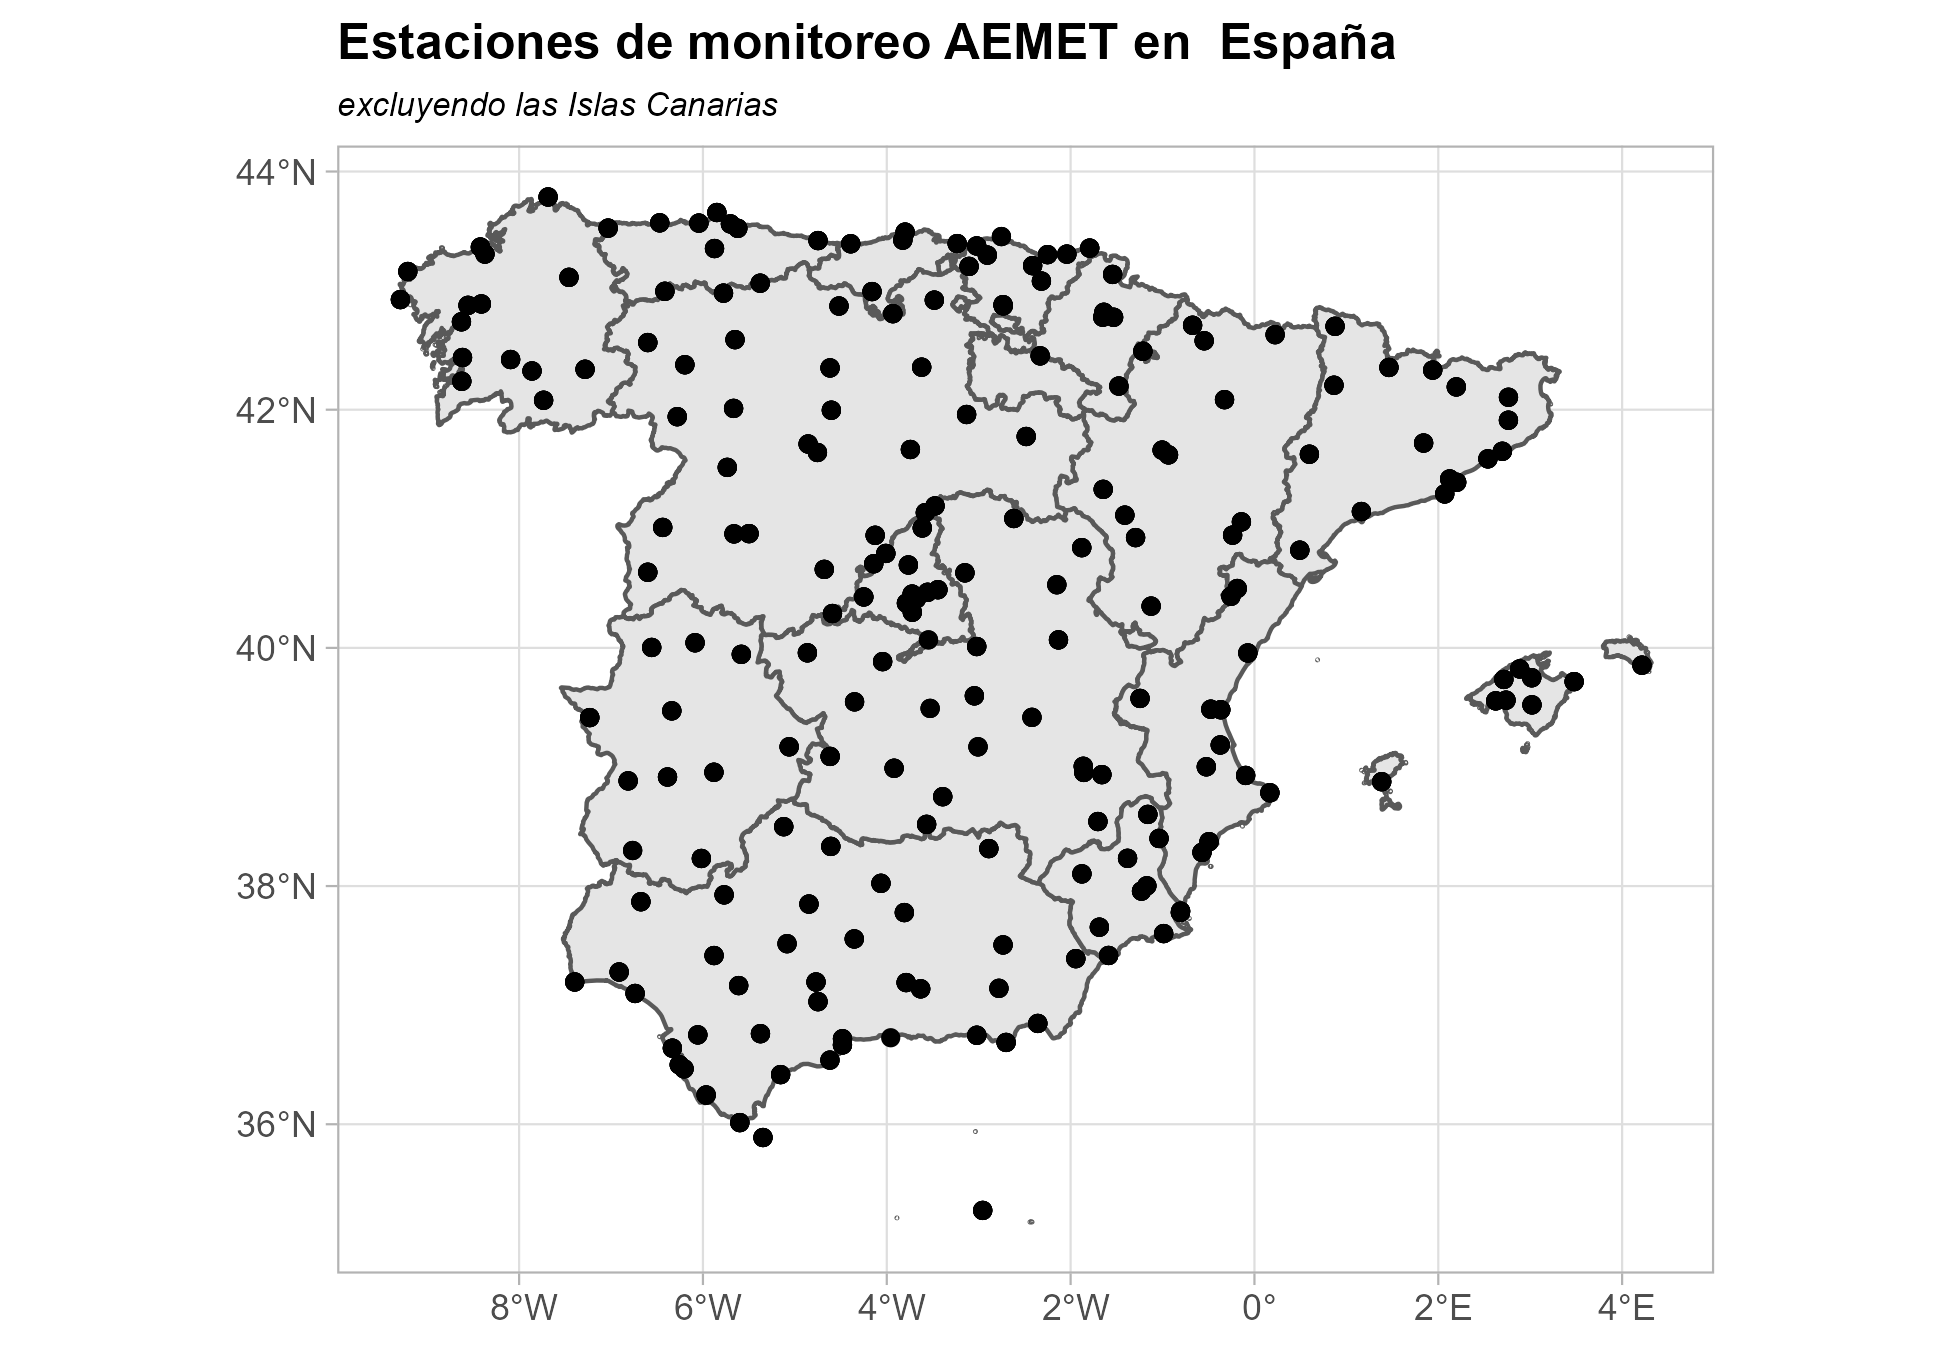
\includegraphics[width=0.6\linewidth]{_main_files/figure-latex/unnamed-chunk-13-1} 

}

\caption{Estaciones de AEMET en la Península Ibérica}\label{fig:unnamed-chunk-13}
\end{figure}

Una vez represtadas las coordenadas, es decir, las estaciones de monitoreo dónde se ha medido la variable
temperatura mínima \texttt{tmin}, el siguiente paso será representar el valor que toma
la variable en esas coodenadas. La base \texttt{tmin} contine informaicón temporal
para para varios días, por lo que, como este análisis es meramente espacial
se elegirá un día que se fijará para todo el análisis.

\begin{exercise}[plot-sp1]
\protect\hypertarget{exr:ex10}{}\label{exr:ex10}Representamos la variable temperatura mínima \texttt{tmin} para el día \textbf{8 de
enero de 2021}. Gurarde la base de datos espacial para ese día en un objeto
de nombre \texttt{tmin\_8enero}.
\end{exercise}

\begin{Shaded}
\begin{Highlighting}[]

\CommentTok{\# Seleccionaremos los datos correspondientes al 8 de enero de 2021}
\NormalTok{tmin\_8enero }\OtherTok{\textless{}{-}}\NormalTok{ tmin\_sf }\SpecialCharTok{\%\textgreater{}\%}
  \FunctionTok{filter}\NormalTok{(fecha }\SpecialCharTok{==} \StringTok{"2021{-}01{-}08"}\NormalTok{)}


\CommentTok{\# Mapa temático en el que se representan los valores de temperatura mínima}
\CommentTok{\# registrados en cada estación mediante un código de colores}
\FunctionTok{plot}\NormalTok{(tmin\_8enero[}\StringTok{"tmin"}\NormalTok{],}
  \CommentTok{\# main = "Temperatura mínima (8{-}enero{-}2021)",}
  \AttributeTok{pch =} \DecValTok{8}
\NormalTok{)}
\end{Highlighting}
\end{Shaded}

\begin{figure}

{\centering 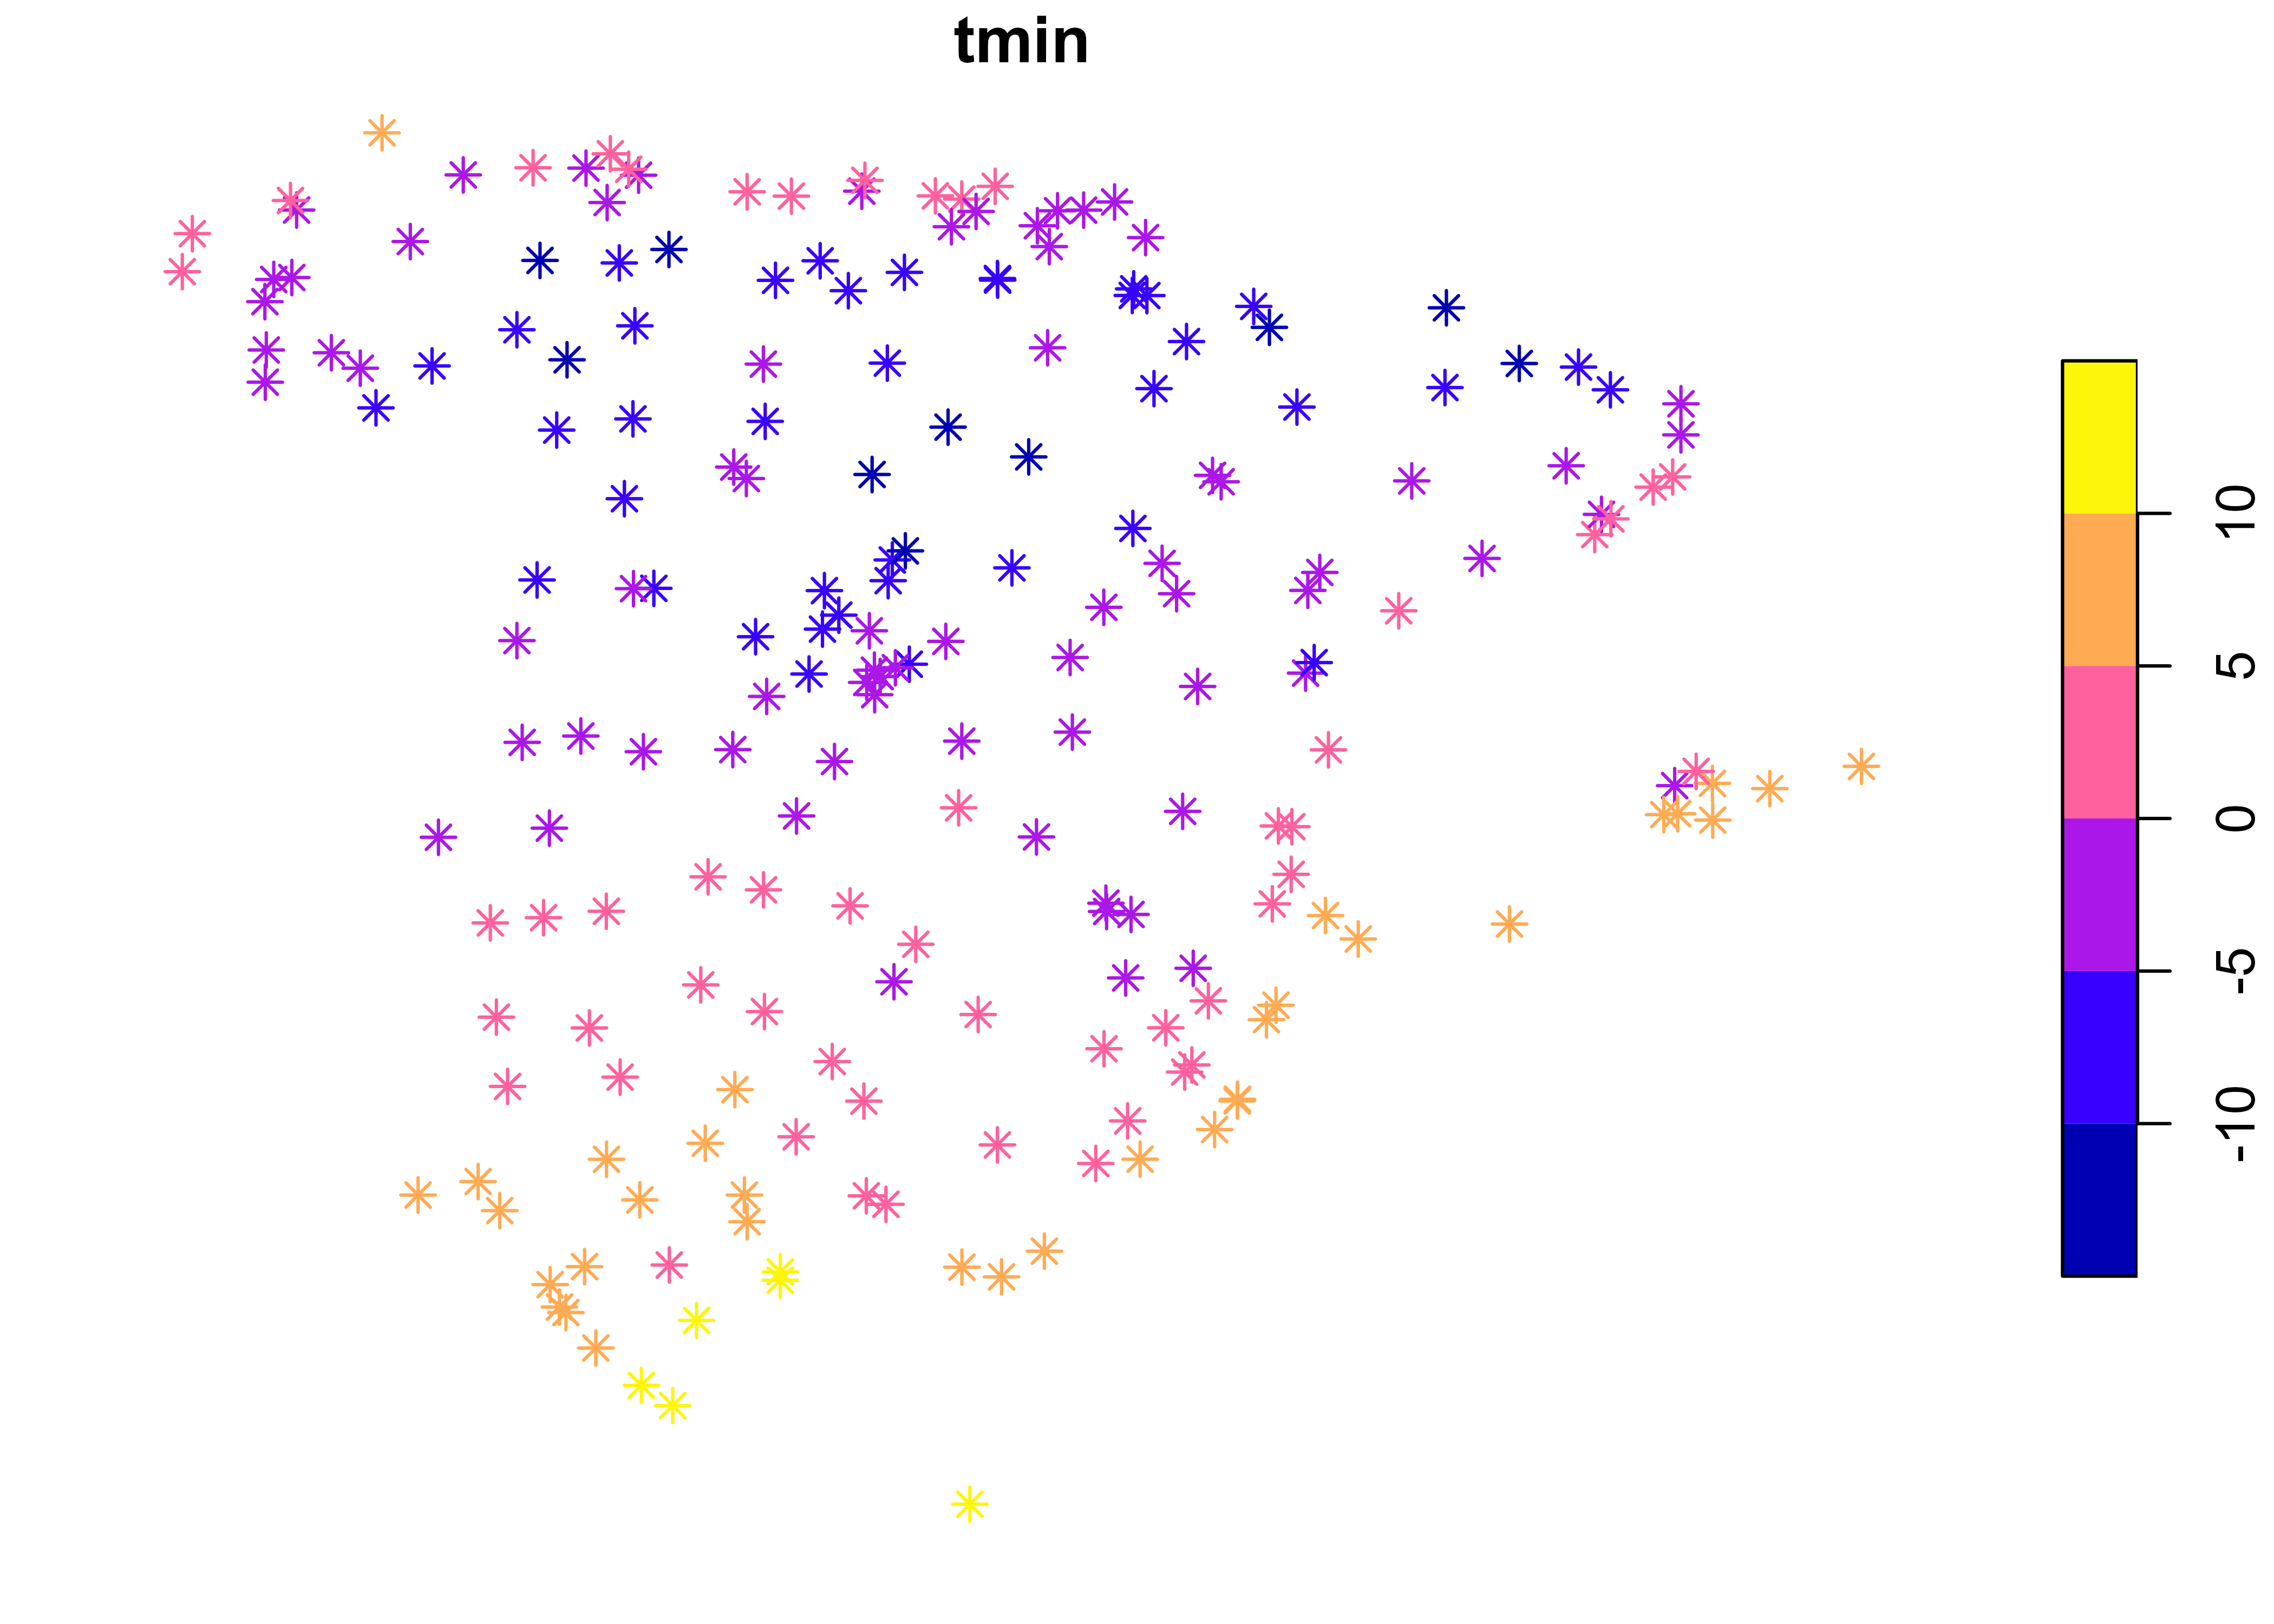
\includegraphics[width=0.6\linewidth]{_main_files/figure-latex/plot-base-tmin-1} 

}

\caption{Mapa de puntos con temperatura mínima (8-enero-2021)}\label{fig:plot-base-tmin}
\end{figure}

El mapa ha quedado muy bien, pero quizá los colores y el formato elegido no sean los más
adecuados para este tipo de representaciones\ldots{}

\begin{exercise}[plot-sp2]
\protect\hypertarget{exr:ex10}{}\label{exr:ex10}Utilice los parámetros espaciales de los que dispone, las coordenadas y
el contorno de España para graficar y contar la historia de \textbf{Filomena}
adecuadamente.
\end{exercise}

\begin{figure}

{\centering 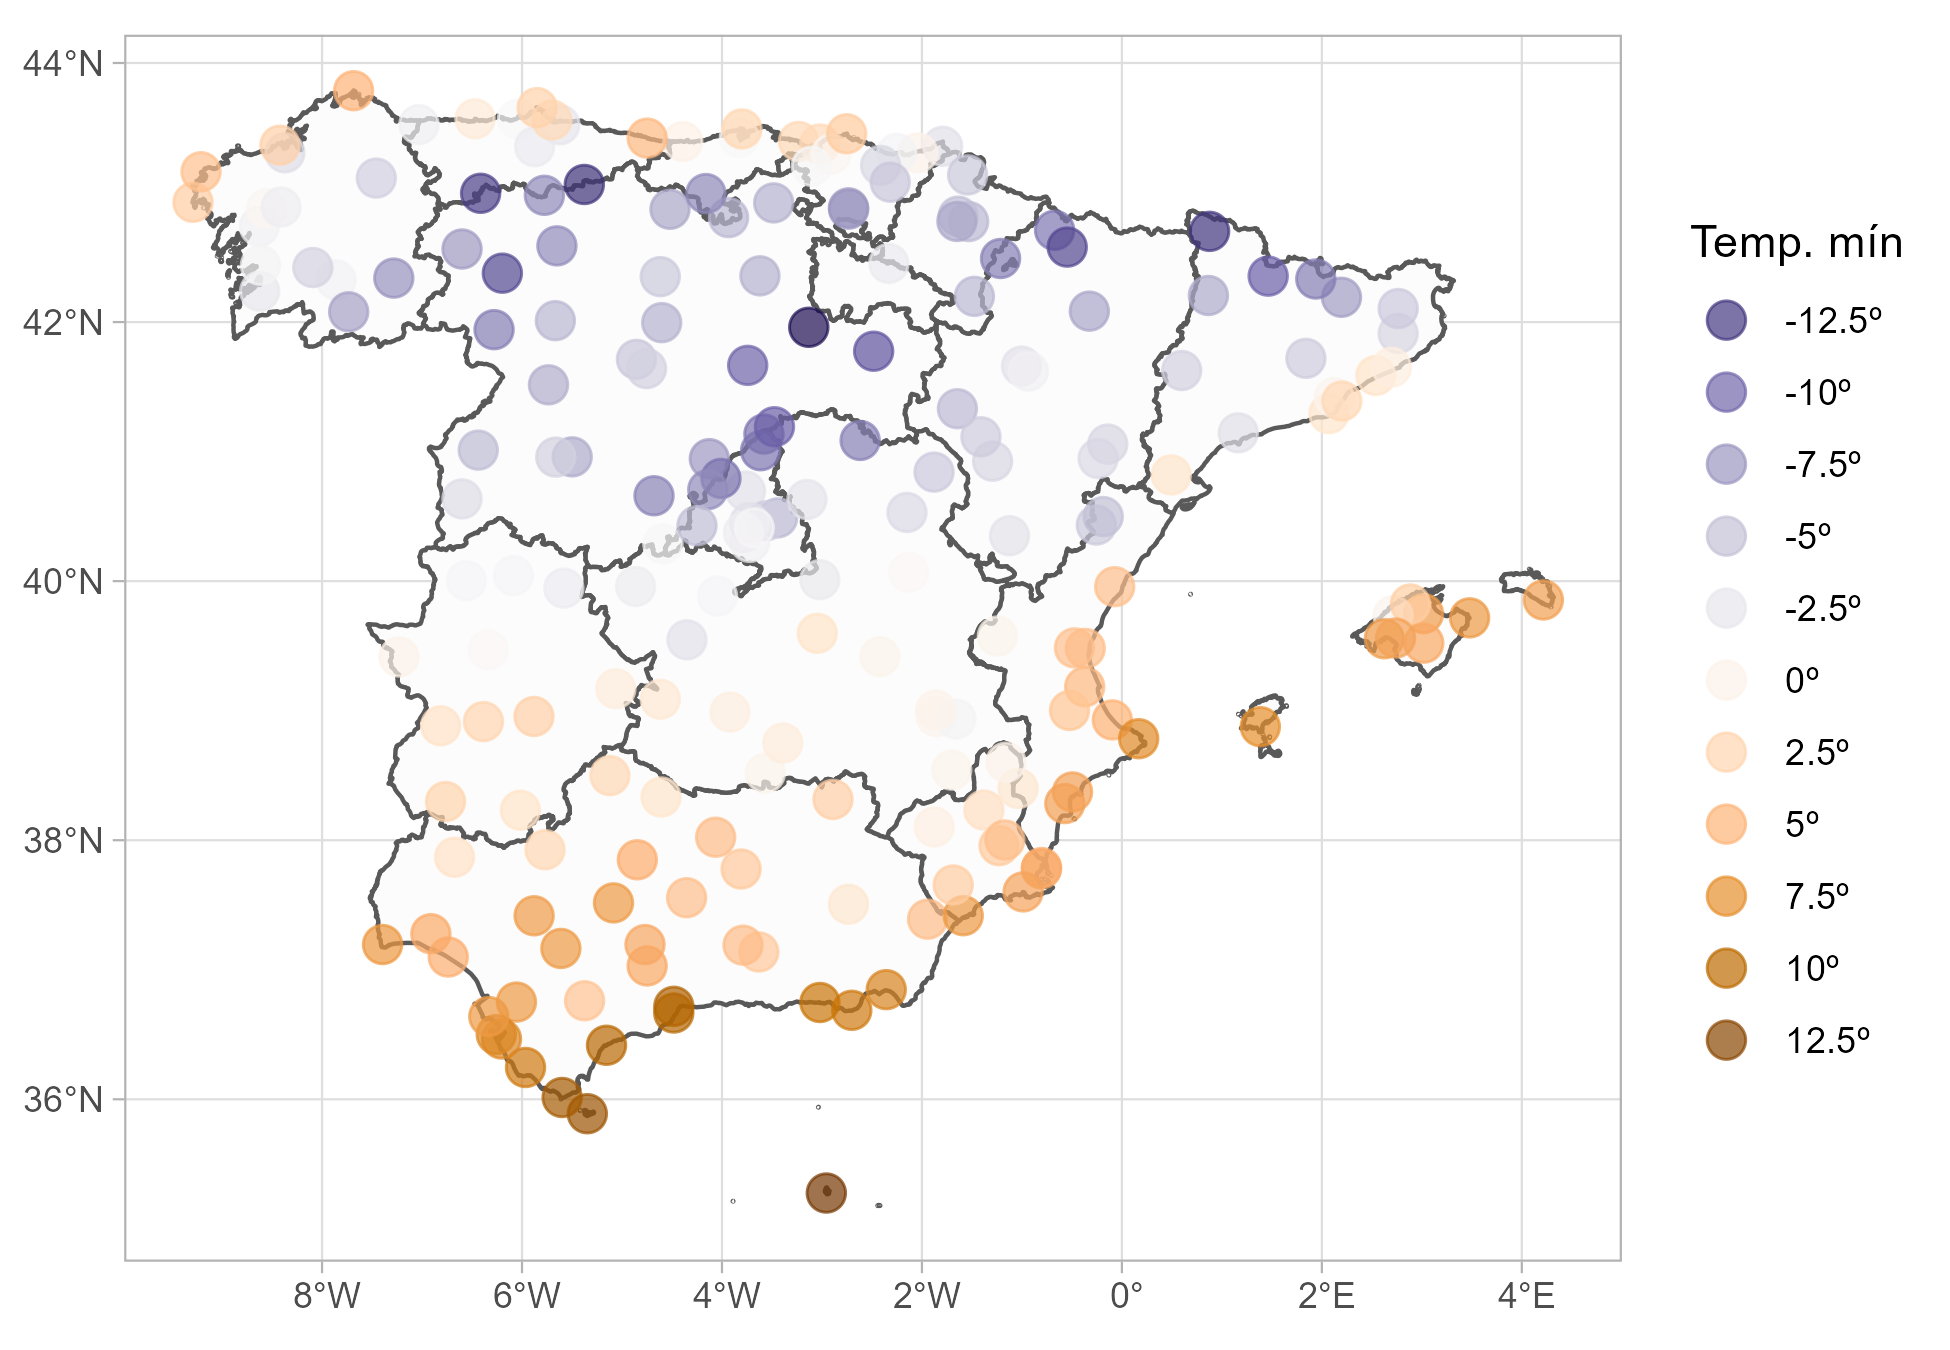
\includegraphics[width=0.6\linewidth]{_main_files/figure-latex/spatial-plots-1} 

}

\caption{Mapa completo con temperatura mínima (8-enero-2021)}\label{fig:spatial-plots}
\end{figure}

La visión que ofrece el la Fig. @ref\{fig:spatial-plots\} de Filomena es muy
informativa, vemos como los datos nos cuentan la historia de lo que ocurrió
ese día. La pena es que no existan estaciones de monitorero en todos los
puntos de España para conocer el valor de la temperatura mínima en cualquier
lugar del país. ¿Podríamos tener un mapa de interpolación para tener una estimación de la
temperatura mínima en las partes donde la AEMET no tiene estación de
monitoreo?

Tal y como se avanzó en el Capítulo \ref{dep-esp}, parece lógico pensar
que aquellos puntos que estén cerca tendrán valores similares. Por tanto,
tomemos ventaja de las propiedades de la dependencia
espacial y utilicemos un método de interpolación sencillo, en este caso
un método determinista, la Distancia Inversa
Ponderada, comúnmente conocido por su acrónimo inglés IDW (Inverse distance
weighted), el cual es uno de los métodos más simples para llevar para llevar a
cabo una interpolación espacial.

En este tipo de análisis espacial, es crucial que el CRS sea el apropiado. En este caso,
ya se definió el CRS como un CRS geográfico (es decir, usando coordenadas de
longitud y latitud). Sin embargo, para el ejercicio de interpolación es más
adecuado usar un CRS local (que provoca pocas deformaciones en la proyección de
España) y en alguna unidad de distancia, como metros (ya se vio en la Sección
XXXX que en los CRS geográficos las unidades son grados).

\begin{exercise}[Obtención de CRS sugerido para un conjuto de datos]
\protect\hypertarget{exr:ex11}{}\label{exr:ex11}Utilice el paquete \texttt{crsuggest} para observar los CRS sugeridos y, si es necesario,
transforme la proyección de los datos.
\end{exercise}

\begin{Shaded}
\begin{Highlighting}[]
\FunctionTok{library}\NormalTok{(crsuggest)}

\NormalTok{sugiere }\OtherTok{\textless{}{-}} \FunctionTok{suggest\_crs}\NormalTok{(tmin\_8enero, }\AttributeTok{units =} \StringTok{"m"}\NormalTok{, }\AttributeTok{limit =} \DecValTok{5}\NormalTok{)}

\CommentTok{\# Usamos la sugerencia del paquete}
\NormalTok{crs\_sugerido }\OtherTok{\textless{}{-}} \FunctionTok{st\_crs}\NormalTok{(sugiere[}\DecValTok{1}\NormalTok{, ]}\SpecialCharTok{$}\NormalTok{crs\_proj4) }\CommentTok{\# Madrid}

\NormalTok{esp3 }\OtherTok{\textless{}{-}} \FunctionTok{st\_transform}\NormalTok{(esp2, crs\_sugerido)}
\NormalTok{tmin\_8enero3 }\OtherTok{\textless{}{-}} \FunctionTok{st\_transform}\NormalTok{(tmin\_8enero, crs\_sugerido)}
\end{Highlighting}
\end{Shaded}

Una vez solucionado el problema de las proyecciones, antes de llevar a cabo la
interpolación, es necesario generar una malla que representará
las celdas de las que queremos obtener el valor interpolado.
Dado que hemos proyectado nuestros datos a un CRS cuya unidad son los metros,
podemos definir el tamaño de cada celda en metros cuadrados. En este caso vamos
a usar celdas de 100 kms cuadrados (10 x 10 kms).

\begin{exercise}[Creación y representación de una malla de interpolación]
\protect\hypertarget{exr:ex12}{}\label{exr:ex12}Genere un grid y llámelo \texttt{malla\_sf} (puede fijar una semilla si lo desea) y
grafíque la superficie construida.
\end{exercise}

\begin{Shaded}
\begin{Highlighting}[]

\CommentTok{\# Generación de la superficie a interpolar}
\FunctionTok{set.seed}\NormalTok{(}\DecValTok{9876}\NormalTok{) }\CommentTok{\# Aseguramos que el grid generado siempre es igual}

\NormalTok{malla\_sf }\OtherTok{\textless{}{-}} \FunctionTok{st\_make\_grid}\NormalTok{(}
\NormalTok{  esp3,}
  \AttributeTok{cellsize =} \DecValTok{8000}
\NormalTok{)}

\CommentTok{\# Representación de la superficie construida añadiendo el contorno de España}
\FunctionTok{ggplot}\NormalTok{(esp3) }\SpecialCharTok{+}
  \FunctionTok{geom\_sf}\NormalTok{() }\SpecialCharTok{+}
  \FunctionTok{geom\_sf}\NormalTok{(}
    \AttributeTok{data =}\NormalTok{ malla\_sf,}
    \AttributeTok{size =} \FloatTok{0.1}\NormalTok{,}
    \AttributeTok{col =} \StringTok{"red"}\NormalTok{, }\AttributeTok{alpha =} \DecValTok{1}\NormalTok{,}
    \AttributeTok{fill =} \ConstantTok{NA}
\NormalTok{  ) }\SpecialCharTok{+}
  \FunctionTok{geom\_sf}\NormalTok{(}
    \AttributeTok{data =}\NormalTok{ tmin\_8enero3,}
    \FunctionTok{aes}\NormalTok{(}\AttributeTok{fill =} \StringTok{"AEMET Stations"}\NormalTok{), }\AttributeTok{size =} \DecValTok{4}\NormalTok{, }\AttributeTok{shape =} \DecValTok{21}\NormalTok{,}
    \AttributeTok{color =} \StringTok{"blue"}
\NormalTok{  ) }\SpecialCharTok{+}
  \FunctionTok{scale\_fill\_manual}\NormalTok{(}\AttributeTok{values =} \FunctionTok{adjustcolor}\NormalTok{(}\StringTok{"blue"}\NormalTok{, }\AttributeTok{alpha.f =} \FloatTok{0.2}\NormalTok{)) }\SpecialCharTok{+}
  \FunctionTok{theme\_void}\NormalTok{() }\SpecialCharTok{+}
  \FunctionTok{theme}\NormalTok{(}\AttributeTok{legend.position =} \StringTok{"bottom"}\NormalTok{)}
\end{Highlighting}
\end{Shaded}

\begin{figure}

{\centering 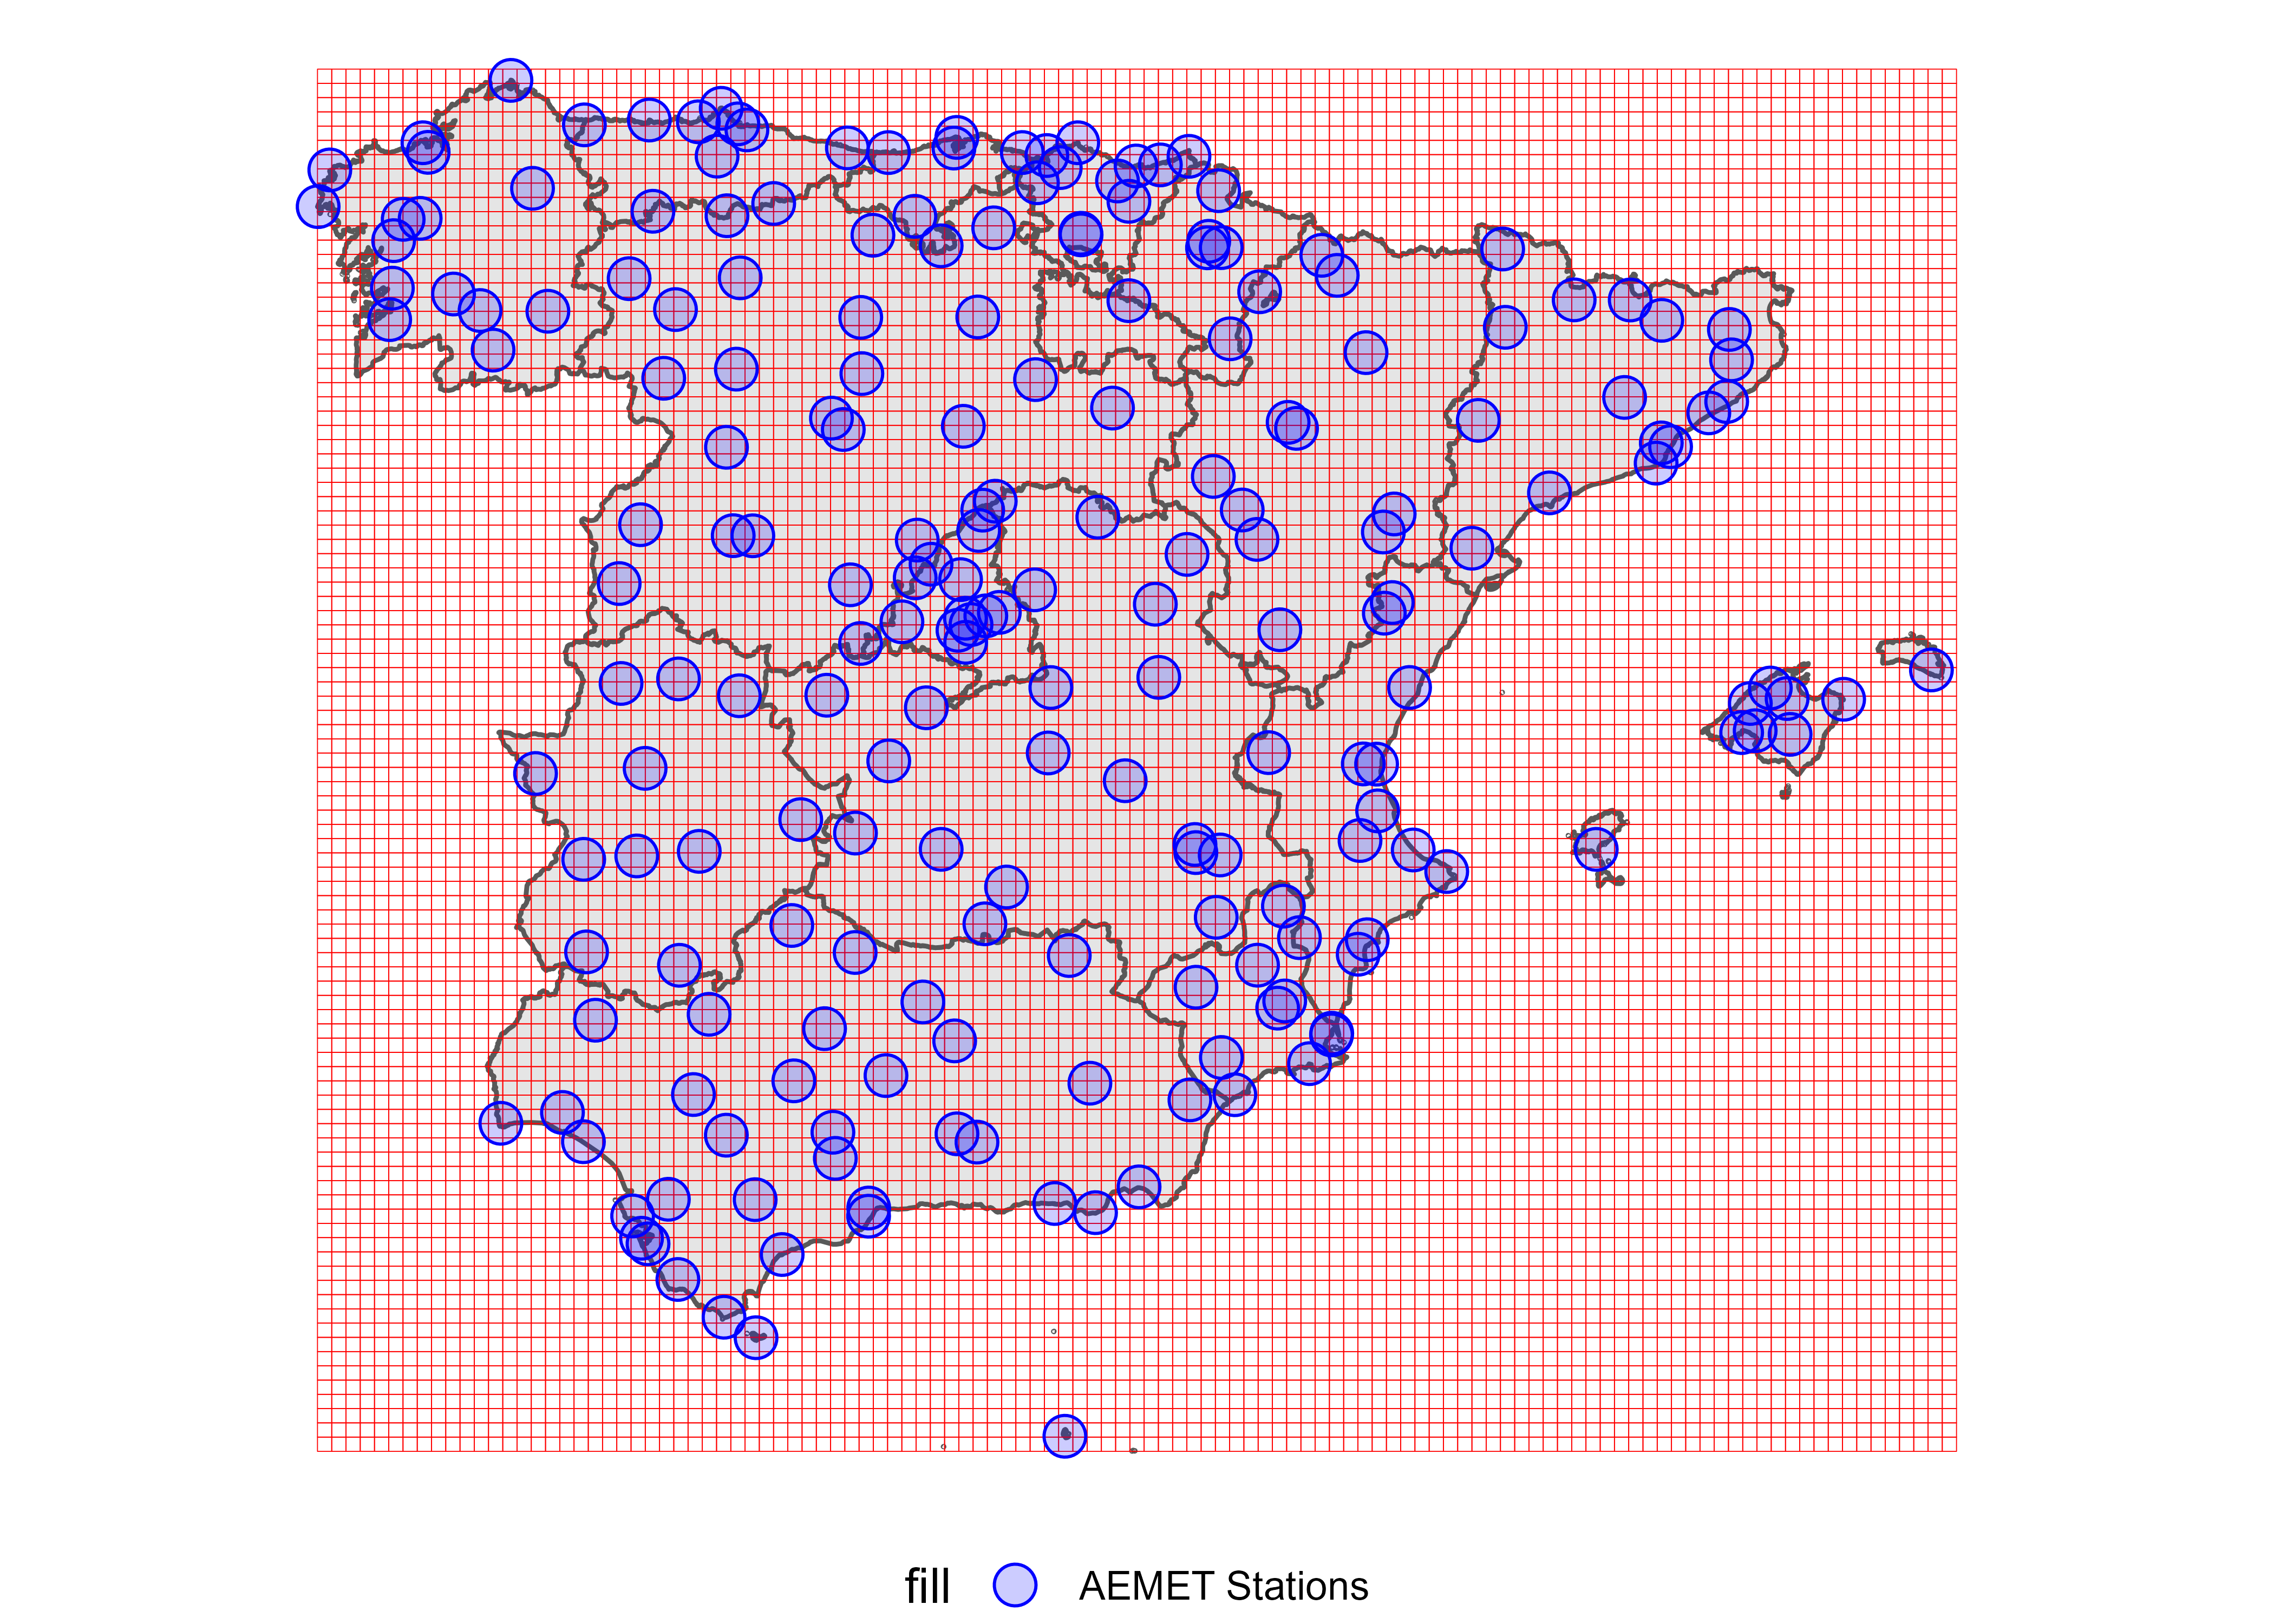
\includegraphics[width=0.6\linewidth]{_main_files/figure-latex/create-grid2-1} 

}

\caption{Malla de puntos para interpolación}\label{fig:create-grid2}
\end{figure}

Se puede observar claramente cada una de las celdas que se han creado. La
interpolación asignará un valor a cada uno de ellas.

A continuación podemos llevar a cabo la interpolación usando el paquete \texttt{gstat}.
Además, en lugar de celdas (polígonos) es necesario usar puntos en la
interpolación. Calcularemos, por tanto, un punto representativo de cada celda
creada en la superficie anterior \texttt{malla\_sf}, el centroide,
que es el punto resultante de realizar la media arimética de las
coordenadas de los puntos que componen los lados de cada celda.

\begin{exercise}[Interpolación a través de la Distancia Inversa Ponderada]
\protect\hypertarget{exr:ex13}{}\label{exr:ex13}Calcule los centroides de los polígonos de la malla construida
en el Ejercicio \ref{exr:ex12} con la función \texttt{st\_centroide}
y realice una interpolación de la variable temperatura mínima
\texttt{tmin} para el día 8 de enero de 2021 con el método IDW usando la librería
\texttt{gstat} y la función \texttt{idw}. Guarde el resultado obtenido en un objeto llamado
\texttt{tmin\_idw}. Utilice la función \texttt{help(idw)} si requiere
información sobre cómo introducir los parámetros en la función.

Examine la información del objeto \texttt{tmin\_idw}, a través de la función \texttt{head},
\end{exercise}

\begin{Shaded}
\begin{Highlighting}[]
\CommentTok{\# Calculamos una malla con centroides}
\NormalTok{malla\_sf\_cent }\OtherTok{\textless{}{-}} \FunctionTok{st\_centroid}\NormalTok{(malla\_sf, }\AttributeTok{of\_largest\_polygon =} \ConstantTok{TRUE}\NormalTok{)}

\FunctionTok{library}\NormalTok{(gstat)}
\NormalTok{tmin\_idw }\OtherTok{\textless{}{-}} \FunctionTok{idw}\NormalTok{(}
  \CommentTok{\# Indicamos la variable que queremos interpolar}
\NormalTok{  tmin }\SpecialCharTok{\textasciitilde{}} \DecValTok{1}\NormalTok{,}
  \CommentTok{\# Indicamos el conjunto de datos donde está la variable}
\NormalTok{  tmin\_8enero3,}
  \CommentTok{\# Indicamos la malla de destino, en sf}
  \AttributeTok{newdata =}\NormalTok{ malla\_sf\_cent,}
  \AttributeTok{idp =} \FloatTok{2.0} \CommentTok{\# Especifica la potencia de la IDW}
\NormalTok{)}
\CommentTok{\#\textgreater{} [inverse distance weighted interpolation]}
\FunctionTok{head}\NormalTok{(tmin\_idw)}
\CommentTok{\#\textgreater{} Simple feature collection with 6 features and 2 fields}
\CommentTok{\#\textgreater{} Geometry type: POINT}
\CommentTok{\#\textgreater{} Dimension:     XY}
\CommentTok{\#\textgreater{} Bounding box:  xmin: 146290.9 ymin: 69457.31 xmax: 186290.9 ymax: 69457.31}
\CommentTok{\#\textgreater{} CRS:           +proj=lcc +lat\_1=40 +lat\_0=40 +lon\_0=0 +k\_0=0.9988085293 +x\_0=600000 +y\_0=600000 +a=6378298.3 +rf=294.73 +pm=madrid +units=m +no\_defs}
\CommentTok{\#\textgreater{}   var1.pred var1.var                  geometry}
\CommentTok{\#\textgreater{} 1  2.518621       NA POINT (146290.9 69457.31)}
\CommentTok{\#\textgreater{} 2  2.586930       NA POINT (154290.9 69457.31)}
\CommentTok{\#\textgreater{} 3  2.656846       NA POINT (162290.9 69457.31)}
\CommentTok{\#\textgreater{} 4  2.728395       NA POINT (170290.9 69457.31)}
\CommentTok{\#\textgreater{} 5  2.801600       NA POINT (178290.9 69457.31)}
\CommentTok{\#\textgreater{} 6  2.876486       NA POINT (186290.9 69457.31)}
\end{Highlighting}
\end{Shaded}

Un tipo de mapas muy utilizado cuando se trabaja con datos espaciales son los
mapas de contorno. Es muy visual y ayuda a interpretar el mapa interpolado,
añadir unas lineas de contorno al mapa interpolado.

\begin{exercise}[Mapa de interpolación y contorno con `raster`]
\protect\hypertarget{exr:ex14}{}\label{exr:ex14}Represente los valores interpolados, \texttt{tmin\_idw}, y añada unas lineas de contorno.
Utilice el paquete \texttt{raster} para convertir el objeto interpolado a pixeles.
\end{exercise}

\begin{Shaded}
\begin{Highlighting}[]
\CommentTok{\# Convertimos de sf a SpatiaPixels}
\CommentTok{\# Esto funciona porque nuestros puntos sf están espaciados regularmente}

\NormalTok{tmin\_pixels }\OtherTok{\textless{}{-}}\NormalTok{ tmin\_idw }\SpecialCharTok{\%\textgreater{}\%}
  \FunctionTok{as}\NormalTok{(}\StringTok{"Spatial"}\NormalTok{) }\SpecialCharTok{\%\textgreater{}\%}
  \FunctionTok{as}\NormalTok{(}\StringTok{"SpatialPixels"}\NormalTok{)}


\FunctionTok{library}\NormalTok{(raster)}
\CommentTok{\# Creamos un raster de nuestros pixels}
\NormalTok{rast\_esp }\OtherTok{\textless{}{-}} \FunctionTok{raster}\NormalTok{(tmin\_pixels)}

\CommentTok{\# Transferimos valores del objeto sf al raster}
\NormalTok{rast\_esp2 }\OtherTok{\textless{}{-}} \FunctionTok{rasterize}\NormalTok{(}
\NormalTok{  tmin\_idw,}
\NormalTok{  rast\_esp,}
  \AttributeTok{field =} \StringTok{"var1.pred"}\NormalTok{, }\DocumentationTok{\#\# valores de predicción idw}
  \AttributeTok{fun =}\NormalTok{ mean}
\NormalTok{)}

\CommentTok{\# Además, podemos recortar el raster a la forma de España}

\NormalTok{rast\_esp\_mask }\OtherTok{\textless{}{-}} \FunctionTok{mask}\NormalTok{(rast\_esp2, esp3)}

\FunctionTok{plot}\NormalTok{(rast\_esp\_mask, }\AttributeTok{col =}\NormalTok{ colores)}
\FunctionTok{contour}\NormalTok{(rast\_esp2, }\AttributeTok{add =} \ConstantTok{TRUE}\NormalTok{)}
\end{Highlighting}
\end{Shaded}

\begin{figure}

{\centering 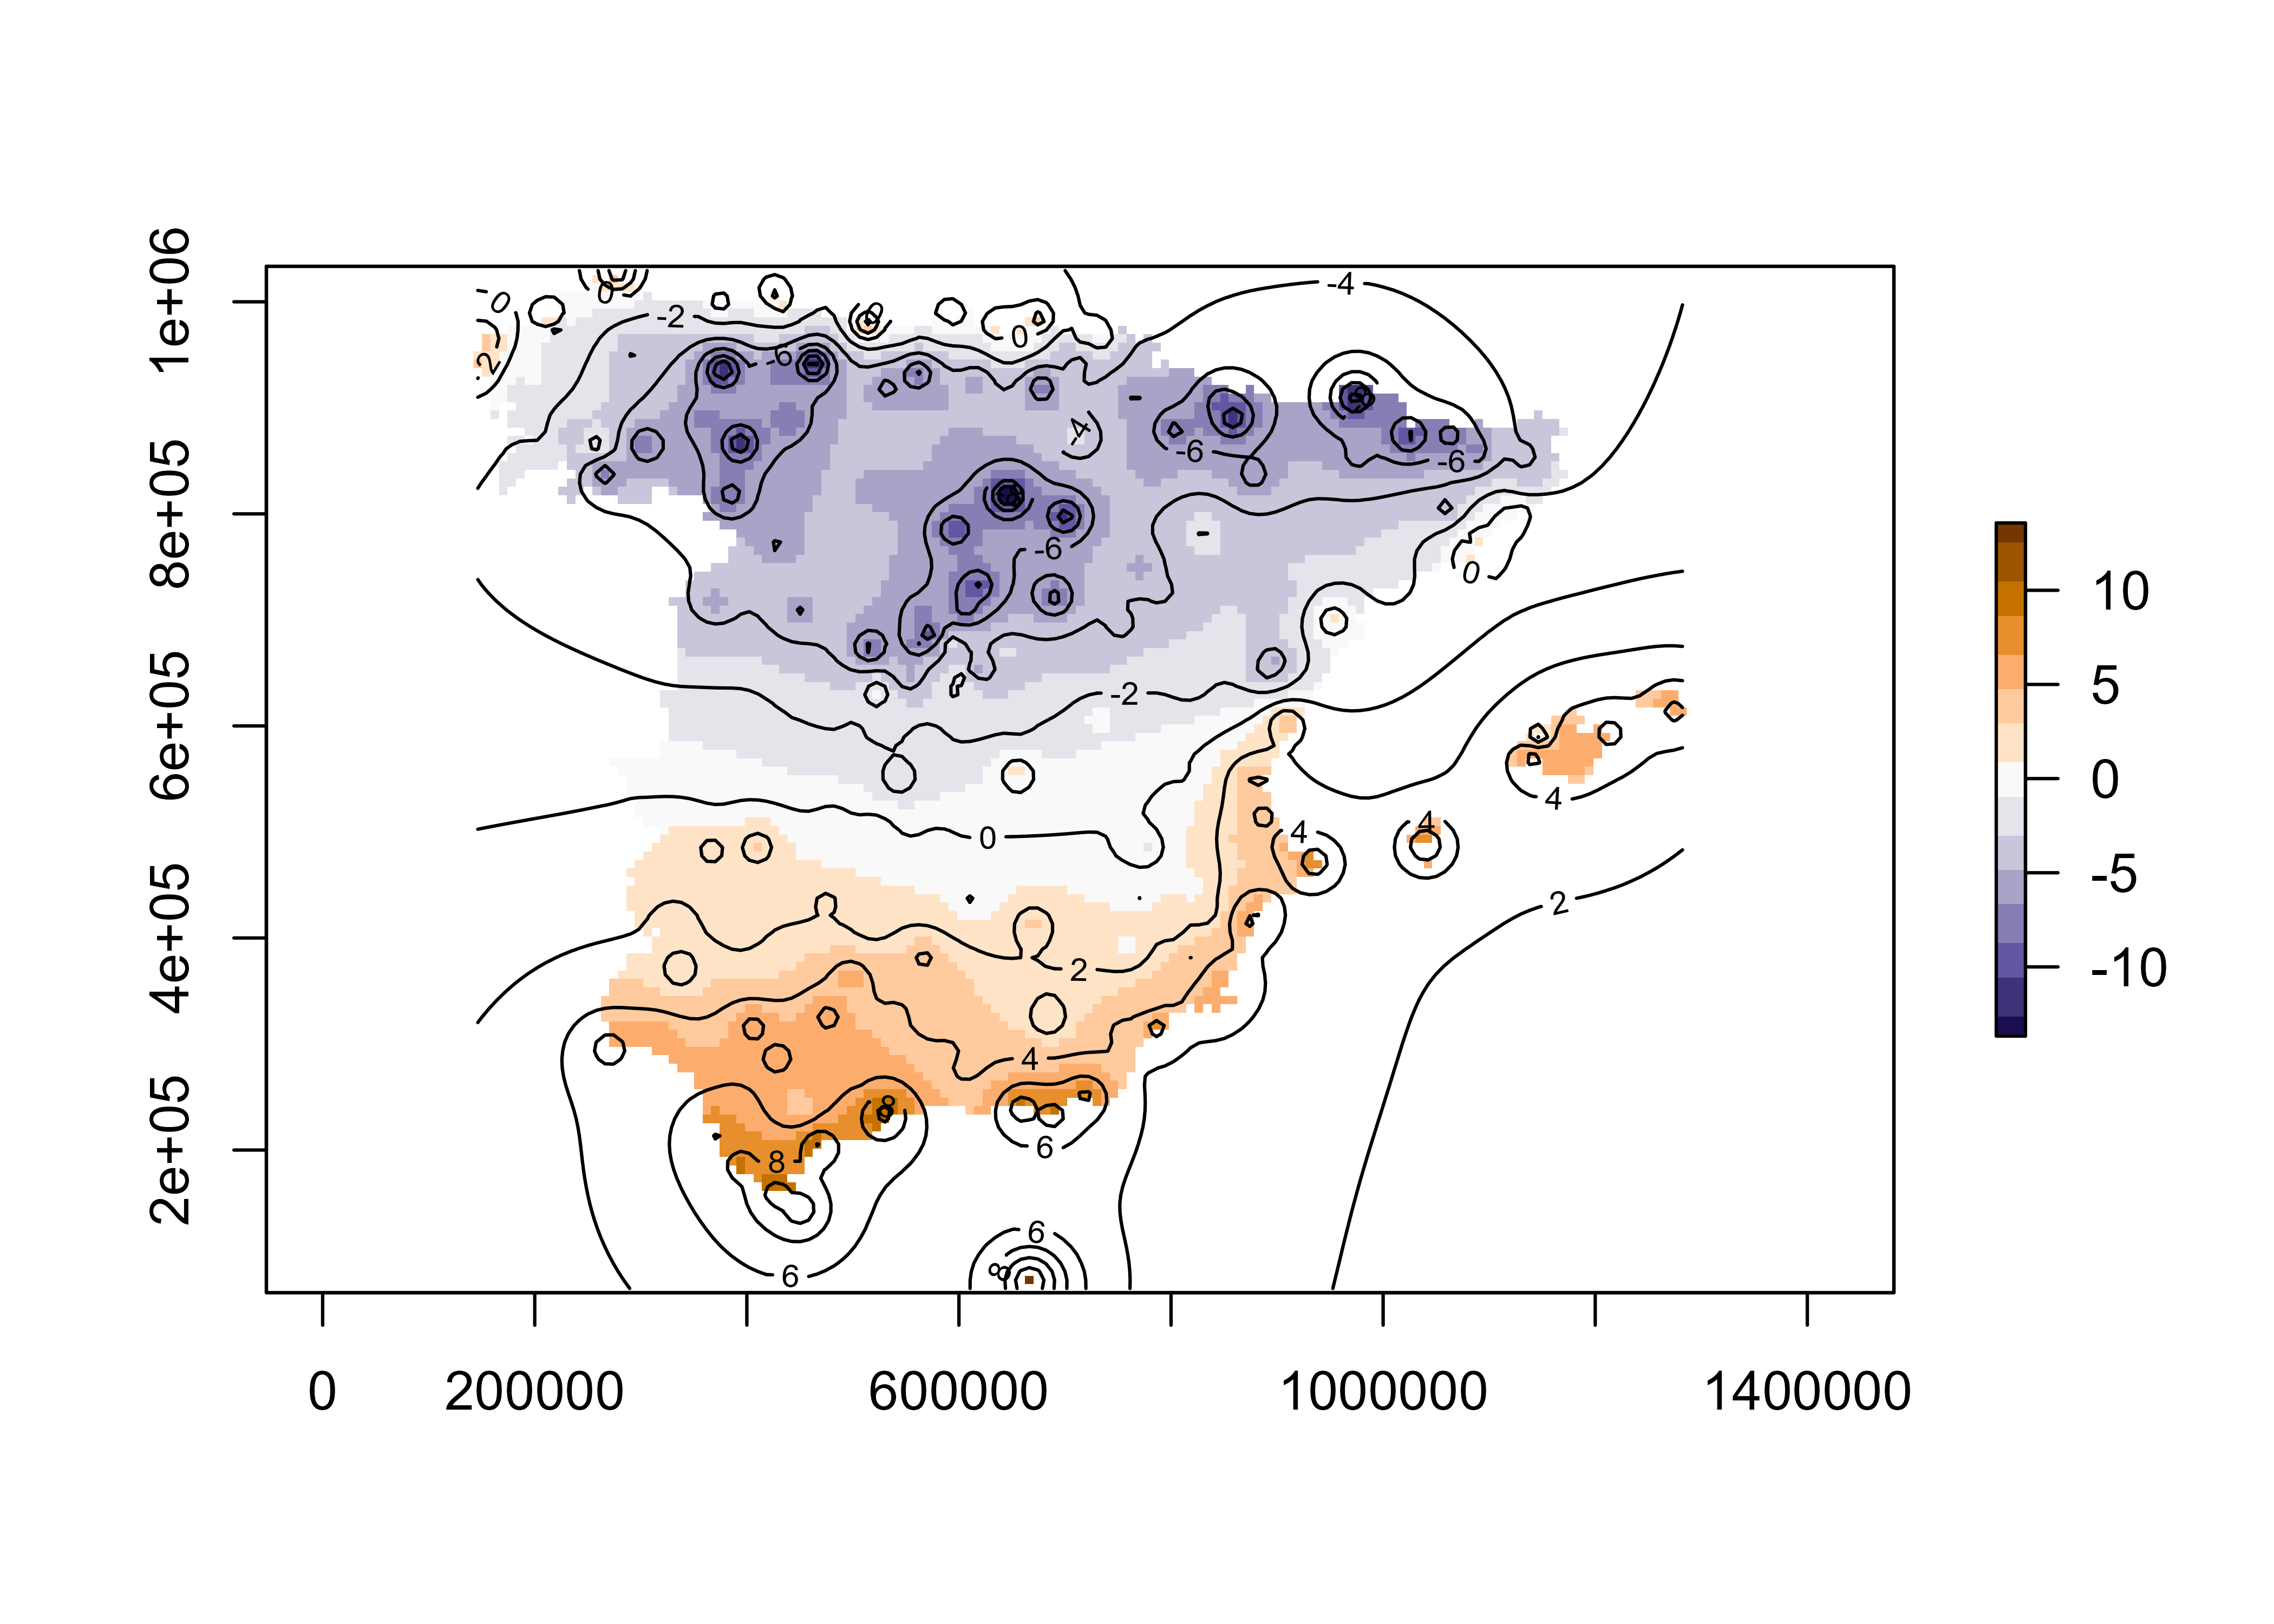
\includegraphics[width=0.6\linewidth]{_main_files/figure-latex/unnamed-chunk-16-1} 

}

\caption{Mapa raster con lineas de nivel}\label{fig:unnamed-chunk-16}
\end{figure}

\begin{exercise}[Mapa de interpolación con `ggplot`]
\protect\hypertarget{exr:ex15}{}\label{exr:ex15}Repita el mapa de \ref{exr:ex14} usando \texttt{ggplot2} y la función
\texttt{geom\_contour\_filled}.
\end{exercise}

\begin{Shaded}
\begin{Highlighting}[]

\CommentTok{\# Creo una tabla para geom contour}
\NormalTok{coordenadas }\OtherTok{\textless{}{-}} \FunctionTok{st\_coordinates}\NormalTok{(tmin\_idw)}
\NormalTok{valor }\OtherTok{\textless{}{-}}\NormalTok{ tmin\_idw}\SpecialCharTok{$}\NormalTok{var1.pred}

\NormalTok{idw\_df }\OtherTok{\textless{}{-}} \FunctionTok{data.frame}\NormalTok{(}
  \CommentTok{\# Necesitamos redondear las coordenadas}
  \AttributeTok{latitud =} \FunctionTok{round}\NormalTok{(coordenadas[, }\DecValTok{2}\NormalTok{], }\DecValTok{6}\NormalTok{),}
  \AttributeTok{longitud =} \FunctionTok{round}\NormalTok{(coordenadas[, }\DecValTok{1}\NormalTok{], }\DecValTok{6}\NormalTok{),}
  \AttributeTok{tmin =}\NormalTok{ valor}
\NormalTok{)}

\FunctionTok{ggplot}\NormalTok{() }\SpecialCharTok{+}
  \FunctionTok{geom\_contour\_filled}\NormalTok{(}
    \AttributeTok{data =}\NormalTok{ idw\_df,}
    \FunctionTok{aes}\NormalTok{(}\AttributeTok{x =}\NormalTok{ longitud, }\AttributeTok{y =}\NormalTok{ latitud, }\AttributeTok{z =}\NormalTok{ tmin),}
    \AttributeTok{na.rm =} \ConstantTok{TRUE}\NormalTok{,}
    \AttributeTok{breaks =}\NormalTok{ cortes}
\NormalTok{  ) }\SpecialCharTok{+}
  \CommentTok{\# Reajustamos la escala de colores}
  \FunctionTok{scale\_fill\_manual}\NormalTok{(}\AttributeTok{values =}\NormalTok{ colores) }\SpecialCharTok{+}
  \CommentTok{\# CCAA}
  \FunctionTok{geom\_sf}\NormalTok{(}\AttributeTok{data =}\NormalTok{ esp3, }\AttributeTok{fill =} \ConstantTok{NA}\NormalTok{) }\SpecialCharTok{+}
  \FunctionTok{theme\_minimal}\NormalTok{() }\SpecialCharTok{+}
  \FunctionTok{theme}\NormalTok{(}\AttributeTok{axis.title =} \FunctionTok{element\_blank}\NormalTok{()) }\SpecialCharTok{+}
  \FunctionTok{labs}\NormalTok{(}
    \AttributeTok{fill =} \StringTok{"Temp. (º)"}\NormalTok{,}
    \CommentTok{\#  title = "Temperatura mínima interpolada",}
    \CommentTok{\#  subtitle = "8 de Enero 2021",}
    \CommentTok{\#  caption = "Datos: AEMET"}
\NormalTok{  )}
\end{Highlighting}
\end{Shaded}

\begin{figure}

{\centering 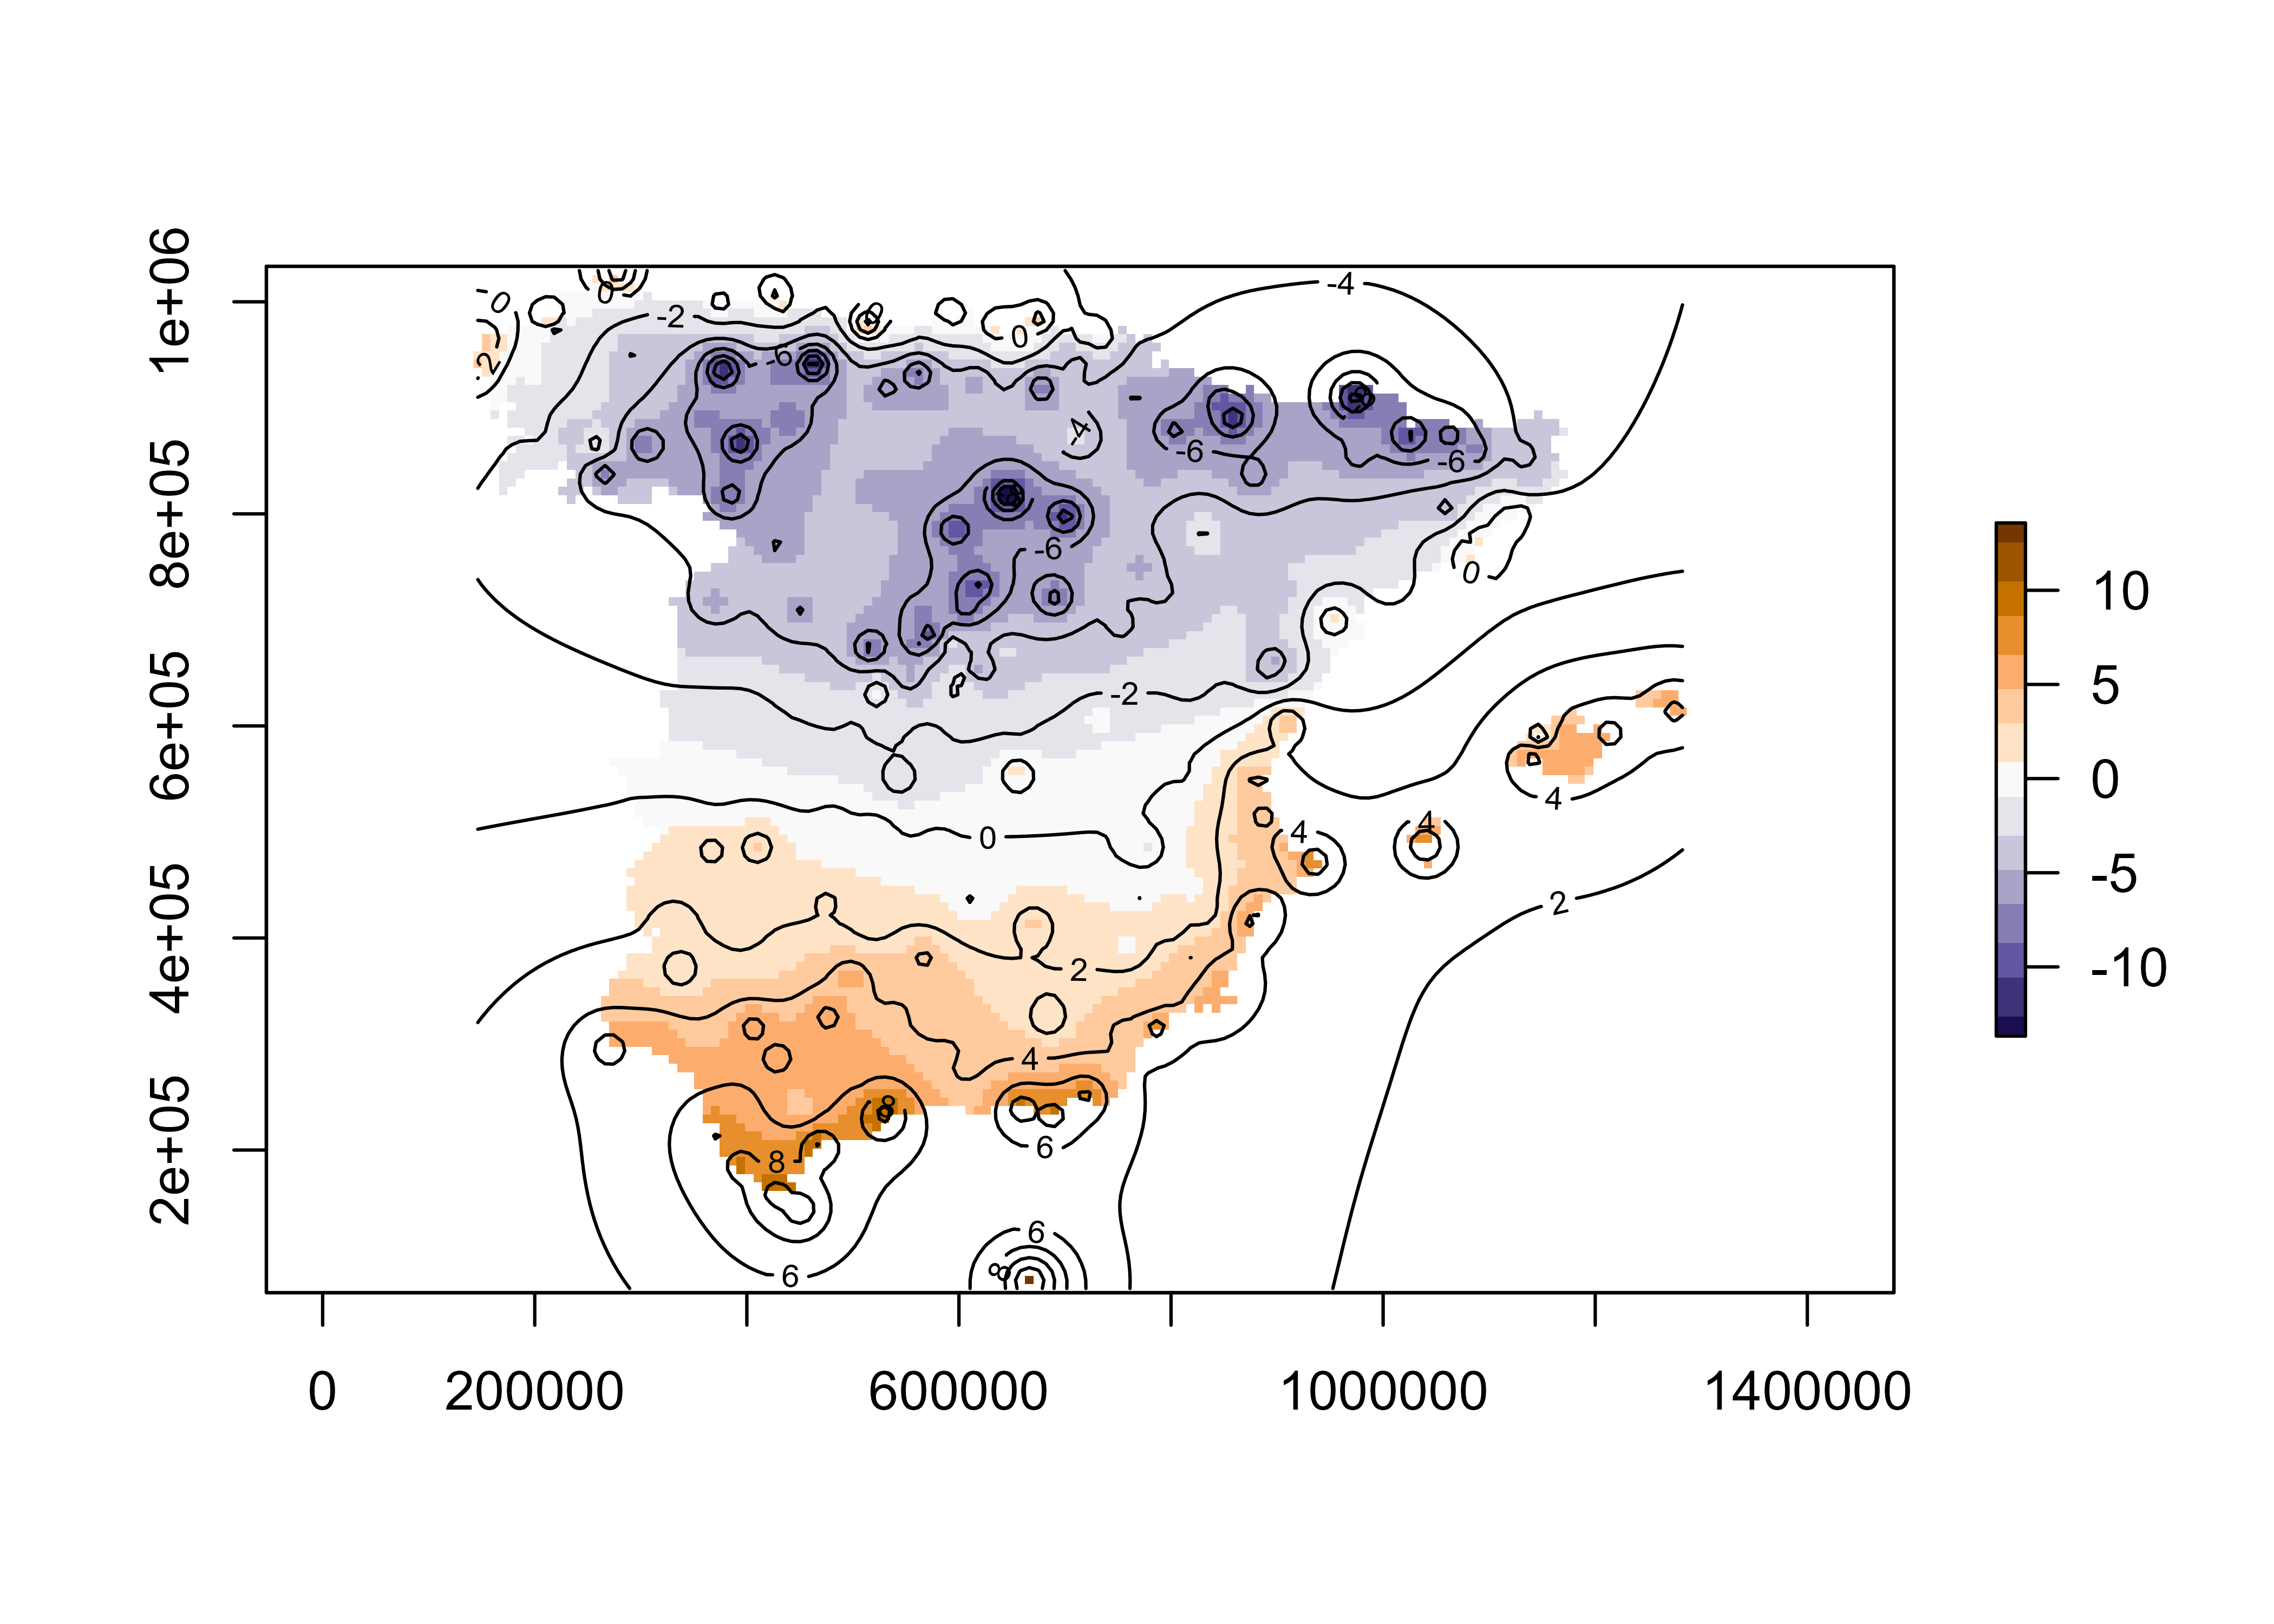
\includegraphics[width=0.6\linewidth]{_main_files/figure-latex/unnamed-chunk-17-1} 

}

\caption{Temperatura mínima interpolada. 8 de Enero 2021. }\label{fig:unnamed-chunk-17}
\end{figure}

\hypertarget{caso-2.-distribuciuxf3n-espacial-de-la-renta-media-por-municipios}{%
\section{Caso 2. Distribución espacial de la renta media por municipios}\label{caso-2.-distribuciuxf3n-espacial-de-la-renta-media-por-municipios}}

** Objetivos de aprendizaje **

Esta sección presenta un caso de uso en el que aprenderemos a realizar las
siguientes tareas básicas:

\begin{itemize}
\item
  Importar datos tabulares y datos espaciales.
\item
  Realizar un tratamiento de limpieza de datos y cruzar tablas.
\item
  Hacer mapas temáticos. Aprenderemos también algunas nociones básicas sobre
  cómo crear diferentes clases para un conjunto de datos continuo.
\end{itemize}

Para ello, partiremos de dos ficheros:

\begin{enumerate}
\def\labelenumi{\arabic{enumi}.}
\item
  Fichero \texttt{renta\_municipio.csv}: Este fichero contiene información de la Renta
  Neta per cápita por municipios (en euros), distritos y secciones censales.
  Esta información se ha extraído del \href{https://www.ine.es/experimental/atlas/experimental_atlas.htm}{Atlas de distribución de renta de los
  hogares}
  proporcionado por el INE, y ha sido tratado previamente para adaptar la
  información al presente ejercicio.
\item
  Fichero \texttt{municipios.gpkg}: Es un fichero que contiene datos espaciales
  (polígonos) de los municipios en España en el año 2019. Se ha extraído del
  Instituto Geográfico Nacional (IGN) usando el paquete \texttt{mapSpain}.
\end{enumerate}

El primer paso en cualquier tipo de análisis de datos es importar los datos al
software de tratamiento (en nuestro caso, R) y analizarlos para conocer el tipo
de información que contiene.

\begin{exercise}[Importación y análisis del los datos objeto de estudio]
\protect\hypertarget{exr:ex16}{}\label{exr:ex16}Importe el fichero de datos \texttt{renta\_municipio.csv} y \texttt{municipios.gpkg}
y guárdelo en un objeto llamado \texttt{renta} y \texttt{munis}, respectivamente.
Observe la información que contienen. Puede ayudarse de la función \texttt{head.}
Use las librerías oportunas par iportar los datos en los distintos formatos.
\end{exercise}

\begin{Shaded}
\begin{Highlighting}[]
\CommentTok{\# Usaremos paquetes del tidyverse}
\FunctionTok{library}\NormalTok{(dplyr)}
\FunctionTok{library}\NormalTok{(readr)}

\NormalTok{renta }\OtherTok{\textless{}{-}} \FunctionTok{read\_csv}\NormalTok{(}\StringTok{"data/renta\_municipio.csv"}\NormalTok{, }\AttributeTok{na =} \StringTok{"."}\NormalTok{)}
\end{Highlighting}
\end{Shaded}

\begin{Shaded}
\begin{Highlighting}[]
\FunctionTok{library}\NormalTok{(sf)}
\NormalTok{munis }\OtherTok{\textless{}{-}} \FunctionTok{st\_read}\NormalTok{(}\StringTok{"data/municipios.gpkg"}\NormalTok{, }\AttributeTok{quiet =} \ConstantTok{TRUE}\NormalTok{)}
\end{Highlighting}
\end{Shaded}

\begin{Shaded}
\begin{Highlighting}[]
\FunctionTok{head}\NormalTok{(renta)}
\CommentTok{\#\textgreater{} \# A tibble: 6 x 6}
\CommentTok{\#\textgreater{}   Unidad                          \textasciigrave{}2019\textasciigrave{} \textasciigrave{}2018\textasciigrave{} \textasciigrave{}2017\textasciigrave{} \textasciigrave{}2016\textasciigrave{} \textasciigrave{}2015\textasciigrave{}}
\CommentTok{\#\textgreater{}   \textless{}chr\textgreater{}                            \textless{}dbl\textgreater{}  \textless{}dbl\textgreater{}  \textless{}dbl\textgreater{}  \textless{}dbl\textgreater{}  \textless{}dbl\textgreater{}}
\CommentTok{\#\textgreater{} 1 44001 Ababuj                        NA     NA     NA     NA     NA}
\CommentTok{\#\textgreater{} 2 4400101 Ababuj distrito 01          NA     NA     NA     NA     NA}
\CommentTok{\#\textgreater{} 3 4400101001 Ababuj sección 01001     NA     NA     NA     NA     NA}
\CommentTok{\#\textgreater{} 4 40001 Abades                     11429  10731  10314   9816   9904}
\CommentTok{\#\textgreater{} 5 4000101 Abades distrito 01       11429  10731  10314   9816   9904}
\CommentTok{\#\textgreater{} 6 4000101001 Abades sección 01001  11429  10731  10314   9816   9904}
\end{Highlighting}
\end{Shaded}

Se puede comprobar que tenemos información para el periodo 2015-2019. Además, la
columna \texttt{Unidad} contiene un literal con el municipio o sección correspondiente.

\begin{Shaded}
\begin{Highlighting}[]
\FunctionTok{head}\NormalTok{(munis)}
\CommentTok{\#\textgreater{} Simple feature collection with 6 features and 7 fields}
\CommentTok{\#\textgreater{} Geometry type: MULTIPOLYGON}
\CommentTok{\#\textgreater{} Dimension:     XY}
\CommentTok{\#\textgreater{} Bounding box:  xmin: {-}3.140179 ymin: 36.73817 xmax: {-}2.057058 ymax: 37.54579}
\CommentTok{\#\textgreater{} Geodetic CRS:  ETRS89}
\CommentTok{\#\textgreater{}   codauto ine.ccaa.name cpro ine.prov.name cmun      name LAU\_CODE}
\CommentTok{\#\textgreater{} 1      01     Andalucía   04       Almería  001      Abla    04001}
\CommentTok{\#\textgreater{} 2      01     Andalucía   04       Almería  002  Abrucena    04002}
\CommentTok{\#\textgreater{} 3      01     Andalucía   04       Almería  003      Adra    04003}
\CommentTok{\#\textgreater{} 4      01     Andalucía   04       Almería  004 Albanchez    04004}
\CommentTok{\#\textgreater{} 5      01     Andalucía   04       Almería  005 Alboloduy    04005}
\CommentTok{\#\textgreater{} 6      01     Andalucía   04       Almería  006     Albox    04006}
\CommentTok{\#\textgreater{}                             geom}
\CommentTok{\#\textgreater{} 1 MULTIPOLYGON ((({-}2.775594 3...}
\CommentTok{\#\textgreater{} 2 MULTIPOLYGON ((({-}2.787566 3...}
\CommentTok{\#\textgreater{} 3 MULTIPOLYGON ((({-}3.051988 3...}
\CommentTok{\#\textgreater{} 4 MULTIPOLYGON ((({-}2.181086 3...}
\CommentTok{\#\textgreater{} 5 MULTIPOLYGON ((({-}2.572442 3...}
\CommentTok{\#\textgreater{} 6 MULTIPOLYGON ((({-}2.128106 3...}
\end{Highlighting}
\end{Shaded}

El objeto \texttt{munis} contiene Polígonos y varias
columnas, entre ellas dos especialmente relevantes: \texttt{cpro} y \texttt{cmun}, que
corresponden a los códigos de provincia y de municipio respectivamente. Podemos
comprobar que este código también se encuentra en el dataset \texttt{renta}.

\begin{exercise}[Comprobación de campos en común para un municipio: Noblejas]
\protect\hypertarget{exr:ex17}{}\label{exr:ex17}Para comrobar que efectivamente disponemos de dos campos en comun en los ficheros,
que serán de vital importancia para posteriormente unirlos, se selecciona un
municipio al azar, el municipio de Noblejas en la provincia de Toledo y
comprobamos.
\end{exercise}

\begin{Shaded}
\begin{Highlighting}[]
\CommentTok{\# Miro un municipio: Noblejas}

\NormalTok{renta[}\FunctionTok{grep}\NormalTok{(}\StringTok{"Noblejas"}\NormalTok{, renta}\SpecialCharTok{$}\NormalTok{Unidad), ]}
\CommentTok{\#\textgreater{} \# A tibble: 5 x 6}
\CommentTok{\#\textgreater{}   Unidad                            \textasciigrave{}2019\textasciigrave{} \textasciigrave{}2018\textasciigrave{} \textasciigrave{}2017\textasciigrave{} \textasciigrave{}2016\textasciigrave{} \textasciigrave{}2015\textasciigrave{}}
\CommentTok{\#\textgreater{}   \textless{}chr\textgreater{}                              \textless{}dbl\textgreater{}  \textless{}dbl\textgreater{}  \textless{}dbl\textgreater{}  \textless{}dbl\textgreater{}  \textless{}dbl\textgreater{}}
\CommentTok{\#\textgreater{} 1 45115 Noblejas                     10591  10314   9751   9484   9124}
\CommentTok{\#\textgreater{} 2 4511501 Noblejas distrito 01       11039  10717  10135   9711   9386}
\CommentTok{\#\textgreater{} 3 4511501001 Noblejas sección 01001  11039  10717  10135   9711   9386}
\CommentTok{\#\textgreater{} 4 4511502 Noblejas distrito 02       10276  10029   9475   9319   8938}
\CommentTok{\#\textgreater{} 5 4511502001 Noblejas sección 02001  10276  10029   9475   9319   8938}

\NormalTok{munis[}\FunctionTok{grep}\NormalTok{(}\StringTok{"Noblejas"}\NormalTok{, munis}\SpecialCharTok{$}\NormalTok{name), }\FunctionTok{c}\NormalTok{(}\StringTok{"name"}\NormalTok{, }\StringTok{"cpro"}\NormalTok{, }\StringTok{"cmun"}\NormalTok{)]}
\CommentTok{\#\textgreater{} Simple feature collection with 1 feature and 3 fields}
\CommentTok{\#\textgreater{} Geometry type: MULTIPOLYGON}
\CommentTok{\#\textgreater{} Dimension:     XY}
\CommentTok{\#\textgreater{} Bounding box:  xmin: {-}3.489824 ymin: 39.93003 xmax: {-}3.372611 ymax: 40.05017}
\CommentTok{\#\textgreater{} Geodetic CRS:  ETRS89}
\CommentTok{\#\textgreater{}          name cpro cmun                           geom}
\CommentTok{\#\textgreater{} 4985 Noblejas   45  115 MULTIPOLYGON ((({-}3.44681 40...}
\end{Highlighting}
\end{Shaded}

En el caso de Noblejas, el código completo es 45115. Sin embargo, en el caso de
la tabla \texttt{renta}, debemos extraer ese valor del literal. Para ello debemos
manipular la columna y extraer la primera palabra de la columna \texttt{Unidad}:

\begin{Shaded}
\begin{Highlighting}[]

\CommentTok{\# Creo una función y la aplico a toda la columna}
\NormalTok{extrae\_codigo }\OtherTok{\textless{}{-}} \ControlFlowTok{function}\NormalTok{(x) \{}
  \FunctionTok{unlist}\NormalTok{(}\FunctionTok{strsplit}\NormalTok{(x, }\StringTok{" "}\NormalTok{))[}\DecValTok{1}\NormalTok{]}
\NormalTok{\}}

\NormalTok{renta}\SpecialCharTok{$}\NormalTok{codigo\_ine }\OtherTok{\textless{}{-}} \FunctionTok{sapply}\NormalTok{(}\FunctionTok{as.character}\NormalTok{(renta}\SpecialCharTok{$}\NormalTok{Unidad), extrae\_codigo)}

\FunctionTok{head}\NormalTok{(renta[}\FunctionTok{c}\NormalTok{(}\StringTok{"Unidad"}\NormalTok{, }\StringTok{"codigo\_ine"}\NormalTok{)])}
\CommentTok{\#\textgreater{} \# A tibble: 6 x 2}
\CommentTok{\#\textgreater{}   Unidad                          codigo\_ine}
\CommentTok{\#\textgreater{}   \textless{}chr\textgreater{}                           \textless{}chr\textgreater{}     }
\CommentTok{\#\textgreater{} 1 44001 Ababuj                    44001     }
\CommentTok{\#\textgreater{} 2 4400101 Ababuj distrito 01      4400101   }
\CommentTok{\#\textgreater{} 3 4400101001 Ababuj sección 01001 4400101001}
\CommentTok{\#\textgreater{} 4 40001 Abades                    40001     }
\CommentTok{\#\textgreater{} 5 4000101 Abades distrito 01      4000101   }
\CommentTok{\#\textgreater{} 6 4000101001 Abades sección 01001 4000101001}
\end{Highlighting}
\end{Shaded}

Ahora, es necesario crear la misma variable en \texttt{munis} para poder realizar el
cruce:

\begin{Shaded}
\begin{Highlighting}[]

\NormalTok{munis}\SpecialCharTok{$}\NormalTok{codigo\_ine }\OtherTok{\textless{}{-}} \FunctionTok{paste0}\NormalTok{(munis}\SpecialCharTok{$}\NormalTok{cpro, munis}\SpecialCharTok{$}\NormalTok{cmun)}

\FunctionTok{head}\NormalTok{(munis[, }\FunctionTok{c}\NormalTok{(}\StringTok{"name"}\NormalTok{, }\StringTok{"codigo\_ine"}\NormalTok{)])}
\CommentTok{\#\textgreater{} Simple feature collection with 6 features and 2 fields}
\CommentTok{\#\textgreater{} Geometry type: MULTIPOLYGON}
\CommentTok{\#\textgreater{} Dimension:     XY}
\CommentTok{\#\textgreater{} Bounding box:  xmin: {-}3.140179 ymin: 36.73817 xmax: {-}2.057058 ymax: 37.54579}
\CommentTok{\#\textgreater{} Geodetic CRS:  ETRS89}
\CommentTok{\#\textgreater{}        name codigo\_ine                           geom}
\CommentTok{\#\textgreater{} 1      Abla      04001 MULTIPOLYGON ((({-}2.775594 3...}
\CommentTok{\#\textgreater{} 2  Abrucena      04002 MULTIPOLYGON ((({-}2.787566 3...}
\CommentTok{\#\textgreater{} 3      Adra      04003 MULTIPOLYGON ((({-}3.051988 3...}
\CommentTok{\#\textgreater{} 4 Albanchez      04004 MULTIPOLYGON ((({-}2.181086 3...}
\CommentTok{\#\textgreater{} 5 Alboloduy      04005 MULTIPOLYGON ((({-}2.572442 3...}
\CommentTok{\#\textgreater{} 6     Albox      04006 MULTIPOLYGON ((({-}2.128106 3...}
\end{Highlighting}
\end{Shaded}

Ya estamos listos para realizar el cruce. Además, seleccionaremos sólo las
columnas que vamos a usar, en este caso la del año 2019.

DIEGO, letfjoin está puesto sin guión porque da error en latex y no he sido capaz
de solucionarlo. Es un mal menor

\begin{exercise}[Unión de objetos renta y mapas con la función `leftjoin`]
\protect\hypertarget{exr:ex18}{}\label{exr:ex18}Realice la unión de los objetos con la función \texttt{left\_join} y seleccione las variables
\texttt{name}, \texttt{cpro}, \texttt{cmun}, \texttt{2019}. Guarde el resultado obtenido en un nuevo
objeto llamado \texttt{munis\_renta}.
\end{exercise}

\begin{Shaded}
\begin{Highlighting}[]

\NormalTok{munis\_renta }\OtherTok{\textless{}{-}}\NormalTok{ munis }\SpecialCharTok{\%\textgreater{}\%}
  \FunctionTok{left\_join}\NormalTok{(renta) }\SpecialCharTok{\%\textgreater{}\%}
\NormalTok{  dplyr}\SpecialCharTok{::}\FunctionTok{select}\NormalTok{(name, cpro, cmun, }\StringTok{\textasciigrave{}}\AttributeTok{2019}\StringTok{\textasciigrave{}}\NormalTok{)}
\end{Highlighting}
\end{Shaded}

\textbf{Cuando crucemos datos espaciales con datos no espaciales en R, es importante
que el primer dataset sea el que contiene los datos espaciales}. Esto es así
porque el objeto resultante ``hereda'' la clase del primer objeto.

¿Qué ocurre si realizáramos el proceso poniendo los datos espaciales en el
lado derecho del join? A modo de ejemplo, si realizáramos el proceso
poniendo los datos espaciales en
el lado derecho del join, los datos finales no serán espaciales:

\begin{Shaded}
\begin{Highlighting}[]

\CommentTok{\# Miramos la clase de munis\_renta}

\FunctionTok{class}\NormalTok{(munis\_renta)}
\CommentTok{\#\textgreater{} [1] "sf"         "data.frame"}

\CommentTok{\# Es un sf, por tanto espacial}

\CommentTok{\# ¿Que pasa si realizamos el cruce de la otra manera?}
\NormalTok{renta }\SpecialCharTok{\%\textgreater{}\%}
  \FunctionTok{left\_join}\NormalTok{(munis) }\SpecialCharTok{\%\textgreater{}\%}
\NormalTok{  dplyr}\SpecialCharTok{::}\FunctionTok{select}\NormalTok{(name, cpro, cmun, }\StringTok{\textasciigrave{}}\AttributeTok{2019}\StringTok{\textasciigrave{}}\NormalTok{) }\SpecialCharTok{\%\textgreater{}\%}
  \FunctionTok{class}\NormalTok{()}
\CommentTok{\#\textgreater{} [1] "tbl\_df"     "tbl"        "data.frame"}
\end{Highlighting}
\end{Shaded}

El resultado es un tibble o data.frame, \textbf{¡pero no es espacial!}

Una vez que tenemos los datos unidos podemos realizar algunos análisis básicos,
como la realización de un histograma.

\begin{exercise}[Histograma de la variable Renta neta media por persona (€)]
\protect\hypertarget{exr:ex19}{}\label{exr:ex19}A través de un histograma represente la distribución de la variable Renta neta
media por persona del objeto \texttt{munis\_renta} para el año 2019.
\end{exercise}

\begin{Shaded}
\begin{Highlighting}[]

\FunctionTok{library}\NormalTok{(ggplot2)}

\NormalTok{munis\_renta }\SpecialCharTok{\%\textgreater{}\%}
  \FunctionTok{ggplot}\NormalTok{(}\FunctionTok{aes}\NormalTok{(}\AttributeTok{x =} \StringTok{\textasciigrave{}}\AttributeTok{2019}\StringTok{\textasciigrave{}}\NormalTok{)) }\SpecialCharTok{+}
  \FunctionTok{geom\_histogram}\NormalTok{(}\AttributeTok{color =} \StringTok{"darkblue"}\NormalTok{, }\AttributeTok{fill =} \StringTok{"lightblue"}\NormalTok{) }\SpecialCharTok{+}
  \FunctionTok{scale\_x\_continuous}\NormalTok{(}\AttributeTok{labels =}\NormalTok{ scales}\SpecialCharTok{::}\FunctionTok{label\_number\_auto}\NormalTok{()) }\SpecialCharTok{+}
  \FunctionTok{scale\_y\_continuous}\NormalTok{(}\AttributeTok{labels =}\NormalTok{ scales}\SpecialCharTok{::}\FunctionTok{label\_percent}\NormalTok{()) }\SpecialCharTok{+}
  \FunctionTok{labs}\NormalTok{(}
    \AttributeTok{y =} \StringTok{""}\NormalTok{,}
    \AttributeTok{x =} \StringTok{"Renta neta media por persona (€)"}
\NormalTok{  )}
\end{Highlighting}
\end{Shaded}

\begin{figure}

{\centering 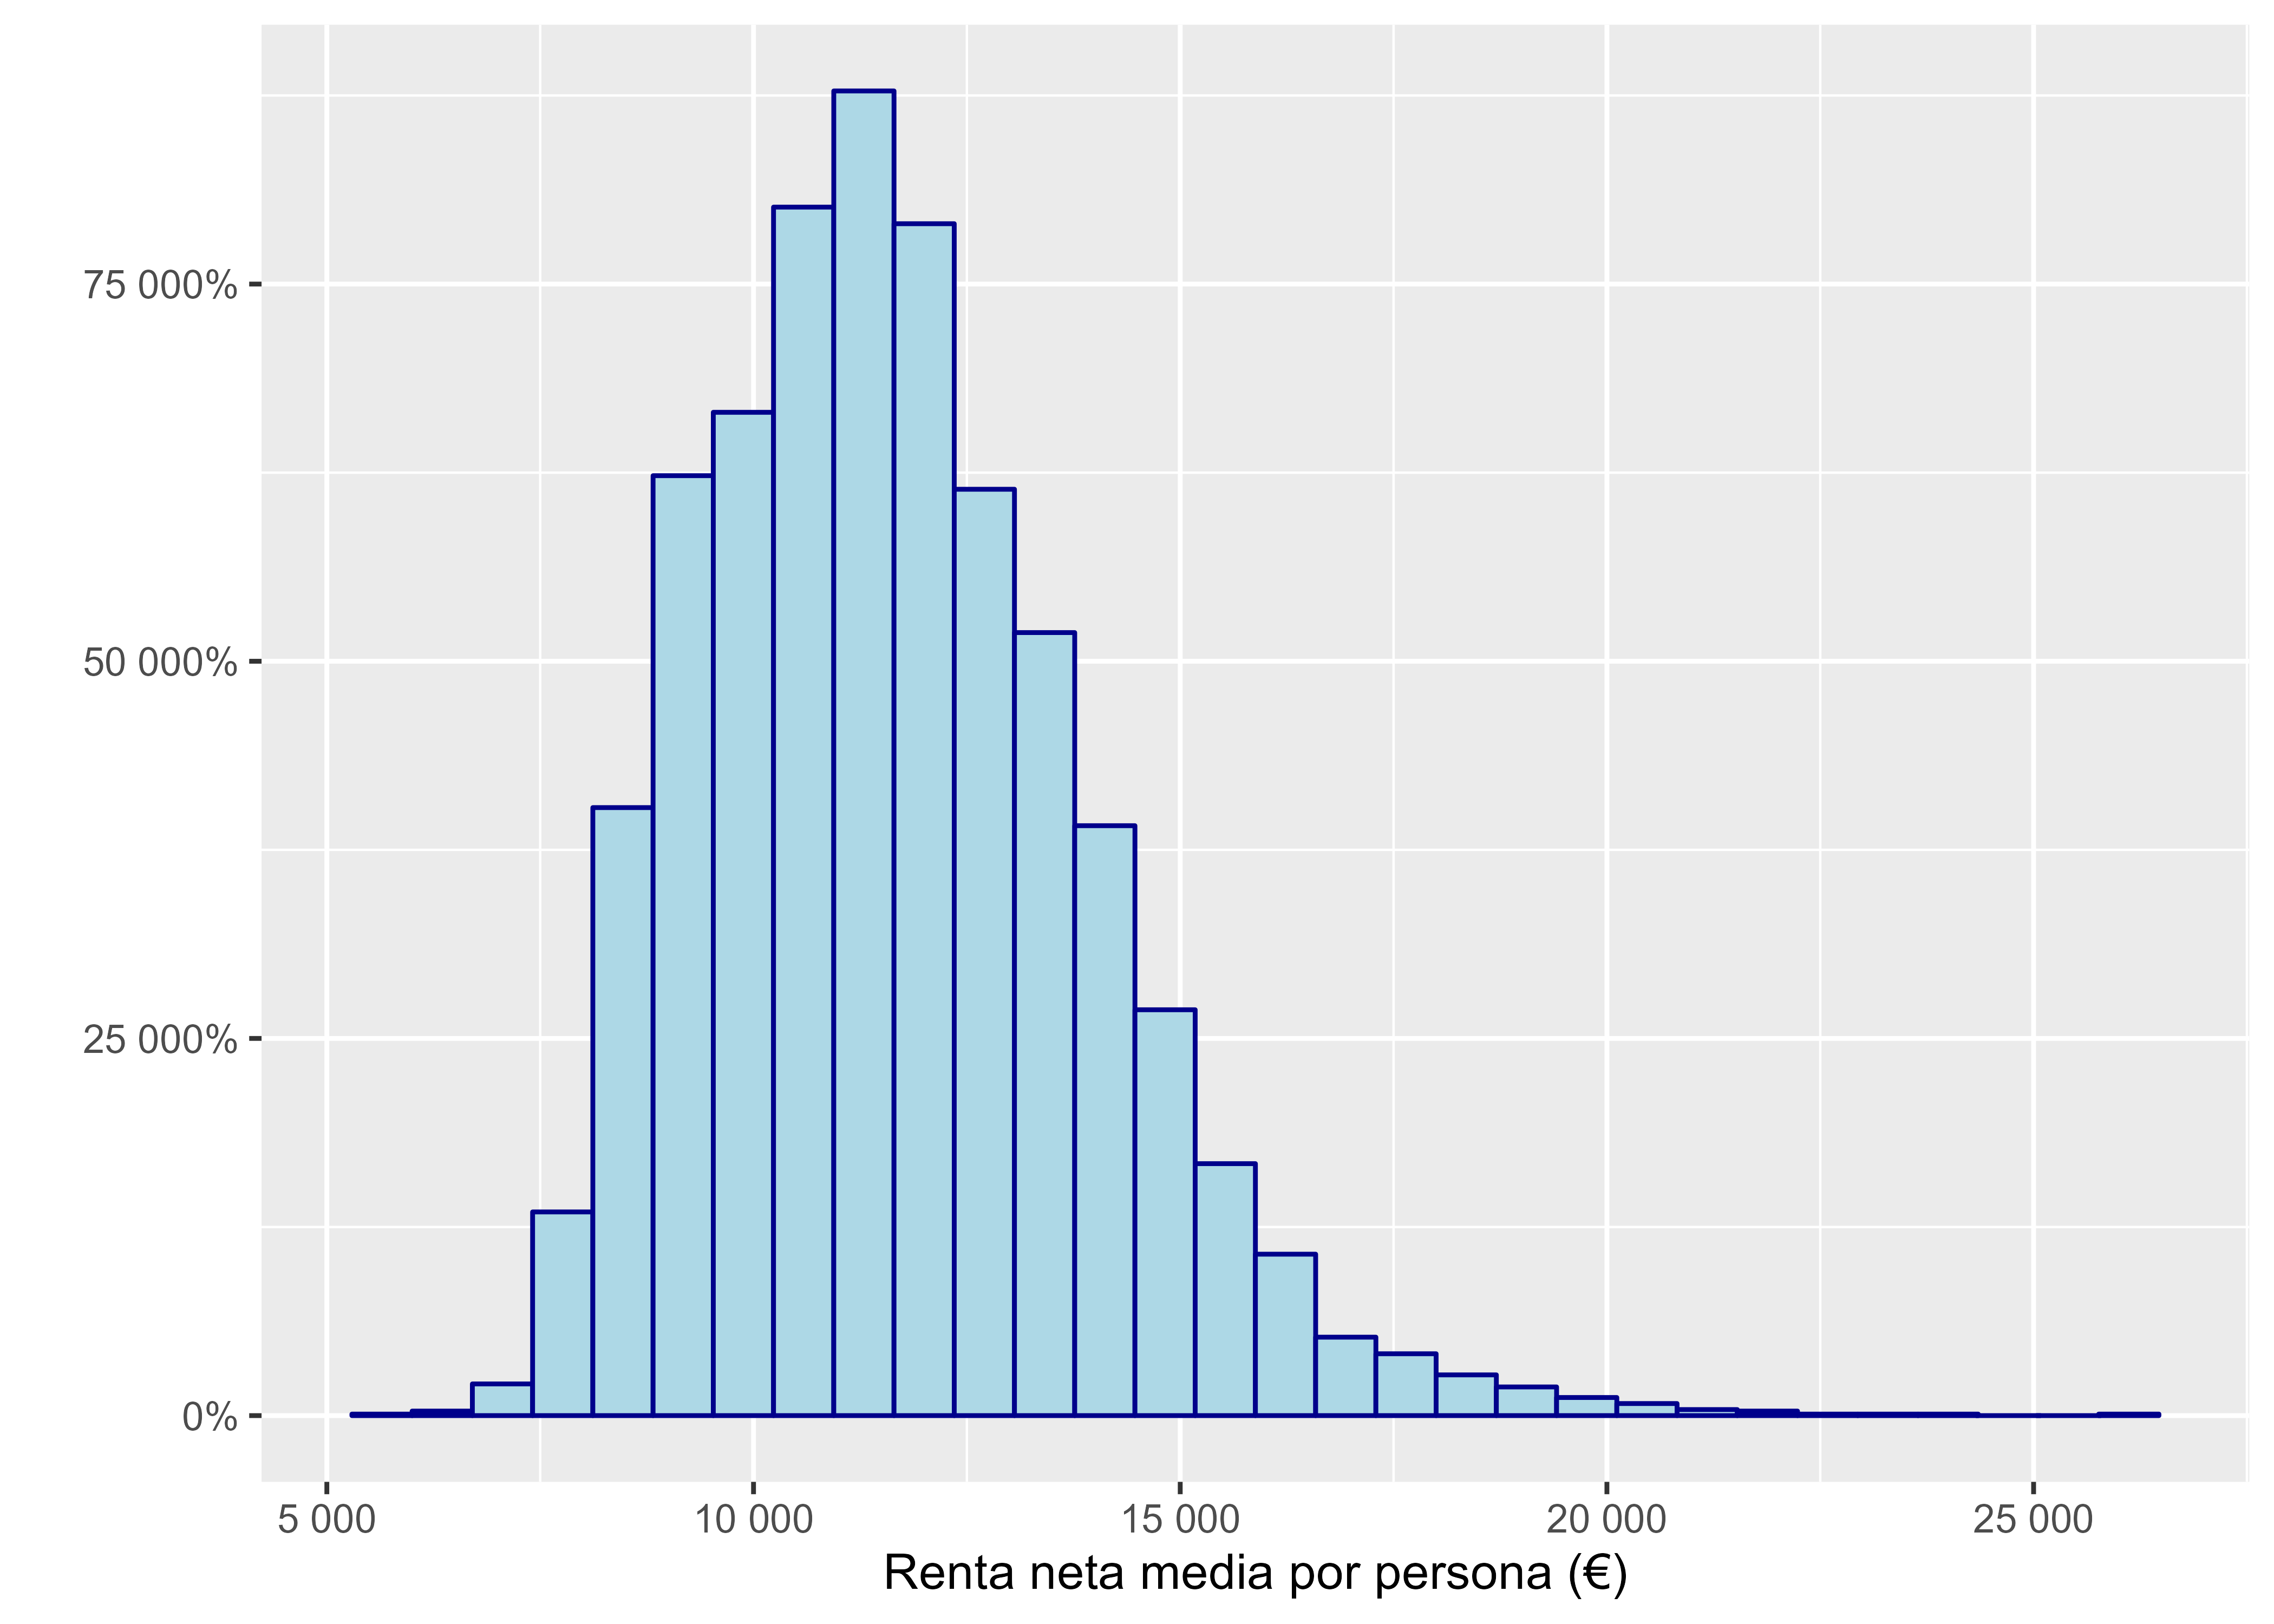
\includegraphics[width=0.6\linewidth]{_main_files/figure-latex/basic-1} 

}

\caption{Histograma de la variable Renta neta media por persona (€) en 2019}\label{fig:basic}
\end{figure}

Se puede observar que la renta presenta una distribución Gamma con un gran
número de municipios concentrados en zonas medias de renta y pocos municipios en tramos de
rentas altas. Como se verá en el Ejercicio XXX, esta distribución va a afectar a la
información que transmite el mapa.

::: \{.exercise \#ex20 name='' Mapa de coropletas de la distribución de la renta'' \}
Realice un mapa de coropletas mostrando la distribución de la
renta usando los valores brutos de renta sin modificar
:::

\begin{Shaded}
\begin{Highlighting}[]

\FunctionTok{ggplot}\NormalTok{(munis\_renta) }\SpecialCharTok{+}
  \CommentTok{\# Usamos geom\_sf, y como aes() lo que queremos mostrar, en este caso, el}
  \CommentTok{\# color del polígono representa la renta. Vamos a retirar los bordes con}
  \CommentTok{\# color = NA}
  \FunctionTok{geom\_sf}\NormalTok{(}\FunctionTok{aes}\NormalTok{(}\AttributeTok{fill =} \StringTok{\textasciigrave{}}\AttributeTok{2019}\StringTok{\textasciigrave{}}\NormalTok{), }\AttributeTok{color =} \ConstantTok{NA}\NormalTok{) }\SpecialCharTok{+}
  \FunctionTok{theme\_minimal}\NormalTok{() }\SpecialCharTok{+}
  \FunctionTok{scale\_fill\_continuous}\NormalTok{(}\AttributeTok{labels =}\NormalTok{ scales}\SpecialCharTok{::}\FunctionTok{label\_number}\NormalTok{(}
    \AttributeTok{big.mark =} \StringTok{"."}\NormalTok{,}
    \AttributeTok{decimal.mark =} \StringTok{","}\NormalTok{,}
    \AttributeTok{suffix =} \StringTok{" €"}
\NormalTok{  )) }\CommentTok{\# +}
\end{Highlighting}
\end{Shaded}

\begin{figure}

{\centering 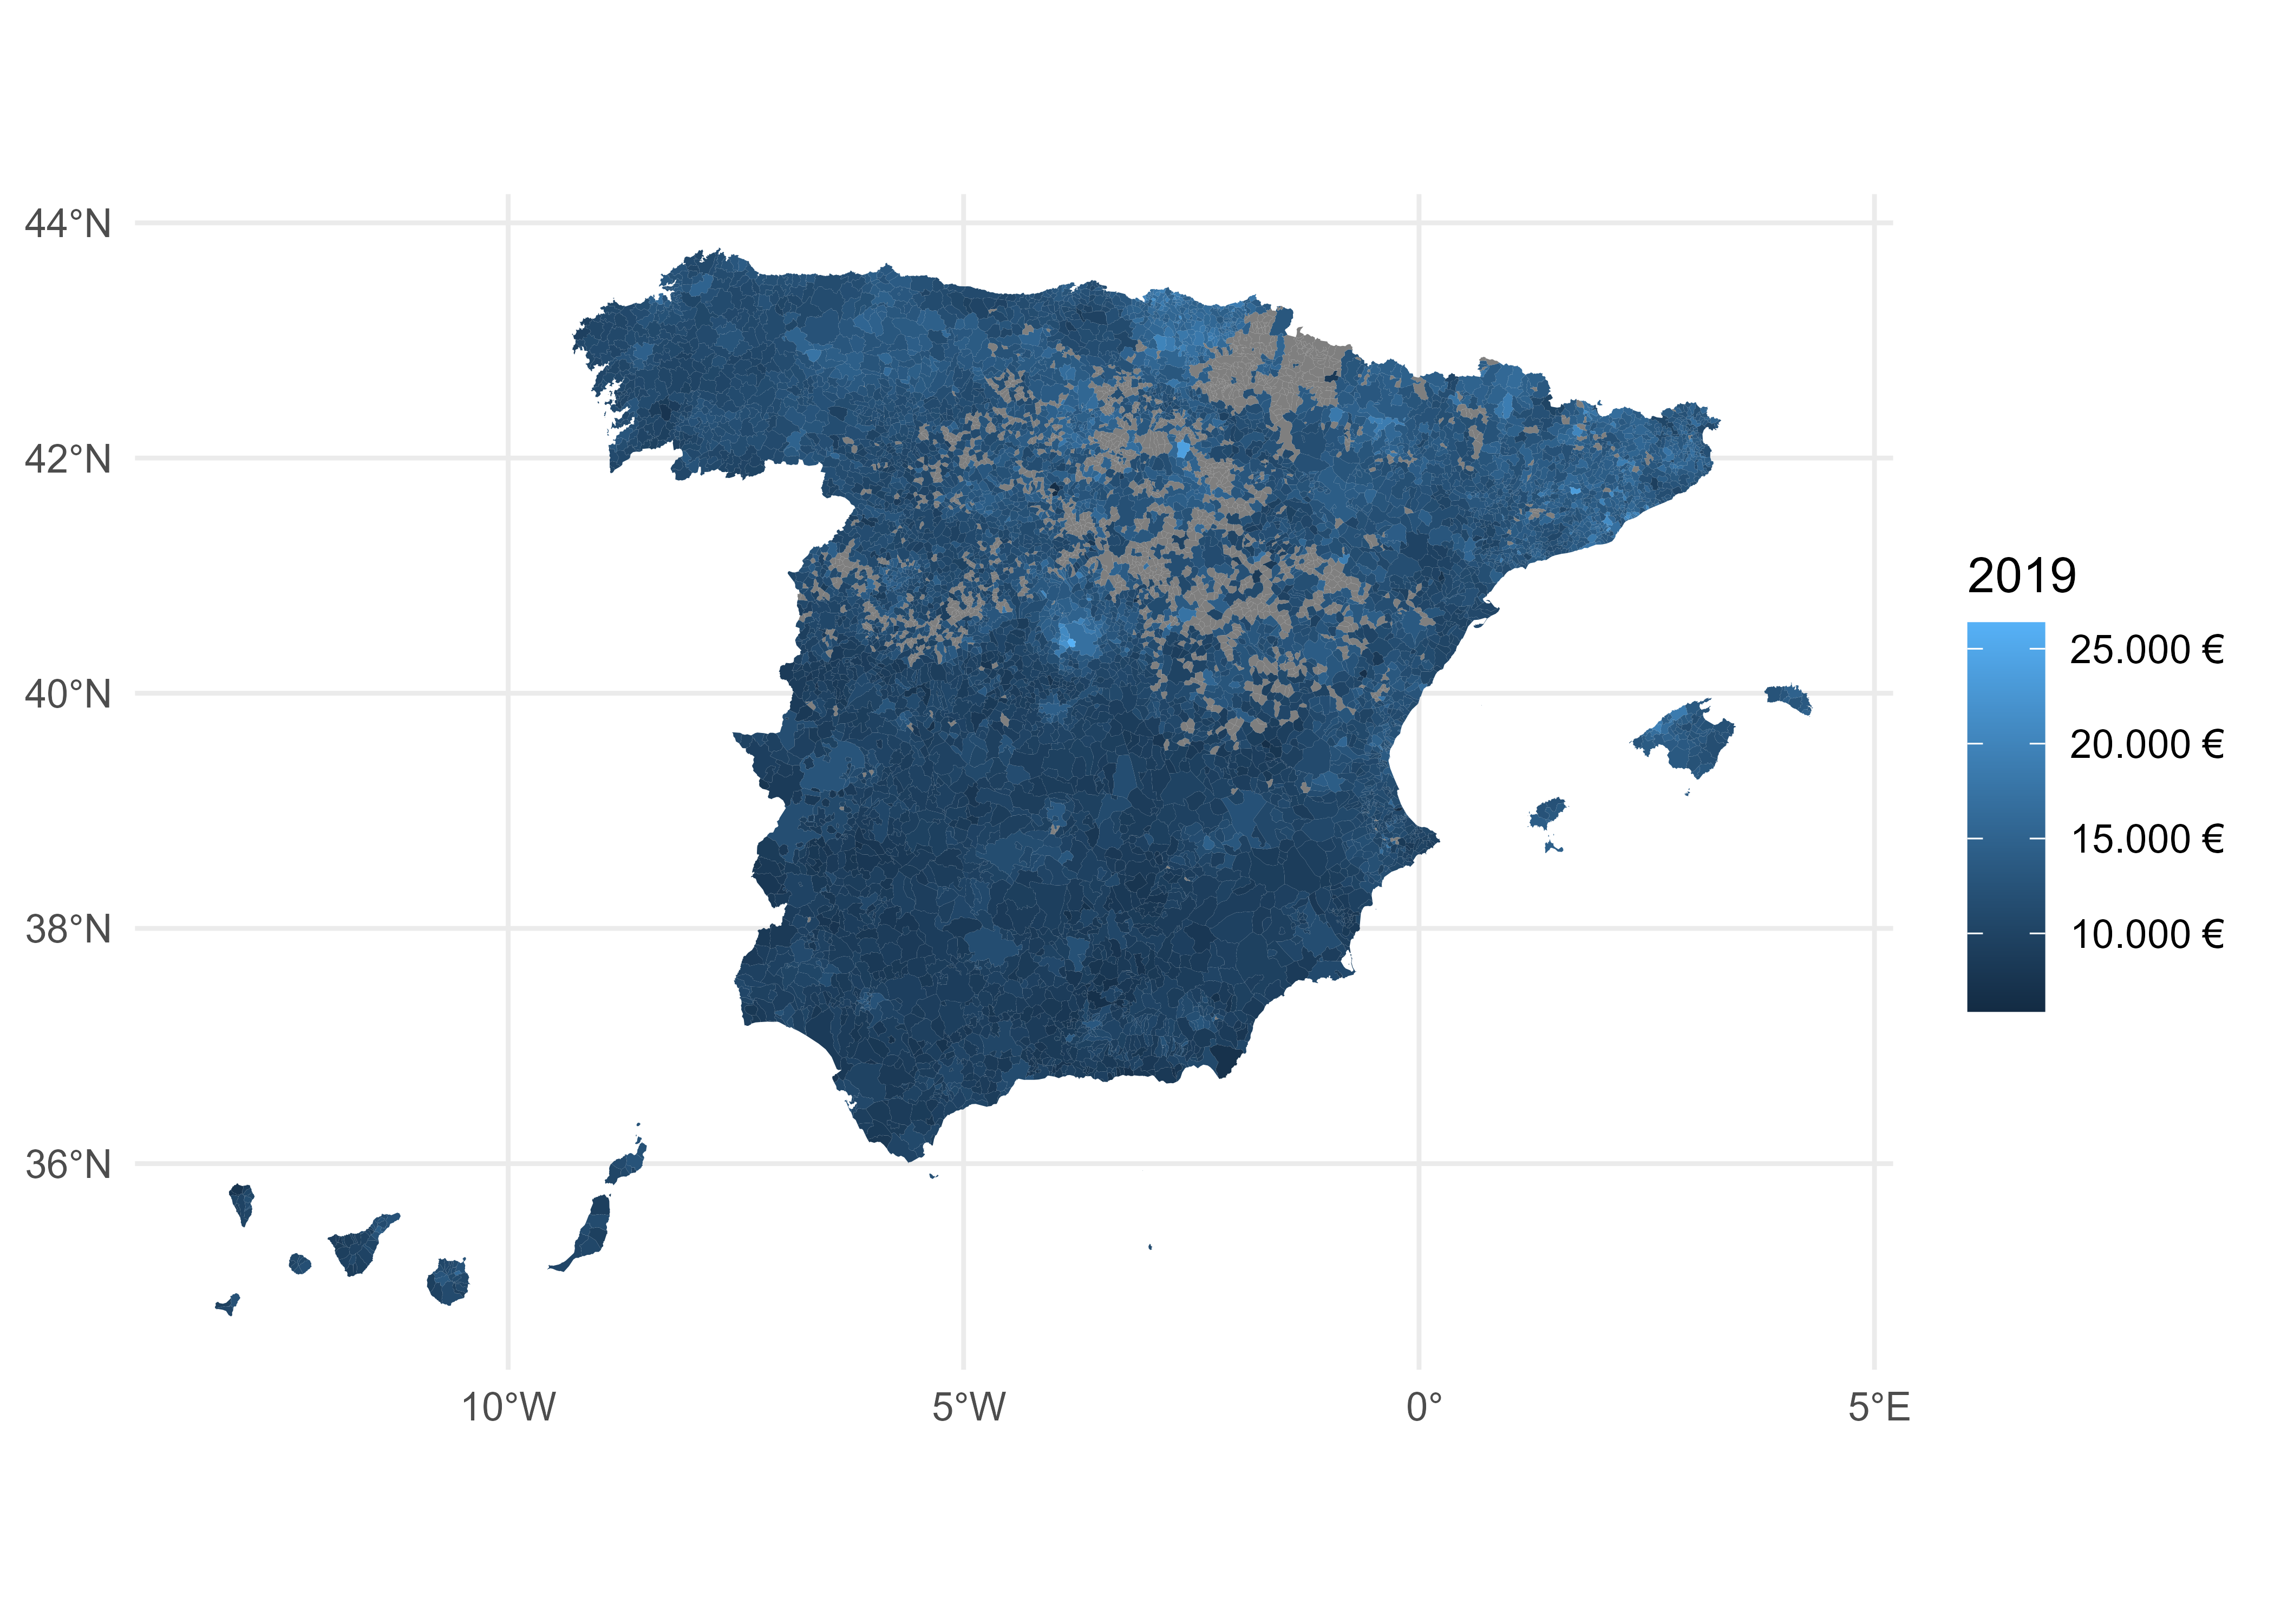
\includegraphics[width=0.6\linewidth]{_main_files/figure-latex/maparenta1-1} 

}

\caption{Renta neta media por persona en España (2019)}\label{fig:maparenta1}
\end{figure}

\begin{Shaded}
\begin{Highlighting}[]
\CommentTok{\# labs(}
\CommentTok{\#  title = "Renta neta media por persona",}
\CommentTok{\#  caption = "Datos: INE"}
\CommentTok{\# )}
\end{Highlighting}
\end{Shaded}

Este primer mapa no es demasiado informativo, por los siguientes motivos:

\begin{itemize}
\item
  Existe una serie de municipios para los que no tenemos datos.
\item
  La escala de color no es la más adecuada.
\item
  Dada la distribución de los datos, puede ser adecuado crear grupos de renta
  para que el mapa sea más interpretable.
\end{itemize}

\begin{exercise}[Adecuacion de los datos al la visualización]
\protect\hypertarget{exr:ex21}{}\label{exr:ex21}Elimine los municipios sin datos y a cambie la escala de
color para ver si mejora la visualización de la variable Renta neta media por persona.
\end{exercise}

\begin{Shaded}
\begin{Highlighting}[]

\NormalTok{munis\_renta\_clean }\OtherTok{\textless{}{-}}\NormalTok{ munis\_renta }\SpecialCharTok{\%\textgreater{}\%} \FunctionTok{filter}\NormalTok{(}\SpecialCharTok{!}\FunctionTok{is.na}\NormalTok{(}\StringTok{\textasciigrave{}}\AttributeTok{2019}\StringTok{\textasciigrave{}}\NormalTok{))}

\FunctionTok{ggplot}\NormalTok{(munis\_renta\_clean) }\SpecialCharTok{+}
  \FunctionTok{geom\_sf}\NormalTok{(}\FunctionTok{aes}\NormalTok{(}\AttributeTok{fill =} \StringTok{\textasciigrave{}}\AttributeTok{2019}\StringTok{\textasciigrave{}}\NormalTok{), }\AttributeTok{color =} \ConstantTok{NA}\NormalTok{) }\SpecialCharTok{+}
  \CommentTok{\# Cambiamos la paleta de colores, vamos a usar una paleta denominada Inferno,}
  \CommentTok{\# ya incluida en base R con hcl.colors}

  \CommentTok{\# Como son datos continuos, puedo usar Inferno}
  \FunctionTok{scale\_fill\_gradientn}\NormalTok{(}
    \AttributeTok{colours =} \FunctionTok{hcl.colors}\NormalTok{(}\DecValTok{20}\NormalTok{, }\StringTok{"Inferno"}\NormalTok{, }\AttributeTok{rev =} \ConstantTok{TRUE}\NormalTok{),}
    \AttributeTok{labels =}\NormalTok{ scales}\SpecialCharTok{::}\FunctionTok{label\_number}\NormalTok{(}
      \AttributeTok{big.mark =} \StringTok{"."}\NormalTok{,}
      \AttributeTok{decimal.mark =} \StringTok{","}\NormalTok{,}
      \AttributeTok{suffix =} \StringTok{" €"}
\NormalTok{    )}
\NormalTok{  ) }\SpecialCharTok{+}
  \FunctionTok{theme\_minimal}\NormalTok{()}
\end{Highlighting}
\end{Shaded}

\begin{figure}

{\centering 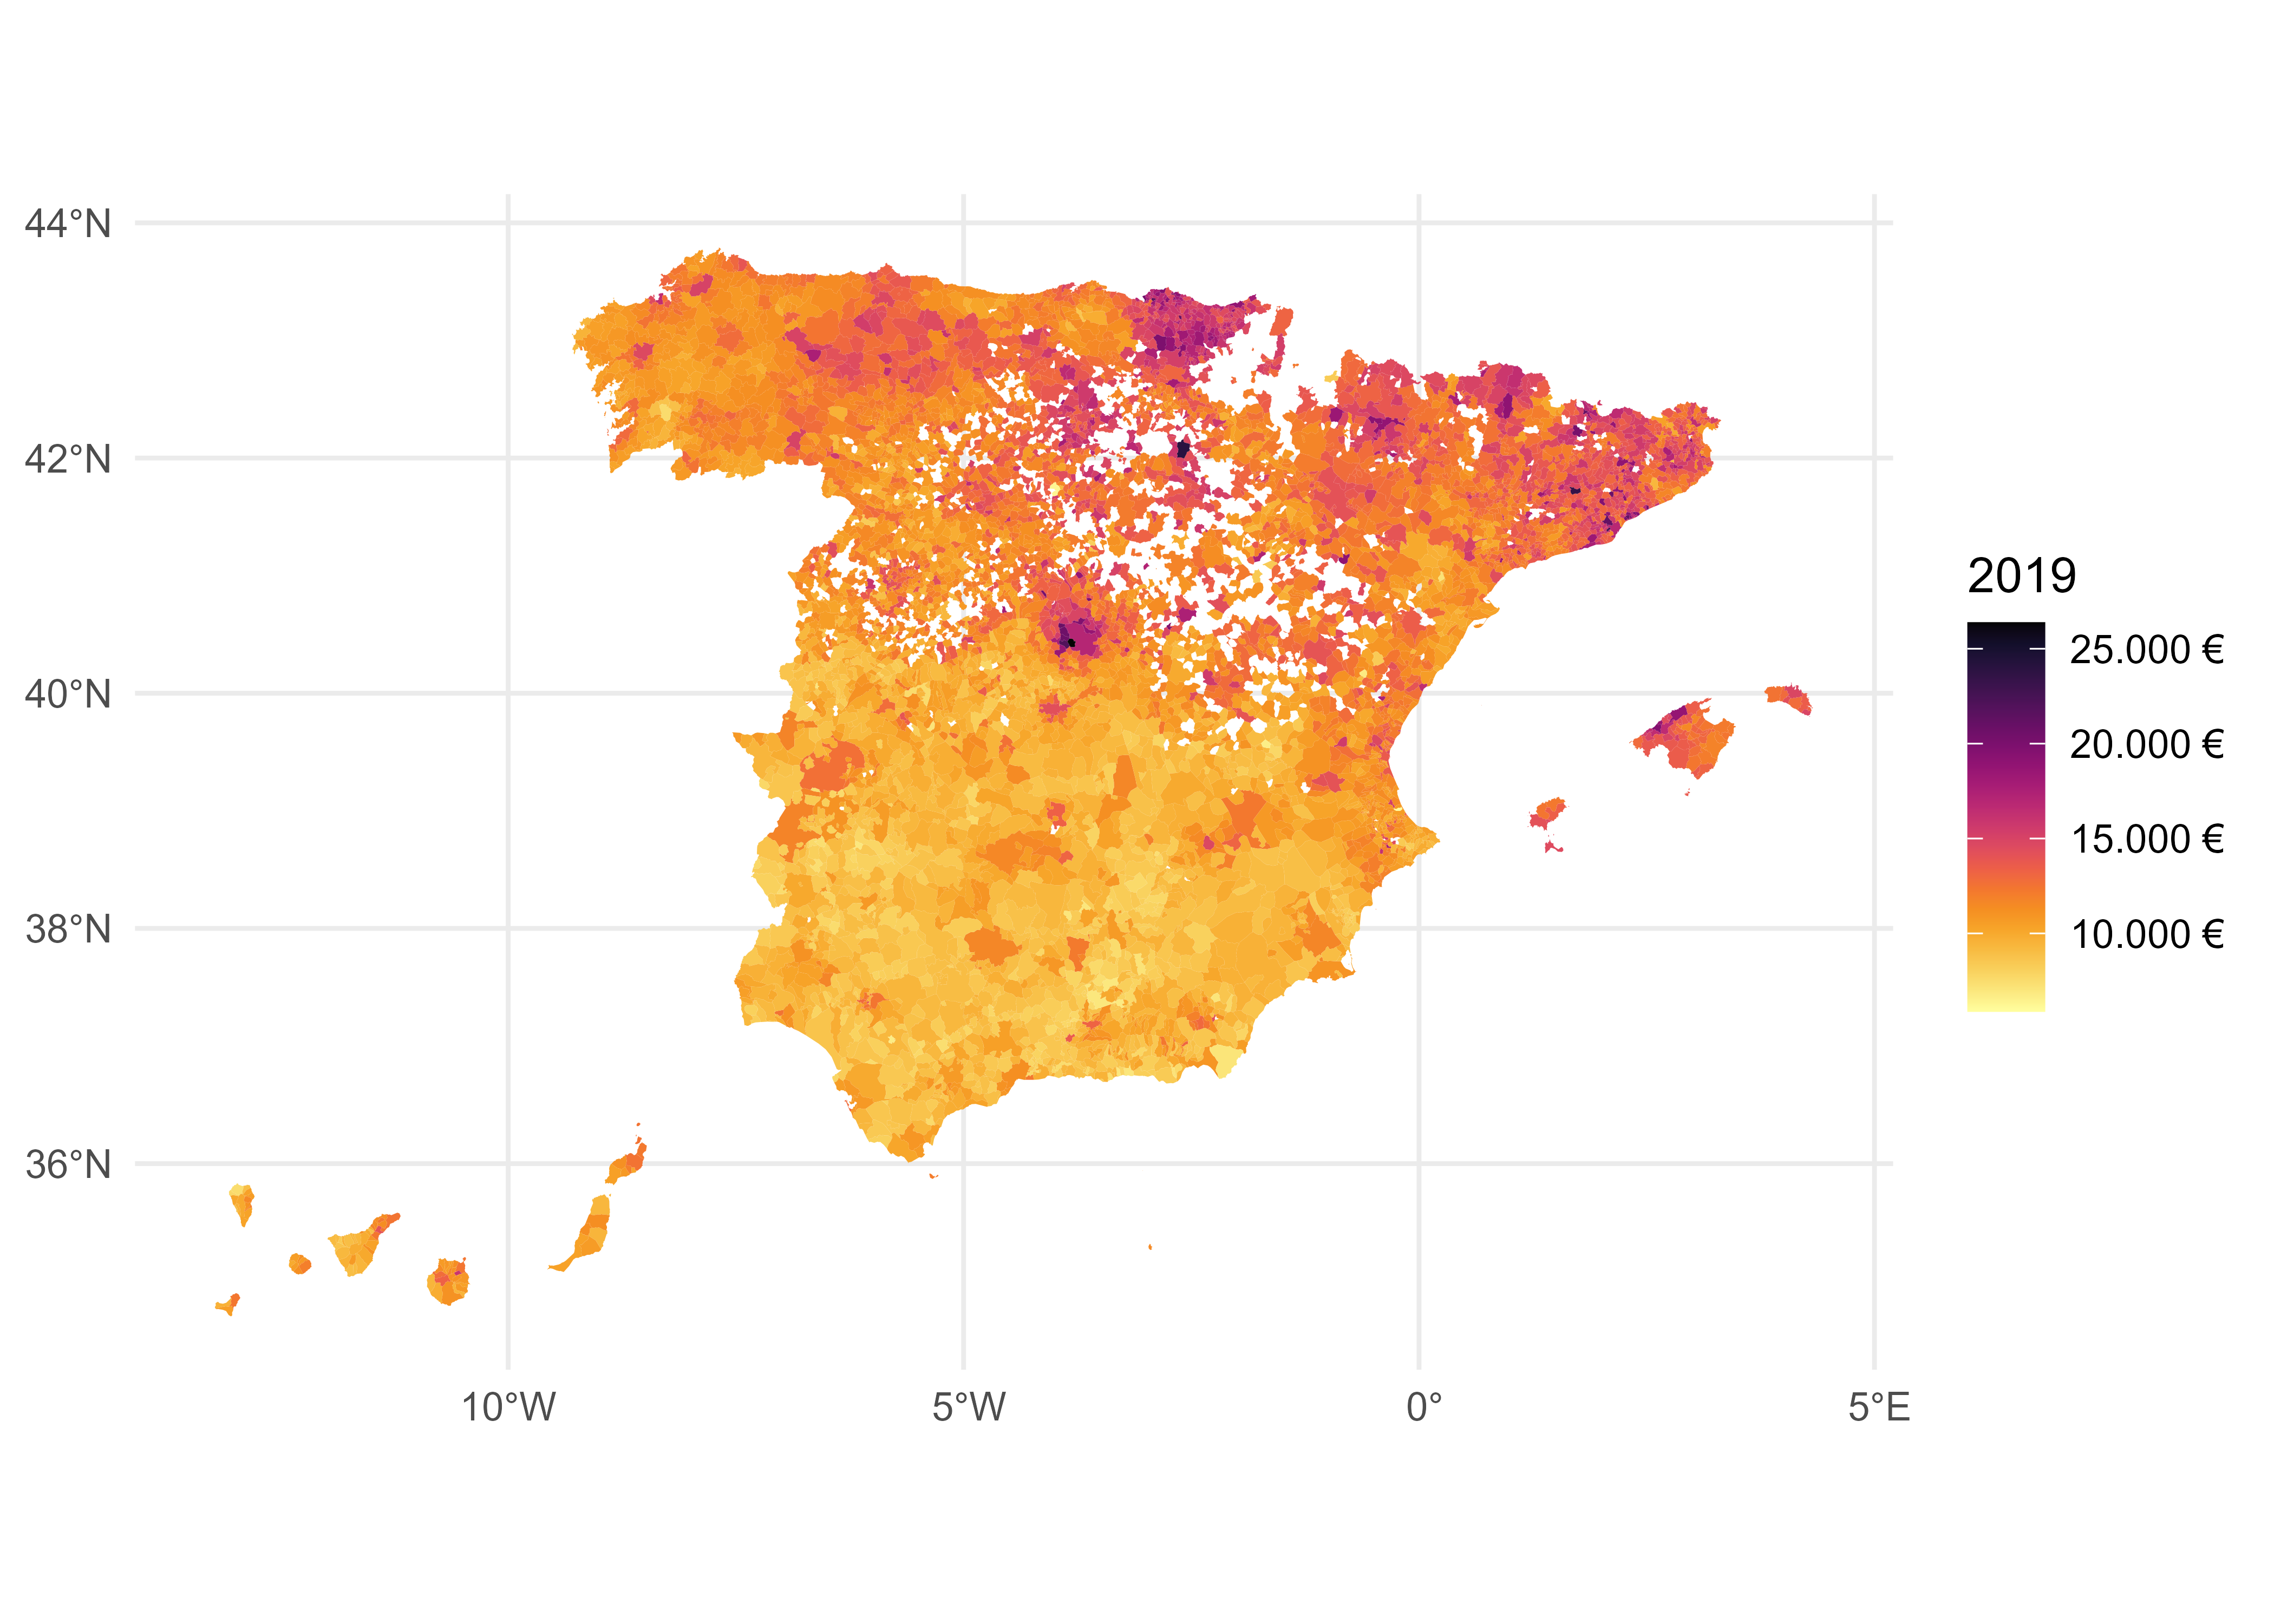
\includegraphics[width=0.6\linewidth]{_main_files/figure-latex/maparenta2-1} 

}

\caption{Renta neta media por persona en España (2019)}\label{fig:maparenta2}
\end{figure}

\begin{Shaded}
\begin{Highlighting}[]
\CommentTok{\# + labs(}
\CommentTok{\#    title = "Renta neta media por persona",}
\CommentTok{\#    caption = "Datos: INE"}
\CommentTok{\#  )}
\end{Highlighting}
\end{Shaded}

Este mapa proporciona algo más de información, y parece intuirse que las rentas más
altas se encuentran en zonas de País Vasco, Madrid y Cataluña. Sin embargo, el
hecho de que la distribución de los datos no sea normal está afectando a la
visualización.

Para intentar atajar este problema, se puede dividir los datos en clases,
por ejemplo, cuartiles o deciles. Existen varios métodos de clasificación de
datos, que en R se encuentran implementados en el paquete \texttt{classInt}. A
continuación se van a plantear diversos métodos de clasificación y se
observará cómo la ``historia'' que cuenta el mapa varía en función de dichas
clases. Se proponen siguientes métodos de clasificación:

\begin{itemize}
\item
  \textbf{El método de deciles}: consiste en crear 10 categorías incluyendo el mismo
  número de registros en cada una de ellas.
\item
  \textbf{El método de intervalos equivalentes}: divide el rango de valores en un
  número de grupos definido. La distancia de todos los intervalos es idéntica,
  por lo que este método no tiene en cuenta la distribución de los registros.
\item
  \textbf{El método de Fisher-Jenks}: desarrollado específicamente para la
  clasificación de datos espaciales y su visualización en mapas. Produce
  agrupaciones de tal manera que los datos de cada grupo son ``cercanas'' entre
  sí y sustancialmente distintas de los valores de otros grupos.
\end{itemize}

\begin{exercise}[División de los datos en clases]
\protect\hypertarget{exr:ex22}{}\label{exr:ex22}Utilice la función \texttt{classIntervals} del paquete \texttt{classInt}
y cambie el parámetro \texttt{style} para obtener los métodos de
clasificación: Deciles, tramos de Renta equidistantes y Fisher and Jenks.

Realice un \texttt{plot} de las clases obtenidas y compárelas.
\end{exercise}

\begin{Shaded}
\begin{Highlighting}[]

\FunctionTok{library}\NormalTok{(classInt)}

\CommentTok{\# División en deciles}
\NormalTok{deciles }\OtherTok{\textless{}{-}} \FunctionTok{classIntervals}\NormalTok{(munis\_renta\_clean}\SpecialCharTok{$}\StringTok{\textasciigrave{}}\AttributeTok{2019}\StringTok{\textasciigrave{}}\NormalTok{,}
  \AttributeTok{style =} \StringTok{"quantile"}\NormalTok{, }\AttributeTok{n =} \DecValTok{10}
\NormalTok{)}
\NormalTok{deciles}
\CommentTok{\#\textgreater{} style: quantile}
\CommentTok{\#\textgreater{}     [5898,8935.6)   [8935.6,9662.2)  [9662.2,10352.8)   [10352.8,10918) }
\CommentTok{\#\textgreater{}               656               656               655               654 }
\CommentTok{\#\textgreater{}     [10918,11462)   [11462,11998.6) [11998.6,12651.4) [12651.4,13475.8) }
\CommentTok{\#\textgreater{}               655               658               656               655 }
\CommentTok{\#\textgreater{} [13475.8,14618.4)   [14618.4,26367] }
\CommentTok{\#\textgreater{}               656               656}
\FunctionTok{plot}\NormalTok{(deciles, }\AttributeTok{pal =} \FunctionTok{hcl.colors}\NormalTok{(}\DecValTok{20}\NormalTok{, }\StringTok{"Inferno"}\NormalTok{), }\AttributeTok{main =} \StringTok{"Deciles"}\NormalTok{)}
\end{Highlighting}
\end{Shaded}

\begin{center}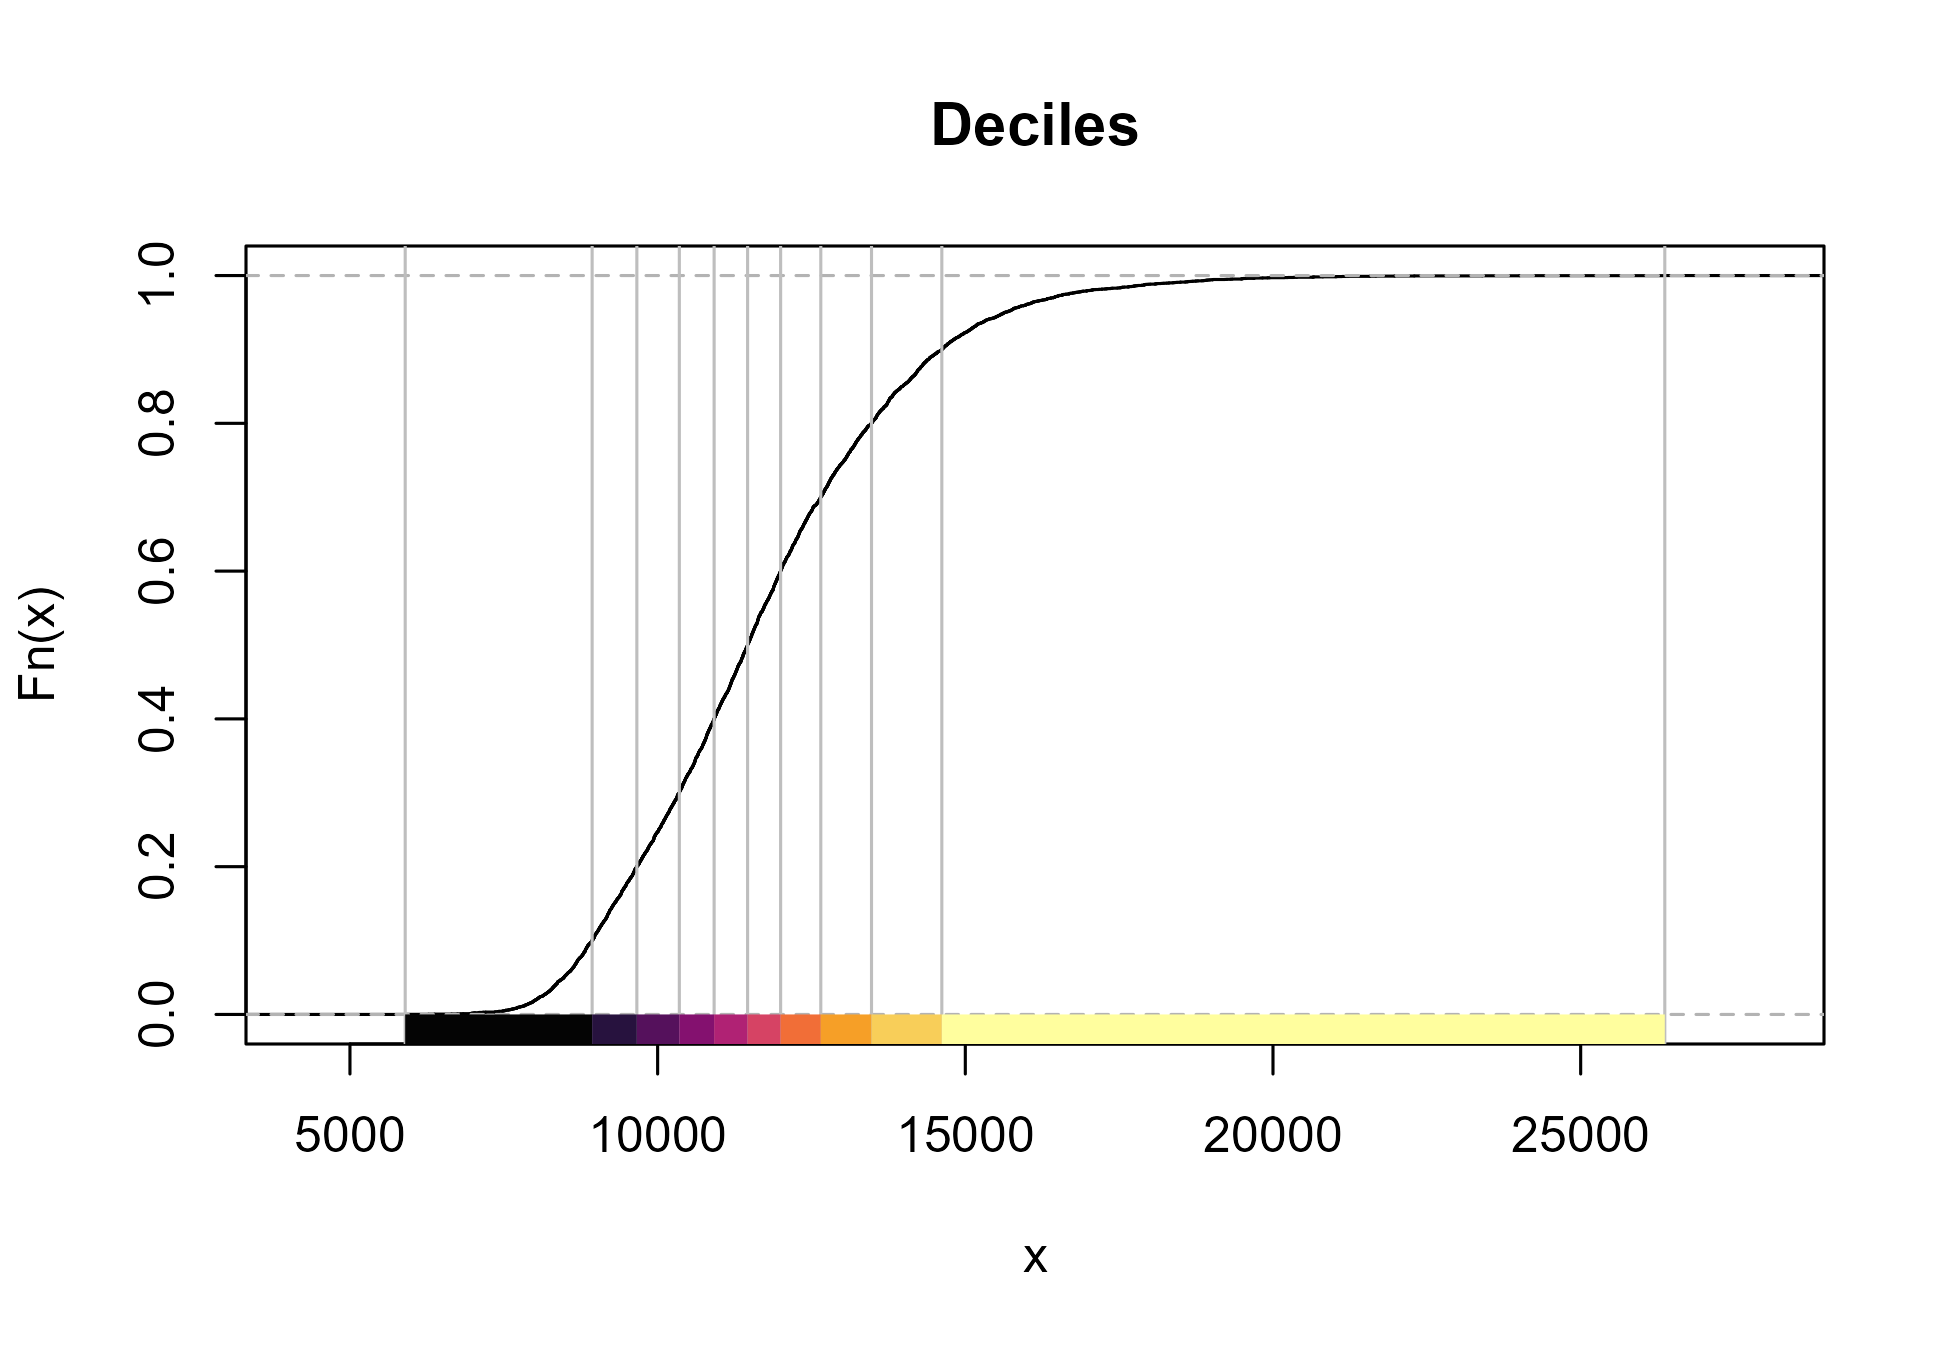
\includegraphics[width=0.6\linewidth]{_main_files/figure-latex/classint-1} \end{center}

\begin{Shaded}
\begin{Highlighting}[]


\CommentTok{\# Tramos equidistantes en términos de renta}
\NormalTok{equal }\OtherTok{\textless{}{-}} \FunctionTok{classIntervals}\NormalTok{(munis\_renta\_clean}\SpecialCharTok{$}\StringTok{\textasciigrave{}}\AttributeTok{2019}\StringTok{\textasciigrave{}}\NormalTok{,}
  \AttributeTok{style =} \StringTok{"equal"}\NormalTok{, }\AttributeTok{n =} \DecValTok{10}
\NormalTok{)}
\NormalTok{equal}
\CommentTok{\#\textgreater{} style: equal}
\CommentTok{\#\textgreater{}     [5898,7944.9)   [7944.9,9991.8)  [9991.8,12038.7) [12038.7,14085.6) }
\CommentTok{\#\textgreater{}               103              1510              2374              1637 }
\CommentTok{\#\textgreater{} [14085.6,16132.5) [16132.5,18179.4) [18179.4,20226.3) [20226.3,22273.2) }
\CommentTok{\#\textgreater{}               702               161                52                14 }
\CommentTok{\#\textgreater{} [22273.2,24320.1)   [24320.1,26367] }
\CommentTok{\#\textgreater{}                 3                 1}
\FunctionTok{plot}\NormalTok{(equal, }\AttributeTok{pal =} \FunctionTok{hcl.colors}\NormalTok{(}\DecValTok{20}\NormalTok{, }\StringTok{"Inferno"}\NormalTok{), }\AttributeTok{main =} \StringTok{"Equidistantes"}\NormalTok{)}
\end{Highlighting}
\end{Shaded}

\begin{center}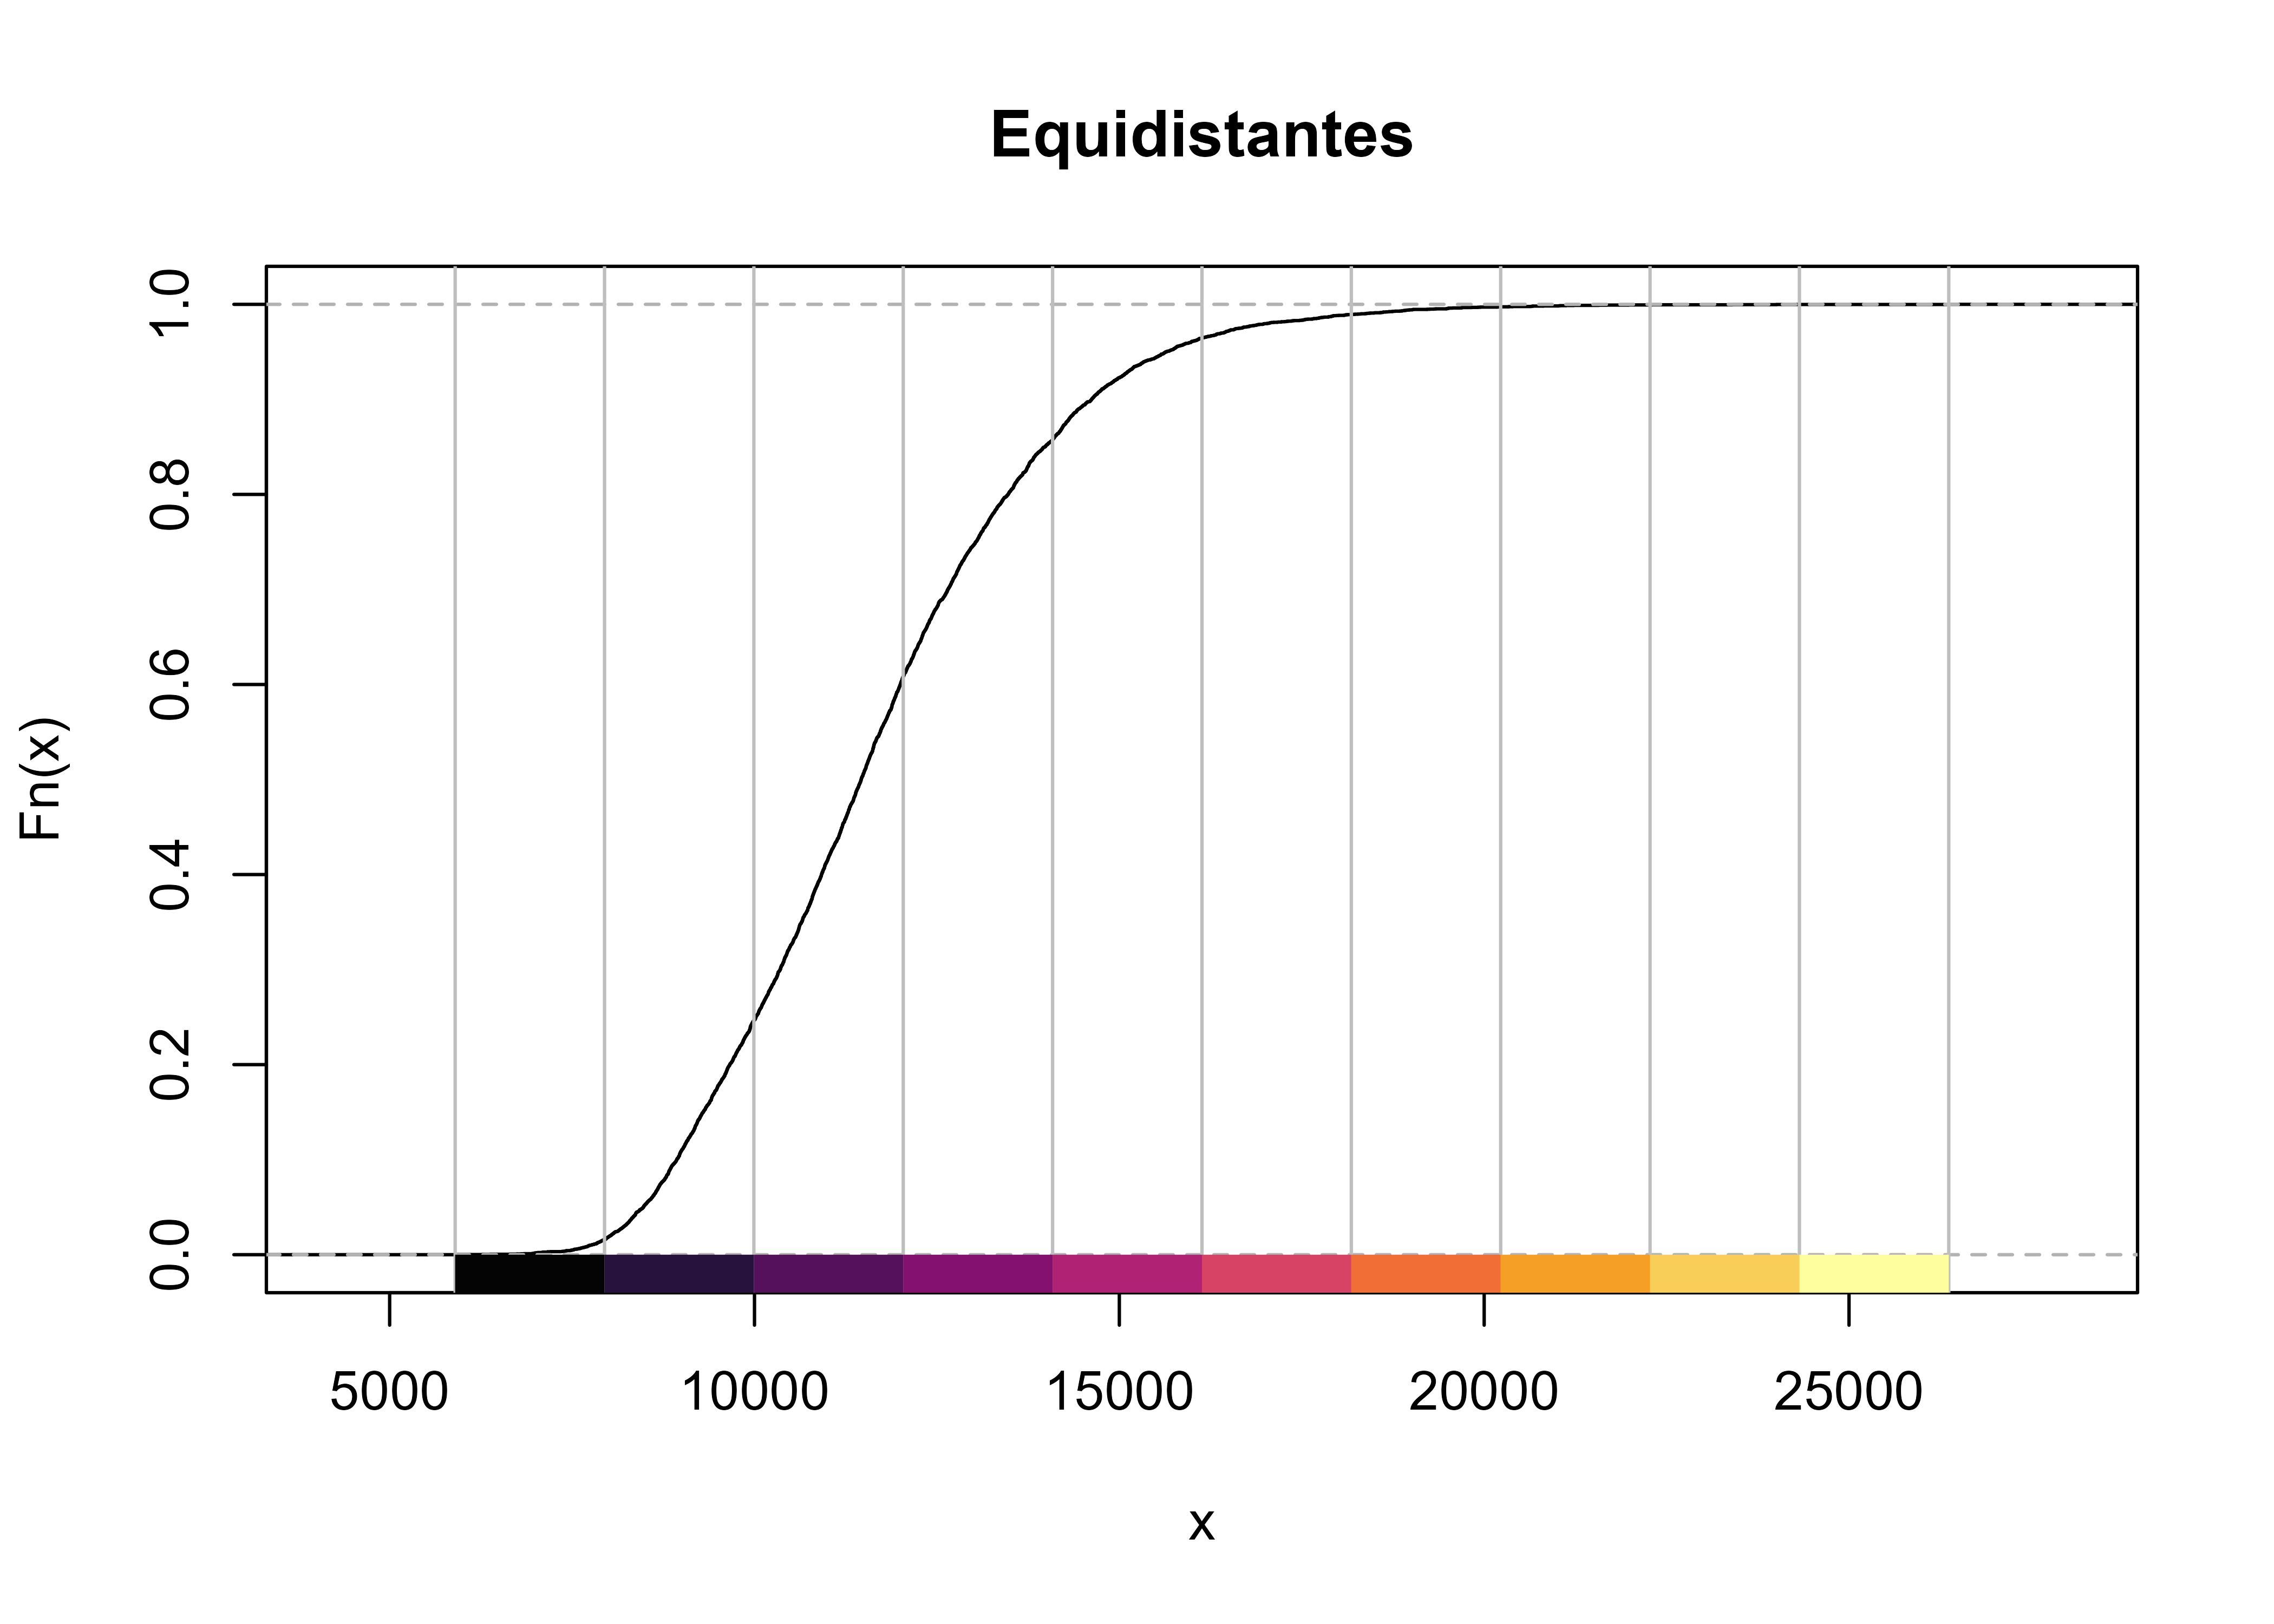
\includegraphics[width=0.6\linewidth]{_main_files/figure-latex/classint-2} \end{center}

\begin{Shaded}
\begin{Highlighting}[]

\NormalTok{fisher }\OtherTok{\textless{}{-}} \FunctionTok{classIntervals}\NormalTok{(munis\_renta\_clean}\SpecialCharTok{$}\StringTok{\textasciigrave{}}\AttributeTok{2019}\StringTok{\textasciigrave{}}\NormalTok{,}
  \AttributeTok{style =} \StringTok{"fisher"}\NormalTok{,}
  \CommentTok{\# Fuerzo para mejorar la comparación entre métodos}
  \AttributeTok{n =} \DecValTok{10}
\NormalTok{)}
\NormalTok{fisher}
\CommentTok{\#\textgreater{} style: fisher}
\CommentTok{\#\textgreater{}       [5898,8743)     [8743,9770.5)    [9770.5,10754)     [10754,11689) }
\CommentTok{\#\textgreater{}               505               904              1005              1159 }
\CommentTok{\#\textgreater{}     [11689,12668)     [12668,13803)   [13803,15222.5) [15222.5,17196.5) }
\CommentTok{\#\textgreater{}              1032               874               651               305 }
\CommentTok{\#\textgreater{} [17196.5,20063.5)   [20063.5,26367] }
\CommentTok{\#\textgreater{}               103                19}
\FunctionTok{plot}\NormalTok{(fisher,}
  \AttributeTok{pal =} \FunctionTok{hcl.colors}\NormalTok{(}\DecValTok{20}\NormalTok{, }\StringTok{"Inferno"}\NormalTok{),}
  \AttributeTok{main =} \StringTok{"Fisher{-}Jenks"}
\NormalTok{)}
\end{Highlighting}
\end{Shaded}

\begin{center}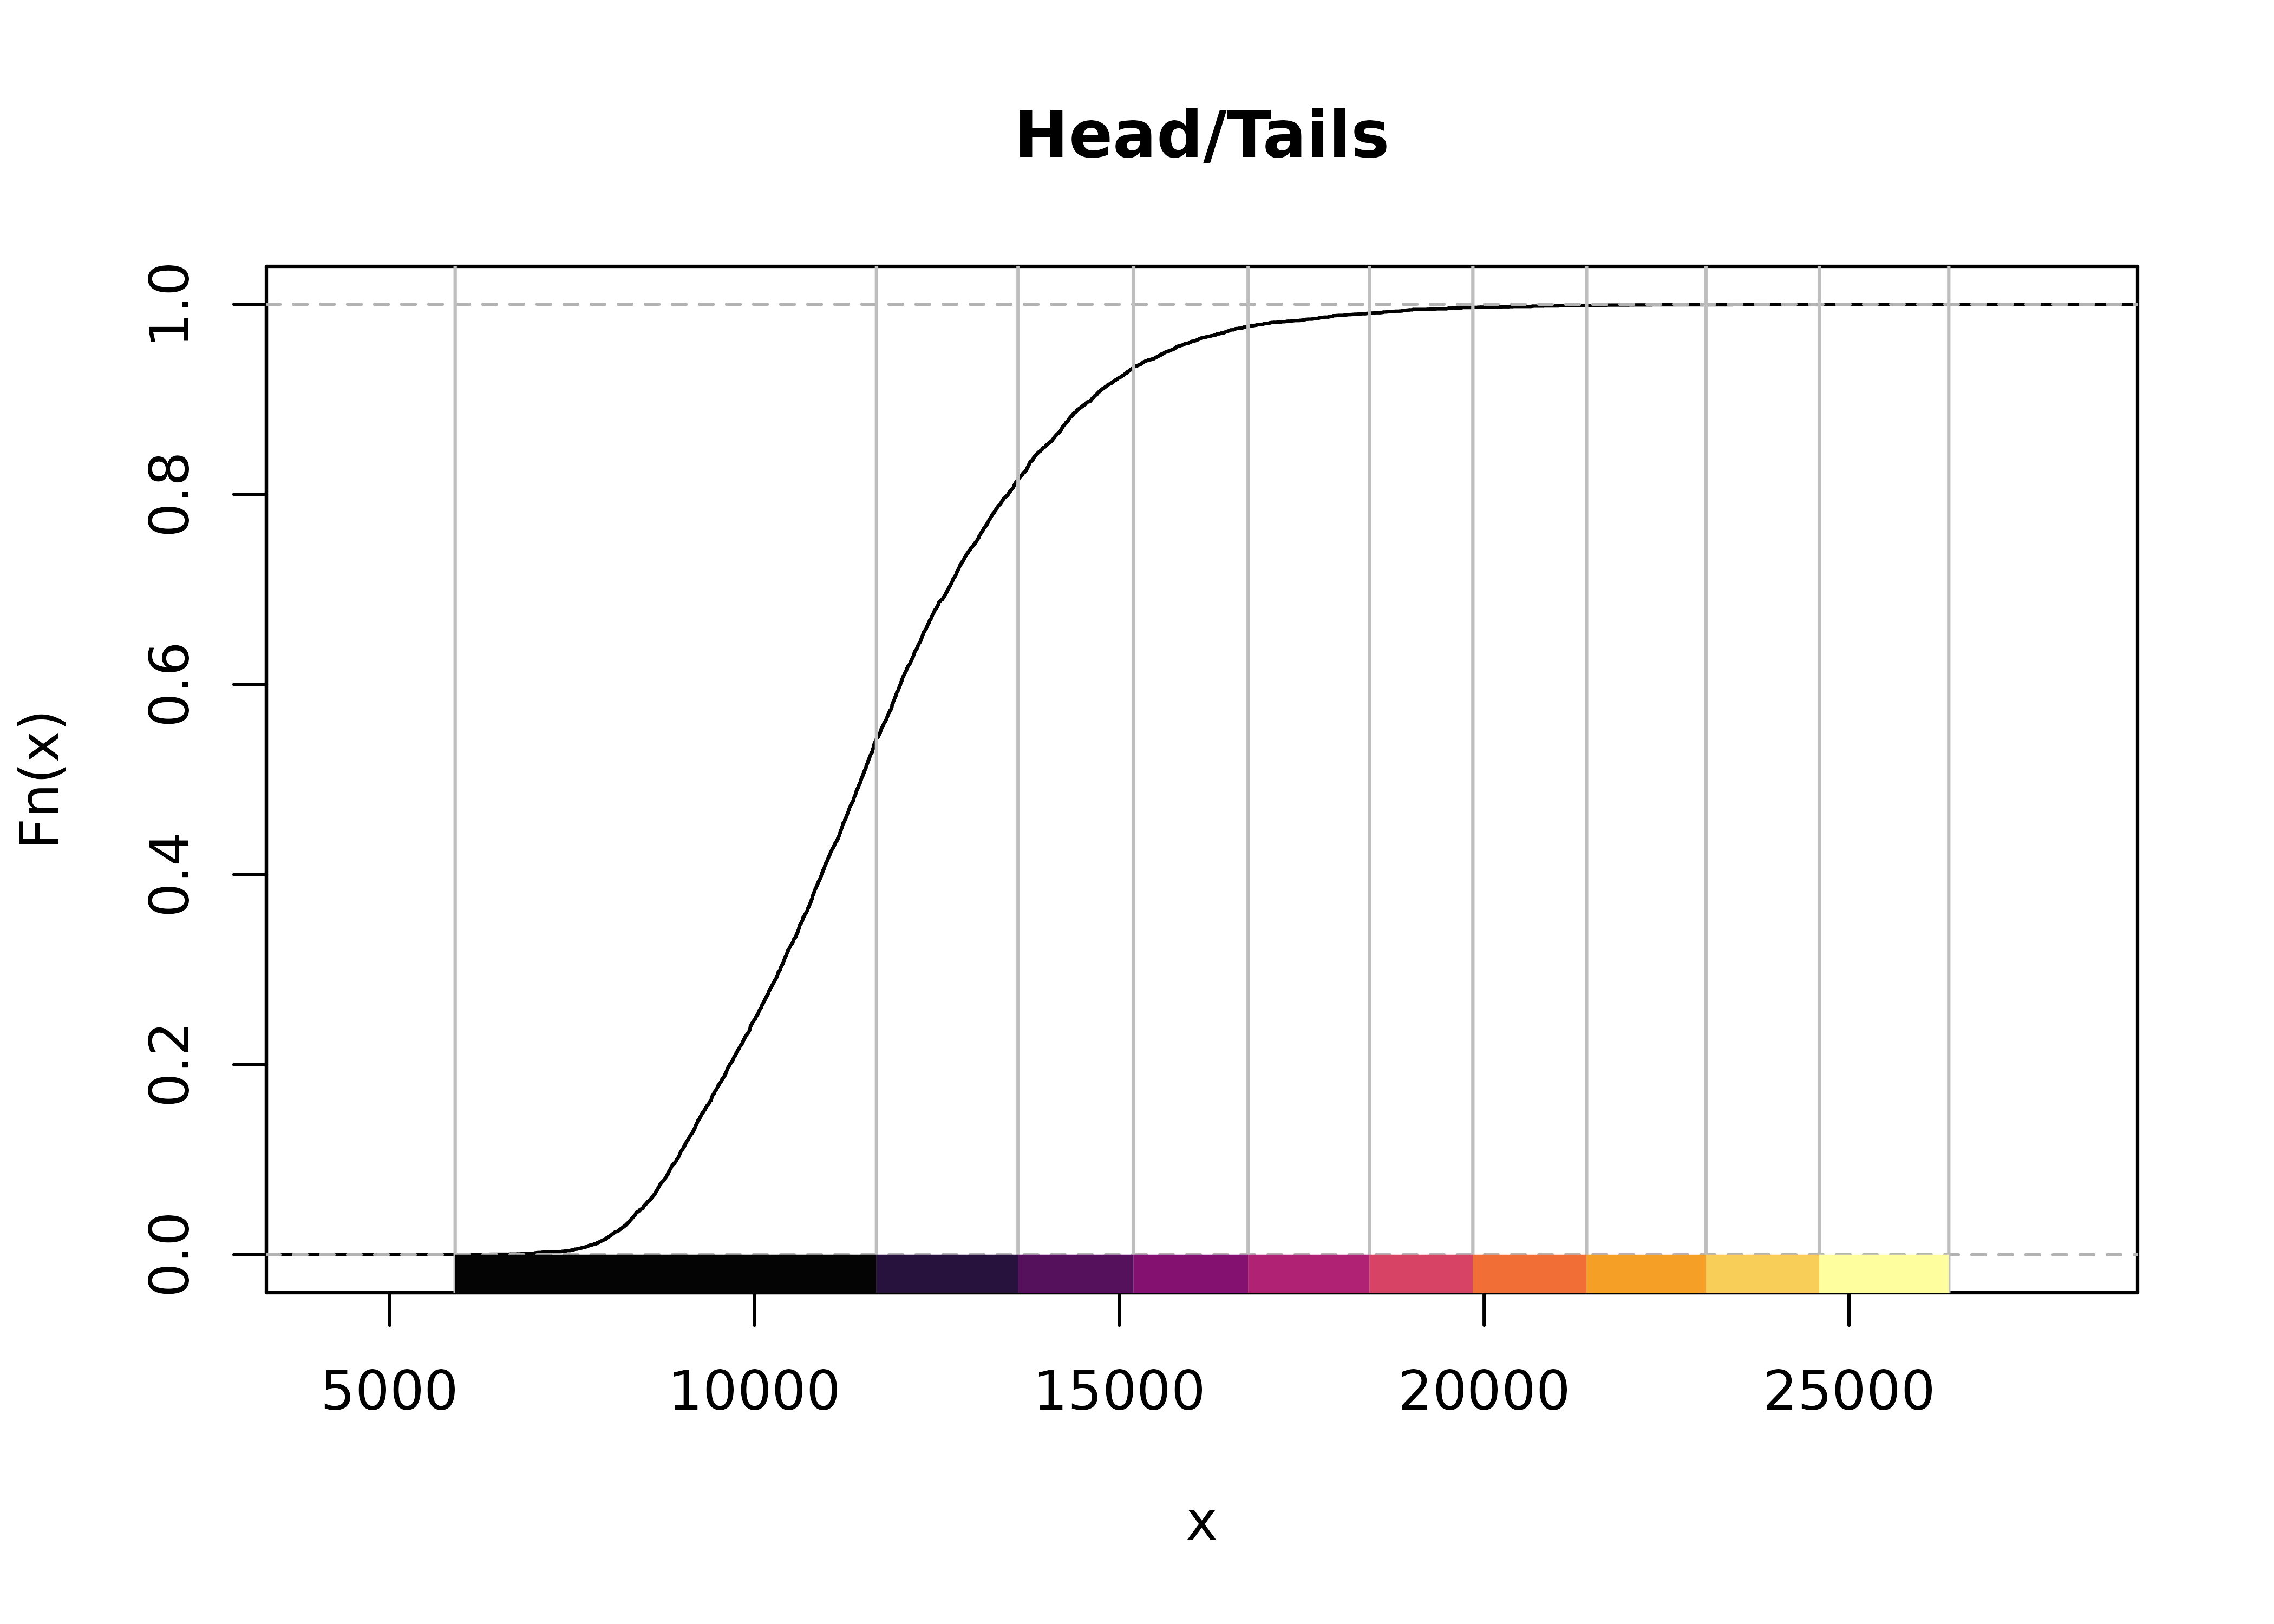
\includegraphics[width=0.6\linewidth]{_main_files/figure-latex/classint-3} \end{center}

Se puede observar lo siguiente:

\begin{itemize}
\item
  El último decil de renta se corresponde a un rango de entre 15.000 y 25.000
  €.
\item
  El método por deciles proporciona unos grupos con valores de renta muy
  parecidos entre sí en los valores medios. Esto es debido a la propia
  distribución de la variable.
\item
  El método de rangos equidistantes proporciona algunos grupos con un número
  muy reducido de municipios.
\item
  El método de Fisher-Jenks puede proporcionar unas clases con unos rangos más
  apropiados para los tramos altos de renta.
\end{itemize}

\begin{exercise}[Representación de los mapas según las clases obtenidas]
\protect\hypertarget{exr:ex23}{}\label{exr:ex23}Realice tres mapas distintos, creando clases de renta según cada uno
de los métodos anteriormente mostrados y coméntelos.
\end{exercise}

\textbf{Deciles}

\begin{Shaded}
\begin{Highlighting}[]
\CommentTok{\# Extracción de los valores de corte}
\NormalTok{breaks\_d }\OtherTok{\textless{}{-}}\NormalTok{ deciles}\SpecialCharTok{$}\NormalTok{brks}

\CommentTok{\# Creación de etiquetas básicas para cada clase}
\CommentTok{\# Creación de una función específica para crear etiquetas formateadas}
\NormalTok{label\_fun }\OtherTok{\textless{}{-}} \ControlFlowTok{function}\NormalTok{(x) \{}
\NormalTok{  l }\OtherTok{\textless{}{-}} \FunctionTok{length}\NormalTok{(x)}
\NormalTok{  eur }\OtherTok{\textless{}{-}} \FunctionTok{paste0}\NormalTok{(}\FunctionTok{prettyNum}\NormalTok{(}\FunctionTok{round}\NormalTok{(x, }\DecValTok{0}\NormalTok{),}
    \AttributeTok{decimal.mark =} \StringTok{","}\NormalTok{,}
    \AttributeTok{big.mark =} \StringTok{"."}
\NormalTok{  ), }\StringTok{" €"}\NormalTok{)}

\NormalTok{  labels }\OtherTok{\textless{}{-}} \FunctionTok{paste}\NormalTok{(eur[}\SpecialCharTok{{-}}\NormalTok{l], }\StringTok{"{-}"}\NormalTok{, eur[}\SpecialCharTok{{-}}\DecValTok{1}\NormalTok{])}
\NormalTok{  labels[}\DecValTok{1}\NormalTok{] }\OtherTok{\textless{}{-}} \FunctionTok{paste}\NormalTok{(}\StringTok{"\textless{}"}\NormalTok{, eur[}\DecValTok{1}\NormalTok{])}
\NormalTok{  labels[l }\SpecialCharTok{{-}} \DecValTok{1}\NormalTok{] }\OtherTok{\textless{}{-}} \FunctionTok{paste}\NormalTok{(}\StringTok{"\textgreater{}"}\NormalTok{, eur[l }\SpecialCharTok{{-}} \DecValTok{1}\NormalTok{])}
  \FunctionTok{return}\NormalTok{(labels)}
\NormalTok{\}}

\NormalTok{labels\_d }\OtherTok{\textless{}{-}} \FunctionTok{label\_fun}\NormalTok{(breaks\_d)}

\NormalTok{munis\_renta\_clean}\SpecialCharTok{$}\NormalTok{Deciles }\OtherTok{\textless{}{-}} \FunctionTok{cut}\NormalTok{(munis\_renta\_clean}\SpecialCharTok{$}\StringTok{\textasciigrave{}}\AttributeTok{2019}\StringTok{\textasciigrave{}}\NormalTok{,}
  \AttributeTok{breaks =}\NormalTok{ breaks\_d,}
  \AttributeTok{labels =}\NormalTok{ labels\_d,}
  \AttributeTok{include.lowest =} \ConstantTok{TRUE}
\NormalTok{)}

\FunctionTok{ggplot}\NormalTok{(munis\_renta\_clean) }\SpecialCharTok{+}
  \CommentTok{\# Cambio la variable a representar para crear el mapa}
  \FunctionTok{geom\_sf}\NormalTok{(}\FunctionTok{aes}\NormalTok{(}\AttributeTok{fill =}\NormalTok{ Deciles), }\AttributeTok{color =} \ConstantTok{NA}\NormalTok{) }\SpecialCharTok{+}
  \CommentTok{\# Cambio el scale, ya no es continua}
  \FunctionTok{scale\_fill\_manual}\NormalTok{(}\AttributeTok{values =} \FunctionTok{hcl.colors}\NormalTok{(}\FunctionTok{length}\NormalTok{(labels\_d),}
    \StringTok{"Inferno"}\NormalTok{,}
    \AttributeTok{rev =} \ConstantTok{TRUE}
\NormalTok{  )) }\SpecialCharTok{+}
  \FunctionTok{theme\_minimal}\NormalTok{() }\CommentTok{\# +}
\end{Highlighting}
\end{Shaded}

\begin{figure}

{\centering 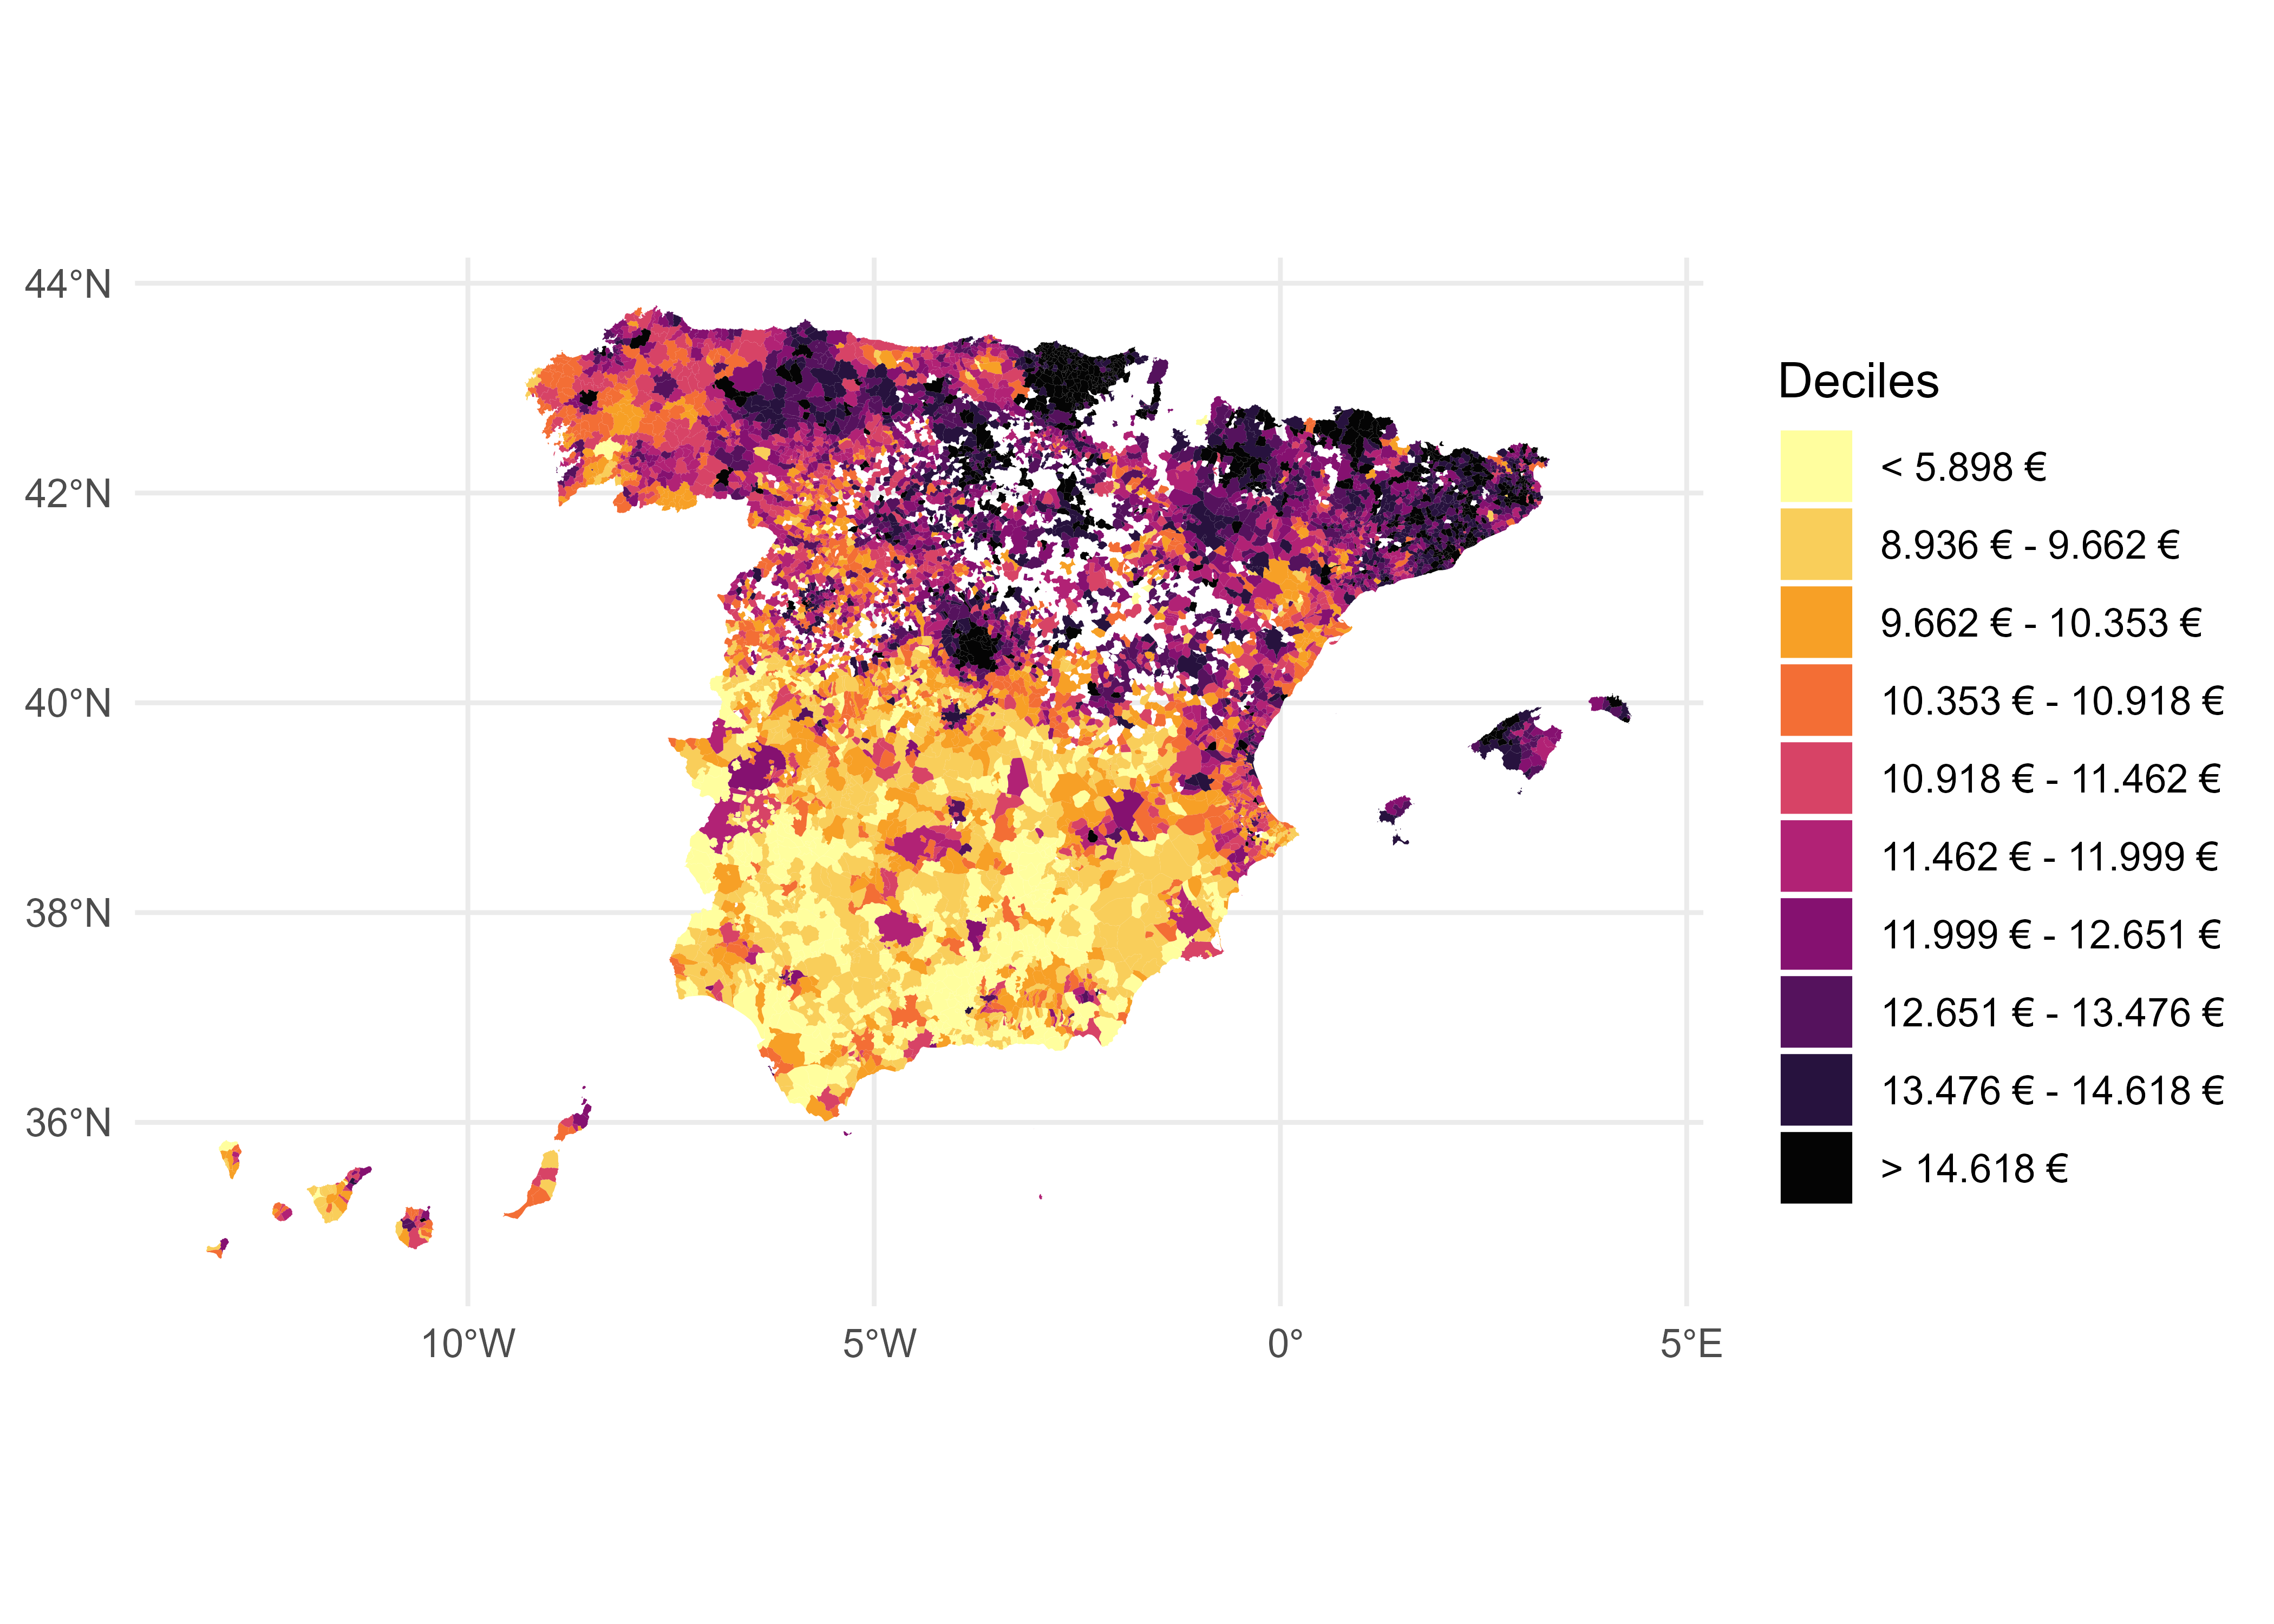
\includegraphics[width=0.6\linewidth]{_main_files/figure-latex/mapa-deciles-1} 

}

\caption{Mapa por deciles de renta media por persona (2019)}\label{fig:mapa-deciles}
\end{figure}

\begin{Shaded}
\begin{Highlighting}[]
\CommentTok{\# labs(}
\CommentTok{\#  title = "Renta neta media por persona",}
\CommentTok{\#  caption = "Datos: INE"}
\CommentTok{\# )}
\end{Highlighting}
\end{Shaded}

El mapa de la Fig. \ref{fig:mapa-deciles} ya permite observar patrones
geográficos, donde se ve una clara diferencia entre la Comunidades Autónomas del
Norte y las del Sur. Veamos una representación distina usando otras clases
diferentes

\begin{Shaded}
\begin{Highlighting}[]

\NormalTok{breaks\_e }\OtherTok{\textless{}{-}}\NormalTok{ equal}\SpecialCharTok{$}\NormalTok{brks}
\NormalTok{labels\_e }\OtherTok{\textless{}{-}} \FunctionTok{label\_fun}\NormalTok{(breaks\_e)}

\NormalTok{munis\_renta\_clean}\SpecialCharTok{$}\NormalTok{Equal }\OtherTok{\textless{}{-}} \FunctionTok{cut}\NormalTok{(munis\_renta\_clean}\SpecialCharTok{$}\StringTok{\textasciigrave{}}\AttributeTok{2019}\StringTok{\textasciigrave{}}\NormalTok{,}
  \AttributeTok{breaks =}\NormalTok{ breaks\_e,}
  \AttributeTok{labels =}\NormalTok{ labels\_e,}
  \AttributeTok{include.lowest =} \ConstantTok{TRUE}
\NormalTok{)}

\FunctionTok{ggplot}\NormalTok{(munis\_renta\_clean) }\SpecialCharTok{+}
  \CommentTok{\# Cambiamos la variable que usamos para crear el mapa}
  \FunctionTok{geom\_sf}\NormalTok{(}\FunctionTok{aes}\NormalTok{(}\AttributeTok{fill =}\NormalTok{ Equal), }\AttributeTok{color =} \ConstantTok{NA}\NormalTok{) }\SpecialCharTok{+}
  \FunctionTok{scale\_fill\_manual}\NormalTok{(}\AttributeTok{values =} \FunctionTok{hcl.colors}\NormalTok{(}\FunctionTok{length}\NormalTok{(labels\_e),}
    \StringTok{"Inferno"}\NormalTok{,}
    \AttributeTok{rev =} \ConstantTok{TRUE}
\NormalTok{  )) }\SpecialCharTok{+}
  \FunctionTok{theme\_minimal}\NormalTok{() }\CommentTok{\# +}
\end{Highlighting}
\end{Shaded}

\begin{figure}

{\centering 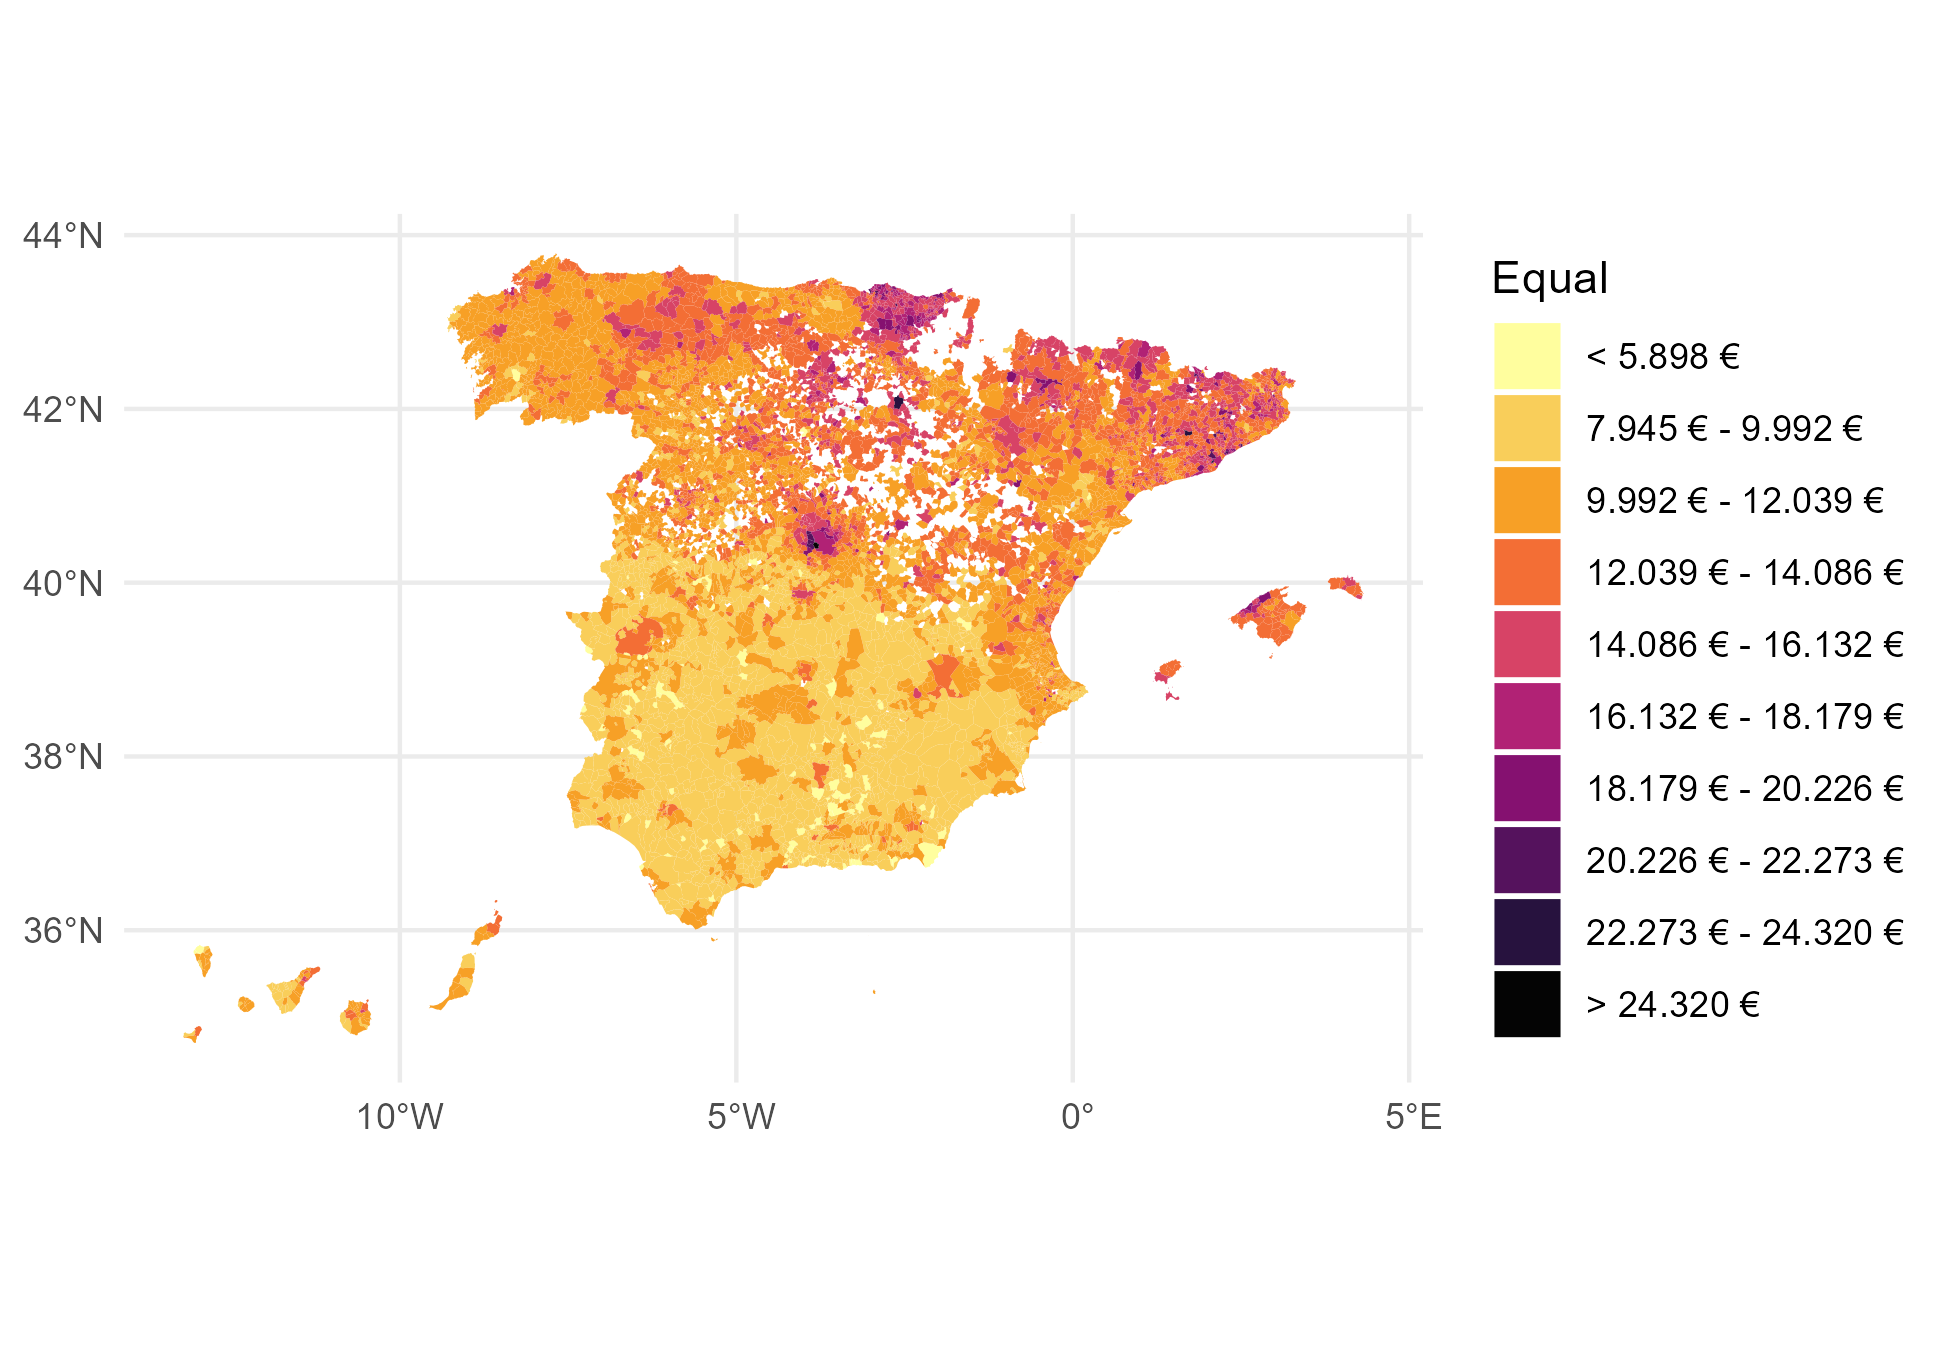
\includegraphics[width=0.6\linewidth]{_main_files/figure-latex/mapa-equal-1} 

}

\caption{Mapa por tramos de renta equidistantes de renta media por persona (2019)}\label{fig:mapa-equal}
\end{figure}

\begin{Shaded}
\begin{Highlighting}[]
\CommentTok{\# labs(}
\CommentTok{\#  title = "Renta neta media por persona",}
\CommentTok{\#  caption = "Datos: INE"}
\CommentTok{\# )}
\end{Highlighting}
\end{Shaded}

El mapa de la Fig. \ref{fig:mapa-deciles}, sin embargo, se parece más al mapa
de la Fig. \ref{fig:maparenta2} con los datos sin clasificar, donde el peso visual se concentra más
bien en los municipios con rentas mucho más altas que el resto (por encima de
18.000 €).

Véase a continuación el mismo mapa usando la clasificación Fisher-Jenks:

\begin{Shaded}
\begin{Highlighting}[]

\NormalTok{breaks\_f }\OtherTok{\textless{}{-}}\NormalTok{ fisher}\SpecialCharTok{$}\NormalTok{brks}
\NormalTok{labels\_f }\OtherTok{\textless{}{-}} \FunctionTok{label\_fun}\NormalTok{(breaks\_f)}

\NormalTok{munis\_renta\_clean}\SpecialCharTok{$}\StringTok{\textasciigrave{}}\AttributeTok{Fisher{-}Jenks}\StringTok{\textasciigrave{}} \OtherTok{\textless{}{-}} \FunctionTok{cut}\NormalTok{(munis\_renta\_clean}\SpecialCharTok{$}\StringTok{\textasciigrave{}}\AttributeTok{2019}\StringTok{\textasciigrave{}}\NormalTok{,}
  \AttributeTok{breaks =}\NormalTok{ breaks\_f,}
  \AttributeTok{labels =}\NormalTok{ labels\_f,}
  \AttributeTok{include.lowest =} \ConstantTok{TRUE}
\NormalTok{)}

\FunctionTok{ggplot}\NormalTok{(munis\_renta\_clean) }\SpecialCharTok{+}
  \CommentTok{\# Cambiamos la variable que usamos para crear el mapa}
  \FunctionTok{geom\_sf}\NormalTok{(}\FunctionTok{aes}\NormalTok{(}\AttributeTok{fill =} \StringTok{\textasciigrave{}}\AttributeTok{Fisher{-}Jenks}\StringTok{\textasciigrave{}}\NormalTok{), }\AttributeTok{color =} \ConstantTok{NA}\NormalTok{) }\SpecialCharTok{+}
  \FunctionTok{scale\_fill\_manual}\NormalTok{(}\AttributeTok{values =} \FunctionTok{hcl.colors}\NormalTok{(}\FunctionTok{length}\NormalTok{(labels\_f),}
    \StringTok{"Inferno"}\NormalTok{,}
    \AttributeTok{rev =} \ConstantTok{TRUE}
\NormalTok{  )) }\SpecialCharTok{+}
  \FunctionTok{theme\_minimal}\NormalTok{() }\SpecialCharTok{+}
  \FunctionTok{labs}\NormalTok{(}
    \AttributeTok{title =} \StringTok{"Renta neta media por persona"}\NormalTok{,}
    \AttributeTok{caption =} \StringTok{"Datos: INE"}
\NormalTok{  )}
\end{Highlighting}
\end{Shaded}

\begin{figure}

{\centering \includegraphics[width=0.6\linewidth]{_main_files/figure-latex/mapa-fisher-1} 

}

\caption{Mapa por tramos según Fisher-Jenks}\label{fig:mapa-fisher}
\end{figure}

En el mapa de la Fig. \ref{fig:mapa-deciles} se puede observar de una manera
más clara un cluster adicional de renta en la zona de Asturias y el norte de
León. Además, gracias a la escala de colores puede intuirse que este clúster de
renta no presenta valores tan altos como los observados en País Vasco o Madrid.

En conclusión, en el momento de realizar una visualización de datos es
importante conocer el dato a representar, así como entender algunas propiedades
básicas de la distribución subyacente. También se ha podido observar que hay
ciertas decisiones estéticas (datos continuos vs.~agrupados, escala de colores)
que tienen una influencia significativa en cómo se percibe la información
representada. Es responsabilidad del investigado encargado de
crear de la visualización el conocer
todos estos factores y aplicarlos de manera conveniente.

\hypertarget{caso-3.-distribuciuxf3n-espacial-de-los-delitos-cometidos-en-la-ciudad-de-valencia-en-el-auxf1o-2010.}{%
\section{Caso 3. Distribución espacial de los delitos cometidos en la ciudad de Valencia en el año 2010.}\label{caso-3.-distribuciuxf3n-espacial-de-los-delitos-cometidos-en-la-ciudad-de-valencia-en-el-auxf1o-2010.}}

Las técnicas de análisis de patrones de puntos analizan la distribución de
eventos geolocalizados que surgen al azar. La diferencia fundamental con otros
análisis que comprenden también el uso de localizaciones (como las temperaturas
mínimas medidas por estaciones meteorológicas) es que en este caso los puntos
representan eventos conocidos y aleatorios (por ejemplo, los delitos ocurridos
en una ciudad, accidentes de tráfico o incendios en una región). A diferencia de
otros eventos, como el ejemplo de las temperaturas mínimas, la ausencia de datos
no se debe a la ausencia de medición (es decir, no existe una estación meteorológica
en ese lugar), si no a que no se ha producido el evento en dicha localización.

\textbf{Objetivo de aprendizaje}:

El alumno debe ser capaz de conocer los datos de tipo patrones de punto,
identificarlos y representarlos adecuadamente.

\begin{itemize}
\tightlist
\item
  describir los ficheros. Hay que generar uno que sólo tenga 2010 y los datos
  que utilizamos. lo llamamos igual y vale todo
\end{itemize}

\begin{exercise}[Representación de la información sesgada]
\protect\hypertarget{exr:ex24}{}\label{exr:ex24}El presente análisis se va a realizar empleando RStudio, por lo que empezaremos
abriendo el programa y creando un nuevo script de R en \emph{Proyecto\textgreater File\textgreater New File\textgreater R
script}.
\end{exercise}

** habría que poner esto al inico de las 3 prácticas. comprobar.

\emph{Tarea 2: Importamos y describimos los datos objeto de estudio}

El primer paso consiste en importar la base de datos de crímenes en la ciudad de
Valencia. El archivo está en formato csv, por lo que usaremos el paquete \texttt{readr}
para importar los datos:

\begin{Shaded}
\begin{Highlighting}[]
\FunctionTok{library}\NormalTok{(readr)}
\FunctionTok{library}\NormalTok{(dplyr)}

\CommentTok{\# En este caso el archivo está en la carpeta "data" de nuestro proyecto}
\NormalTok{crimen }\OtherTok{\textless{}{-}} \FunctionTok{read\_csv}\NormalTok{(}\StringTok{"data/crime{-}data{-}Valencia.csv"}\NormalTok{)}


\FunctionTok{summary}\NormalTok{(crimen)}
\CommentTok{\#\textgreater{}    crime\_id          crime\_date         crime\_time        crime\_type       }
\CommentTok{\#\textgreater{}  Length:90247       Length:90247       Length:90247      Length:90247      }
\CommentTok{\#\textgreater{}  Class :character   Class :character   Class1:hms        Class :character  }
\CommentTok{\#\textgreater{}  Mode  :character   Mode  :character   Class2:difftime   Mode  :character  }
\CommentTok{\#\textgreater{}                                        Mode  :numeric                      }
\CommentTok{\#\textgreater{}                                                                            }
\CommentTok{\#\textgreater{}                                                                            }
\CommentTok{\#\textgreater{}      muni                year          month             week      }
\CommentTok{\#\textgreater{}  Length:90247       Min.   :2010   Min.   : 1.000   Min.   : 1.00  }
\CommentTok{\#\textgreater{}  Class :character   1st Qu.:2013   1st Qu.: 4.000   1st Qu.:14.00  }
\CommentTok{\#\textgreater{}  Mode  :character   Median :2016   Median : 7.000   Median :27.00  }
\CommentTok{\#\textgreater{}                     Mean   :2015   Mean   : 6.537   Mean   :26.65  }
\CommentTok{\#\textgreater{}                     3rd Qu.:2018   3rd Qu.: 9.000   3rd Qu.:38.00  }
\CommentTok{\#\textgreater{}                     Max.   :2020   Max.   :12.000   Max.   :53.00  }
\CommentTok{\#\textgreater{}       day           week\_day     week\_day\_name        crime\_hour   }
\CommentTok{\#\textgreater{}  Min.   :  1.0   Min.   :1.000   Length:90247       Min.   : 0.00  }
\CommentTok{\#\textgreater{}  1st Qu.: 96.0   1st Qu.:3.000   Class :character   1st Qu.: 5.00  }
\CommentTok{\#\textgreater{}  Median :187.0   Median :5.000   Mode  :character   Median :14.00  }
\CommentTok{\#\textgreater{}  Mean   :183.6   Mean   :4.323                      Mean   :12.52  }
\CommentTok{\#\textgreater{}  3rd Qu.:266.0   3rd Qu.:6.000                      3rd Qu.:19.00  }
\CommentTok{\#\textgreater{}  Max.   :366.0   Max.   :7.000                      Max.   :23.00  }
\CommentTok{\#\textgreater{}    crime\_lon         crime\_lat        atm\_dist          bank\_dist       }
\CommentTok{\#\textgreater{}  Min.   :{-}0.4296   Min.   :39.42   Min.   :   1.549   Min.   :   1.713  }
\CommentTok{\#\textgreater{}  1st Qu.:{-}0.3883   1st Qu.:39.46   1st Qu.: 380.535   1st Qu.: 133.908  }
\CommentTok{\#\textgreater{}  Median :{-}0.3749   Median :39.47   Median : 630.867   Median : 228.003  }
\CommentTok{\#\textgreater{}  Mean   :{-}0.3724   Mean   :39.47   Mean   : 790.228   Mean   : 305.315  }
\CommentTok{\#\textgreater{}  3rd Qu.:{-}0.3593   3rd Qu.:39.48   3rd Qu.: 986.897   3rd Qu.: 384.706  }
\CommentTok{\#\textgreater{}  Max.   :{-}0.3208   Max.   :39.53   Max.   :4838.847   Max.   :3411.537  }
\CommentTok{\#\textgreater{}     bar\_dist          cafe\_dist        industrial\_dist   market\_dist      }
\CommentTok{\#\textgreater{}  Min.   :   0.489   Min.   :   1.342   Min.   :   0.1   Min.   :   1.821  }
\CommentTok{\#\textgreater{}  1st Qu.: 149.879   1st Qu.: 133.274   1st Qu.: 268.4   1st Qu.: 487.874  }
\CommentTok{\#\textgreater{}  Median : 292.246   Median : 264.504   Median : 509.6   Median : 869.516  }
\CommentTok{\#\textgreater{}  Mean   : 392.072   Mean   : 360.275   Mean   : 675.2   Mean   :1008.414  }
\CommentTok{\#\textgreater{}  3rd Qu.: 507.701   3rd Qu.: 462.982   3rd Qu.: 909.9   3rd Qu.:1263.405  }
\CommentTok{\#\textgreater{}  Max.   :4352.380   Max.   :4237.915   Max.   :4703.9   Max.   :4855.407  }
\CommentTok{\#\textgreater{}  nightclub\_dist      police\_dist          pub\_dist        restaurant\_dist   }
\CommentTok{\#\textgreater{}  Min.   :   1.189   Min.   :   0.688   Min.   :   1.489   Min.   :   0.427  }
\CommentTok{\#\textgreater{}  1st Qu.: 468.164   1st Qu.: 455.810   1st Qu.: 190.150   1st Qu.:  73.401  }
\CommentTok{\#\textgreater{}  Median : 810.185   Median : 706.094   Median : 383.330   Median : 147.797  }
\CommentTok{\#\textgreater{}  Mean   : 930.501   Mean   : 875.246   Mean   : 496.472   Mean   : 223.875  }
\CommentTok{\#\textgreater{}  3rd Qu.:1256.269   3rd Qu.:1105.625   3rd Qu.: 665.599   3rd Qu.: 272.288  }
\CommentTok{\#\textgreater{}  Max.   :4700.567   Max.   :4765.745   Max.   :4168.869   Max.   :3746.536  }
\CommentTok{\#\textgreater{}    taxi\_dist           grid\_id         grid\_lon          grid\_lat    }
\CommentTok{\#\textgreater{}  Min.   :   2.441   Min.   :  8.0   Min.   :{-}0.4288   Min.   :39.42  }
\CommentTok{\#\textgreater{}  1st Qu.: 393.438   1st Qu.:173.0   1st Qu.:{-}0.3898   1st Qu.:39.46  }
\CommentTok{\#\textgreater{}  Median : 651.644   Median :215.0   Median :{-}0.3731   Median :39.47  }
\CommentTok{\#\textgreater{}  Mean   : 717.381   Mean   :210.8   Mean   :{-}0.3724   Mean   :39.47  }
\CommentTok{\#\textgreater{}  3rd Qu.: 931.083   3rd Qu.:248.0   3rd Qu.:{-}0.3620   3rd Qu.:39.48  }
\CommentTok{\#\textgreater{}  Max.   :4284.239   Max.   :398.0   Max.   :{-}0.3230   Max.   :39.53}
\end{Highlighting}
\end{Shaded}

\textbf{¿Qué información contiene los datos que se van a analizar?} Este archivo contiene en total
90.247 registros, y
proporciona 28 campos asociados a cada registro.

Entre los campos disponibles, destacamos los campos \texttt{crime\_lon} y \texttt{crime\_lat}:
Son las coordenadas en las que se produjo el crimen.

\begin{exercise}[CRS de las coordenadas]
\protect\hypertarget{exr:ex26}{}\label{exr:ex26}Determine el CRS en el que se encuentras las coordenadas del conjuto de datos
\texttt{crimen}, etiquetas con \texttt{crime\_lon} y \texttt{crime\_lat}
\end{exercise}

\begin{table}

\caption{\label{tab:coods-lonlat}Crímenes en Valencia; Coordenadas}
\centering
\begin{tabular}[t]{r|r}
\hline
crime\_lon & crime\_lat\\
\hline
-0.3826325 & 39.46332\\
\hline
-0.3906850 & 39.43517\\
\hline
-0.3747971 & 39.47927\\
\hline
-0.3992082 & 39.47982\\
\hline
-0.3596011 & 39.46740\\
\hline
-0.3552423 & 39.47461\\
\hline
\end{tabular}
\end{table}

Obsérvese que, las coordenadas parecen corresponder con longitudes y latitudes,
ya que como se explicó el rango posible de valores es \([-180, 180]\) (para
longitudes) y \([-90, 90]\) (para latitudes):

\begin{exercise}[Proyección y representación de localizaciones]
\protect\hypertarget{exr:ex27}{}\label{exr:ex27}Convierta el objeto \texttt{crimen} a un objecto \texttt{sf} llamado \texttt{crimen\_sf}, teniendo en
cuenta el sistema CRS más adecuado.
A modo de recordatorio, el CRS correspondiente a coordenadas
geográficas longitud/latitud es \textbf{EPSG:4326}.

Una vez proyectdas las coordenadas represéntelas en un mapa. Si lo desea
puede usar una imagen de fondo con la función \texttt{esp\_getTiles} de la librería
\texttt{mapSpain}.
\end{exercise}

\begin{Shaded}
\begin{Highlighting}[]

\FunctionTok{library}\NormalTok{(sf)}
\CommentTok{\# Objeto sf sin CRS}

\NormalTok{crimen\_sf }\OtherTok{\textless{}{-}} \FunctionTok{st\_as\_sf}\NormalTok{(}
\NormalTok{  crimen,}
  \AttributeTok{coords =} \FunctionTok{c}\NormalTok{(}
    \StringTok{"crime\_lon"}\NormalTok{,}
    \StringTok{"crime\_lat"}
\NormalTok{  ),}
  \AttributeTok{crs =} \FunctionTok{st\_crs}\NormalTok{(}\DecValTok{4326}\NormalTok{)}
\NormalTok{)}

\CommentTok{\# Comprobamos con un mapa base}

\FunctionTok{library}\NormalTok{(mapSpain)}
\FunctionTok{library}\NormalTok{(ggplot2)}

\CommentTok{\# Usamos imagen como mapa de fondo}
\NormalTok{tile }\OtherTok{\textless{}{-}} \FunctionTok{esp\_getTiles}\NormalTok{(crimen\_sf, }\StringTok{"IDErioja"}\NormalTok{,}
  \AttributeTok{zoommin =} \DecValTok{1}\NormalTok{,}
  \AttributeTok{crop =} \ConstantTok{TRUE}
\NormalTok{)}

\FunctionTok{ggplot}\NormalTok{() }\SpecialCharTok{+}
  \FunctionTok{layer\_spatraster}\NormalTok{(tile) }\SpecialCharTok{+}
  \FunctionTok{geom\_sf}\NormalTok{(}
    \AttributeTok{data =}\NormalTok{ crimen\_sf,}
    \AttributeTok{col =} \StringTok{"blue"}\NormalTok{,}
    \AttributeTok{size =} \FloatTok{0.3}\NormalTok{,}
    \AttributeTok{alpha =} \FloatTok{0.3}
\NormalTok{  )}
\end{Highlighting}
\end{Shaded}

\begin{figure}

{\centering \includegraphics[width=0.6\linewidth]{_main_files/figure-latex/crimen1-1} 

}

\caption{Crímenes en Valencia}\label{fig:crimen1}
\end{figure}

¿Hay algún patrón en la ocurrencia de crímenes?**

En la Fig. \ref{fig:crimen1} podemos intuir ciertos patrones en la ocurrencia
de crímenes. Por ejemplo, parecen concentrarse en zonas céntricas y no hay
crímenes registrados en la zona del puerto.

Para el siguiente análisis, vamos a analizar el patrón de crímenes del año 2010.

** diego, engancha esto con lo anterior, porque sólo vamos a usar un año, y así
evitamos problemas

\begin{Shaded}
\begin{Highlighting}[]
\NormalTok{crimen\_2010\_sf }\OtherTok{\textless{}{-}}\NormalTok{ crimen\_sf }\SpecialCharTok{\%\textgreater{}\%}
  \FunctionTok{filter}\NormalTok{(}
\NormalTok{    year }\SpecialCharTok{==} \StringTok{"2010"}
\NormalTok{  )}

\FunctionTok{ggplot}\NormalTok{() }\SpecialCharTok{+}
  \FunctionTok{layer\_spatraster}\NormalTok{(tile) }\SpecialCharTok{+}
  \FunctionTok{geom\_sf}\NormalTok{(}
    \AttributeTok{data =}\NormalTok{ crimen\_2010\_sf,}
    \AttributeTok{col =} \StringTok{"blue"}\NormalTok{,}
    \AttributeTok{size =} \FloatTok{0.3}\NormalTok{,}
    \AttributeTok{alpha =} \FloatTok{0.3}
\NormalTok{  )}
\end{Highlighting}
\end{Shaded}

\begin{figure}

{\centering \includegraphics[width=0.6\linewidth]{_main_files/figure-latex/crimen2-1} 

}

\caption{Crímenes en Valencia (2010)}\label{fig:crimen2}
\end{figure}

\begin{itemize}
\tightlist
\item
\end{itemize}

El paquete \texttt{spatstat} (\citet{spatstat_2005}) es el paquete de referencia cuando se
trabaja con patrones de puntos

Siguiendo el anterior ejemplo, vamos a analizar el patrón de crímenes en el año
2010. Además, en el análisis de patrones de puntos es necesario delimitar la
ventana espacial de observación (owin). En este caso será el municipio de
Valencia.

\begin{exercise}[Análisis de patrones con `spatstat`]
\protect\hypertarget{exr:ex37}{}\label{exr:ex37}FALTA
\end{exercise}

\begin{Shaded}
\begin{Highlighting}[]

\CommentTok{\# Extraigo Valencia con mapSpain}

\NormalTok{valencia }\OtherTok{\textless{}{-}} \FunctionTok{esp\_get\_munic}\NormalTok{(}\AttributeTok{munic =} \StringTok{"\^{}Valencia$"}\NormalTok{) }\SpecialCharTok{\%\textgreater{}\%}
  \CommentTok{\# Necesito proyectar, en este caso usamos ETRS89{-}UTM huso 30 EPSG:25830}
  \FunctionTok{st\_transform}\NormalTok{(}\DecValTok{25830}\NormalTok{)}



\FunctionTok{library}\NormalTok{(spatstat)}
\CommentTok{\# Necesitamos un recinto de observación: owin}

\NormalTok{val\_owin }\OtherTok{\textless{}{-}} \FunctionTok{as.owin}\NormalTok{(valencia)}

\CommentTok{\# Extraemos las coordenadas de los crímenes. Han de estar en el mismo CRS}
\CommentTok{\# que el owin}

\NormalTok{coords }\OtherTok{\textless{}{-}}\NormalTok{ crimen\_2010\_sf }\SpecialCharTok{\%\textgreater{}\%}
  \FunctionTok{st\_transform}\NormalTok{(}\DecValTok{25830}\NormalTok{) }\SpecialCharTok{\%\textgreater{}\%}
  \FunctionTok{st\_coordinates}\NormalTok{()}

\NormalTok{mydata\_ppp }\OtherTok{\textless{}{-}} \FunctionTok{ppp}\NormalTok{(}
  \AttributeTok{x =} \FunctionTok{as.numeric}\NormalTok{(coords[, }\DecValTok{1}\NormalTok{]),}
  \AttributeTok{y =} \FunctionTok{as.numeric}\NormalTok{(coords[, }\DecValTok{2}\NormalTok{]),}
  \AttributeTok{window =}\NormalTok{ val\_owin}
\NormalTok{)}

\FunctionTok{plot}\NormalTok{(mydata\_ppp)}
\end{Highlighting}
\end{Shaded}

\begin{center}\includegraphics[width=0.6\linewidth]{_main_files/figure-latex/objeto_ppp-1} \end{center}

ERROR EN EL NOMBRE mydata\_ppp, es por el guión.

\begin{exercise}[Información del objeto `mydatappp`]
\protect\hypertarget{exr:ex38}{}\label{exr:ex38}FALTA
\end{exercise}

¿Qué información contiene nuestro objeto en formato ppp?

\begin{Shaded}
\begin{Highlighting}[]
\FunctionTok{summary}\NormalTok{(mydata\_ppp)}
\CommentTok{\#\textgreater{} Planar point pattern:  5332 points}
\CommentTok{\#\textgreater{} Average intensity 3.917619e{-}05 points per square unit}
\CommentTok{\#\textgreater{} }
\CommentTok{\#\textgreater{} *Pattern contains duplicated points*}
\CommentTok{\#\textgreater{} }
\CommentTok{\#\textgreater{} Coordinates are given to 1 decimal place}
\CommentTok{\#\textgreater{} i.e. rounded to the nearest multiple of 0.1 units}
\CommentTok{\#\textgreater{} }
\CommentTok{\#\textgreater{} Window: polygonal boundary}
\CommentTok{\#\textgreater{} 4 separate polygons (no holes)}
\CommentTok{\#\textgreater{}            vertices      area relative.area}
\CommentTok{\#\textgreater{} polygon 1         4   1977930       0.01450}
\CommentTok{\#\textgreater{} polygon 2        82 131953000       0.97000}
\CommentTok{\#\textgreater{} polygon 3         7    958085       0.00704}
\CommentTok{\#\textgreater{} polygon 4         7   1214060       0.00892}
\CommentTok{\#\textgreater{} enclosing rectangle: [720573.4, 735116.6] x [4351274, 4382995] units}
\CommentTok{\#\textgreater{}                      (14540 x 31720 units)}
\CommentTok{\#\textgreater{} Window area = 136103000 square units}
\CommentTok{\#\textgreater{} Fraction of frame area: 0.295}
\CommentTok{\#\textgreater{} }
\CommentTok{\#\textgreater{} *** 6 illegal points stored in attr(,"rejects") ***}
\end{Highlighting}
\end{Shaded}

\emph{Tarea 4: .}

Es importante determinar si los puntos se distribuyen al azar o tienen algún
patrón. Por ello, lo primero que haremos será representar el objeto \texttt{feb\_ppp} y
superponer unos cuadrantes para su comportamiento (véase Fig.
\ref{fig:cuadrante}).

\begin{exercise}[Cálculo de la densidad de los delitos en Valencia en 2010 mediante cuadrantes]
\protect\hypertarget{exr:ex37}{}\label{exr:ex37}FALTA
\end{exercise}

** ESte mapa se puede poner un poco más mono?? Yo ya lo he arregado un poco

\begin{Shaded}
\begin{Highlighting}[]
\DocumentationTok{\#\# Hallamos los cuadrantes}
\NormalTok{cuadrante }\OtherTok{\textless{}{-}} \FunctionTok{quadratcount}\NormalTok{(mydata\_ppp,}
  \AttributeTok{nx =} \DecValTok{5}\NormalTok{,}
  \AttributeTok{ny =} \DecValTok{5}
\NormalTok{)}

\DocumentationTok{\#\# Dibujamos el número de crímenes que hay en cada cuadrante}
\FunctionTok{plot}\NormalTok{(mydata\_ppp, }\AttributeTok{pch =} \StringTok{"+"}\NormalTok{, }\AttributeTok{main =} \StringTok{""}\NormalTok{, }\AttributeTok{cex =} \FloatTok{0.3}\NormalTok{)}
\FunctionTok{plot}\NormalTok{(cuadrante, }\AttributeTok{add =} \ConstantTok{TRUE}\NormalTok{, }\AttributeTok{col =} \StringTok{"red"}\NormalTok{, }\AttributeTok{cex =} \FloatTok{0.6}\NormalTok{, }\AttributeTok{lwd =} \DecValTok{2}\NormalTok{)}
\end{Highlighting}
\end{Shaded}

\begin{figure}

{\centering \includegraphics[width=0.6\linewidth]{_main_files/figure-latex/cuadrante-1} 

}

\caption{Crímenes en Valencia por cuadrantes (2010)}\label{fig:cuadrante}
\end{figure}

Como se puede apreciar en la Fig. \ref{fig:cuadrante} hay cuadrantes que
registran cero crímenes y otros que registran hasta 2.860 crímenes.

\begin{exercise}[Estimación de la densidad de los delitos en Valencia en 2010 mediante de patrones de puntos]
\protect\hypertarget{exr:ex37}{}\label{exr:ex37}FALTA

density \{stats\}
\end{exercise}

\begin{Shaded}
\begin{Highlighting}[]

\CommentTok{\# Permite ver la variación local de la intensidad, graficando la estimación kernel de la intensidad.}
\NormalTok{densidad }\OtherTok{\textless{}{-}} \FunctionTok{density}\NormalTok{(mydata\_ppp)}

\FunctionTok{plot}\NormalTok{(densidad, }\AttributeTok{main =} \StringTok{" "}\NormalTok{)}
\FunctionTok{points}\NormalTok{(mydata\_ppp, }\AttributeTok{pch =} \StringTok{"+"}\NormalTok{, }\AttributeTok{cex =} \FloatTok{0.5}\NormalTok{)}
\end{Highlighting}
\end{Shaded}

\begin{figure}

{\centering \includegraphics[width=0.6\linewidth]{_main_files/figure-latex/intensidad-ppp-1} 

}

\caption{Estimación kernel de la intensidad de crímenes en la ciudad de Valencia }\label{fig:intensidad-ppp}
\end{figure}

En la Fig. \ref{fig:intensidad-ppp} se muestra la estimación kernel
de la densidad de patrones de puntos Los conocimientos teóricos necesarios para llevar a cabo
este tipo de estimación superan el ámbito de este manual. El objetivo
de este ejemplo es meramente ilustrativo.

\hypertarget{appendix-anexo}{%
\appendix}


\hypertarget{crsproy}{%
\chapter{Tipos de CRS proyectados}\label{crsproy}}

Existen varias familias de proyecciones, que se pueden clasificar de diversas
maneras: por tipo de superficie de proyección y por métrica a preservar.

\hypertarget{por-tipo-de-superficie-de-proyecciuxf3n}{%
\section{Por tipo de superficie de proyección}\label{por-tipo-de-superficie-de-proyecciuxf3n}}

El proceso de trasladar puntos de una esfera a un plano puede plantearse de
manera práctica como el ejercicio de envolver una esfera con una superificie
plana (como una hoja de papel) y trasladar los puntos de la esfera de manera
lineal al punto de la superficie plana más cercano a ella. La Fig.
\ref{fig:fi-proys} muestra estos tres tipos de proyección.

\begin{figure}

{\centering \includegraphics[width=0.6\linewidth]{img/tipos_proy} 

}

\caption{Tipos de proyección por superficie de proyección}\label{fig:fi-proys}
\end{figure}

A partir de este ejercicio, se plantean tres posibles soluciones (cilíndrica,
cónica y acimutal o planar), dependiendo del tipo de superficie que se use para
proyectar.

\begin{itemize}
\tightlist
\item
  \textbf{Proyecciones cilíndricas}: Son aquellas proyecciones donde la superficie
  de proyección conforma un cilindro alrededor de la Tierra. Una de las
  proyecciones cilíndricas más conocidas es la \textbf{proyección de Mercator} (Ver
  Fig. \ref{fig:mercator}).
\end{itemize}

\begin{figure}

{\centering \includegraphics[width=0.4\linewidth]{img/mercator} 

}

\caption{Proyección Mercator}\label{fig:mercator}
\end{figure}

\begin{itemize}
\tightlist
\item
  \textbf{Proyecciones cónicas}: En este tipo de proyecciones, se plantea la
  superficie de proyección como una forma cónica. Como ejemplo, la
  \textbf{proyección cónica equiáreas de Albers} es una de las proyecciones que más
  suele usarse en la representación de mapas de América del Norte (Ver Fig.
  \ref{fig:albers}).
\end{itemize}

\begin{figure}

{\centering \includegraphics[width=0.4\linewidth]{img/albers_conic} 

}

\caption{Proyección cónica equiáreas de Albers}\label{fig:albers}
\end{figure}

\begin{itemize}
\tightlist
\item
  \textbf{Proyecciones acimutales o planares:} En este tipo de proyección se
  proyecta una porción de la Tierra sobre un plano que es tangente a la misma
  en el punto de referencia. Como ejemplos de proyecciones acimutales podemos
  destacar la \textbf{proyección ortográfica} (Ver Fig. \ref{fig:orto}).
\end{itemize}

\begin{figure}

{\centering \includegraphics[width=0.4\linewidth]{img/orto} 

}

\caption{Proyección ortogonal}\label{fig:orto}
\end{figure}

\hypertarget{por-muxe9trica-a-preservar}{%
\section{Por métrica a preservar}\label{por-muxe9trica-a-preservar}}

Es importante tener en cuenta que cualquier proyección de la superficie de la
Tierra produce distorsiones en una o varias características geográficas. Como
ejemplo clásico, la proyección de Mercator produce distorsiones del \textbf{tamaño}
especialmente en aquellas regiones más cercanas a los polos (Groenlandia, que la
proyección de Mercator presenta una área similar a la de África, tiene menor
superficie real que Argelia). Otras de las métricas que suele verse
distorsionada son la \textbf{distancia} entre dos puntos geográficos, la
\textbf{dirección} o la \textbf{forma} de regiones de la Tierra.

A lo largo de la Historia se han desarrollado diversas proyecciones cuyo
objetivo es preservar alguna o varias de las propiedades mencionadas
anteriormente, sin embargo es importante destacar que \textbf{no existe una proyección
que sea capaz de preservar todas las métricas a la vez}.

Según la metrica a presevar, las proyecciones se pueden clasificar en:

\begin{itemize}
\tightlist
\item
  \textbf{Proyecciones conformales:} Intentan preservar los \textbf{ángulos} que se
  forman en la superficie terrestre. Por ejemplo, la proyección de Mercator
  representa ángulos rectos en las intersecciones de los paralelos y los
  meridianos (Ver Fig. \ref{fig:conform}).
\end{itemize}

\begin{figure}

{\centering \includegraphics[width=0.3\linewidth]{img/conform} 

}

\caption{Ejemplo de proyección conformal: Mercator}\label{fig:conform}
\end{figure}

\begin{itemize}
\tightlist
\item
  \textbf{Proyecciones equivalentes}: Preservan las proporciones de las \textbf{áreas},
  provocando a su vez deformaciones en el resto de características, como la
  forma o los ángulos. La proyección acimutal equivalente de Lambers es un
  tipo de proyección equivalente (Ver Fig. \ref{fig:equiv}).
\end{itemize}

\begin{figure}

{\centering \includegraphics[width=0.3\linewidth]{img/equiv} 

}

\caption{Ejemplo de proyección equivalente: Proyección acimutal equivalente de Lambers}\label{fig:equiv}
\end{figure}

\begin{itemize}
\tightlist
\item
  \textbf{Proyecciones equidistantes:} Preservan la \textbf{distancia} entre dos puntos
  geográficos específicos. Por ejemplo, la proyección Plate carré preserva la
  distancia entre el Polo Norte y el Polo Sur (Ver Fig. \ref{fig:equidist}).
\end{itemize}

\begin{figure}

{\centering \includegraphics[width=0.3\linewidth]{img/equidist} 

}

\caption{Ejemplo de proyección equidistante: Platé carre}\label{fig:equidist}
\end{figure}

\begin{itemize}
\tightlist
\item
  \textbf{Proyecciones de compromiso}: No intentan preservar ninguna métrica en
  concreto. En su lugar, se centran en intentar encontrar un \textbf{equilibrio}
  entre las diversas distorsiones que provocan para intentar dar una
  representación más o menos representativa de la superficie terrestre. La
  proyección de Winkel Tripel, usada en los mapas de National Geographic, es
  un ejemplo de proyección de compromiso (Ver Fig. \ref{fig:comp}).
\end{itemize}

\begin{figure}

{\centering \includegraphics[width=0.3\linewidth]{img/comp} 

}

\caption{Ejemplo de proyección de compromiso: Winkel Tripel}\label{fig:comp}
\end{figure}

En los anteriores ejemplos se ha añadido a cada proyección la \textbf{indicatriz de
Tissot}. Ésta consiste en una serie de círculos imaginarios de igual área
distribuidos sobre la superficie esférica de la Tierra en determinados puntos.
De este manera, al presentar la indicatriz de Tissot en una proyección
específica, se puede entender de una manera intuitiva la distorsión provocada
por dicha proyección, ya que los círculos se ven distorsionados o preservados
según los parámetros y la naturaleza de la proyección en cuestión.

\hypertarget{referencias}{%
\chapter{Referencias}\label{referencias}}

LO PONEMOS EN OTRO .RMD??

  \bibliography{book.bib}

\end{document}
